%USE XeLaTeX compiler!!

\documentclass[12pt,letterpaper]{article}
\usepackage[lmargin=1.2in,rmargin=1.2in,tmargin=1in,bmargin=1in]{geometry}
\usepackage[bf,tiny]{titlesec}
%\usepackage{fontspec,xltxtra,xunicode}
    	%\defaultfontfeatures{Mapping=tex-text}
%\usepackage[utf8]{inputenc}
%\usepackage[utf8]{fontenc}
%\setmainfont{Junicode}

\usepackage{setspace}
%\usepackage{gb4e}
\let\eachwordone=\it %italicise the first line of examples
\usepackage[sort]{natbib}
\bibpunct[: ]{(}{)}{,}{a}{}{,}
\usepackage{afterpage}
\usepackage{graphicx}

%%% your packages here; please use sparingly and for things you actually need (not for aesthetics)

% extra packages
\usepackage{placeins} %to enable float barriers
\usepackage{CJKutf8} %chinese caracthers
\usepackage[table,dvipsnames]{xcolor} %for specifying colors
\usepackage{amsmath} % for equations
\usepackage{booktabs} % for nice looking tables
\usepackage{longtable} %for tables stretching several pages
\usepackage{pdflscape} %for making things landscape
\usepackage{multirow} %merging rows in tables
\usepackage{rotating} %for sideways figures
\usepackage{caption} %for making subfigures
\usepackage{subcaption} %for making subfigures
\usepackage{newfloat} %making it possible to treat lists as floats
\DeclareFloatingEnvironment[placement={!ht},name=List]{mylist} %setting a float environment for lists
\usepackage{enumitem} %make it possible to have other enumerate items, like roman numerals
\usepackage{hyperref} %for nice looking links
\hypersetup{
    colorlinks=true, %set true if you want colored links
    linktoc=all,     %set to all if you want both sections and subsections linked
    linkcolor=violet,  %choose some color if you want links to stand out
            urlcolor=blue,
            citecolor=Thistle,
}

%define special colors for fonts and tables
\definecolor{spec_color_blue}{HTML}{7D81F5}
\definecolor{spec_color_lightgreen}{HTML}{81F093}
\definecolor{spec_color_darkgreen}{HTML}{0B8C1F}
\definecolor{spec_color_orange}{HTML}{FFB87A}
\definecolor{spec_color_red}{HTML}{FFD9E0}
\definecolor{spec_color_yellow}{HTML}{FCFFA8}




%%% preamble
\title{Disentangling Ancestral State Reconstruction in Historical Linguistics - comparing classic approaches and new methods with Oceanic grammar}
\author{Hedvig Skirgård}



\begin{document}
%\def\code#1{\texttt{#1}}

\thispagestyle{empty}


\maketitle
\thispagestyle{empty}


%\textcolor{red}{This is a first draft based on the chapter text. I've modified it, and I'm in the process of modifying further. }



\begin{abstract}

Ancestral State Reconstruction (ASR) is an essential part of historical linguistics (HL). Conventional ASR in HL relies on three core principles: fewest changes on the tree,  plausibility of changes and plausibility of the resulting combinations of features in proto-languages. This approach has some problems, in particular the definition of what is plausible and the disregard of branch lengths. This study compares the classic approach of ASR to computational tools (Maximum Parsimony and Maximum Likelihood), conceptually and practically. Computational models have the advantage of being more transparent, consistent and replicable, and the disadvantage of lacking nuanced knowledge and context. Using data from the structural database Grambank, I compare reconstructions of the grammar of ancestral Oceanic languages from the historical linguistics literature to those achieved by computational means. The results show that there is a high degree of agreement between manual and computational approaches, with a tendency for classical HL to agree more with the approaches that ignore branch lengths. Taking into account branch lengths explicitly is more conceptually sound, as such the field of historical linguistics should engage in improving methods in this direction. A combination of computational methods and qualitative knowledge is possible in future and would be of great benefit.

%Reconstruction is an essential part of historical linguistics. Conventional reconstruction in historical linguistics (HL) infers states in proto-languages by three core principles: assume the fewest changes on the tree, assume plausible changes, and assume plausible combinations of features in proto-languages. However, there is no clear consensus on how to weigh the principles against each other, and many studies are not fully transparent regarding how precisely the principles are applied. This allows for subjective differences between studies which are hard to discern and replicate. This study aims to better understand the toolbox of historical linguistics in general and Oceanic grammatical history in particular by comparing the reconstruction of structural features by classical historical linguists to computational reconstructions with explicit and transparent mechanisms: Maximum Parsimony (MP) and Marginal Maximum Likelihood (ML). MP is similar to conventional HL in that it infers the fewest amounts of changes along the tree. ML on the other hand infers rates of change based on the distribution of values and takes into account branch lengths. In addition, we explore an even simpler method of reconstruction, which ignores tree structure and takes into account only the most common feature in the daughter languages. The results indicate that all methods applied achieve a high level of concordance with predictions from historical linguistics, which lets us understand the mechanisms of CM better. The more methodology is made explicit, the better off we are as a field.

% ste says: https://www.facebook.com/alan.elliott.125/posts/pfbid022H8vUKQxqKEE1e64DTcaJqXLDdruJEP8kpj5M89UtV6z8HHSTTTtYJVMVhZuBhsHl

%There are two possible
%This could indicate that historical linguists mainly make statements about the grammar of Oceanic proto-languages where they have a high amount of certainty, 

%The results show that CM produces reconstructions that are most similar to those generated by MP or MC. This suggests that, at least for this sample of languages and features, CM does not appear to take branch lengths into account. The methodological drawbacks of using MP and MC imply that we should possibly re-evaluate the way reconstruction is done in historical linguistics and take into account insights from new approaches, such as ML which makes sound assumptions which are likely to give better estimations of the state of proto-languages.


%Historical linguists use the comparative method to find sound correspondences, to reconstruct unattested forms and structures of proto-languages and to propose subgroups. Part of this process can be done computationally with new methods such as Maximum Likelihood. Such methods are more explicit in terms of the assumed underlying tree structure, data weighting etc. Studies in historical linguistics are not always as explicit. In this paper, we attempt to reconstruct the assumptions and implicit inner workings of the comparative method by comparing reconstructions made "by hand" by historical linguists to those derived from computational means. We also address areas of conflicts where different historical linguistics scholars disagree and evaluate what we can learn from computational methods regarding these issues. We estimate the grammatical structures of Oceanic languages in particular, using the Grambank dataset and trees published by Glottolog and \citet{grayetal_2009}. The results show that classical historical linguistics, for this dataset and trees, appears to mainly be an application of Maximum Parsimony, and we further discuss what this implies for the field of reconstruction of proto-languages. In the cases where historical linguists disagree, the results further show that the most likely scenario is that proto-polynesian was ergative.
\end{abstract}


\noindent\textbf{Keywords:} oceanic languages, ancestral state reconstruction, grammar


%\tableofcontents

%\newpage


\section{Introduction}
\label{acr:intro}
Historical linguistics offers us a unique and insightful window into our human past. By reconstructing the paths languages take, we can learn about our history and infer the migration paths of people and cultures. By reconstructing the words, sounds and grammar of ancient languages, we can learn about communities long gone. Historical linguistics is devoted to this endeavour and has made great strides in our understanding of human history since its inception. The field has established methods that have enabled us to classify languages into language families and reconstruct words and sounds of proto-languages (unobserved ancestors of observed languages). Conclusions from historical linguistics are also influential in other historical sciences, for example archaeology (c.f. \citet[S364]{bellwood2011holocene}).

Scholars who work in historical linguistics produce valuable and greatly inspiring work and they possess a wealth of knowledge not only of the languages themselves, but also the cultures, societies and history of the region. At times, it is difficult to be explicit about all the background information and context that goes into an analysis in historical linguistics --- which makes it hard for someone else to replicate and examine the study thoroughly. When the information is made explicit in publications, it can be hard to aggregate across publications while keeping definitions and weights consistent.

In this study, we focus on one particular subset of the historical linguistics toolbox --- the inference of earlier states of languages --- and outline how computational approaches can be a complement that serves to increase speed, transparency and consistency. We discuss the underlying mechanisms of the conventional ``manual'' approaches to reconstruction in historical linguistics and compare the conceptual framework to computational alternatives. As a practical example, we compare reconstructions of Oceanic grammar. This study makes visible opportunities for methodological expansion that can be made by incorporating computational approaches into mainstream historical linguistics.

Historical linguists typically engage in three different tasks simultaneously: a) the identification of cognates and sound correspondences in languages, b) the inference of sub-grouping (networks/trees)\footnote{C.f. how biological cladistics finds relationships between species based on shared derived characteristics from common ancestors \citep[16-17]{maclaurin2008biodiversity})} and c) the inference of sounds/forms/patterns in proto-languages (Ancestral State Reconstruction = ASR). In conventional approaches in historical linguistics, these three tasks are done at the same time and inform each other --- they are necessarily interlinked. However, in historical analysis of biology and cultural evolution, these tasks are more separated out. Fig. \ref{fig:HL_tasks} illustrates these three tasks for four different kinds of material: words (sounds \& cognates), grammar, genes and biological features. The arrows indicate task workflow with information on words leading to the construction of trees, which in turn enables ASR on lexicon and grammar. This is mirrored in the biological sciences, with genome serving as the bases for the trees which then make ASR possible. The feedback loop between tree construction and ASR in the classical analysis of cognates and sound correspondences is illustrated with circular arrows forming a loop. The same is true of biological traits where biologist care about not predicting impossible ancestral states \citep{schulmeister2004comparative} and may therefore revise the tree-building if these occur. Furthermore, both linguists and biologist may return and re-examine their original classification of their data (task a; cognate coding, sample labelling, sequence alignment etc.) given the outcome of ASR (c.f. re-estimating sequence alignment in genetics while estimating trees \citep{10.1093/bioinformatics/btab129}. The three tasks are not necessarily independent in the biological sciences, but it is possible to carry them out separately and the links between them are explicit. 

\begin{sidewaysfigure}[p]
\centering
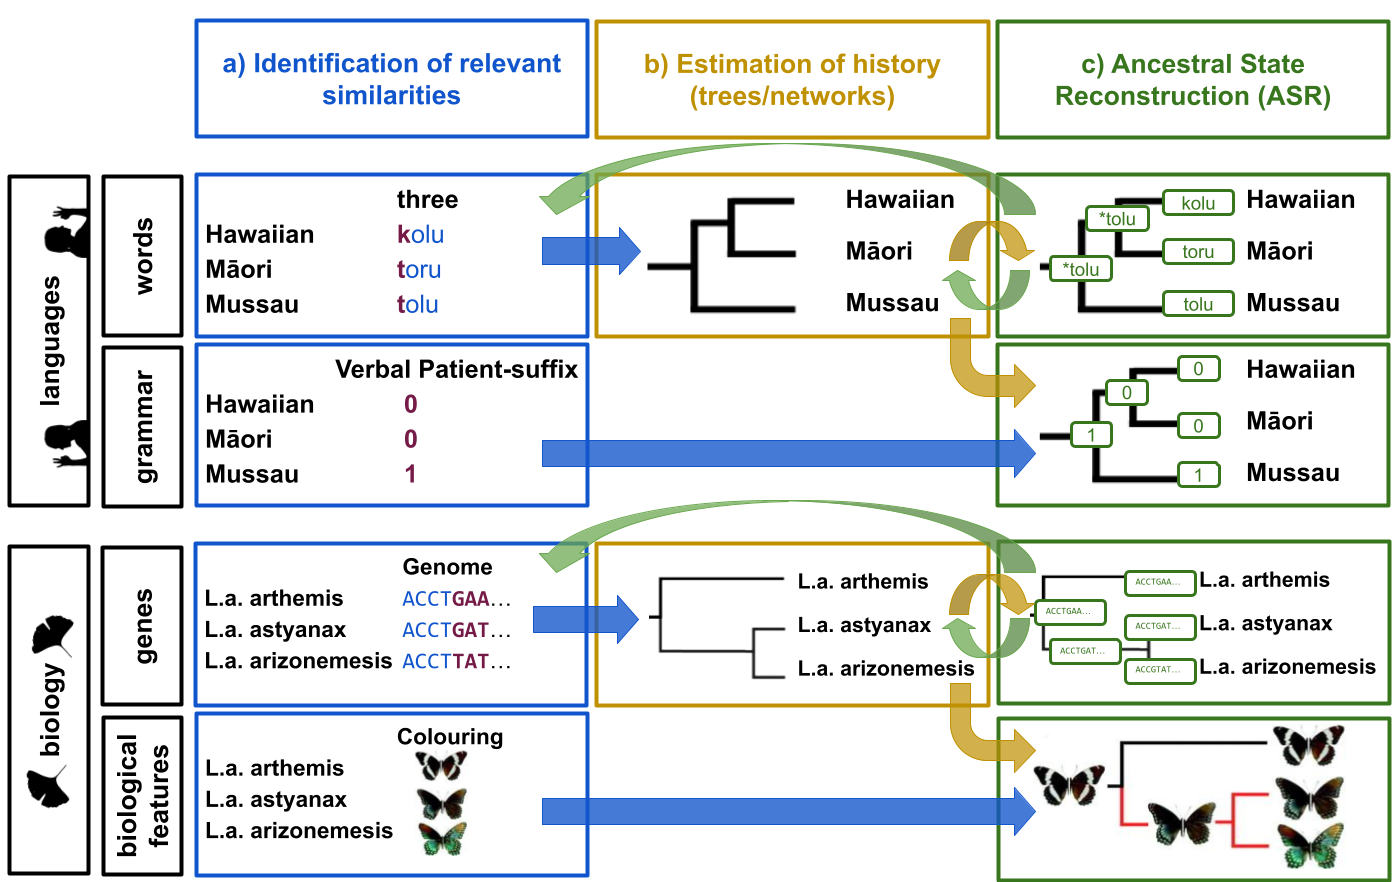
\includegraphics[width=22cm]{illustrations/ASR_HL_explainer_ill.png}
\caption{The three tasks involved in the historical reconstruction of linguistic matter (words \& sounds), patterns (grammar) and biological traits. The tasks follow each other 
The butterfly illustrations are modified from \citet{savage2009single}.}
\label{fig:HL_tasks}
\end{sidewaysfigure}

It is clear that the depth of knowledge possessed by historical linguists greatly informs their work, and that there is indeed value in linking these three tasks to each other --- for example by revising a tree when a reconstructed state does not make sense, classifying cognates of extant languages based on knowledge derived from elsewhere in the tree on how the changes can go etc. However, there are disadvantages as well. The first among these is the difficulty of providing a highly transparent methodology. This kind of labour involves a vast amount of knowledge and careful decisions, and it is not easy to make all of them explicit and accessible. 

In this paper, we focus specifically on the task of ASR --- we are not deriving new trees or re-coding structural data. In addition to increasing transparency, quantitative approaches to ASR also have the benefit of speed. If we can interrogate the conventional methods of ASR in historical linguistics and compare those principles to various computational approaches and evaluate the agreement, then we may be able to improve on transparency and offer historical linguists a convenient tool that can effectivize part of their labour.

We will be solely focusing on the third of these tasks: Ancestral State Reconstruction (ASR) and comparing the methodology and results from conventional historical linguistics to computational approaches using structural data from a large-scale typological database (Grambank v1.0, \citet{grambank_release}). 

One of the major differences between ASR in conventional historical linguistics and in biological and cultural evolution is the evaluation of appropriate data for phylogenetic analysis. Studies in historical linguistics typically require that the input data satisfies the Double Cognacy Criterion \citep{walkden_2013} --- both for the construction of trees (task b in Fig. \ref{fig:HL_tasks}) and ASR (task c). It is difficult to apply this test to non-vocabulary data because it is not clear what the correlates are to words and phonemes in structural data. 

In cultural evolution and biology on the other hand, data is deemed appropriate for historical analysis if homoplasy can be excluded. Excluding homoplasy means that it is reasonable to assume that the tree in question estimates the history of the data etc (c.f. \citet{holland2020accuracy} and \citet{evans2021uses}). One of the most common approaches to test if data is valid to use for analysis with a particular tree is to test for statistically significant phylogenetic signal. Phylogenetic signal is the \emph{tendency for related species to resemble each other more than they resemble species drawn at random} \citep[905]{blomberg2002tempo}. This concept is independent from measurements of conservatism of traits or species/languages. Tests of phylogenetic signal can be carried out for linguistic data as well as biological and cultural data, as we will learn more about in section \ref{sec:is_it_valid}.

One of the drawbacks of conventional approaches to ASR in historical linguistics is that they typically involve a great deal of manual work and, as mentioned earlier, it can be difficult to be 100\% transparent with all analytical decisions and their contexts. In particular, while there is often agreement on the presence of sound correspondences or cognate sets, there can often be conflicts regarding how to weight information and the plausibility of reconstructions. In contrast, computational phylogenetic methods are a set of tools that can be applied with great speed and all analysis is explicit and consistent even over large amounts of data. Computational approaches are not intended to replace traditional historical linguistics, but rather to function as a complement --- effectivizing parts of the process. In this paper, we compare the approaches conceptually and
examine how often computational methods of ASR arrive at the same conclusions as traditional historical linguists. We will also investigate what the computational methods say when historical linguists disagree, and make new predictions about the grammar of proto-languages.

%--- with some arguing that this cannot be included in CM at all. Furthermore,  CM produces knowledge about relevant similarity between languages (regular sound correspondences and cognates),  proto-states and sub-groupings but crucially \emph{not} branch lengths, inferences about specific migration paths etc. The methods that historical linguists use to derive this information, which is often necessary to make a language tree, is technically outside of CM ``proper''. In this paper, we will not be creating any new trees but use existing ones. However we will use methods that take into account branch lengths and compare reconstructions of abstract grammatical features specifically. The investigation goes beyond what might be called ``The Comparative Method Proper'' and concerns reconstruction in historical linguistics more generally. 

%\footnote{\citet[17-22]{clark1973aspects} is one of the more prominent instances of a historical linguists spelling out the principles underlying reconstruction in historical linguistics more generally, including syntactic reconstruction. However, 
%\citet{walkden_2013}
%} 

The practical example of this paper is the Oceanic language subgroup of the Austronesian family and the grammatical features of four of its proto-languages. We use information about the extant daughter languages from the Grambank dataset \citep{grambank_release} to infer the structure of proto-languages given three trees: a) Glottolog 4.5 \citep{glottolog4_5}, b)\citet{grayetal_2009} - MCCT and c) \citet{grayetal_2009} - 100 random posterior trees aggregate (see more in section \ref{the_trees}). 

Findings from the historical linguistics literature have been translated into data points in the Grambank format for four specific proto-languages: Proto-Oceanic, Proto-Central Pacific\footnote{The concept of Central Pacific as a coherent subgroup is not uncontroversial. \citet{grace1958position} and \citet{pawley1972internal} made a case for a subgroup consisting of Fijian, Polynesian and Rotuman. Later \citet{geraghty1996} shows that the evidence for this stage is limited. We will be using it here in this study because it occurs enough frequently in the literature, but readers should be aware that it is less likely to have been a genuine coherent language of a community compared to the others. Thank you to Andrew Pawley for drawing this to my attention.}, Proto-Polynesian and Proto-Eastern Polynesian. The computational methods take as input the language-level data points in the Oceanic subgroups and then infer grammatical states of ancestral nodes in the trees (proto-languages). The structural features of the four proto-languages are extracted for each tree and method and compared to conclusions from classical historical linguistics. 

The results are evaluated in terms of concordance between each method and the predictions from classical historical linguistics. We are evaluating how much they agree, not necessarily which one is correct. Which method is the most appropriate should be decided \emph{a priori} based on the conceptual underpinnings and assumptions of the method and how plausible that model of change is (see more in sections \ref{sec:ars:metod:hist}, \ref{sec:asr_methods} and \ref{sec:MP_ML_MC}). Both traditional methods of ASR in historical linguistics and the particular computational approaches in this paper have advantages and disadvantages. Much of the conceptual infrastructure is similar, which is why we would assume a high degree of concurrence between the methods. 

There is one area of Oceanic grammatical reconstruction where there is considerable disagreement. This concerns the nature of the alignment system of Proto-Polynesian and Proto-Central Pacific. These issues will be investigated and evaluated separately from the overall results of how much agreement there is between classical historical linguistics and computational approaches.

Finally, this study also yields predictions about grammatical features of the four proto-languages that were not addressed by the historical linguistics studies surveyed here.

%The tools of computational reconstructions are different from classical historical linguistics, and the data used in this chapter, the Grambank dataset, is different from the source material that historical linguists work with. This is further discussed in section \ref{sec:ars:metod:hist}

\FloatBarrier
\section{Background}
\label{recon_grammar}

\subsection{The methods of ASR in traditional historical linguistics}
\label{sec:ars:metod:hist}
%In order to interpret the differences between the results of the computational approach versus the classical historical linguistics approach, it is first necessary to clarify the different methodologies and their consequences. 
This section lays out the fundamental principles of historical linguistics and how they relate to this paper.

The core method by which historical linguists reconstruct language history generally is known as the ``Comparative Method''. The Comparative Method is based on finding words or morphemes in different languages that have the same (or similar enough) meaning and that display non-trivial systematic phonological correspondences. By investigating these sets of words, it is possible to deduce which are inherited from a common ancestor, i.e. which ones are so-called ``cognates''. For example, \citet{blust2004}, \citet{greenhill2011pollex} and many other scholars have analyzed M\={a}ori [maor1246] /toru/ (meaning `three') as deriving from the same word as Hawai'ian [hawa1245] /kolu/ (`three'). These two words are ``cognates'' of each other and this information can be used to reconstruct a form for proto-Polynesian. Furthermore, many words that mean the same/similar thing in M\={a}ori and Hawai'ian show this pattern of t/k, e.g. M\={a}ori: /mate/ - Hawai'ian: /make/ `to be dead' and M\={a}ori: /whitu/ - Hawai'ian: /hiku/ `seven' \citep{ABVD}. There is a systematic correspondence between these two sounds; regularly when there is a /t/ in M\={a}ori there is a /k/ in the corresponding position in Hawai'ian\footnote{Further research into more Austronesian languages shows that Hawai'ian /k/ is more likely to be an innovation and M\={a}ori /t/ a retention from an older proto-language (c.f. in the Austronesian language Amis of Taiwan `three' is /tulu/). Therefore, we can reconstruct that the change went from /t/ $\rightarrow$ /k/.}. This is known as a \emph{systematic sound correspondence}. 

One crucial part of this approach is what \citet{walkden_2013} calls the ``Double Cognacy Criterion'' which states that both the part --- the sound --- and the context it occurs in --- the word --- need to be cognate in order to form valid data for ASR and sub-grouping in conventional historical linguistics. In the above example, the sounds /t/ and /k/ are cognates of each other, as are the words /toru/ and /kolu/.

The Double Cognacy Criterion is often more difficult to apply when reconstructing structural features, which has led some to say that reconstruction of grammar is impossible (c.f. \citet{lightfoot_2002b}) and others to use a different approach which does without Double Cognacy, often labelled Syntactic Reconstruction \citep[17]{clark1973aspects}\footnote{Note that the term ``Syntactic Reconstruction'' is used for reconstruction of both morphology and syntax.}. This is relevant for the studies in historical linguistics (section \ref{sec:POC_lit_review}) that we will be comparing the computational results to. In this paper, we will compare methods of ASR in historical linguistics literature more broadly and not focus on only ASR in the specific sense of the traditional Comparative Method.

% \citep{ABVD})\footnote{Note that there are two /k/ sounds in Oceanic languages. One stems from Proto-Oceanic *t and the other from POC *k. See more details in \citet{blust2004}.}. 


%The Comparative Method provides us with a) sets of words which derive from the same word in an ancestor language (cognates), b) sequences of sound changes from proto-languages to the current observable daughter languages and c) a tree or network structure of the relationships between languages. 
%historical linguistics engage in proposing sub-groupings based on shared innovations and developing hypotheses about forms in unobserved proto-languages at the same time. 

Besides finding cognates, traditional historical linguists also propose subgroups of languages as a way of modelling their history --- typically in the form of trees. The estimation of historical relationships between languages in traditional historical linguistics is mainly/only focused on sub-grouping, which has the consequence that branch/edge lengths are typically not estimated at all. As one anonymous reviewer of this paper noted, branch length estimation is not a goal of the Comparative Method at all. This is important, because, as we will see, trees without branch lengths are most likely implausible and make for sub-optimal ASR. There is some work in traditional historical linguistics to establish branch-lengths through relative chronology of changes and archaeological anchor points (dating of clay tablets, texts etc, c.f. \citet{pereltsvaig2015indo_dates}), but that is mainly related to Indo-European. Note that estimating branch lengths need not be the same as precise chronological dating. For ASR, the key is the relative order of events rather than their precise timestamps (contrary to estimating urheimat, where dates matter more). It is also possible to incorporate uncertainty about splits - for example by positing many different trees with varying branches and splits that fit within a certain probability scope (e.g. a Bayesian posterior).

The processes of suggesting sub-grouping and ASR are done in tandem in historical linguistics; they are estimated simultaneously (c.f. \citet[7]{protooceanicvol1}
). Subgroups are proposed based on \textbf{shared innovations}. In order to determine what is and what is not an innovation, a certain amount of reconstruction of proto-languages words and sounds (ASR) is necessary. In order to do ASR, some of the tree structure needs to be approximated. The tasks are done together.

This is different from analysis in biology and cultural evolution where ASR is typically carried out as a separate next step after a reliable model of history is constructed (c.f. \citet{holland2020accuracy} \& \citet{evans2021uses}). In this paper, we are comparing specifically conventional historical approaches to ASR with computational approaches to ASR. The computational methods reviewed in this paper only does ASR, they do not suggest alternative sub-groups or trees. This makes them a bit different from classical historical linguistics approaches to ASR where sub-grouping and ASR are done simultaneously. Thankfully, this feedback loop between ASR and sub-grouping is primarily a factor in the classical historical linguistics analysis of linguistic matter (sounds and words) --- and less relevant for linguistic patterns (structural features) which is the topic of this paper.

% The computational approaches to reconstruction applied in this paper are only concerned with ASR, not sub-grouping. We are using existing trees as input, these are not estimated in themselves. 

%This is one of several differences between the computational reconstruction methods and conventional approaches in classical historical linguistics.
%we are only focussing on the reconstruction --- not on the identification of regular sound correspondences, cognates or subgroups. 


%list the reconstruction */gaawari/ for Proto-Polynesian as meaning `weak, feeble'. In some of the daughter languages, words deriving from this Proto-word are listed as meaning `bent', `weak', `soft' and `slack (of man)'. These meanings are judged to be plausible semantic extensions of the proto-meaning such that they can be said to be related ---- to be cognates. 

%\footnote{In order to estimate what semantic shifts are reasonable, linguists can study colexifications in contemporary languages. These are instances of different meanings that are expressed by the same word. In the Database of Cross-Linguistic Colexifications (CLICS), users can explore clusters of colexifications, for example: the concept ``sun'' is more closely linked to ``day (not night)'' than it is linked to ``name'' ) \cite{list2018clics2}.}

Historical linguistics has been primarily concerned with the reconstruction of sounds and words, but there is also work on the reconstruction of grammatical features such as morphemes or word order. \citet[17-22]{clark1973aspects} outlined three general principles for ASR in traditional historical linguistics that can be applied to structural data and vocabulary\footnote{It is also possible to include information on the history of particular regions and cultural factors when conducting linguistic ASR, but this is less often made explicit. In the case of Indo-European, which is the language family that has received the most attention so far in historical linguistics, there are even specific procedures involving particular parts of the tree. For example, \citet[6]{goldstein_2022} describes the ``Anatolian Criterion'' whereby ``Proto-Indo-European ancestry can only be established for cognate sets that include an Anatolian language''. This is because most historical linguists working on Indo-European see Anatolian languages as an early off-shoot branch of proto-Indo-European. In addition, work on the Indo-European language family can also make use of explicit information on ancient languages where we do have textual remains, such as Latin, Sanskrit etc. These kinds of procedures are currently not available for most language families in the world, historical linguists working on Indo-European represent a particularly privileged position informationally in relation to the field at large.}:

\begin{enumerate}[label=(\roman*)]
\item the number of changes posited (as few as possible, also known as Maximum Parsimony)
\item the plausibility of the changes posited
\item the plausibility of the reconstructed language as a human language (i.e. the degree to which the reconstructed traits work well in harmony with each other)
\end{enumerate}

%As was highlighted earlier, ASR in historical linguistics is part of the overall toolbox of the Comparative Method, and as such is done simultaneously with the other two tasks. In this paper, we will be comparing specifically ASR of historical linguistics to computational approaches to ASR.

%The Comparative Method (CM) is a set of principles that can be applied to a set of languages and data to derive sub-groupings and ancestral states  This approach has yielded great results, such as the inference of many language families and proto-languages, and has robust control for avoiding trivial similarities. In addition, historical linguists also apply a similar approach to the historical analysis of structural features such as morphology or syntax (e.g.\citet{harris2008reconstruction} \& \citet{walkden_2013}). Historical analysis of patterns (structural features) is less common and more controversial than the reconstruction of matter (sounds and words), primarily because it is difficult to apply the rigorous criteria whereby something is defined as a cognate to structural features \citep{walkden_2013}. This problem has led some scholars to label the enterprise Syntactic Reconstruction rather than incorporate the exercise as an application of the Comparative method \emph{per se}. In this paper, we will be comparing the reconstructions of patterns made by classical historical linguists to the outcomes of computational approaches to ASR that takes as its input abstract typological features. To make it clear that we are focussing specifically on ASR and not the Comparative Method overall we will use the term ASR throughout the paper.

%\begin{enumerate}[label=(\roman*)]
%\item the number of changes posited
%\item the plausibility of the changes posited
%\item the plausibility of the reconstructed language as a human language (i.e. the degree to which the reconstructed traits work well in harmony with each other)
%\end{enumerate}

The first of these principles (``fewest amount of changes'') is the same as what is known in the wider field of phylogenetics as ``Maximum Parsimony'' \citep{felsenstein2004inferring}. The idea is to reconstruct states in proto-languages such that there are as few changes as possible between nodes in the entire tree. \citet[17-22]{clark1973aspects} explains how this works by positing an example of seven languages where there is a majority of one kind of value, X, and fewer of another, Y. Fig.~\ref{fig:clark_tree} illustrates this example. If we only examine which feature is the most common, we should reconstruct X at the root of this tree (this is what \cite{goldstein_2022} calls the ``frequency heuristic''). However, this candidate solution would result in two changes (one each on the two paths from the root and to tips A and B respectively). If we instead reconstruct Y at the root, we would only need one change (between the root and PC-G). The solution where we reconstruct Y at the root results in fewer changes --- it is the most parsimonious --- and is therefore the preferred candidate.
 
\begin{figure}[ht]
\centering
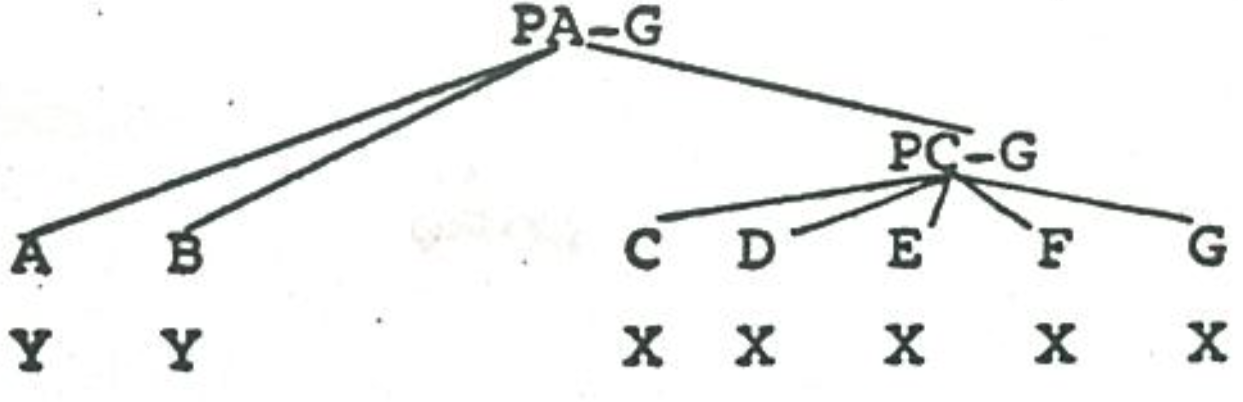
\includegraphics[width=8cm]{illustrations/Clark_1977_tree.png}
\caption{{Tree from \citet[19]{clark1973aspects} illustrating Maximum Parsimony.}}
\label{fig:clark_tree}
\end{figure}

It is important to note that Maximum Parsimony does not take into account the length of branches, only the changes between each node of the tree (regardless of how far apart they are). It is of course possible that the true solution is \textit{not} the one with the fewest changes. Maximum Likelihood (and other more recent ASR methods) improve upon this by taking branch lengths into account and actively estimating likely asymmetric rates (the rate of change X$\rightarrow$Y can be different from Y$\rightarrow$X) and actively applying the most likely rate to the inference of unknown ancestral states. ML attempts to find the most likely solution, MP can be said to find the solution with the slowest rate\footnote{It should be noted that my use here of ``rate of change'' in relation to Maximum Parsimony (changes per branch) is not directly comparable to rates of change estimated by other methods, such as ML. MP does not technically estimate a rate of change at all and does not model branches in a meaningful way, it is only concerned with changes between nodes. MP can however be said to \emph{assume} the slowest rate of change, given the definition of the rate as ``changes per branch''.}.

The next principle of ASR in historical linguistics concern the plausibility of changes --- phonological, semantic or grammatical. For example, many historical linguists posit that /s/ is more likely to become /h/ than it is to become /k/\footnote{Historical linguists do concede that there are instances of irregular sound change \citep{blust1996neogrammarian, campbell1996sound} and that while they can often be explained by contact, analogy or avoidance of homophony, they sometimes remain unexplained.} and this information is taken into account when doing ASR. Going to semantics next, in the earlier example from M\={a}ori and Hawai'ian, the words /toru/ and /kolu/ both mean `three', but it is possible for cognates to have less similar meanings. For example, \citet{pawley2005meaning} reconstructs the proto-form *\emph{panua} as meaning `land' or `inhabited territory'. In various daughter languages, this has changed to `place', `community', `village', `house', `people', `world' and `weather'. The meanings are related to each other, but not identical as in the 'three' - 'three' example earlier. Historical linguists aim to find plausible semantic connections between words that are proposed to stem from the same proto-form, they cannot be too dissimilar. The sound correspondences can be guiding here, if two forms have somewhat different meanings but convincing sound correspondences then they may still be cognates. This is difficult, as can be seen from this quote from \citet[229]{anttila1989historical}: \emph{there are no exact rules for handling semantic change; the final factor here is necessarily the common sense and the experience of the individual scholar}. 

The plausibility of changes also comes into play when reconstructing structural traits. For example, a language going from having no marked dual number on nouns to having a trial number category would be taken as unusual by most linguists \citep[c.f.][8]{kikusawa_2006_pro_number} --- it seems like the language has skipped over a necessary step, jumping from `many' directly to `three' without passing `two'. Grammaticalization theories have given rise to a number of these plausible historical changes \citep[594-5, 598]{heine2003grammaticalization}.

Lastly, ASR in historical linguistics deals with the plausibility of the whole of the reconstructed proto-language as a system \citep[1]{clark1973aspects}. For example, if we reconstruct a language with very uncommon combinations of features we should be wary and probably question the analysis. For example, it is rare to find a language that has a gender distinction in the first person, but not in the third (though not impossible; c.f. \citet{wals-44}). If the solution results in a proto-language with many rare features or unusual combinations of features, the work may require reconsideration. If something is rare in the languages that exist today, we would expect it to be relatively rare also in past languages. This is more relevant for phonology and linguistic structure where we have more worked-out theories of plausible combinations than in the lexicon. This principle has parallels in biology as well, where they avoid impossible ancestral states (c.f. \citep{schulmeister2004comparative}).

The procedure of ASR in historical linguistics that has been outlined in this section can and has been applied successfully to sounds and words (be they lexical or grammatical words). The application of this approach to abstract structural features is more controversial, and is not always included under a more strict application of the term ``Comparative Method'' \emph{per se}. For this reason, we will refer to ``traditional historical linguistics ASR'' rather than the ``Comparative Method'' in relation to bodies of work that concern the reconstruction of the grammar of proto-languages (see section \ref{sec:POC_lit_review}). It is notable that most of the discussion regarding whether structural ASR is possible has been in relation to Indo-European languages (c.f. \cite{walkden_2013}). This paper offers a view from the Pacific Ocean, where the waves of the debate are more peaceful.

%See more in section \ref{sec:is_it_valid}.

%. We cannot compare Parsimony cost directly to rate of change estimated by other models, but out of all the possible solutions Maximum Likelihood generates it does not necessarily select the one with the slowest rate of change  (more on this in section \ref{sec:asr_methods}).


%harris2008reconstruction


%As a consequence of that, it can be said that not all reconstruction in historical linguistics is based on the Comparative Method in a strict sense.. Some of the work on reconstruction in historical linguistics cited in this paper can be said to represent \emph{traditional approaches}, but perhaps not necessarily the \emph{Comparative Method} in a strict sense.

%{\color{red}This section and section \ref{diff_lexi_str} are being re-written to more clearly tease out and discuss details of reconstruction of abstract structural features.}

%The plausibility of the reconstruction language to be a human language relies on knowledge about which traits are likely to go together, and which would represent a combination that is veyr implausible. For example, if a language has a dual number category for nouns, i.e. signalling that the number of items is 2, it is likely to also have general plural number. If a reconstruction produces a language with a dual but not a plural, this is cause for concern as this is very unlikely according to linguists. The same is true of the plausibility of the changes from state to state themselves, some changes are assumed to be more frequent and common than others. However, linguists rarely spell out all of these assumptions explicitly in historical reconstruction, which makes it hard to evaluate what is happening. It also makes it difficult to incorporate these concepts in computational reconstruction. 

%Integral to the reconstruction of forms in historical linguistics is \textbf{Maximum Parsimony}. Maximum Parsimony is a method of reconstruction ancestral states (in this case grammatical features of proto-languages) in such a way that there is as few changes as possible from the root to every tip (language). 

\FloatBarrier
\subsubsection{Disagreements in historical linguistics}
\label{sec:hl_disagreements}
As discussed, ASR in historical linguistics includes judgements of plausibility. This requires some assumptions about what are plausible features to co-occur in language, and which pathways of language change are more plausible than others. 

Plausibility is important for ASR, both in linguistics, cultural studies and biology. However, this principle is sensitive to differing assumptions and theories. What is more plausible as a reconstructed language, society or species may differ from scholar to scholar. Besides debates over precise sub-groupings, many arguments in historical linguistics boil down to disagreements about the plausibility of combinations of traits or of changes. This is also true of the different reconstructions of the alignment system of Proto-Polynesian.

\citet{clark1973aspects} disagrees with \citet{hale_1968}, \citet{hohepa_1969}, and \citet{chung1978} on the case-marking systems of Proto-Polynesian on grounds of plausibility. Chung, Hale and Hohepa argue for a reconstruction that is technically less parsimonious on most trees of the languages (i.e. involves more changes), but which they say is more plausible. They posit that Proto-Polynesian had a nominative-accusative case marking system\footnote{Hale, Hohepa and Chung actually suggest three different theories which differ in specific details. For a summary of the differences between the proposals, see \citet[247-249]{chung1978}.}. If this was the case, that would mean positing more changes along the tree than if we assumed, as \citet{clark1973aspects} does, that the Proto-Polynesian language was ergative-absolutive. This is due to S\={a}moan and Tongan both having ergative-absolutive marking and both splitting off early (in most accounts of the Polynesian tree) from Proto-Polynesian. Fig. \ref{poly_GB409_tree} shows the Polynesian tree with Grambank feature GB409 values marked out\footnote{Grambank feature GB409 asks if \emph{any} ergative flagging is present. In some instances, the system is not wholly or primarily ergative, but ergative marking is present. It is possible that the scholars involved in the debate would not classify such languages as ``ergative-absolute'' languages \emph{per se}.}.

\begin{figure}[p]
\centering
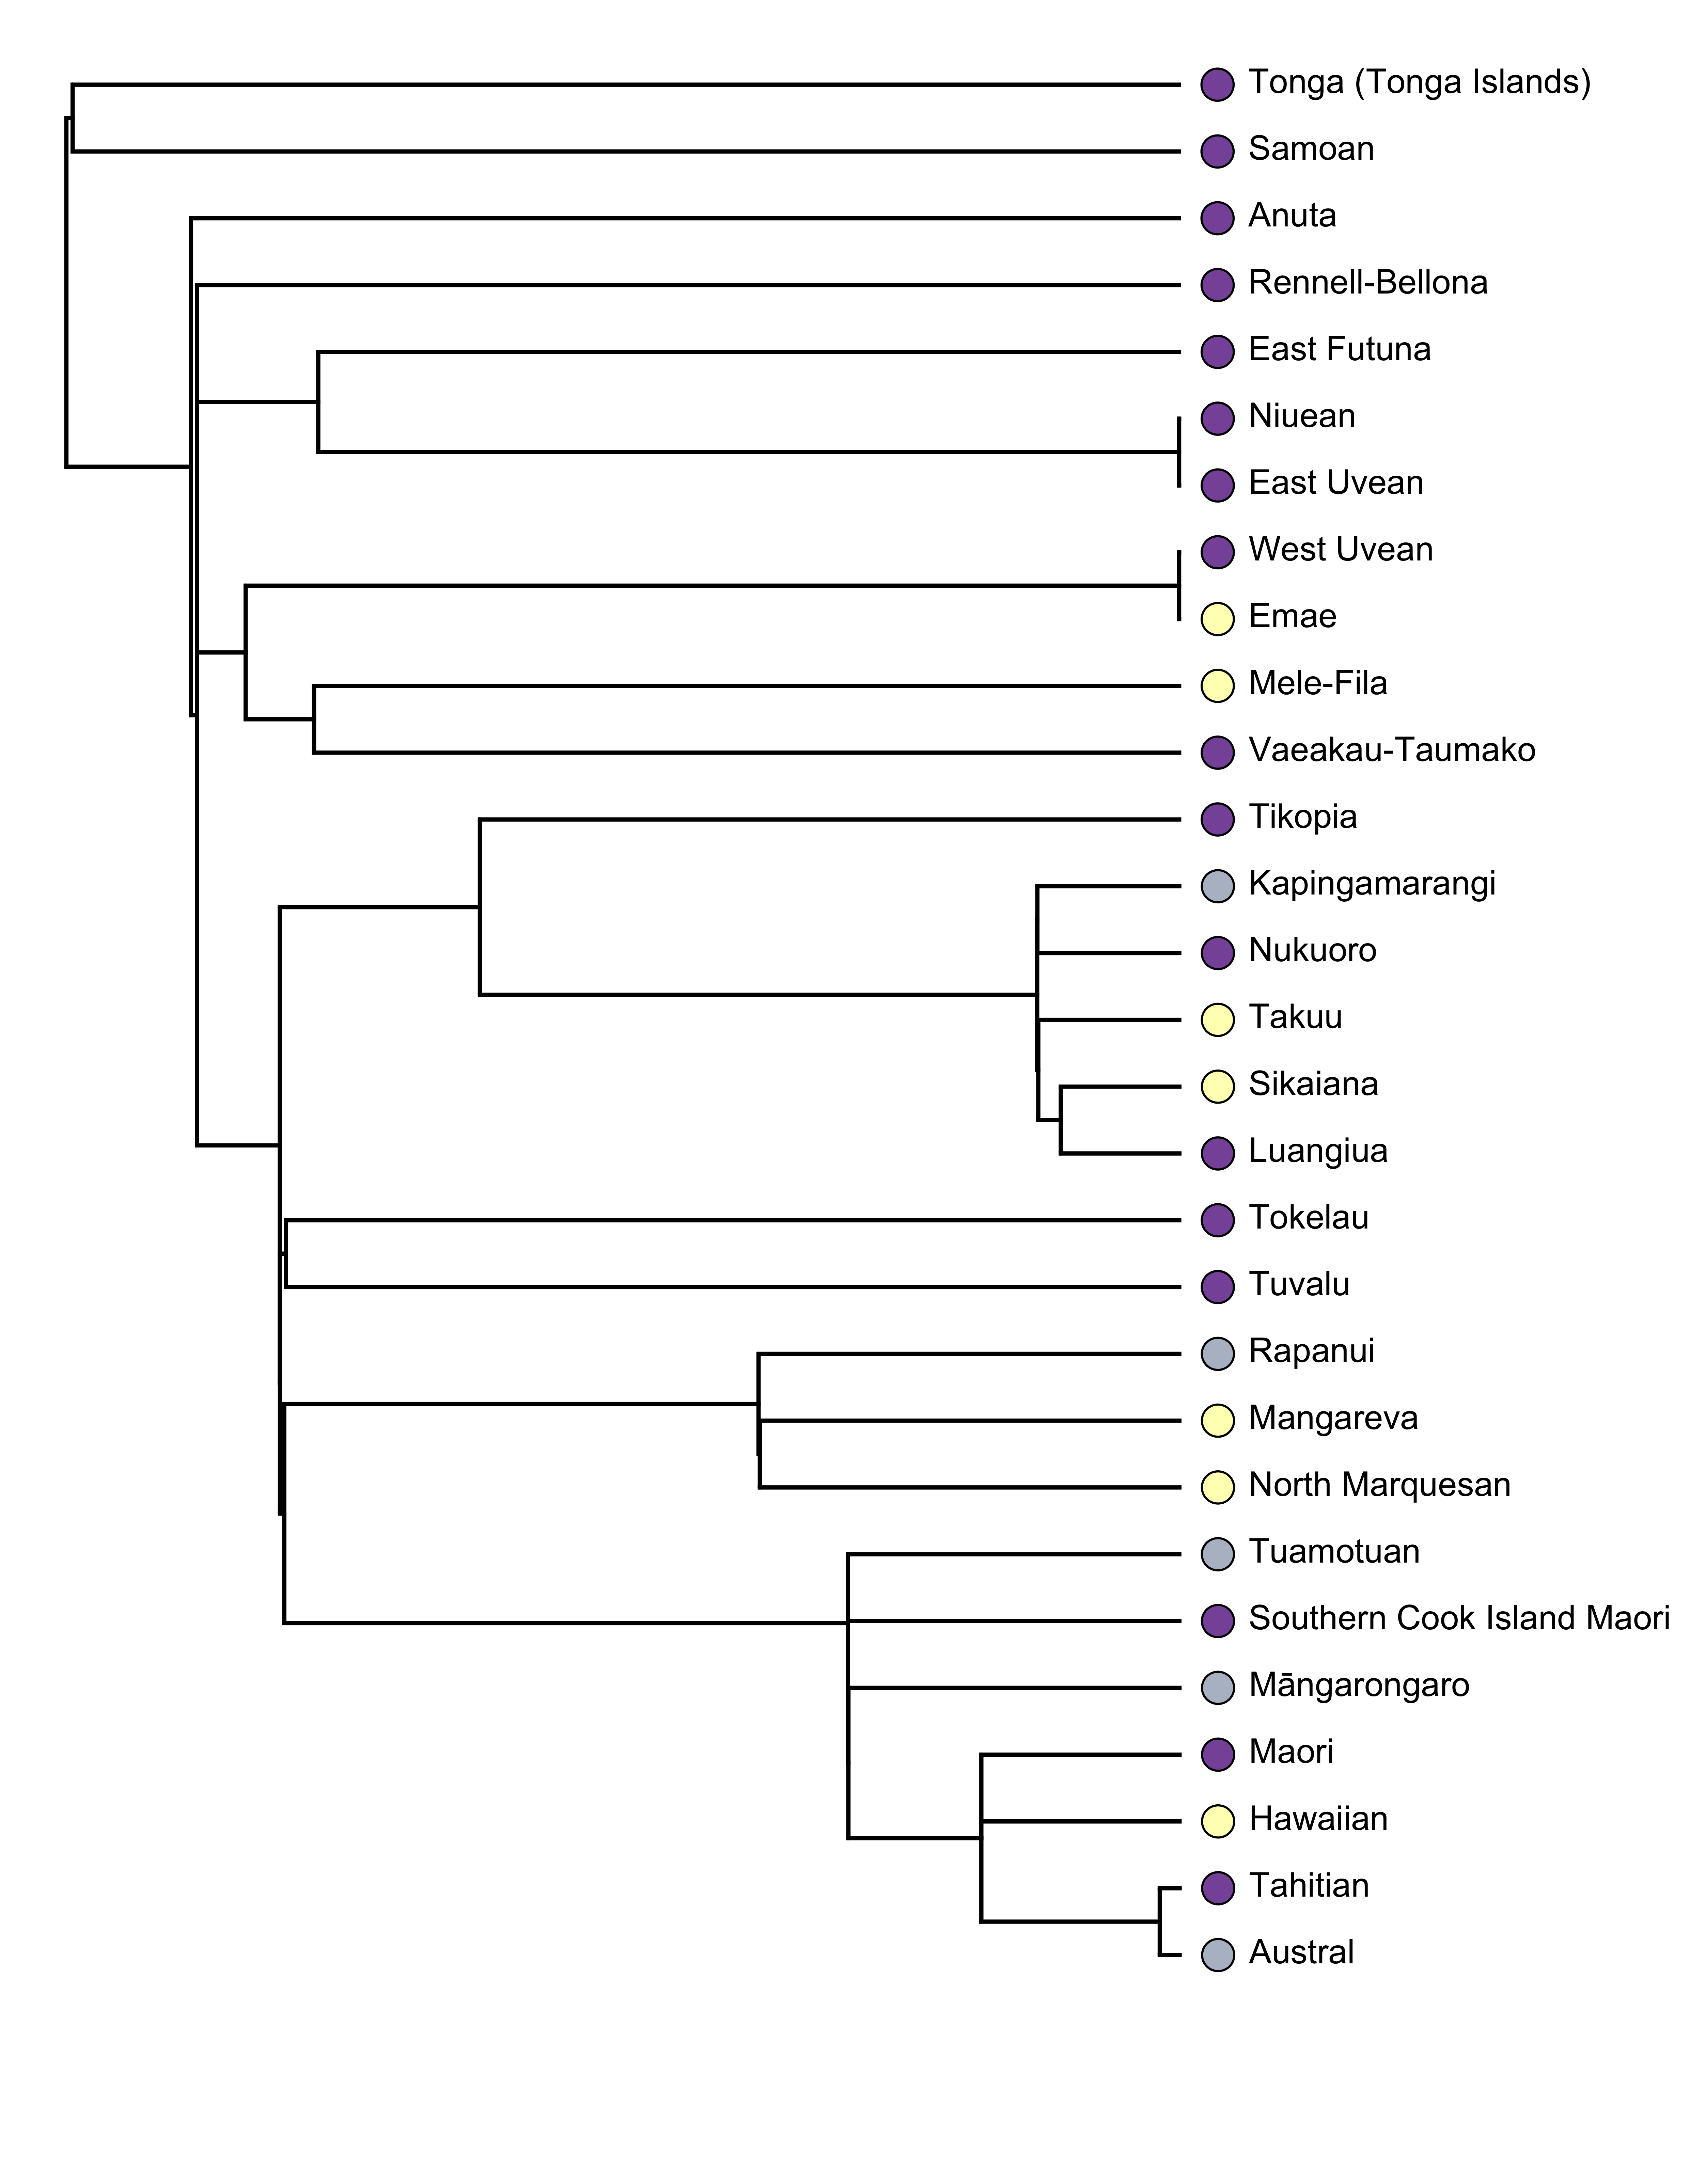
\includegraphics[width=16cm]{illustrations/plots_from_R//tree_plots/poly_tree_example.png}
\caption{{The Polynesian languages in the \citet{grayetal_2009} Maximum Clade Credibility Tree-tree, with the coding of Grambank feature GB409 ``Is there any ergative alignment of flagging?'' marked out. Purple = Yes, Green = No and absence of dot = Not enough information/not clear.}}
\label{poly_GB409_tree}
\end{figure} 

I have summarised Chung's critique of Clark's proposal into three main points:
 
\begin{enumerate}[label=(\alph*)]
\item the tree used is not an accurate representation of the language history (there was more interaction between S\={a}moan and Tongan after splitting, and these interactions explains the situation)
\item it is possible that the Proto-language contained variation and was undergoing change that was only fully realised in some of the daughters
\item the morpho-syntactical historical process itself is less plausible
\end{enumerate}

In a review of \citet{clark1973aspects}, Chung writes:

\begin{quotation}
\noindent\emph{Such an approach} [as Clark's] \emph{relies on the assumption that the subgroups have developed quite independently once they split off from Proto-Polynesian, so that features shared by both must be attributed to the Proto-language. But in fact, both parts of this assumption are too strong. It is well known that the two primary subgroups of Polynesian did not develop totally separately; there was long-standing contact in pre-European times between speakers of Tongic and some Samoic-Outlier languages, as Clark himself notes (p. 27). Further, and more generally, it is simply not true that every feature shared by related languages must have existed in the Proto-language uniting them. Languages are constantly undergoing change; it is reasonable to suppose that Proto-languages were no different from real languages in this respect. But if this is so, then it is also reasonable that changes begun in a Proto-language may have continued even after its separation into daughter languages. In this way, related languages may come to share a feature that existed only in embryonic form, or not at all, in their common ancestor.}
\end{quotation}
\begin{flushright} \citet[539]{chung1977aspects}  \end{flushright}

This debate contains more twists and turns, with each side arguing for the plausibility of their account. In our analysis, we will be using trees that represent the history of the languages in a similar way to Clark, which means the results are sensitive to the same critique by Chung (i.e. not taking into account contact between S\={a}moan and Tongan). We are also not able to use plausibility in our computational reconstructions since we do not have access to formalised data on what plausible language profiles or changes are. This is a key difference between computational reconstruction and traditional approaches to reconstruction. Knowledge of plausibility and how to weigh different kinds of evidence against each other is not formalised and therefore cannot be taken into account.

%It is possible that with the added information on rates of change and branch length that comes with the Maximum Likelihood approach we are able to approximate some parts of historical linguists' knowledge of plausibility. In that case, we would expect the Maximum Likelihood results to concur more with the predictions by expert linguists. If historical linguists mainly do operate on the same principles of Maximum Parsimony, and/or Maximum Likelihood is not able to approximate plausibility, we would expect the results of Maximum Parsimony to concur more with findings in traditional historical linguistics.

In this study, any instances of conflicting data from historical linguists concerning proto-languages are evaluated separately from the overall results and will be reported in a separate section. There are three instances of this: two features related to the alignment of Proto-Polynesian (GB408 Is there any accusative alignment of flagging? and GB409: Is there any ergative alignment of flagging?) and one feature for Proto-Central Pacific, where \citet{kikusawa2002proto} and \citet{ball2007ergativity} disagree on the alignment as well.

%can fall short of reconstructions carried out by classical historical linguists because they are able to take these plausibility considerations into account.

%\subsubsection{Reconstruction and sub-grouping in tandem}
%The processes of sub-grouping and reconstruction are done in tandem in historical linguistics; they are estimated simultaneously. Subgroups are proposed based on shared innovations. In order to determine what is and what is not an innovation, a certain amount of reconstruction is necessary. In order to make reconstructions, some of the tree structure needs to be approximated. Pawley (personal correspondence) notes that most of the sub-grouping done in historical linguistics tends to be at the lower level. 
%This can be seen later in this paper in the difference between the Glottolog tree (Fig. \ref{tree_coverage_oceanic_glottolog}), which is based on classical historical linguistics,  and the Gray et al 2009-tree (Fig. \ref{tree_coverage_oceanic_gray}), which is inferred with Bayesian phylogenetic methods using basic vocabulary data. Most of the splits in the Glottolog tree occur close to the tips, whereas the splits are more spread out over the distance between the root and the tips in the Gray et al 2009-tree.

%Besides parsimony and plausibility, it is also important to know how to weight evidence when conducting historical linguistics research, in particular when it comes to sub-grouping. This is less often discussed explicitly, but it is related to issues of plausibility and is likewise a source of disagreement. It is for example possible that certain data-points are more susceptible to contact-induced change than others, and should therefore carry less weight if we are trying to infer a family tree. This is why items and features that are thought to be particularly stable and unlikely to be borrowed are used in reconstruction and sub-grouping \citep[c.f.][]{pawley_2009_solomons}.

%In this paper we are not proposing any new sub-groupings, so the problem of weighting evidence is not present in this manner. For the reconstruction of grammatical features, all languages are weighted as equally valuable and we use the tree topologies directly to control for non-independence of datapoints as opposed to careful sampling \citep[c.f.][]{ross2004morphosyntactic}.
%We are reconstructing grammatical features and this is another area where weighting can be relevant. All languages are weighted the same for the reconstruction, but 

%As was discussed in \ref{sec:dep}, not all data-points are independent of each other and this may be one reason to weight them differently. 

%For example, \citet{wilson_whence} presents a case for Eastern Polynesia (EP) being settled from the so-called ``Northern Outliers'' (i.e. Polynesian languages of Micronesia and the Solomons) by demonstrating shared innovations of lexicon and grammar to the exclusion of Samoa, Pukapuka and Tokelau (which were closer to EP in previous proposals). The paper lays out 73 innovations in support for this theory, and states that there is a lack of shared innovations supporting grouping Eastern Polynesia and the Samoic group together, as had been previously suggested by \citet{pawley1966polynesian}. \citet{wilson_whence} proposes that a more accurate reflection of this data is to group Eastern Polynesian with the Northern Outliers. On the other hand, \citet[53, 61]{pawley1966polynesian} presents two cases where Samoan and some of the Northern outliers shared features to the exclusion of Eastern Polynesia (sing/plural distinctions in indefinite articles and the form of the human number prefix). Besides the sheer number of data-points, it is clear that historical linguists also weight different pieces of information differently. Without an internalised in-depth knowledge of these matters, it is difficult to know how to evaluate the support for these conflicting theories of the origins of Eastern Polynesian communities. Is it as significant that the Northern Outliers and Eastern Polynesian languages shared a word for a certain kind of fish (\emph{*kamakama}) as the fact that they have also, as a group, added an \emph{o-} to the Proto-Polynesian root \emph{*fia} (want) \citep{wilson_whence}? 

%In this paper we are not proposing any new sub-groupings, so the problem of weighting evidence is not present in this manner. We are, however, reconstructing grammatical features and this is another area where weighting can be relevant. All languages are weighted the same for the reconstruction, but 

%The tree structure and the method (Maximum Parsimony or Maximum Likelihood) determines the reconstruction. This can be compared to weighting evidence from oversampled areas/subgroups less when reconstructing. 

% \citet[135]{marck2000} also presents the case that the Northern Outliers are most closely related to Tuvaluan.

%It is clear that considerable experience and meticulous considerations are needed in order to make these judgements and interpret the results of these papers appropriately. This entails long periods of training and familiarisation with the method in practice and the particular languages in question. \citet[721-731]{blust2013austronesian} suggests that we should bring in non-linguistic evidence to bear on these theories as well. How would a settlement from the Northern Outliers be achieved materially? By finding supporting or conflicting evidence from other disciplines, we can make more robust predictions 

%For full disclosure, both of the trees used in this study (Glottolog 4.5 and \citet{grayetal_2009}) group EP closer to the Northern Outliers than to Samoan, and it is becoming more accepted. 


%Each of these tasks can be accomplished by different approaches. For example, historical linguists have certain criteria regarding what qualifies as relevant units to compare over (task a) and what ends up underlying the construction of the history (task b). In contrast, biologists use many different kinds of methods for Ancestral State Reconstruction: Maximum Likelihood, Stochastic Character Mapping etc (c.f. \cite{joy2016ancestral}), not to mention the variation in tree-constructing methodology. 

\FloatBarrier
\subsection{Evaluating if the data is valid for phylogenetic analysis: the Double Cognacy Criterion and phylogenetic signal}
\label{sec:is_it_valid}

There is considerable debate within historical linguistics regarding if patterns (grammar) can indeed be analysed with the Comparative Method at all. One if the primary sources of disagreement is the criteria whereby similarities are judged to be valid for historical study. The Comparative Method is built on the recognition of the importance of cognates and sound correspondences --- two concepts that are difficult to translate into the world of morphology and syntax (see for example \citet{harris2008reconstruction} \& \citet{walkden_2013}). In order to establish shared inheritance, two languages need to exhibit pairs of words where the words themselves can with great certainty be said to be related and where there is also a correspondence between the sounds \emph{within} the words. This is what \citet{walkden_2013} calls the ``Double Cognacy Condition''. What does this mean for grammar? Are morphological patterns within sentences similar to sounds within words? The answer is not clear, and most likely varies depending on what kind of structural data we are dealing with (word order vs organisation of pronoun paradigms vs presence of certain markers etc). For this study, we will not delve too far into this debate but instead, use a quantitative test of phylogenetic signal to estimate if the data is suitable for ASR.

%For the four proto-languages and structural traits considered here, 118 data-points are described in the classical historical linguistics literature (see \ref{sec:POC_lit_review}). In contrast, the computational approaches derived an additional 686 predictions about structural features of long-gone languages. 

We take a leaf out of the books of cultural evolution and biology in terms of evaluating if the data is appropriate for phylogenetic analysis. In these fields, the three tasks outlined earlier are separated out; appropriate data for analysis is collected (this can differ for tree/network construction and ASR) and trees\footnote{History of organisms and culture can be understood as trees, waves and networks. For the sake of space, we will write ``tree'' since this is most common but waves and networks are not excluded \emph{a priori}.} are constructed (usually with carefully chosen model approaches and priors). Once a reliable tree exists, ASR is carried out as a separate next step (c.f. \citet{holland2020accuracy} \& \citet{evans2021uses}). There is a veritable smörgåsbord of methods that a scientist can choose to apply to each task. For example, you can use a plain distances-based approach to making a tree \citep{jager2016inferring} or engage with more sophisticated Bayesian tools like BEAST \citep{drummond2015bayesian}. Similarly, for ASR there are different approaches with different pros and cons (see \cite{joy2016ancestral} for an overview). 

The input data for ASR can differ from what was originally underlying the construction of the tree. If we believe that the tree is likely to be a good estimation of the history also for other data besides what it was directly based on, we may be able to carry out analysis with that tree on different data. For example, \citet{watts2016ritual} analyzes evolutionary dynamics of societal variables such as ritual human sacrifice and social stratification in the Pacific using trees that are based on basic vocabulary and archaeological priors of island settlement \citep{grayetal_2009}. Besides arguing that it is reasonable to assume that the history of a community's sociopolitical past is similar to its linguistic past, we can also test the strength of the phylogenetic signal statistically and use this as a guide. If the data has a reasonable phylogenetic signal, we assume that it is likely that it was generated by the tree and that we can proceed with further analysis. This is what \citet{watts2016ritual} did for their data, and they found that it was possible to carry out the analysis. We can do this as well for our Oceanic trees and structural data.

% Some scholars even state ASR of structural features is impossible \citep[c.f]{lightfoot_2002b}. One of the concerns is whether the underlying data represents genuine correspondences (for example by satisfying the Double Cognacy Condition as described by \citet{walkden_2013}). \citet{walkden_2013}) explores the possibility of successful reconstruction of a structural feature and outlines that one possible approach is to break down structural patterns/item into definitional features (similar to phonological features) and consider syntactical context as similar to phonological context (words). For this study, we are using Grambank features which are accompanied by coding documentation that shares certain similarity to the features Walkden describes...

%<insert more on walkdens similarities to \citet{traugott2003constructions} and\citet{heine2003grammaticalization} >

Phylogenetic signal is the degree to which it can be assumed that a particular tree is likely to have given rise to the data in question, the tendency of related tips to resemble each other more for a particular variable than they would if randomly re-arranged\footnote{Nota bene: this is \emph{not} the same as stability/conservatism, phylogenetic signal is a separate concept.}\citep[905]{blomberg2002tempo}. There exist several different tests of phylogenetic signal, among others: Pagel's $\lambda$ \citep{pagel1999inferring}, Bloomberg's K \citep{blomberg2003testing}, Borges et al's $\delta$ \citep{borges2019measuring} and Ives \& Garland's alpha \citep{ives2010phylogenetic}. In this study we will use a common and conceptually simple measure: \citet{fritz2010selectivity}'s \emph{D}-estimation. This metric has been used in language studies on sounds of languages \citep{macklin2021phylogenetic} and grammatical features \citep{hubler2022phylogenetic} and is relatively straightforward. The D-algorithm takes a tree and a binary trait (in this case structural linguistic features) and simulates what the distribution of values would be if the data was a) generated by Brownian evolution or b) randomly generated. Both scenarios are simulated with the same prevalence of tip states as the real data. The algorithm produces a D-estimate for each trait and tree, which represents the similarity to these two scenarios. If this value is close to 1, the data is similar to what would happen if the data was randomly generated (if the D-metric is higher than 1, this represents it being over-dispersed\footnote{Over-dispersed here means that the trait is spread out over the tips in a way that shows no clusters, even less clustered than one might expect by chance. For example, sister-pairs may have opposite values to each other all throughout the tree. See table 1 in \cite[1044]{fritz2010selectivity} for illustrative figures.}) and if it is near 0 then it is more similar to Brownian evolution. The algorithm also produces conventional p-values which show how likely it is that the data is dissimilar from 0 (Brownian) and 1 (random). The conventional p-values are practical because they take into account sample size. 

In this study, we are primarily concerned with 84 unique Grambank features \footnote{Sometimes we are interested in the same feature for more than one proto-language. The total amount of data points we are interested in for comparison to conventional historical linguistics is 115, which reduces to 84 specific unique features.} and three trees (Glottolog 4.5 \citep{glottolog4_5}, \citet{grayetal_2009}-MCCT and an aggregate of 100 random trees in the \citet{grayetal_2009} posterior). We carried out the D-estimate analysis on all of these features over all trees using the function phylo.d in the R package caper \citep{orme2013caper}. The results are summarised in table \ref{d_estimate_summary}. The second column of the table shows the mean D-estimate value over all 84 relevant Grambank features for each phylogeny. The third column shows the percentage of features with p-values that indicate that they are similar to 0 (p < 0.05), i.e. similar to Brownian evolution. The fourth column shows the number of features for which it was not possible to carry out the D-estimate calculation because they do not meet the rigours of the model. In all of these cases, it was because there was a very skewed distribution of values over the tips (e.g. 4 tips with ``absence'' and 118 with ``presence''\footnote{It does not matter here whether it is the presence or absence of a trait that is rare, this has no effect on the measurement of phylogenetic signal.}) and this is not suitable for the analysis (for more technical details see Supplementary Material \ref{supp:d_estimate}). We can consider all of these to be a kind of ``super-conservative'' (the feature rarely evolves), but we cannot derive a measurement of phylogenetic signal \emph{per se}. Lastly, some features were excluded because there was too much missing data which caused the pruned trees to have too few tips.

% latex table generated in R 4.2.2 by xtable 1.8-4 package
% Wed Mar 15 19:45:54 2023
\begin{table}[ht]
\centering
\begin{tabular}{p{5cm}p{3cm}p{3.5cm}p{3.5cm}p{3.5cm}}
  \hline
tree & D-estimate (mean) & Proportion of features signficantly similar to 0 & Too few tips in minority state & Too few tips altogether \\ 
  \hline
glottolog & 0.26 & 51\% &  17 & 13.00 \\ 
  Gray (2009) - mcct & 0.45 & 62\% &  22 & 16.00 \\ 
  Gray (2009) - posteriors & 0.14 & 89\% &  33 & 16.00 \\ 
   \hline
\end{tabular}
\caption{Table showing D-estimate (phylogenetic signal) of Grambank features that map onto research in traditional historical linguistics.} 
\label{d_estimate_summary}
\end{table}


Most features under study have a D-estimate similar to 0, meaning that they have phylogenetic signal. There is however many features that are not similar to a D-estimate of 0. The results and conclusions further discuss the relationship between this principle and agreement with conventional HL.

 
%While it is true that reconstruction of structural features is not the same as reconstruction of lexical items and sounds, several scholars have found that it is achievable. Most of the discussion of particular reconstructions and theoretical matters have been in relation to Indo-European languages. In this paper, we turn to the traditions and achievements in Oceanic linguistics in particular. We can be heartened by several publications on the reconstruction of grammatical features in Oceanic (see section \ref{sec:POC_lit_review}), but we can also substantiate the validity of this enterprise by investigating the phylogenetic signal of Grambank features. Grambank features are binary, and therefore we use the D-estimate approach from \citet{fritz2010selectivity} to estimate phylogenetic signal. If there is phylogenetic signal in Grambank data for Oceanic languages, that is an indication that reconstruction can be fruitful. D-estimates are singular numbers, if they are close to 0 then the given feature behaves similarly to Brownian evolution, if it is closer to 1 it is more similar to random evolution (no phylogenetic signal). Values can also be higher than 1 (overdispersed) and lower than 0 (more conserved than Brownian evolution). See Supplementary Section \ref{supp:d_estimate} for more tehnical details on D-estimates. For this study, we use 3 different trees: Glottolog, Gray et al 2009-MCCT and an average over 100 randomly selected posterior trees of Gray et al 2009. The table below shows the average D-estimate for all features per tree. The D-estimate test also determines a p-value of how different the D-estimate is to 0, the third column in the table shows the proportions of features per tree that are similar to 0 (given a cut-off of p> 0.05). For the Glottolog tree, the majority of the features are different from 0 but for the other two the majority are similar. This gives us an indication that the latter two trees are more reliable and that reconstruction with them is possible. This study will still incorporate the Glottolog-tree because it is more similar to the topologies of conventional historical linguistics --- but note this discrepancy.

 
% the data that underlies the analysis does not necessarily meet the conditions of being cognate, the trees are estimated on a large amount of data and often also specific explicit priors about certain events, estimation of rates etc and the inference of ancestral forms can be (and often is) done separately. In this paper, we will only focus on the third of these task: the reconstruction of patterns in proto-languages or Ancestral State Reconstruction (henceforth ASR). The underlying data of the study is structural features in Grambank and we will use three existing trees --- we will not identifying cognates or estimate subgroups.

%\subsection{Characteristics of language structure as data}
%\label{diff_lexi_str}

%{\color{red}This section is being re-written to more clearly tease out and discuss details of reconstruction of abstract structural features. c.f. \cite{walkden_2013}}.

%As has been discussed earlier in this paper,  ASR in historical linguistics is usually carried out with words and sounds, but it can also be applied to grammmar. ASR of grammar is controversial because it is not entirely clear what are sounds principles to base the methodology on. The main conflict concerns the nature of the data itself and how cognacy can be determined, which is a necessary precedent for analysis within the Comparative Method-framework. In this paper, we tease our specifically ASR from the toolbox of historical linguistics and borrow methods from biology and cultural evolution in regards to determining validity of the data, see the preivous section \ref{sec:is_it_valid}. 

%\citet{crowley1985common} for example traces the history of a common noun phrase marker \emph{*na/*a} in Oceanic languages and \cite{lynchrosscrowley_proto_grammar_oceanic} discuss word-orders in proto-Oceanic.

%Oceanic languages using the Comparative Method. (c.f. also the case studies of \citet{goldstein_2022}). 

%The data in this paper does not track specific forms, as is common when reconstructing proto-languages in historical linguistics (c.f \citet{pawley1973some, crowley1985common, evans2003study}). Instead we use binary features of a typological questionnaire which tracks a large part of ``core" grammar --- the Grambank dataset. (c.f. \citet{carling2021reconstructing}) This section outlines some crucial differences between structural data and the kind of data that is typically used in historical linguistics in relation to the present study.

%The kind of data used in grammatical reconstruction in historical linguistics differs from what we find in linguistic typological questionnaires such as Grambank. \citet{crowley1985common}, \citet{clark1973aspects}, and other scholars whose work we will compare to our results in this paper, typically apply the comparative method to specific formal expressions of structural features (the \emph{na} article, \emph{-Cia} suffix, \emph{faka-} prefix etc). They take into account fossilised forms (the common noun marker \emph{-a} fusing to roots in Paamese \citep[141]{crowley1985common}) and related meanings (the hypothesis of \emph{-Cia} changing from a transitivising suffix to a marker of passive voice (\citet{hale_1968, hohepa_1967, hohepa_1969, chung1978} and \citet{jonsson1998}). The Grambank dataset, however, (as many other typological surveys) only considers productive patterns and does not include information on specific formal expressions of grammatical phenomena or so called fossils which no longer participate in the function productively.

%Surveys of this kind do not track forms, but abstract features such as ``Does the language mark passive voice?''. This means that two languages can be coded identically for entirely different reasons and without being related. For example, Koasati [koas1236] of Louisiana, USA, and Mokilese [moki1238] on Mwoakilloa in the Federated States of Micronesia are both coded as having a construction for predicative possession of the type ``Topic'' by \citet{wals-2011-117}. However, they belong to entirely different language families and different parts of the world. Their similarity does not necessarily imply shared inheritance. This is unlike cognacy data, where the fact that two languages have cognates in common is direct evidence of relatedness.

%As an example of this difference, let's consider definite markers in Oceanic languages. \citet{crowley1985common} investigates ``common noun phrase markers''\footnote{This term is more or less identical to a prenominal definite/specific article.} in Oceanic and finds that in many languages there is a reflex of proto-Oceanic \emph{*na/*a}, but that in some languages there is another marker with a different origin (M\={a}ori \emph{te} for example). In Crowley's study, languages where there is no common noun phrase marking whatsoever and those with a marker which is not cognate with \emph{*na/*a} are both included in type 1 (see Fig.~\ref{fig:crowley_map}). These languages are contrasted with those that have retained some kind of reflex of \emph{*na/*a} (type 2-4 in Fig.~\ref{fig:crowley_map}). This means that we can distinguish languages which have retained the proto-form from those that have not, but not languages which have a common noun phrase marker from those that do not.

%\begin{figure}
%\centering
%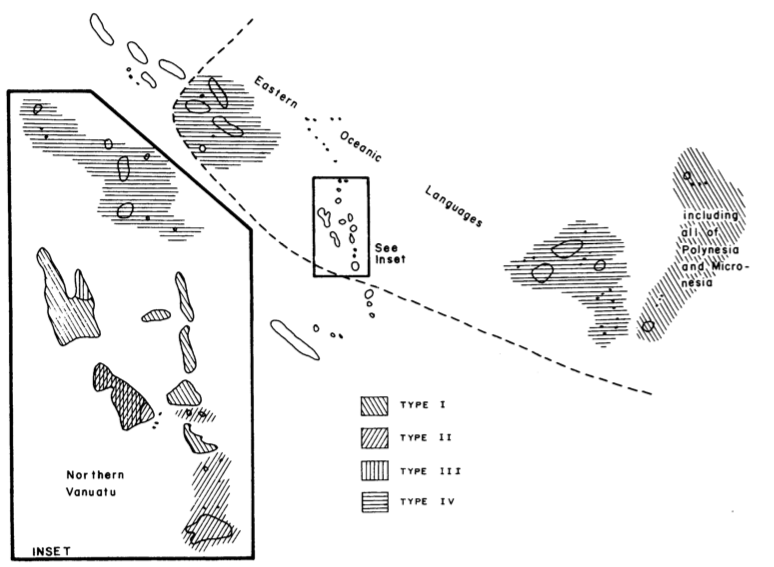
\includegraphics[width=8cm]{illustrations/crowley_1985_map.png}
%\caption[Map of four different types of common noun phrase markers in Oceanic from Crowley(1985).]{\textbf{Map of four different types of common noun phrase markers in Oceanic from \citet[162]{crowley1985common}. Type 1: absence of common noun phrase marker or marker is not a reflex of \emph{*na /*a}, type 2: non-productive system involving a reflex of \emph{*na /*a}, type 3: productive marking involving \emph{*na /*a} as a prefix that is regularly separable from the noun and type 4: productive marking involving \emph{*na /*a} generally existing as a free-standing marker.}}
%\label{fig:crowley_map}
%\end{figure}

%In contrast, the corresponding feature in Grambank is `GB022: \emph{Are there prenominal articles?'} (see Fig.~\ref{fig:gb022_map}). Languages that have \emph{te} (like M\={a}ori) or reflexes of \emph{*na/*a} as articles before the noun both count as ``yes'' (1) for GB022 and those that have no prenominal marker as a ``no'' (0). This Grambank feature splits Crowley's type 1 into two categories, and combines all the languages with reflexes of \emph{*na/*a} and \emph{te} (or other markers) into one category. We can now distinguish those that have a prenominal article from those that do not, but we cannot tell apart those which have retained the proto-form from those which have not. Since many reconstructions of grammar in historical linguistics rely on particular forms, this is an important difference. This does not matter for features such as word order.

%\begin{figure}
%\centering
%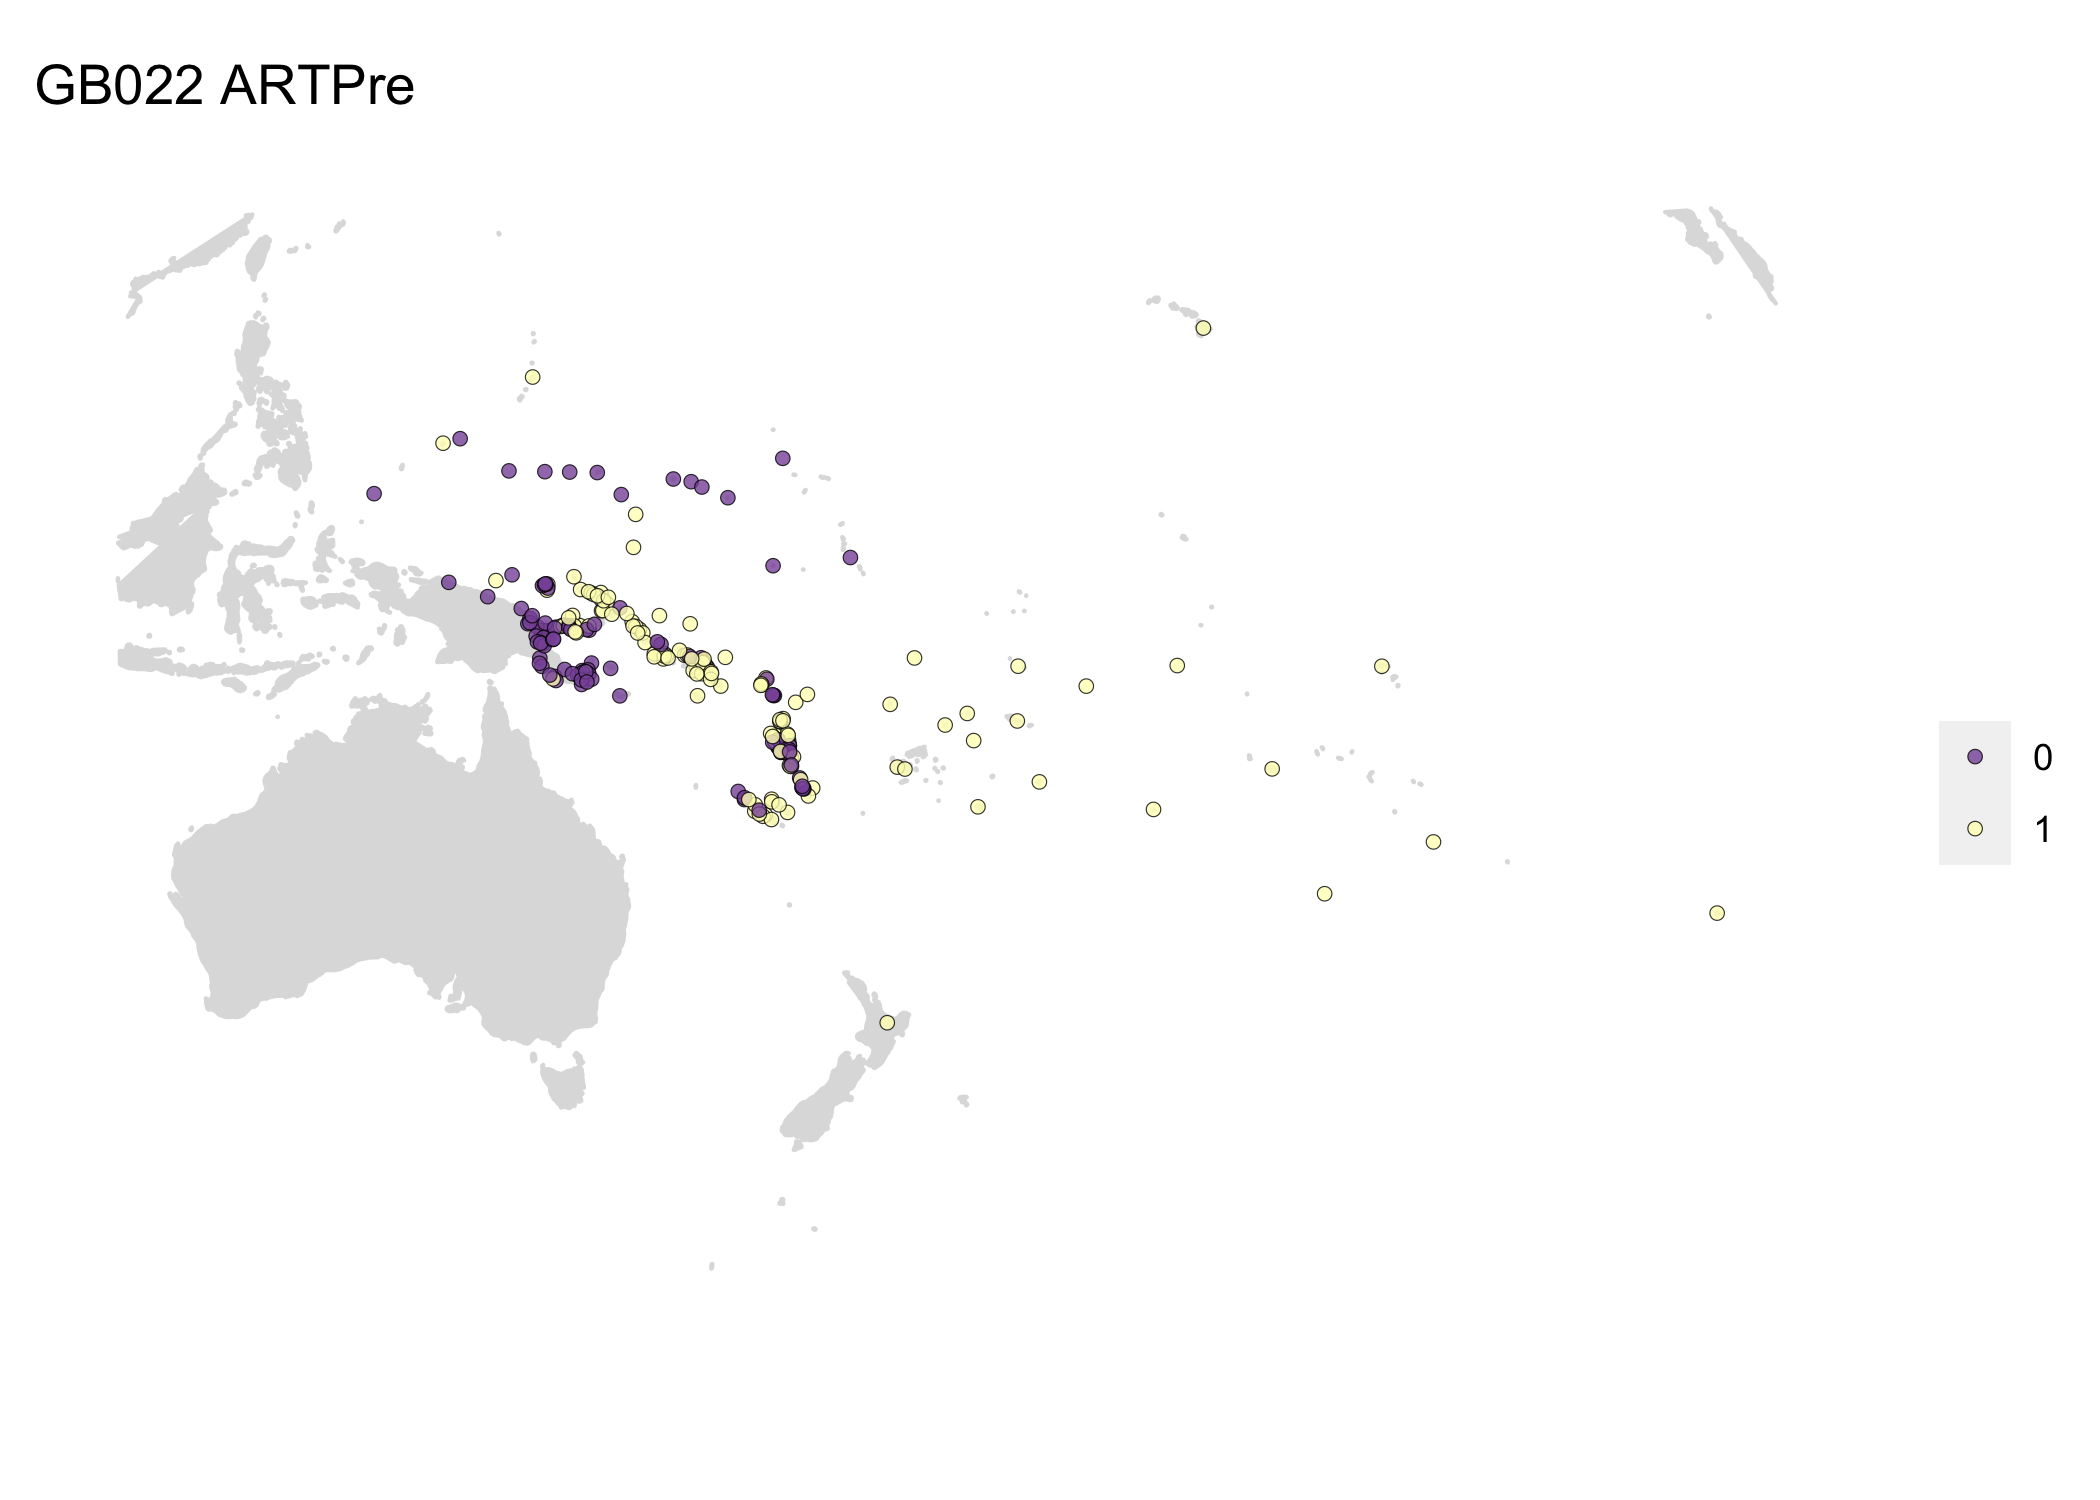
\includegraphics[width=16cm]{illustrations/plots_from_R/coverage_plots/maps/map_GB022.png}
%\caption{{Map of Austronesian languages for GB022 \emph{Are there prenominal articles?} Yellow = ``yes", purple = ``no".}}
%\label{fig:gb022_map}
%\end{figure}

%The data in this study is composed of abstract features such as ``is a grammatical distinction made between X and Y?''. This makes it different from most studies of grammatical features in historical linguistics. As was noted earlier, it is possible for two languages to be coded alike but not share ancestry. It is also possible that such abstract features track something beyond the particular forms. \citet[503]{ross2004morphosyntactic} notes that a particular structure of the pronominal system of Mokilese is maintained, despite the formal markers being continuously replaced. He argues that there are discourse related reasons for maintaining this system and that the interaction between this construction and the rest of the grammar is such that the distinction is maintained. When particular markers are lost in this system, new ones appear in their place\footnote{He also notes that Goddard has observed similar patterns in Algonquian languages \citep{goddard1993algonquian}.}. This may be true of more features, and in such cases languages can share a grammatical feature but not have the same particular expression, and this could be due to inheritance. In addition, in many instances --- particularly within families --- abstract features such as 'GB022: \emph{Are there prenominal articles?}' are in fact correlated with specific forms even if the forms are not explicitly being tracked.

%Furthermore, it is possible that due to the interconnectedness of structural features related languages can develop similarily without 
%Related languages may also show similarity due to inheritance, even if the relevant state was not present in the ancestor, as the quote from \citet{chung1977aspects} earlier continues:

%\begin{quotation}
%\noindent\emph{[I]t is also reasonable that changes begun in a Proto-language may have continued even after its separation into daughter languages. In this way, related languages may come to share a feature which existed only in embryonic form, or not at all, in their common ancestor}\footnote{This idea is important to a particular hypothesis about Proto-Polynesian syntax, because according to \citet{chung1978} Proto-Polynesian was accusative and Tongan and S\={a}moan both developed ergativity semi-independently while the Eastern Polynesian languages (which are more closely related to S\={a}moan than to Tongan) did not develop this feature.}.
%\end{quotation}
%\begin{flushright} \citet[539]{chung1977aspects} \end{flushright}
%
%This theory proposes that the conditions for developing a certain feature may have been present in the ancestral language even if the feature itself is absent. It is therefore likely that the daughter languages would develop it even if they were isolated from each other, because they have inherited the prerequisites for developing the feature. This is similar to what is known in the literature on cultural evolution as ``preadaptation'' \citep{scott2010language}. One might say that the seed is sown already in the parent language, and that as a result its daughter languages will likely turn out a certain way.
%
%This ties in with the dependencies of features, insofar as dependencies are representations of features ``moving as a group'' through time. If some of these features are reliable ``early movers'', one could use them to predict certain developments in daughter languages. This theory aligns well with a view of language as a system where everything neatly fits (``La langue est \emph{un système où tout se tient}'' [language is systematic / a system where everything fits], Saussure \citep{koerner1997notes}). This is in contrast to the view by, among others, \citet[328]{bloomfield1933language} who stated that \emph{every word has its own history}. It is likely that systematic effects like these are more probable in structural data than in lexical data.
%
%However, in this analysis we are investigating each feature separately so it is not possible to derive information about features co-evolving. It is also difficult for the algorithm \emph{not} to reconstruct a certain state in the parent language, if the majority of daughter languages possess it. This is one instance where knowledge of plausible paths and profiles of languages from classical linguistics may contribute information that is, so far, not possible to retrieve using computational means.

%In summary, the comparative method of historical linguistics involves Maximum Parsimony coupled with information on plausibility. It is not possible in computational reconstruction to take plausibility into account since it has not been formalised. The kind of data typically used in reconstruction of grammar in historical linguistics concerns specific forms, whereas the data for this paper is structural features.

\subsection{Computational phylogenetic methods}
\label{sec:asr_methods}
%This section outlines the computational methods of ASR which will be used in this study, and contrasted with the conventional approaches in historical lingusitics outlined in section \ref{sec:ars:metod:hist}.
In recent years, linguists have begun to apply computational phylogenetic methods from biology to the reconstruction of linguistic history. Biologists have, similarly to linguists, been interested in inferring trees of the genetic relationship between species\footnote{Interestingly, the use of trees in linguistics and biology first occurred in publications just one year apart with \citet{schlegel1808sprache} publishing a tree of languages and \citet{lamarck1809philosophie} a tree of species. However, as \citet[370]{greenhill2015evolution} notes, it was not until Darwin's publication of \emph{The Origin of Species} in  \citeyear{darwin1859origin} that the concept of species trees in biology truly took off.}, ancestral states and the tempo and mode of evolution \citep{atkinson2005curious}. Biologists and linguists may have inspired each other, but methodologically the fields progressed separately for a long time \citep[370]{greenhill2015evolution}. Both fields are interested in answering similar questions: how are these languages/species related?, what was the earlier state of a language/species?, which traits are changing slower/faster? etc. The two fields have developed different methodologies, with biologists leaning more towards quantitative computational methods for tree construction and ASR compared to linguists who have focused more on rigorous tests for which linguistic data is valid for analysis (see for example the Double Cognacy Criteria in \citet{walkden_2013}). It is possible that this is due to the material under study, it may be more difficult to tease our non-trivial similarities in languages than in species (especially since genome sequencing became more readily available).

% \section{Computational methods}

Applying computational methods of ASR to linguistic data is becoming more common. \citet{jager2018using} apply three different methods (Maximum Parsimony, Maximum Likelihood and Minimal Lateral Networks) to cognate class reconstruction in three different language families. The aim of that study was primarily to evaluate how often the methods reconstructed the same state as what the authors label ``the Gold Standard'' (reconstructions by traditional historical linguists using the classical Comparative Method). This is similar to the study at hand; one of the aims of this paper is to estimate the degree of concurrence between computational methods using typological database data and conventional approaches in historical linguistics. The data that serves as input to the computational machinery in \citet{jager2018using} was annotated by ``hand'' for cognacy by historical linguists, meaning that the identification of cognate classes is still an entirely human affair (task one in Fig. \ref{fig:HL_tasks}). This is also true for this study, the identification of structural features in languages is a human process. The overall result of \citet{jager2018using} was that Maximum Likelihood performed the most similar to traditional historical linguistics ASR, but that there were still several shortcomings. Most notable of these were undetected borrowings, variation within languages and parallel independent shifts. In this paper, we address the potential for contact events by using sets of trees from a Bayesian posterior (as \citet{jager2018using} also do), some of which may represent an alternative contact history (see section \ref{the_trees}). 

There are also two recent studies of Indo-European grammatical history: \citet{carling2021reconstructing} and \citet{goldstein_2022}. \citet{carling2021reconstructing} evaluate different theories of the history of the morphosyntax of Indo-European by comparing these to the product of computational Bayesian phylogenetic modelling. They find support for the ``canonical'' model of Indo-European syntax. Goldstein in his paper challenges a commonly applied principle in the reconstruction of Indo-European syntax; the ``frequency heuristic'' which holds that \emph{if the number of homologous elements (e.g., lexical cognates) in the daughter languages meets a minimum threshold (canonically three), their ancestor is reconstructed to the root of the tree} \citep[1/71]{goldstein_2022}. This is done because scholars argue that the true tree is unknown and that this is an appropriate method in the absence of the true tree. Goldstein argues that the appropriate action is instead to carry out reconstruction on many different trees that represent possible histories --- a Bayesian posterior tree sample. He argues that this is methodologically more sound and because the results of his approach are in accord with the consensus in historical linguistics it strengthens their validity.

Both \citet{carling2021reconstructing} and \citet{goldstein_2022} use a Bayesian method of ASR within the Continuous-Time Markov Chain (CTMC)-framework\footnote{The main difference between the methods of \citet{carling2021reconstructing} and \citet{goldstein_2022} is that \citet{carling2021reconstructing} use a tree structure informed by \citet{chang2015ancestry} and comparative-historical \emph{communis opinio} and vary the branch lengths 10,000 times in a principled and informed manner to generate 10,000 different trees while \citet{goldstein_2022} takes 100 random samples directly from the posterior of \citet{chang2015ancestry}.}. This approach comes with certain important assumptions, to quote from \citet[77]{goldstein_2022}:

\begin{quotation} \emph{
CTMCs model language change as a stochastic phenomenon with rate parameters that govern the amount of time between transition events. It is worth highlighting the assumptions that these models bring with them. First, character states at the nodes of a tree are assumed to depend only on the state of their immediate ancestors and the length of the branch along which they evolved (Cathcart 2018:4). Second, the probability of a transition depends only on the current state of a language. Its previous history is irrelevant. This is known as the markov property. Finally, rates of gain and loss are assumed not to vary across the tree.}
\end{quotation}

It is always important to be up-front and explicit about the assumptions an approach takes and evaluate if they make sense for the given situation. For linguistic data, these assumptions do seem to hold. For more details on the methods, please see  \citet{goldstein_2022}, \citet{pagel2004bayesian}, \citet{ronquist2004bayesian} and \citet{liggett2010continuous}. 

Another popular method of ancestral state reconstruction is Stochastic Character Mapping (SCM, \citet{huelsenbeck2003stochastic}). SCM is a procedure that simulates character histories using Continuous Time Markov-rates. These rates are usually estimated on the basis of the tree topology and the data attested at tree tips before SCM is carried out, but can also be defined in other ways. SCM can follow the same CTMC approach employed by \citet{carling2021reconstructing} and \citet{goldstein_2022}, but not necessarily\footnote{Thank you to one of the anonymous reviewers of Diachronica for highlighting this.}.

%reviewer 2: This statement is imprecise. SCM is a procedure that simulates character histories using CTM rates. These rates are usually estimated on the basis of the tree topology and the data attested at tree tips before SCM is carried out. So SCM is a procedure that can follow the method described by Goldstein (but can also be used with arbitrarily defined rates).

Computational approaches to reconstruction not only allow us to effectivize the process by inferring the prior states of hundreds of traits in a short span of time, but they also allow us to apply exactly the same principles in exactly the same way to all pieces of data. This is much harder to do manually, since different scholars may use slightly different assumptions and judgement when conducting ASR. One could say that what we lose in deep human insight, we gain in consistency and speed. Furthermore, if the deep human insight of historical linguistics could be quantified into priors that can be fed into computational models --- we may not need to lose anything. Unfortunately, this is not the case currently, but it may be possible in the future.
%Any assumptions about plausibility of changes or states needs to be explicitly included into the model, and applied identically across the sample.


\FloatBarrier
\section{Material and methods}
\subsection{Methods: Maximum Parsimony, Maximum Likelihood and Most Common}
\label{sec:MP_ML_MC}
In this study, we will be reconstructing the presence or absence of structural features in proto-languages of the Oceanic subgroup using Maximum Parsimony, Maximum Likelihood and Most Common. This section gives a brief overview of the three methods. Further technical details concerning the precise application can be found in the supplementary material \ref{supp:tech_details}. For an extensive comparison of different methods of ancestral state reconstruction and their advantages, see \citet{joy2016ancestral}.

\textbf{Maximum Parsimony} finds the set of ancestral states that result in the fewest number of changes between nodes (also known as ``lowest Parsimony cost''). If we think of the rate of change as the number of changes in the tree, then Maximum Parsimony selects the candidate solution with the slowest rate out of all possible solutions it can choose from. Maximum Parsimony is intuitively simple. While the principle of ``Maximum Parsimony'' is practised in traditional ASR in historical linguistics, it should be noted that they rarely use the term \emph{per se}, but rather the description of ``fewest number of changes along the tree''.

Maximum Parsimony may be simple and intuitive, but it is not without its critics. Part of the critique is that it does not take into account branch lengths in the tree (the time between splitting events). Furthermore, Maximum Parsimony necessarily assumes that the solution that posits the fewest changes (slowest possible rate of change) is also the most probable one. This is not necessarily a valid assumption; some features may evolve at a faster rate than Maximum Parsimony predicts. Both of these disadvantages are addressed in the second method we will be applying: Maximum Likelihood.

%The second method which will be applied in this study is that of \textbf{Maximum Likelihood}. 
%\subsection{Maximum Likelihood}
Ancestral state reconstruction using \textbf{Maximum Likelihood} posits the most likely ancestral state distributions based on the overall probabilities given all the nodes in the tree and all branches. This approach does not assume that the slowest rate of change is the most probable one. If, for example, the distribution of values at the tips is very scattered, with sibling pairs frequently having different values, Maximum Likelihood will infer that the feature has a high rate of change and use that information when positing ancestral states as well. The Maximum Likelihood algorithm assigns probabilities of state changes and distributions based on branch lengths. A mutation along a shorter branch is given more weight in the likelihood calculations than if it occurred in a longer branch. Furthermore, reconstruction using Maximum Likelihood allows us to use a model of change where we do not assume that the rates for losses (1$\rightarrow$0) are equal to the rate of gains (0$\rightarrow$1). In this study, we use an ``All Rates are Different" (ARD) model, which allows for the rate of loss and gain to be different\footnote{Similarly to the studies by \citet{carling2021reconstructing} and \citet{goldstein_2022}, rates cannot vary within the tree in this study.}. It is possible to further specify the model, for example by specifying transition rates, specify certain nodes beforehand etc. For this study, this was not done since there is no information to base these decisions on. Specifically, we are also using a marginal Maximum Likelihood estimation, for more details see supplementary material \ref{supp:tech_details}.

While Maximum Parsimony and conventional HL-ASR are similar, they have differences as well. It is impossible for Maximum Parsimony to take into account branch lengths, nor can it assume anything but the slowest rate of change or posit different rates for losses and gains. It is, however, possible that historical linguists estimate something similar when they take into account the ``plausibility of the changes posited''. It is possible that scholars of historical linguistics take the length of time into account or assume that a loss is more likely than a gain for a given feature. In this study, we compare Maximum Parsimony and Maximum Likelihood reconstructions to the conventional ASR in historical linguistics. If the results from conventional historical linguistics are more similar to that of Maximum Likelihood, a potential explanation would be that the ``plausibility of changes posited'' is indeed operating along similar lines as Maximum Likelihood by taking branch length into account and assuming varying rates of change.

%\subsection{Methods: Most Common}
We will also compare the predictions of historical linguists with a ``dummy-model'' which is based solely on which value is the \textbf{Most Common} in the daughter languages of a given proto-language --- entirely disregarding the tree structure\footnote{This is similar to the frequency heuristic described in \citet{goldstein_2022}.}. In the toy example in Fig. \ref{fig:clark_tree}, this approach would reconstruct that the root had feature value ``X''. Whether we prefer Maximum Parsimony, Maximum Likelihood or another approach to reconstruction, it should be the case that actually taking the tree structure into account is the sounder methodology. %We expect that both methods has a higher degree of concordance with the findings in historical linguistics compared to only counting which value is most common.

All analysis have been calculated in \texttt{R} \citep{R} using the packages \texttt{castor} (Parsimony, \citet{louca2017efficient}), \texttt{phangorn} (Parsimony, \citet{phangorn}) and \texttt{corHMM} (Maximum Likelihood, \citet{R-corHMM}). The packages \texttt{ape} \citep{paradis2004ape}, \texttt{adephylo} \citep{jombart2017package}, phytools \citep{revell2012phytools}, psych \citep{psych_r_package},  reshape2 \citep{wickham2020reshape2} and tidyverse \citep{tidyverse13} were also used for data wrangling, analysis, summarising and visualising\footnote{For a complete record of all R-packages used, see the supplementary material \ref{supp:r_packages}.}.

All of the R-code and data necessary for the analysis in this paper will be published alongside the paper, in Supplementary Materials and in archived web-storage (Zenodo).

\textcolor{red}{Stand-in URL until zenodo-release (in case editing staff want a change in plots etc):}
\url{https://github.com/HedvigS/Oceanic_computational_ASR}

%The third method employed is \textbf{Stochastic Character mapping}. This method was proposed by \citet{huelsenbeck2003stochastic} and is an extension of an approach suggested by \citet{nielsen2002mapping}. 
 \FloatBarrier
\subsection{Calculation of similarity between predictions from conventional HL and computational approaches}
\label{result_calc_section}
We calculate the similarity of the predictions of historical linguists and computational methods with a measure of concordance\footnote{This metric is also known as \textit{accuracy} in machine learning, but we do not use that term because we wish to avoid the connotation that what is being measured is the real-world accuracy of the reconstruction as opposed to the agreement between methods.}. Concordance measures how closely the computational reconstruction matches historical linguists' reconstruction --- how much they concur. It is measured as the number of agreements about grammatical features (i.e. Grambank binary questions) of predicted proto-languages, divided by the total number of grammatical features predicted. 

%In addition to these two scores we will also calculate how much better each method does compared to just counting which is the most common vale of a feature in the daughter languages. As we learned in section \ref{sec:ars:metod:hist}, simply relying on frequency and not taking the tree structure into account can lead us astray. Whether we prefer Maximum Parsimony, Maximum Likelihood or another approach to reconstruction it should be the case that actually taking the tree structure into account is the more sound methodology. We expect that both methods has a higher degree of concordance with the findings in historical linguistics compared to only counting which value is most common.

For each feature, the methods predict a distribution of the two states (presence and absence) for every ancestral node. If the distribution is majority presence (more than 60\% of the ancestral state is ``1'') it is registered in the results as ``Presence''; if less than 40\% presence it is registered as ``Absence''. If the ancestral state is between 40-60\% of either state, the prediction is registered as ``Half/Half''. This was done to highlight the amount of uncertainty the results sometimes contain, while at the same time making it a fair comparison between Maximum Parsimony and Maximum Likelihood. Comparing the raw distributions themselves is not a fair comparison because Maximum Parsimony is always more likely to suggest 0, 0.5 or 1 results (because the majority of the splits in the tree are binary) whereas Maximum Likelihood rarely produces exactly 0 or 1. Rounding into these bins also makes it possible to derive the number of ``True Negatives'', ``True Positives'' etc which allows for the calculation of concurrence scores.

If the reconstruction of a feature by HL experts for an ancestral node was ``Presence'' and the algorithm did predict presence with over 60\%, it is counted as a ``True Positive'', and so on\footnote{The terms ``True'' and ``False'' are used here in accordance with terminology in machine learning. In this instance, they are indicating whether the results from the computational method and historical linguists agree (True) or not (False). It should not be interpreted as a measure of empirical ``Truth'' necessarily.}. Table~\ref{example_HL_prediction_table_true_positives} illustrates how the results are summarised.

\begin{table}[ht]
\centering
\caption{Table illustrating how the results of ancestral node predictions are calculated.}
\label{example_HL_prediction_table_true_positives}
\begin{tabular}{|p{4cm}|p{6cm}|p{6cm}|l|l|l|l|l|}
\hline
\textbf{Finding in historical linguistics} & \textbf{Prediction by Computational Method} & \textbf{Result} \\ \hline
Absence & >60\% Absence & True Negative \\ \hline
Absence & >60\% Presence & False Positive (type 1-error) \\ \hline
Presence & >60\% Presence & True Positive \\ \hline
Presence & >60\% Absence & False Negative (type 2-error) \\ \hline
Absence & 40-60\% Presence/Absence & Half \\ \hline
Presence & 40-60\% Presence/Absence & Half\\ \hline
\end{tabular}
\end{table}

For each method, a plain concordance score (Eq \eqref{eq:accuracy}) is then calculated. The score is calculated between all computational methods and the conventional historical linguists' prediction and also between all computational methods themselves \footnote{When comparing one computational method result to another, ``half'' - ``half'' count as a True pair. Otherwise the scoring is the same.}.

\begin{equation}\label{eq:accuracy}
\frac{\text{True Negative + True Positive}}{\text{True Negative + True Positive + False Negative + False Positive}}
\end{equation}

It is also important to take into account the Half-results. This count represents instances where the method was not able to say with strong confidence that something was present or absent. The reason it is interesting to separate these out is that while they may indicate a majority result in one direction, it is not far from suggesting the direct opposite. For example, if one of the methods reconstructs Proto-Oceanic as having a 51\% chance of having ergative marking --- it is not far away from suggesting that this marking is absent. In order to take these types of cases into account the cut-off of 40\%-60\% was set and summarised as "Half" results. We can apply the concordance score to this summary statistic as well, as shown in Eq. \eqref{eq:accuracy_incl_half}. 

\begin{equation}\label{eq:accuracy_incl_half}
\frac{\text{True Negative + True Positive} + \frac{\text{Half}}{2}}{\text{True Negative + True Positive + False Negative + False Positive + Half}}
\end{equation}

Both scores will be reported, but we will rely mainly on the concordance score with the inclusion of the Half-results. This is because this approach takes into account the possible uncertainty of the half-scores which can be valuable information.

In a similar study of ancestral states of cognate classes, \citet{jager2018using} compared three different methods of ancestral state reconstruction for lexical data (cognate classes): Maximum Parsimony, Maximum Likelihood and Minimal Lateral Networks. They found that reconstructions using Maximum Likelihood performed the most like the predictions by historical linguists. However, \citet{jager2018using} describe the general performance of all the computational reconstruction methods they used as ``poor''. \citet{jager2018using} evaluated the methods using F1-scores which is the harmonic mean of Precision and Recall \citep{sasaki2007truth}. This way of evaluating performance focused on True Positives and ignores True Negatives altogether. It was suitable for the study by \citet{jager2018using} because they were primarily interested in the presence of cognate classes, which makes disregarding True Negatives admissible. This is not the case here, True Negatives for structural features are meaningful in a different way than the absence of cognate classes. Because of this, we will not report F1-scores in the main text but only in the supplementary material (see Supplementary Material \ref{f1_results} and \ref{math_supp} \footnote{I am very grateful for mathematical assistance from Stephen Mann in regards to the F1-score including half results calculation.}). %The highest (``best'') F1-score in \citet{jager2018using} was 0.79 (Austronesian language sample, Maximum Likelihood), and the worst was 0.44 (Indo-European, Minimal Lateral Networks).

% mutate(F1_score = 2 * ((Precision*Recall)/(Precision + Recall)), 
  %         F1_score_incl_half = 2 * ((Precision_incl_half *Recall_incl_half)/(Precision_incl_half + %Recall_incl_half)) )%>% 
 
In addition, we also tested the strength of correlations between agreement with HL and measurements of phylogenetic signal on one hand and the distribution of tips in each state on the other. For this comparison, we are comparing each method separately against the HL-agreement and phylogenetic signal/distribution of states. For this reason, we did not use the above approach of binning results into Presence, Half or Absence but used the predicted values from the method directly instead (see Supplementary Materials \ref{supp:cor_d_HL} and \ref{supp:cor_min_p_HL}.

%In order to evaluate the results, we need to calculate a concordance score per method and tree. \citet{jager2018using} use the F1-score (harmonic mean between precision and recall) in their study of how computationally reconstructed lexical proto-forms compare to those reconstructed by historical linguists. For example, if for a given proto-language there are 60 features reconstructed by experts and the algorithm result is 10 True Positives, 10 False Positives, 10 True Negatives, 10 False Negatives and 20 ``Half/Half'' then the F1-score is 0.5 (recall = 10 / (10+10) = 0.5, precision = 10 / (10+10) = 0.5 and F1-score = 2 *((0.5*0.5) / (0.5 + 0.5) = 0.5)). Note that the F1-score disregards True Negatives and Half /Half-results.

%F1-scores will be reported because they are insightful and have been used in similar studies. However, the F1-formula ignores the amount of True Negatives and Half/Half results. Therefore, in addition we will also calculate a simpler concordance score; how many concordant predictions did the algorithm make given all the predictions it made (aka ``accuracy'')? For example, if for a given proto-language there are 60 features predicted by experts with the same distribution of results as in the example above, then the concordance score would be (10 + 10)/40 = 0.5. We can also include the Half/Half-predictions, awarding 0.5 points for at least not strongly predicting a false value. In that case, this example has a concordance score of 0.5 ((10 + 10 + (20/2)) / 60). These scores all reflect different ways of assessing concordance and will give different perspectives on our results and how our algorithms are performing. %Features where there were more than half of the data-points missing in the tree were not to be included. hankfully there were no occurrences of this.

%\begin{equation} \label{accuracy_incl_half}
%\frac{\text{agree} + \frac{\text{half}}{2}}{\text{all reconstructions}}
%\end{equation}
\FloatBarrier
\subsection{Data}

\subsubsection{The Grambank-dataset}
\label{asr:sec:GBcoverage}

The data for the study is taken from the Grambank-project \citep{grambank_release}. The Grambank dataset consists of 195 structural features which have been coded by a large group of research assistants for over 2,400 languages. This dataset includes 280 Oceanic languages. 

%The Grambank project is part of the Glottobank consortium, which is a collaboration between the Max Planck Institute for the Science of Human History in Jena (MPI-SHH), the Australian National University, the Australian Research Council's Centre of Excellence for the Dynamics of Language and the University of Auckland. The project is led by a team of senior linguists (Russell Gray, Simon Greenhill and Quentin Atkinson) and employs student assistants as coders in Kiel, London, Canberra, Uppsala and a few other locations. Coders who have been contributed significantly to the database are included as co-authors of the upcoming release paper \citep{grambank_release}, alongside other contributors. I have personally participated in this project as a coder and as a coordinator.

%The aim of Grambank is to provide a consistently coded set of structural features of the world's languages for research questions relating to history, complexity and more. The dataset will be published openly. 
 
%The Grambank dataset builds on previous typological work by \citet{dunnetal2005, dunn2008, reesinketal2009, dunnreesink2012} and \citet{ntswebsite}. The project has a global focus and the aim is to include all languages in the world that are described for their core grammatical structure. 

% In the work by Dunn, Reesink and colleagues, they were particularly focussed on languages of Oceania and Australia and the prehistory of migrations and contact there. The Nijmegen Typological Survey-project \citep{nts2014, ntswebsite} on the other hand was focussed on African languages.

The questionnaire's 195 questions cover what are often called the ``core domains'' of traditional grammatical description: word order, possession, negation, tense, aspect, mood, deixis, interrogation, comparatives and more. Features are included in the questionnaire if it is likely that it is possible to code them for the majority of the world's languages which have been described grammatically (approx 4,000 languages, see \citet{hammarstrom2018simultaneous}). This means that rarer features are not included such as family or region-specific ones. The full questionnaire is found in appendix \ref{Grambank_features}.

The Grambank dataset is coded by student, research assistants and other collaborators under the supervision of expert linguists. Each feature is accompanied by documentation guiding coders so that the questionnaire is applied as consistently as possible across different languages. For more details on the coding workflow of Grambank, see \citet{slingerland2020coding}. %For further details on the dataset, see Supplementary Material ~\ref{supp:dataset_details}.

There are differences between how grammatical structures are described in the historical linguistics literature and how they are defined in Grambank, for more on this see section \ref{sec:POC_lit_review}.

%It is crucial in a cross-linguistic survey of this kind that the features are applied consistently across all languages of the sample. Within the Grambank-project, we strive towards a high level of consistency between coders. There are many coders employed and we have established work-flows to ensure that the features are applied consistently across languages. New coders are trained in the workflow and linguistic definitions through collaborative coding. Each feature in the questionnaire is accompanied by a helpful and pragmatic definition in a wiki-page. Each feature is also associated with a ``patron'', an expert linguist assigned to a set of features who has the final word should any further clarification be needed or disagreements arise. There are seven patrons in the project: Alena Witzlack-Makarevich, Harald Hammarström, Hannah Haynie, Jeremy Collins, Jay Latarche, Jakob Lesage and myself. All coders in the project are able to converse with each other and patrons through GitHub, an online platform for project coordination and code collaboration. When we are unable to make a coding decision with sufficient confidence, the data-point is marked as ``?''.

\FloatBarrier
\subsubsection{Data coverage} 
This study is focused on the Oceanic subgroup of the Austronesian language family. The Oceanic subgroup covers almost all languages in Remote Oceania (with the exceptions of Chamorro and Palauan) and large parts of Near Oceania. Fig.~\ref{Oceanic_map} from \citet[2]{protooceanicvol5} shows the extent of the major subgroups of the Austronesian language family, with Oceanic covering the largest surface area. Following the language classification of Glottolog 4.5 \citep{glottolog4_5}, there are 522 languages in total in the Oceanic subgroup.

\begin{figure}[ht]
\centering
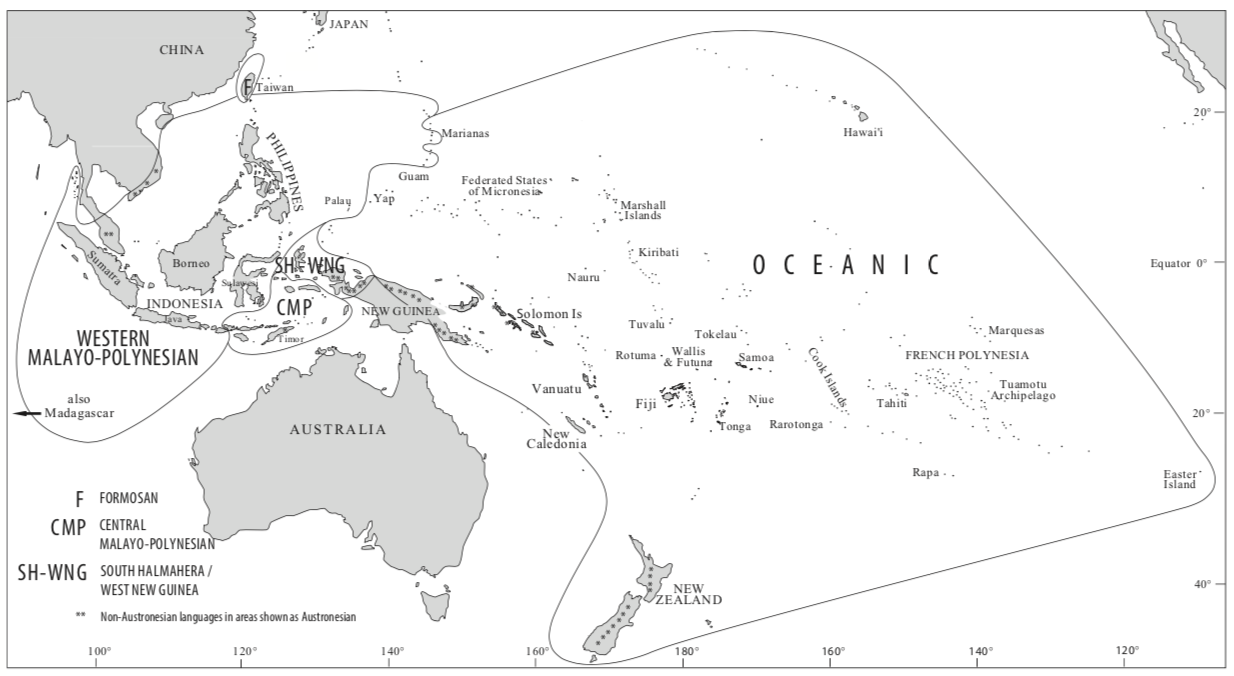
\includegraphics[width=17cm]{illustrations/ross_pawley_osmond_protooceanic_vol5.png}
\caption{{Map of the Austronesian language family and major subgroups, from \citet[2]{protooceanicvol5}.}}
\label{Oceanic_map}
\end{figure} 

Not all languages of the Oceanic subgroup have a grammatical description, but out of those that have it, nearly all are included in Grambank. Table~\ref{GB_coverage_table_island_group} shows the coverage of Oceanic languages in the entire dataset. According to Glottolog, there are 289 Oceanic languages that have a grammar or a grammar sketch. Out of these 180 are included in grambank. The map in Fig.~\ref{GB_austro_coverage} shows the same coverage information, with languages coded for their data coverage status.

% latex table generated in R 4.2.0 by xtable 1.8-4 package
% Wed Jun 22 18:04:34 2022
\begin{table}[ht]
\centering
\begin{tabular}{p{5cm}p{2.7cm}p{2.7cm}p{2.7cm}p{2.7cm}}
  \hline
Island group & grammar doesn't exist & grammar exists (not in GB, yet) & Less than half of features covered in GB & More than half of features covered in GB \\ 
  \hline
Bismarck & 5 & 1 & 7 & 42 \\ 
  Central Pacific & 11 & 0 & 1 & 33 \\ 
  Central Vanuatu & 42 & 0 & 1 & 48 \\ 
  Interior New Guinea & 11 & 0 & 0 & 4 \\ 
  Micronesia & 6 & 0 & 1 & 16 \\ 
  N Coast New Guinea & 77 & 2 & 3 & 19 \\ 
  New Caledonia & 18 & 1 & 0 & 14 \\ 
  Northern Vanuatu & 9 & 0 & 0 & 5 \\ 
  S New Guinea & 36 & 3 & 1 & 26 \\ 
  Solomons and Bougainville & 25 & 1 & 4 & 30 \\ 
  Southern Vanuatu & 1 & 0 & 0 & 8 \\ 
  Temotu & 3 & 0 & 2 & 5 \\ 
  Total & 244 & 8 & 20 & 250 \\ 
   \hline
\end{tabular}
\caption{Table showing coverage of Oceanic languages in Grambank per island group with matches to the Gray et al 2009-tree} 
\label{GB_coverage_table_island_group_gray}
\end{table}


\begin{sidewaysfigure}[ht]
\centering
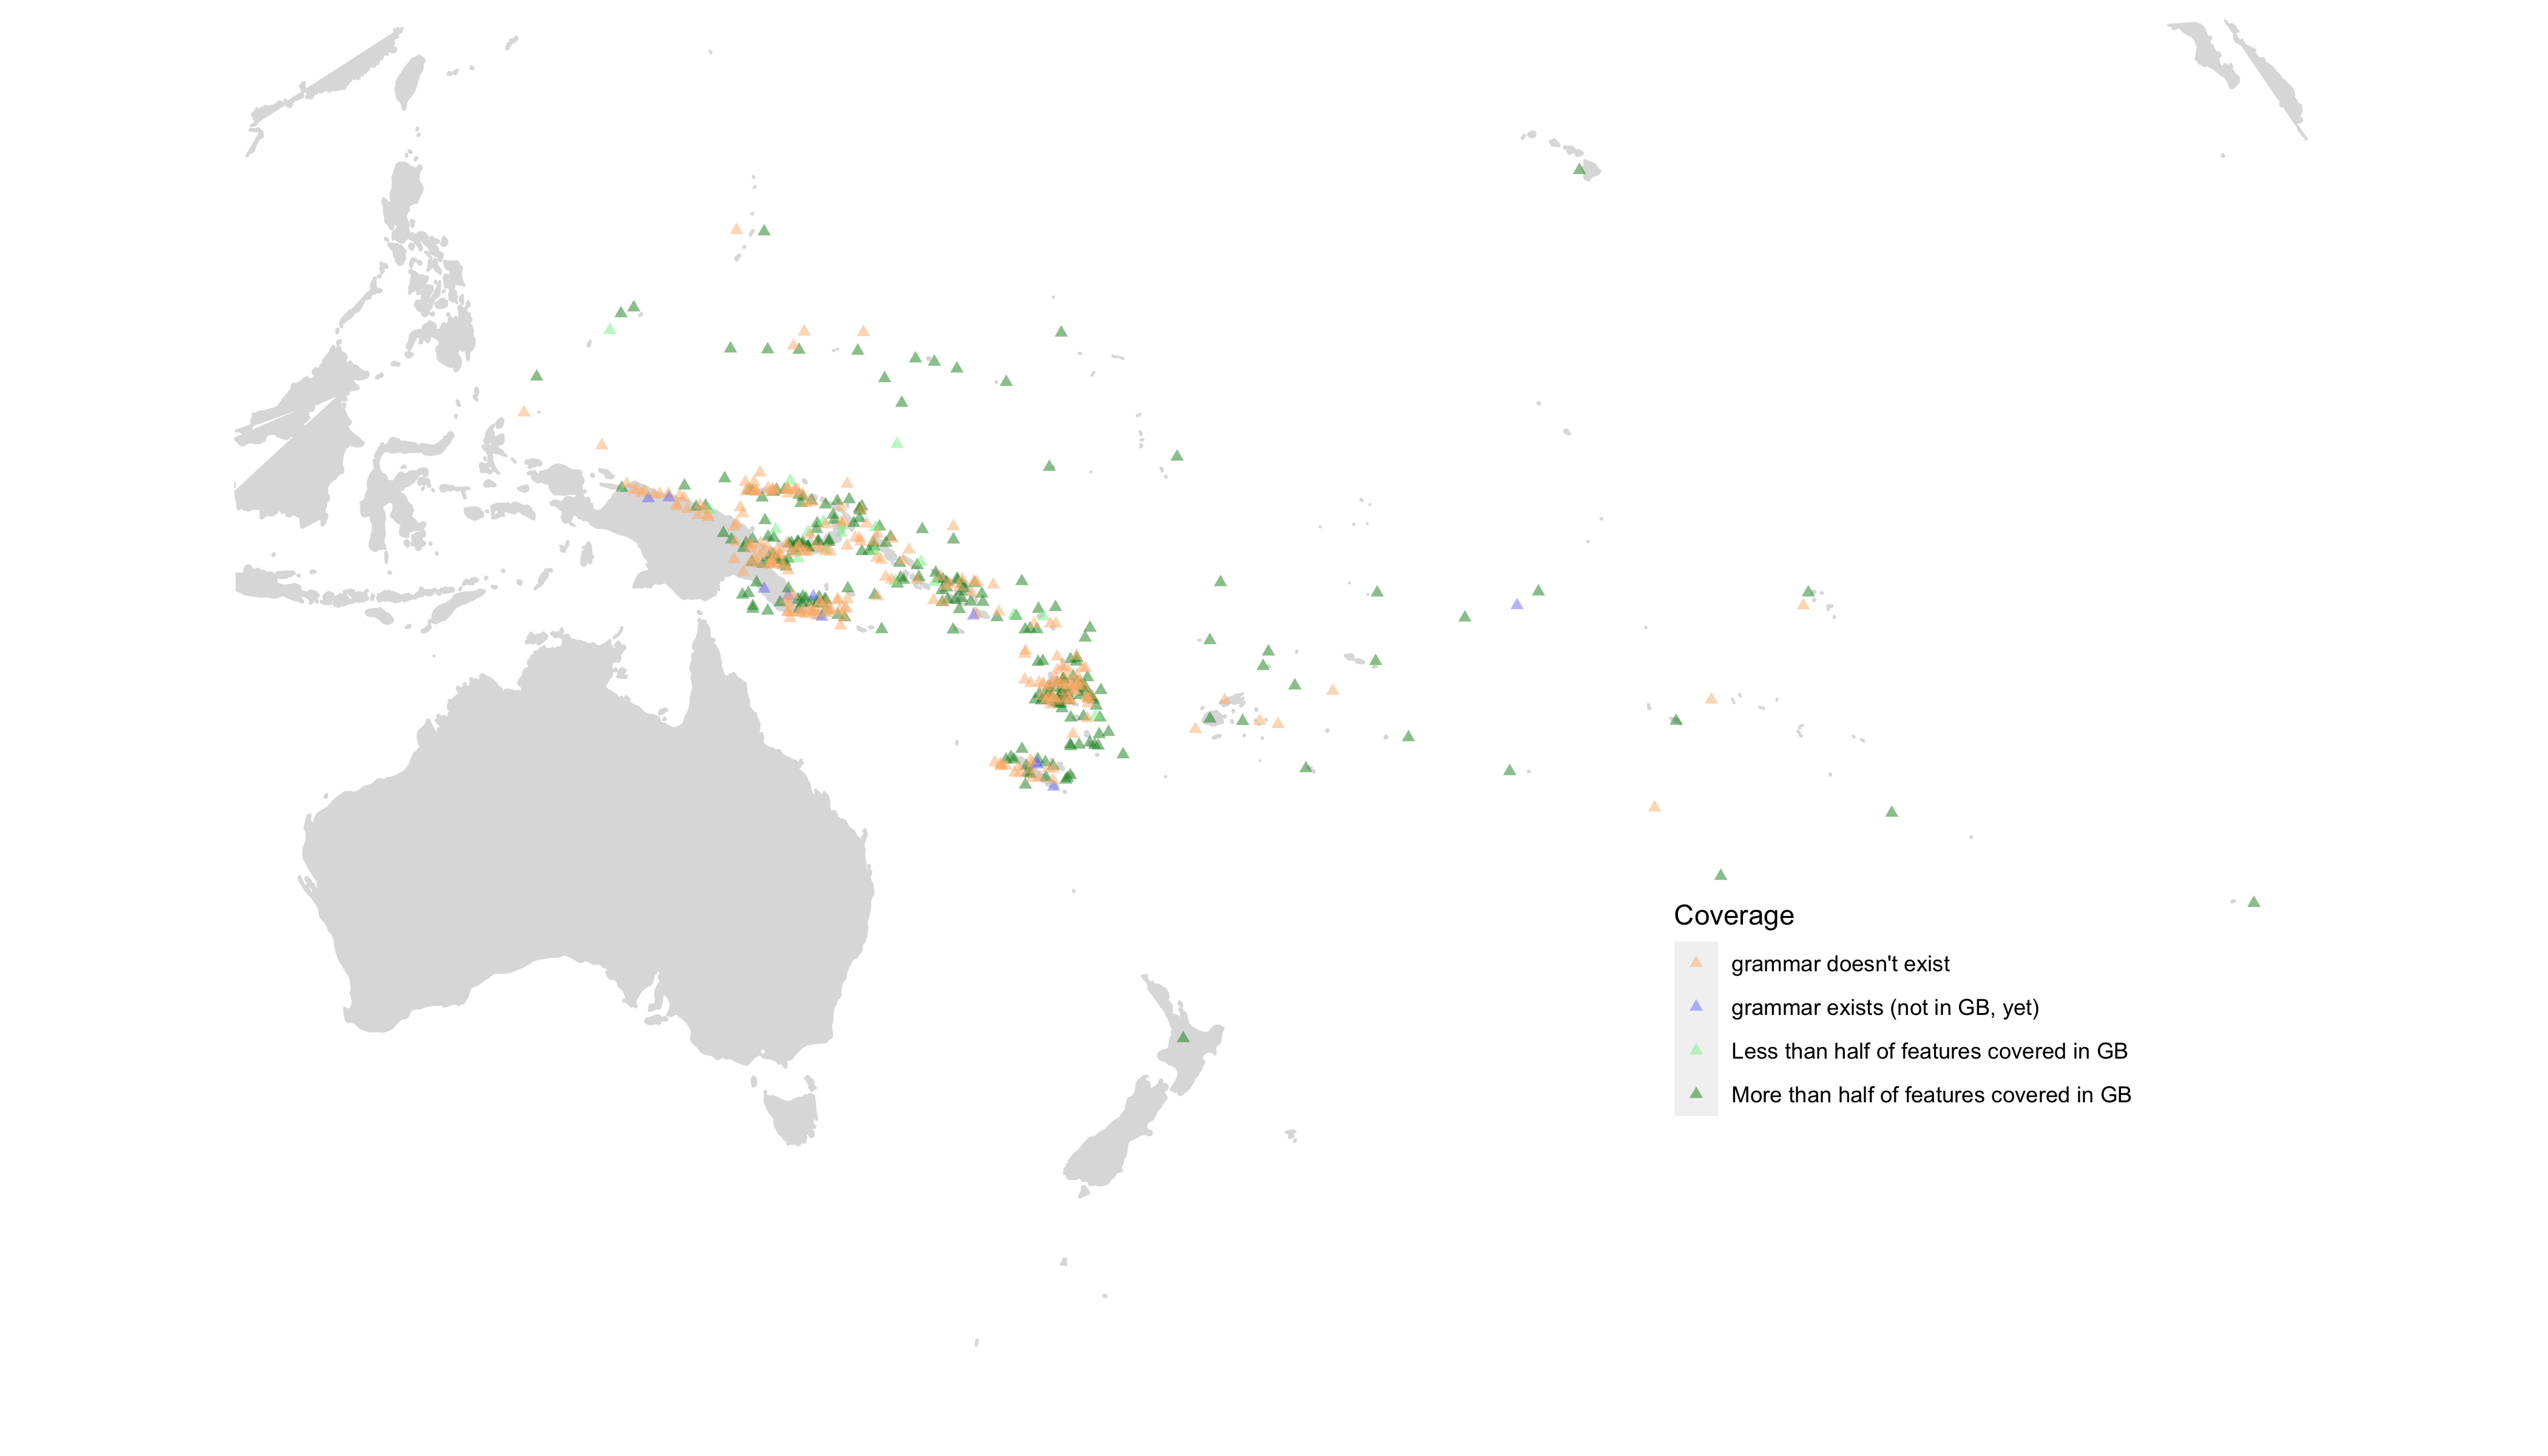
\includegraphics[width=\textwidth]{illustrations/plots_from_R/coverage_plots/maps/coverage_map_oceanic.png}
\caption{Map of Oceania, with Oceanic languages coloured for their coverage in Grambank.}
\label{GB_austro_coverage}
\end{sidewaysfigure} %#update

The coverage of Grambank data for the Oceanic subgroup is in general better in the east than in the west. However, since we control for genealogical relatedness in our ASR with trees directly, this is less of a problem for our methodology than if we were using traditional probability sampling (c.f. \citet{ross2004morphosyntactic}).

\FloatBarrier
\subsubsection{The trees}
\label{the_trees}
The tree phylogenies used in this study are: 

\begin{enumerate}[label=(\alph*)]
    \item the Maximum Clade Credibility Tree (MCCT) from \citet{grayetal_2009}
    \item a random sample of 100 posterior trees from \citet{grayetal_2009} 
    \item the tree from Glottolog 4.5\footnote{The tree of Glottolog 4.5 \citep{glottolog4_5} is based on work by \citet{blust_2009, blust_2014} and \citet{blust_chen_2017}.}
\end{enumerate}

Figure \ref{tree_coverage_oceanic_gray} and Figure \ref{tree_coverage_oceanic_glottolog} show the Grambank coverage of languages over the phylogenies from the Gray et al 2009-MCC-tree and the Glottolog-tree respectively. 

\begin{figure}[ht]
\centering
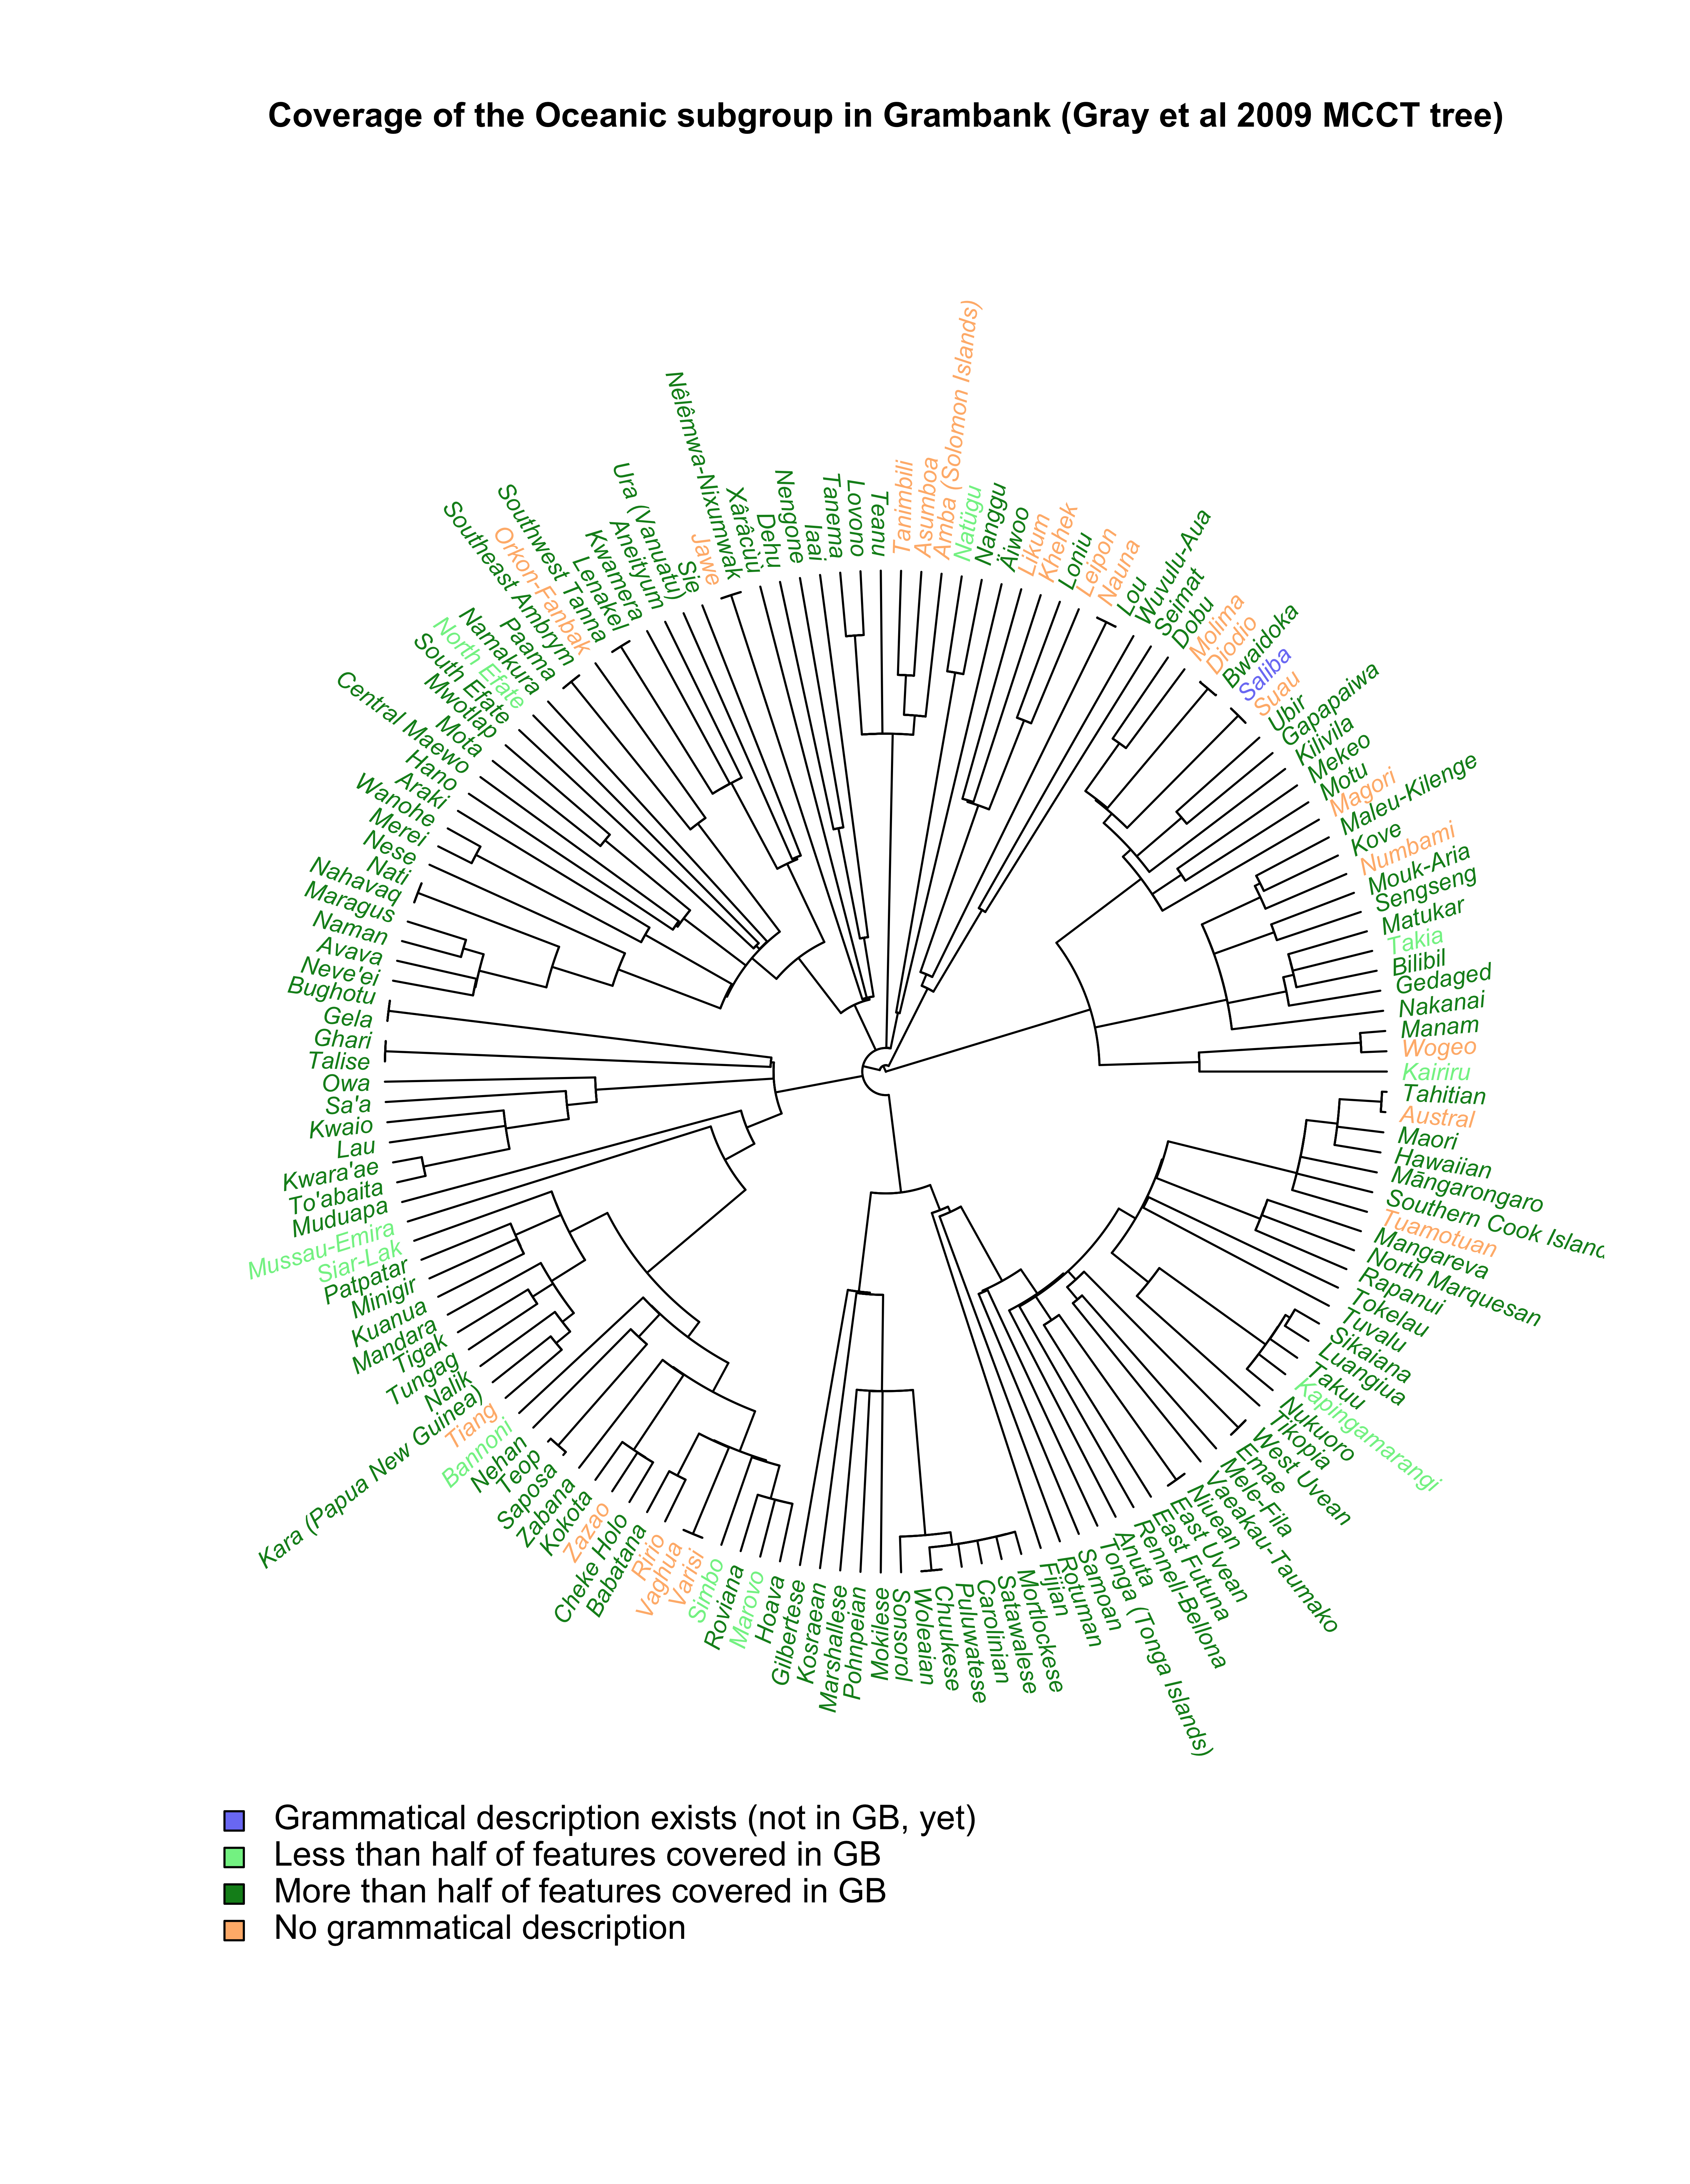
\includegraphics[width=\textwidth]{illustrations/plots_from_R/coverage_plots/tree/Oceanic_tree_desc_status_gray_et_al_tree_mcct.png}
\caption{{Maximum Clade Credibility Tree of Oceanic from \citet{grayetal_2009}, with languages coloured for coverage in Grambank.}}
\label{tree_coverage_oceanic_gray}
\end{figure}

\begin{figure}[ht]
\centering
\includegraphics[width=\textwidth]{illustrations/plots_from_R/coverage_plots/tree/Oceanic_tree_desc_status_glottolog_tree.png}
\caption{\textbf{Tree of Oceanic from Glottolog, with languages coloured for coverage in Grambank.}}
\label{tree_coverage_oceanic_glottolog}
\end{figure}

One of the major differences between the trees is that the Glottolog-tree does not contain \emph{any} information on branch lengths. All the branches in the Glottolog-tree are of the same length (1), whereas the branches in the Gray et al 2009-trees (the MCCT and the posteriors) have meaningful branch lengths based on rates of change in the underlying data (basic vocabulary) and calibration points (archaeological dates). This can be seen in the visualisations in Figures ~\ref{tree_coverage_oceanic_gray} and \ref{tree_coverage_oceanic_glottolog} where the first has varying lengths of branches but the latter all have a uniform length (1). This has the consequence that some tips in the Glottolog-tree are \emph{much further} from the root than others. This is a big disadvantage with this type of tree, since it suggests that different amounts of time has passed between the root and the languages at the tips. 

In addition, the Glottolog trees contains more non-binary splits (polytomies) than the \cite{grayetal_2009}-trees. Binary splits ought to be more plausible, since it is unlikely that a set of 3 or more languages are all \emph{exactly} equally related to each other. Polytomies can be a way of signalling uncertainty, when it is not clear how to structure the group it may be preferably to suggest a polytomy than a less certain binary branching. In the Glottolog Oceanic tree (pruned for matches to Grambank), 10\% of splits are not binary. In the \cite{grayetal_2009} MCC-tree, only 3\% are non-binary. Taking into account samples from the posterior is another way of accounting for uncertainty without needing polytomies as much. In the random sample of 100 trees from the \cite{grayetal_2009} posterior 39 trees had binary splits, the mean percentage of non-binary splits across all 100 is 0.15\%. Further technical details of the trees can be found in Supplementary Material \ref{supp:tree_details}.

The Glottolog-tree contains all the languages in the Oceanic subgroup. Therefore the coverage per island group that is summarised in table ~\ref{GB_coverage_table_island_group} in the previous section applies to the Glottolog-tree as well. However, the \cite{grayetal_2009}-trees do not contain all Oceanic languages, but rather 155. Out of these, 132 also occur in the Grambank dataset. %A breakdown of coverage for the\cite{grayetal_2009}-trees per island group is found in table ~\ref{GB_coverage_table_island_group_gray}.

Finally, we are also using a sample of the posterior trees from \cite{grayetal_2009}. Their study yielded 4,200 posterior trees. Tree topologies that are more probable occur more often. By using a set of possible trees instead of just one we may be able to include diverging historical accounts, which could for example estimate contact events as well as inheritance. Figure ~\ref{densitree_plot} shows a DensiTree-visualisation \citep{bouckaert2014densitree} of the 100 trees which are used in this study.

\begin{figure}[ht]
\centering
\includegraphics[width=18cm]{illustrations/plots_from_R/coverage_plots/tree/gray_et_al_2009_100_sample_densitree.png}
\caption{\textbf{DensiTree \citep{bouckaert2014densitree} visualisation of the 100 random sampled trees from the Gray et al 2009-posterior.} Made with the function densiTree() from the R-package Phangorn \citep{phangorn}.}
\label{densitree_plot}
\end{figure}


\FloatBarrier
\subsubsection{Data from historical linguistics on Oceanic proto-language grammar}
\label{sec:POC_lit_review}

%The Oceanic subgroup is well-studied in historical linguistics, in particular its lexicon (see the book series on the Proto-Oceanic lexicon \citep{protooceanicvol1, protooceanicvol2, protooceanicvol3, protooceanicvol4, protooceanicvol5}, among other publications). There has also been considerable work done on reconstructing the grammar of proto-languages, in particular Proto-Polynesian. See table \ref{HL_prediction_table_summary} in section \ref{sec:POC_lit_review} for a summary of all the sources consulted from classical historical linguistics.

Oceanic proto-languages are well-researched in terms of their lexicon and phonology compared to most languages in the world (see the book series on the Proto-Oceanic lexicon \citep{protooceanicvol1, protooceanicvol2, protooceanicvol3, protooceanicvol4, protooceanicvol5}, among other publications). There exists also substantial work done on the grammar of Proto-Oceanic using conventional methods in historical linguistics. We have summarised several major works in the field and distilled their research into predictions about Grambank variables in proto-languages. This section gives an overview of the works included and examples of how they have been incorporated into the study. Table~\ref{HL_prediction_table_summary} in the supplementary material \ref{supp:proto_lg_coding_table} lists all of the publications used here as representations for the reconstruction of grammar in Oceanic linguists by conventional historical linguistics means.

For each of these publications on the grammar of proto-languages, findings have been extracted that support a certain coding in the Grambank Questionnaire for a given proto-language. For example, \citet[4]{marck2000_encyclo} writes that a causative prefix can be reconstructed for Proto-Polynesian (\emph{*faka-}). In the Grambank questionnaire, we have the feature GB155 `\emph{Are causatives formed by affixes or clitics on verbs?}'. For Proto-Polynesian and GB155 the predicted state from HL is``1'' (yes/presence). For simplicity, we are only considering four ancestral languages: Proto-Oceanic, Proto-Central Pacific, Proto-Polynesian and Proto-Eastern Polynesian. The choice to focus on these four, in particular, was based on the fact that they are the most well-researched proto-languages in the literature in terms of grammatical features that can be coded for in Grambank. 

%As has been discussed earlier in this paper,  ASR in historical linguistics is usually carried out with words and sounds, but it can also be applied to grammmar. ASR of grammar is controversial because it is not entirely clear what are sounds principles to base the methodology on. The main conflict concerns the nature of the data itself and how cognacy can be determined, which is a necessary precedent for analysis within the Comparative Method-framework. In this paper, we tease our specifically ASR from the toolbox of historical linguistics and borrow methods from biology and cultural evolution in regards to determining validity of the data, see the preivous section \ref{sec:is_it_valid}. 

%\citet{crowley1985common} for example traces the history of a common noun phrase marker \emph{*na/*a} in Oceanic languages and \cite{lynchrosscrowley_proto_grammar_oceanic} discuss word-orders in proto-Oceanic.

%The data in this paper does not track specific forms, as is common when reconstructing proto-languages in historical linguistics (c.f \citet{pawley1973some, crowley1985common, evans2003study}). Instead we use binary features of a typological questionnaire which tracks a large part of ``core" grammar --- the Grambank dataset. (c.f. \citet{carling2021reconstructing}) This section outlines some crucial differences between structural data and the kind of data that is typically used in historical linguistics in relation to the present study.

As evident by the example in the previous paragraph, the work on ASR of grammar in Oceanic languages typically concerns specific forms (e.g. \emph{*faka-}) while the Grambank questionnaire targets more abstract features. This means that the Grambank coding of the proto-languages based on conventional historical linguistics ASR is not a \emph{precise} rendition of the literature, but a typological interpretation of the historical research. This task is the same as the coding of the extant daughter languages (Tikopia, Paluan etc), we read grammars that describe particular forms, paradigms etc and then translate that into Grambank-datapoints. 

When doing ASR in conventional historical linguistics, scholars in this field also take into account fossilised forms (e.g. the common noun marker \emph{-a} fusing to roots in Paamese \citep[141]{crowley1985common}) and related meanings (e.g. the hypothesis of \emph{-Cia} changing from a transitivising suffix to a marker of passive voice (\citet{hale_1968, hohepa_1967, hohepa_1969, chung1978} and \citet{jonsson1998}). The Grambank dataset, however, (as many other typological surveys) only considers productive patterns and does not include information on specific formal expressions of grammatical phenomena or so-called ``fossils'' which no longer express the function productively.


% \citet{crowley1985common}, \citet{clark1973aspects}, and other schlars whose work we will compare to our results in this paper, typically apply the comparative method to specific formal expressions of structural features (the \emph{na} article, \emph{-Cia} suffix, \emph{faka-} prefix etc). 
 
%Surveys of this kind do not track forms, but abstract features such as ``Does the language mark passive voice?''. This means that two languages can be coded identically for entirely different reasons and without being related. For example, Koasati [koas1236] of Louisiana, USA, and Mokilese [moki1238] on Mwoakilloa in the Federated States of Micronesia are both coded as having a construction for predicative possession of the type ``Topic'' by \citet{wals-2011-117}. However, they belong to entirely different language families and different parts of the world. Their similarity does not necessarily imply shared inheritance. This is unlike cognacy data, where the fact that two languages have cognates in common is direct evidence of relatedness.


As an example of what it means to consider fossils, let us consider markers of definiteness in Oceanic languages. \citet{crowley1985common} investigates ``common noun phrase markers''\footnote{This term is more or less identical to a prenominal definite/specific article.} in Oceanic and finds that in many languages there is a reflex of what is taken to be proto-Oceanic \emph{*na/*a}, but that in some languages there is another marker with a different origin (M\={a}ori \emph{te} for example). In Crowley's study, languages where there is no common noun phrase marking whatsoever and those with a marker that is not cognate with \emph{*na/*a}, are both included in type 1 (see Fig.~\ref{fig:crowley_map}). These languages are contrasted with those that have retained some kind of reflex of \emph{*na/*a} (type 2-4 in Fig.~\ref{fig:crowley_map}). This means that we can distinguish languages which have retained the proto-form from those that have not, but not languages which have a common noun phrase marker from those that do not.

\begin{figure}[!ht]
\centering
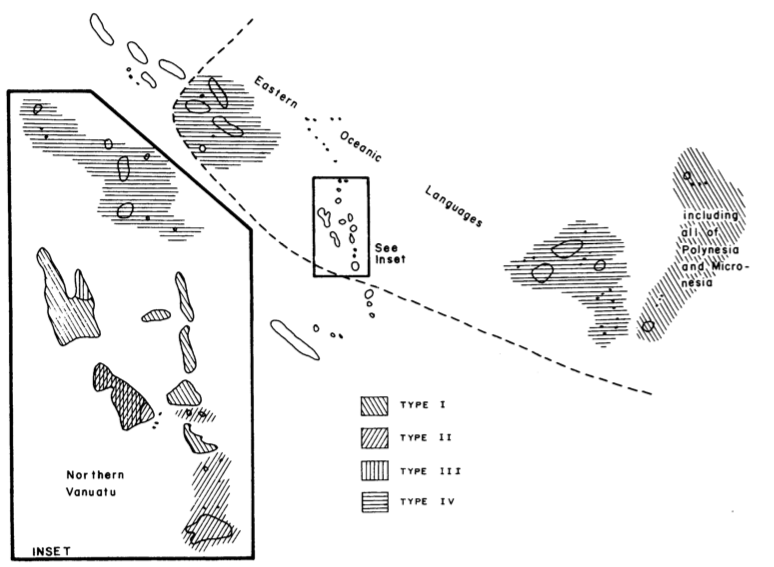
\includegraphics[width=15cm]{illustrations/crowley_1985_map.png}
\caption[Map of four different types of common noun phrase markers in Eastern Oceanic from Crowley(1985).]{\textbf{Map of four different types of common noun phrase markers in Eastern Oceanic from \citet[162]{crowley1985common}. Type 1: absence of common noun phrase marker or marker is not a reflex of \emph{*na /*a}, type 2: non-productive system involving a reflex of \emph{*na /*a}, type 3: productive marking involving \emph{*na /*a} as a prefix that is regularly separable from the noun and type 4: productive marking involving \emph{*na /*a} generally existing as a free-standing marker. Areas with cross-hatching show a distribution of both Type I and Type II systems, with definite areas being difficult to delineate on a map of this scale.}}
\label{fig:crowley_map}
\end{figure}

In contrast, the corresponding feature in Grambank is `GB022: \emph{Are there prenominal articles?'} (see Fig.~\ref{fig:gb022_map}). Languages that have \emph{te} (like M\={a}ori) or reflexes of \emph{*na/*a} as articles before the noun both count as ``yes'' (1) for GB022 and those that have no prenominal marker as a ``no'' (0). This Grambank feature splits Crowley's type 1 into two categories and combines all the languages with reflexes of \emph{*na/*a} and \emph{te} (or other markers) into one category with no distinction made for the form. We can now distinguish those that have a prenominal article from those that do not, but we cannot tell apart those which have retained the proto-form \emph{*na /*a} from those which have not. 
%Since many reconstructions of grammar in historical linguistics rely on particular forms, this is an important difference. This does not matter for features such as word order.

\begin{figure}
\centering
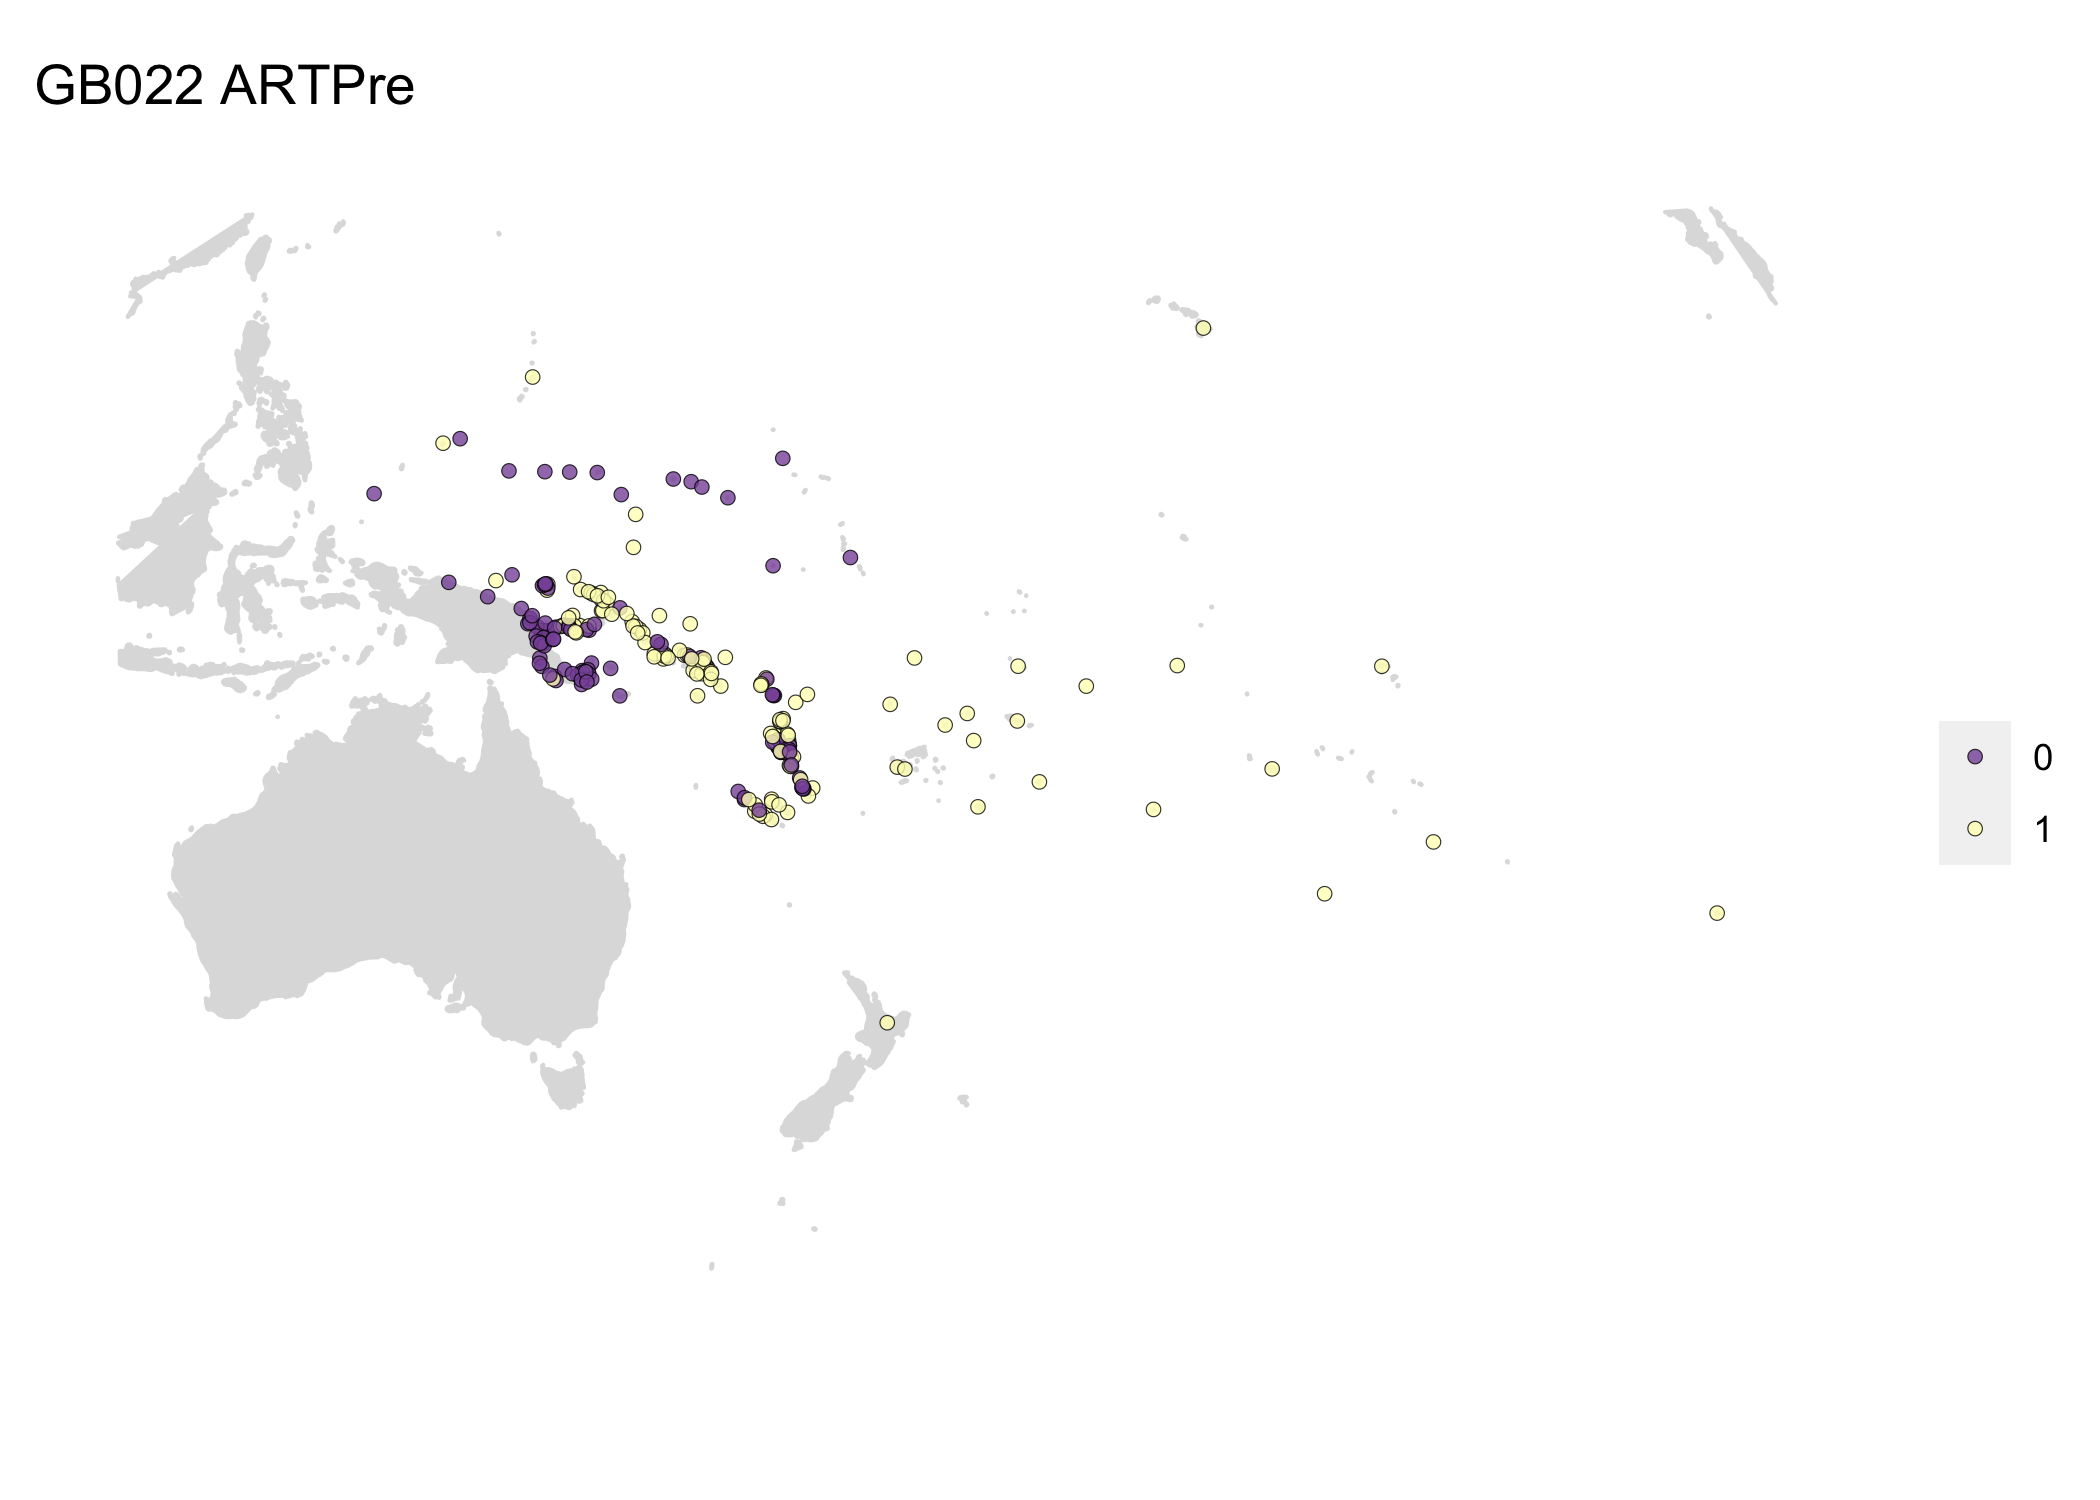
\includegraphics[width=16cm]{illustrations/plots_from_R/coverage_plots/maps/map_GB022.png}
\caption{{Map of Austronesian languages for GB022 \emph{Are there prenominal articles?} Yellow = ``yes", purple = ``no".}}
\label{fig:gb022_map}
\end{figure}

This is a difference in the kind of data that goes into the analysis, not a difference in the analytical methods themselves (compare with task a and c in fig \ref{fig:HL_tasks} respectively). 

While this principal difference is important, it should also be noted that Grambank feature GB022 have strong phylogenetic signal (negative D-estimates which are statistically similar to 0, see section \ref{sec:is_it_valid} for details). This gives us confidence that we can move ahead.

As we have seen, Grambank data is composed of abstract features such as ``is a grammatical distinction made between X and Y?''. This makes it different from most ASR-studies of grammar in historical linguistics, which tend to be more focussed on particular grammatical expressions such as morphemes. Two languages can be coded alike in Grambank and many other typological surveys, but not share ancestry. It is also possible that such abstract features track inheritance beyond the particular forms. \citet[503]{ross2004morphosyntactic} notes that a particular structure of the pronominal system of Mokilese is maintained, despite the formal markers being continuously replaced. He argues that there are discourse-related reasons for maintaining this system and that the interaction between this construction and the rest of the grammar is such that the distinction is maintained. When particular markers are lost in this system, new ones appear in their place\footnote{\citet{ross2004morphosyntactic} also notes that Goddard has observed similar patterns in Algonquian languages \citep{goddard1993algonquian}.}. This may be true of more features, and in such cases, languages can share a grammatical structure due to inheritance but not have the same particular forms. \citet[400-401]{evans2003study} also notes that while reconstructions based on lexical data are seen as more secure, they're not always possible or practical. It can be beneficial and necessary to aim to reconstruct patterns. % In addition, in many instances --- particularly within families --- abstract features such as 'GB022: \emph{Are there prenominal articles?}' are in fact correlated with specific forms even if the forms are not explicitly being tracked.

In the Grambank project, research assistants read published grammatical descriptions and extract information such that it fits with the definitions of our typological questionnaire (see Supplementary Material \ref{Grambank_features}). This survey of the literature on Proto-Oceanic grammar is essentially the same task. Just as with the literature on reconstructed languages, scholars sometimes disagree on the nature of contemporary languages and how they should best be analysed. It is up to the coder to make calls on which analysis to apply, what can be inferred from the literature and what should be left as unknown. It is possible to squeeze even more findings out of these publications; I have tended to be conservative in my interpretations the literature on Oceanic proto-languages. Out of the 201 (binarised) features in our questionnaire, 33\% (67) were answerable for Proto-Oceanic given the existing studies in historical linguistics. The average completion per language in the whole of the Grambank data set is 85\% (170). 

Overall, the literature on ASR of grammar in Oceanic suggests that Proto-Oceanic was a language with a prenominal definite/specific article \citep[136]{crowley1985common}, a distinction between inclusive and exclusive first person pronouns (\citet[112]{pawley1973some}, \citet[184]{crowley1985common}, \citet[500]{ross2004morphosyntactic}, \citet[67, 75]{lynchrosscrowley_proto_grammar_oceanic}), no gender distinctions in pronouns \citep[498]{ross2004morphosyntactic}, a dual number category in pronouns (\citet[498]{ross2004morphosyntactic}, \citet[69]{lynchrosscrowley_proto_grammar_oceanic} and \citet[173]{pawley1973some}), a distinction between alienable and inalienable possession\footnote{A distinction can be made between three different kinds of possessive classification: alienable/inalienable, direct/indirect and dominant/inactive. For the purposes of Grambank and this study, these are treated as similar enough to be included in the same category.} \citep[69]{lynchrosscrowley_proto_grammar_oceanic}, prepositions (\citet[167]{pawley1973some}, \citet[498]{ross2004morphosyntactic}), subject proclitics and object enclitics on the verb (\citet[498-499]{ross2004morphosyntactic}, \citet[83]{lynchrosscrowley_proto_grammar_oceanic}), possessive suffixes on the possessed noun (\citet[495]{ross2004morphosyntactic}, \citet[155]{pawley1973some}) and a transitivising suffix on verbs (\citet[352]{pawley1970change}, \citet[171]{pawley1973some}, \citet[80, 92]{lynchrosscrowley_proto_grammar_oceanic}). All studies cited are found in the table in Supplementary Material \ref{supp:proto_lg_coding_table},

Most of the time, the scholars of Proto-Oceanic are in agreement in their predictions. For example, \citet[142]{pawley1973some}, \citet[292]{ross2007two}, \citet[xiii, 125]{clark1973aspects} and \citet[89]{lynchrosscrowley_proto_grammar_oceanic} all propose that proto-Polynesian had a construction marking prohibitive that was different from declarative negatives. However, in some instances, there are disagreements as discussed in section \ref{sec:hl_disagreements}. In total there are 115 data points where there was either just one publication supporting the statement or if there were several they agreed. There were 3 data points where there is disagreement, these all concerned alignment of either proto-Polynesian or proto-Central Pacific.

%It is possible that differences between the computational reconstructions and those derived from conventional historical linguistics sources discussed in this section are not all related to the methodology \emph{per se}, but the coding of the patterns in languages (task 1 in \ref{fig:HL_tasks}). Reconstructions in conventional historical linguistics tend to focus on what is known as ``dominant'' or ``basic patterns''. For example, \citep[118-122]{kikusawa2002proto} discussed research on the ``basic sentence structure'' of Proto-Polynesian and Proto-Central Pacific. When describing the grammar of a language, terms like ``basic'' and ``dominant'' most often refer to patterns that have the highest frequency in corpora or show other evidence that they are the pattern that other patterns are derived from. It is possible that many word orders exist in a language, but that one is the most common and this is the material that goes into the reconstruction process. There is an important difference here to Grambank coding. Grambank coding takes into account all patterns that are grammatical and of reasonable productivity, whether or not 


%ne such case is the alignment system of Proto-Polynesian. \citet{clark1973aspects} claims that the system was ergative while \citet{hale_1968}, \citet{hohepa_1967,hohepa_1969} and \citet{chung1978} argue that Proto-Polynesian was accusative and several of the daughter languages developed ergativity later. \citet{kikusawa2002proto} and \citet{ball2007ergativity} also disagree on the alignment of Proto-Central Pacific. Because of this disagreement, the results for the computational ancestral reconstruction for Grambank features regarding the alignment of these two proto-languages are presented separately.

\FloatBarrier
\section{Results}
We are examining results from three approaches in total: a) Maximum Parsimony (MP), b) Maximum Likelihood (ML) and c) Most Common value in daughter languages (MC). For (a) and (b) we are also using three different trees: i) Glottolog, ii) \citet{grayetal_2009} MCC-tree and ii) the mean values of reconstruction of a random selection of 100 (out of 4,200) trees in the Bayesian posterior of \citet{grayetal_2009}. That gives 2 * 3 + 1 results, i.e. 7.

The results are divided up into three sections: 1) Concurrence with conventional historical linguistics, 2) new predictions and 3) disagreements among historical linguists.

\subsection{Concordance between traditional historical linguistics and computational methods}
\label{sec:results_concorance}

%The match between languages in Grambank and the Gray et al-tree is 112, meaning that results with less than 56 tips are ignored. %#update


%The full table of all predictions (excluding those relating to conflicts) and all results per feature, tree and method can be found in table~\ref{asr_table_appendic} in appendix \ref{ASR_comparison_table}. 

Table \ref{True_post_results_table} shows the number of False, Positive and Half-results for each method and tree\footnote{There was one feature for the ML method and the Gray et al 2009-trees where the computation could not be carried out because all the languages had the same value. In such cases, the function used (corHMM from the R-package corHMM \citep{R-corHMM}) gives an error because it cannot compute the rates matrix. This is why the total is 114 for ML + Gray et al 2009-trees.}. Overall all methods have a large amount of True Negative/Positive results compared to False Negative/Positive, i.e. the vast majority of the time they reconstruct the same grammatical features as suggested by traditional historical linguistics literature. One of the most striking features in Table \ref{True_post_results_table} is the large amounts of Half-results in the Most Common method --- the method where we simply count directly what is most common in all daughters. This means that there were many instances where this approach would not confidently be able to predict a presence or absence. It is precisely in such instances that a reliable tree and more sophisticated methodology are worthwhile in order to construct the previous states well --- looking at frequency alone is not sufficient.

% latex table generated in R 4.3.2 by xtable 1.8-4 package
% Thu Nov 30 15:19:36 2023
\begin{table}[ht]
\centering
\begin{tabular}{p{4cm}llllll}
  \toprule
$$\textbf{\parbox{2cm}{\raggedright Method}}$$ & $$\textbf{\cellcolor{spec_color_red!50}{\parbox{1.8cm}{\raggedright False Negative}}}$$ & $$\textbf{\cellcolor{spec_color_red!50}{\parbox{1.8cm}{\raggedright False Positive}}}$$ & $$\textbf{\cellcolor{spec_color_yellow!50}{\parbox{1.8cm}{\raggedright Half}}}$$ & $$\textbf{\cellcolor{spec_color_lightgreen!50}{\parbox{1.8cm}{\raggedright True Negative}}}$$ & $$\textbf{\cellcolor{spec_color_lightgreen!50}{\parbox{1.8cm}{\raggedright True Positive}}}$$ & $$\textbf{Total}$$ \\ 
  \midrule
ML Glottolog & 10 & 3 & 4 & 46 & 52 & 115 \\ 
  ML Gray et al (2009) - MCCT  & 9 & 2 & 9 & 43 & 51 & 114 \\ 
  ML Gray et al (2009) - posteriors  & 10 & 1 & 8 & 44 & 51 & 114 \\ 
  Most common & 5 & 0 & 16 & 46 & 48 & 115 \\ 
  Parsimony Glottolog & 8 & 2 & 4 & 46 & 55 & 115 \\ 
  Parsimony Gray et al (2009) - MCCT  & 6 & 5 & 10 & 42 & 52 & 115 \\ 
  Parsimony Gray et al (2009) - posteriors  & 7 & 6 & 4 & 43 & 55 & 115 \\ 
   \bottomrule
\end{tabular}
\caption{Table showing the amount of False Negative, False Positive, Half, True Negative and True Positive results.} 
\label{True_post_results_table}
\end{table}


Given these counts, we can calculate the concordance scores (see section \ref{result_calc_section}). These are displayed in Fig \ref{barplot_facet_results}. A score of 1 means identity with predictions of historical linguists and 0 means entirely dissimilar from them.

\begin{figure}[ht]
\centering
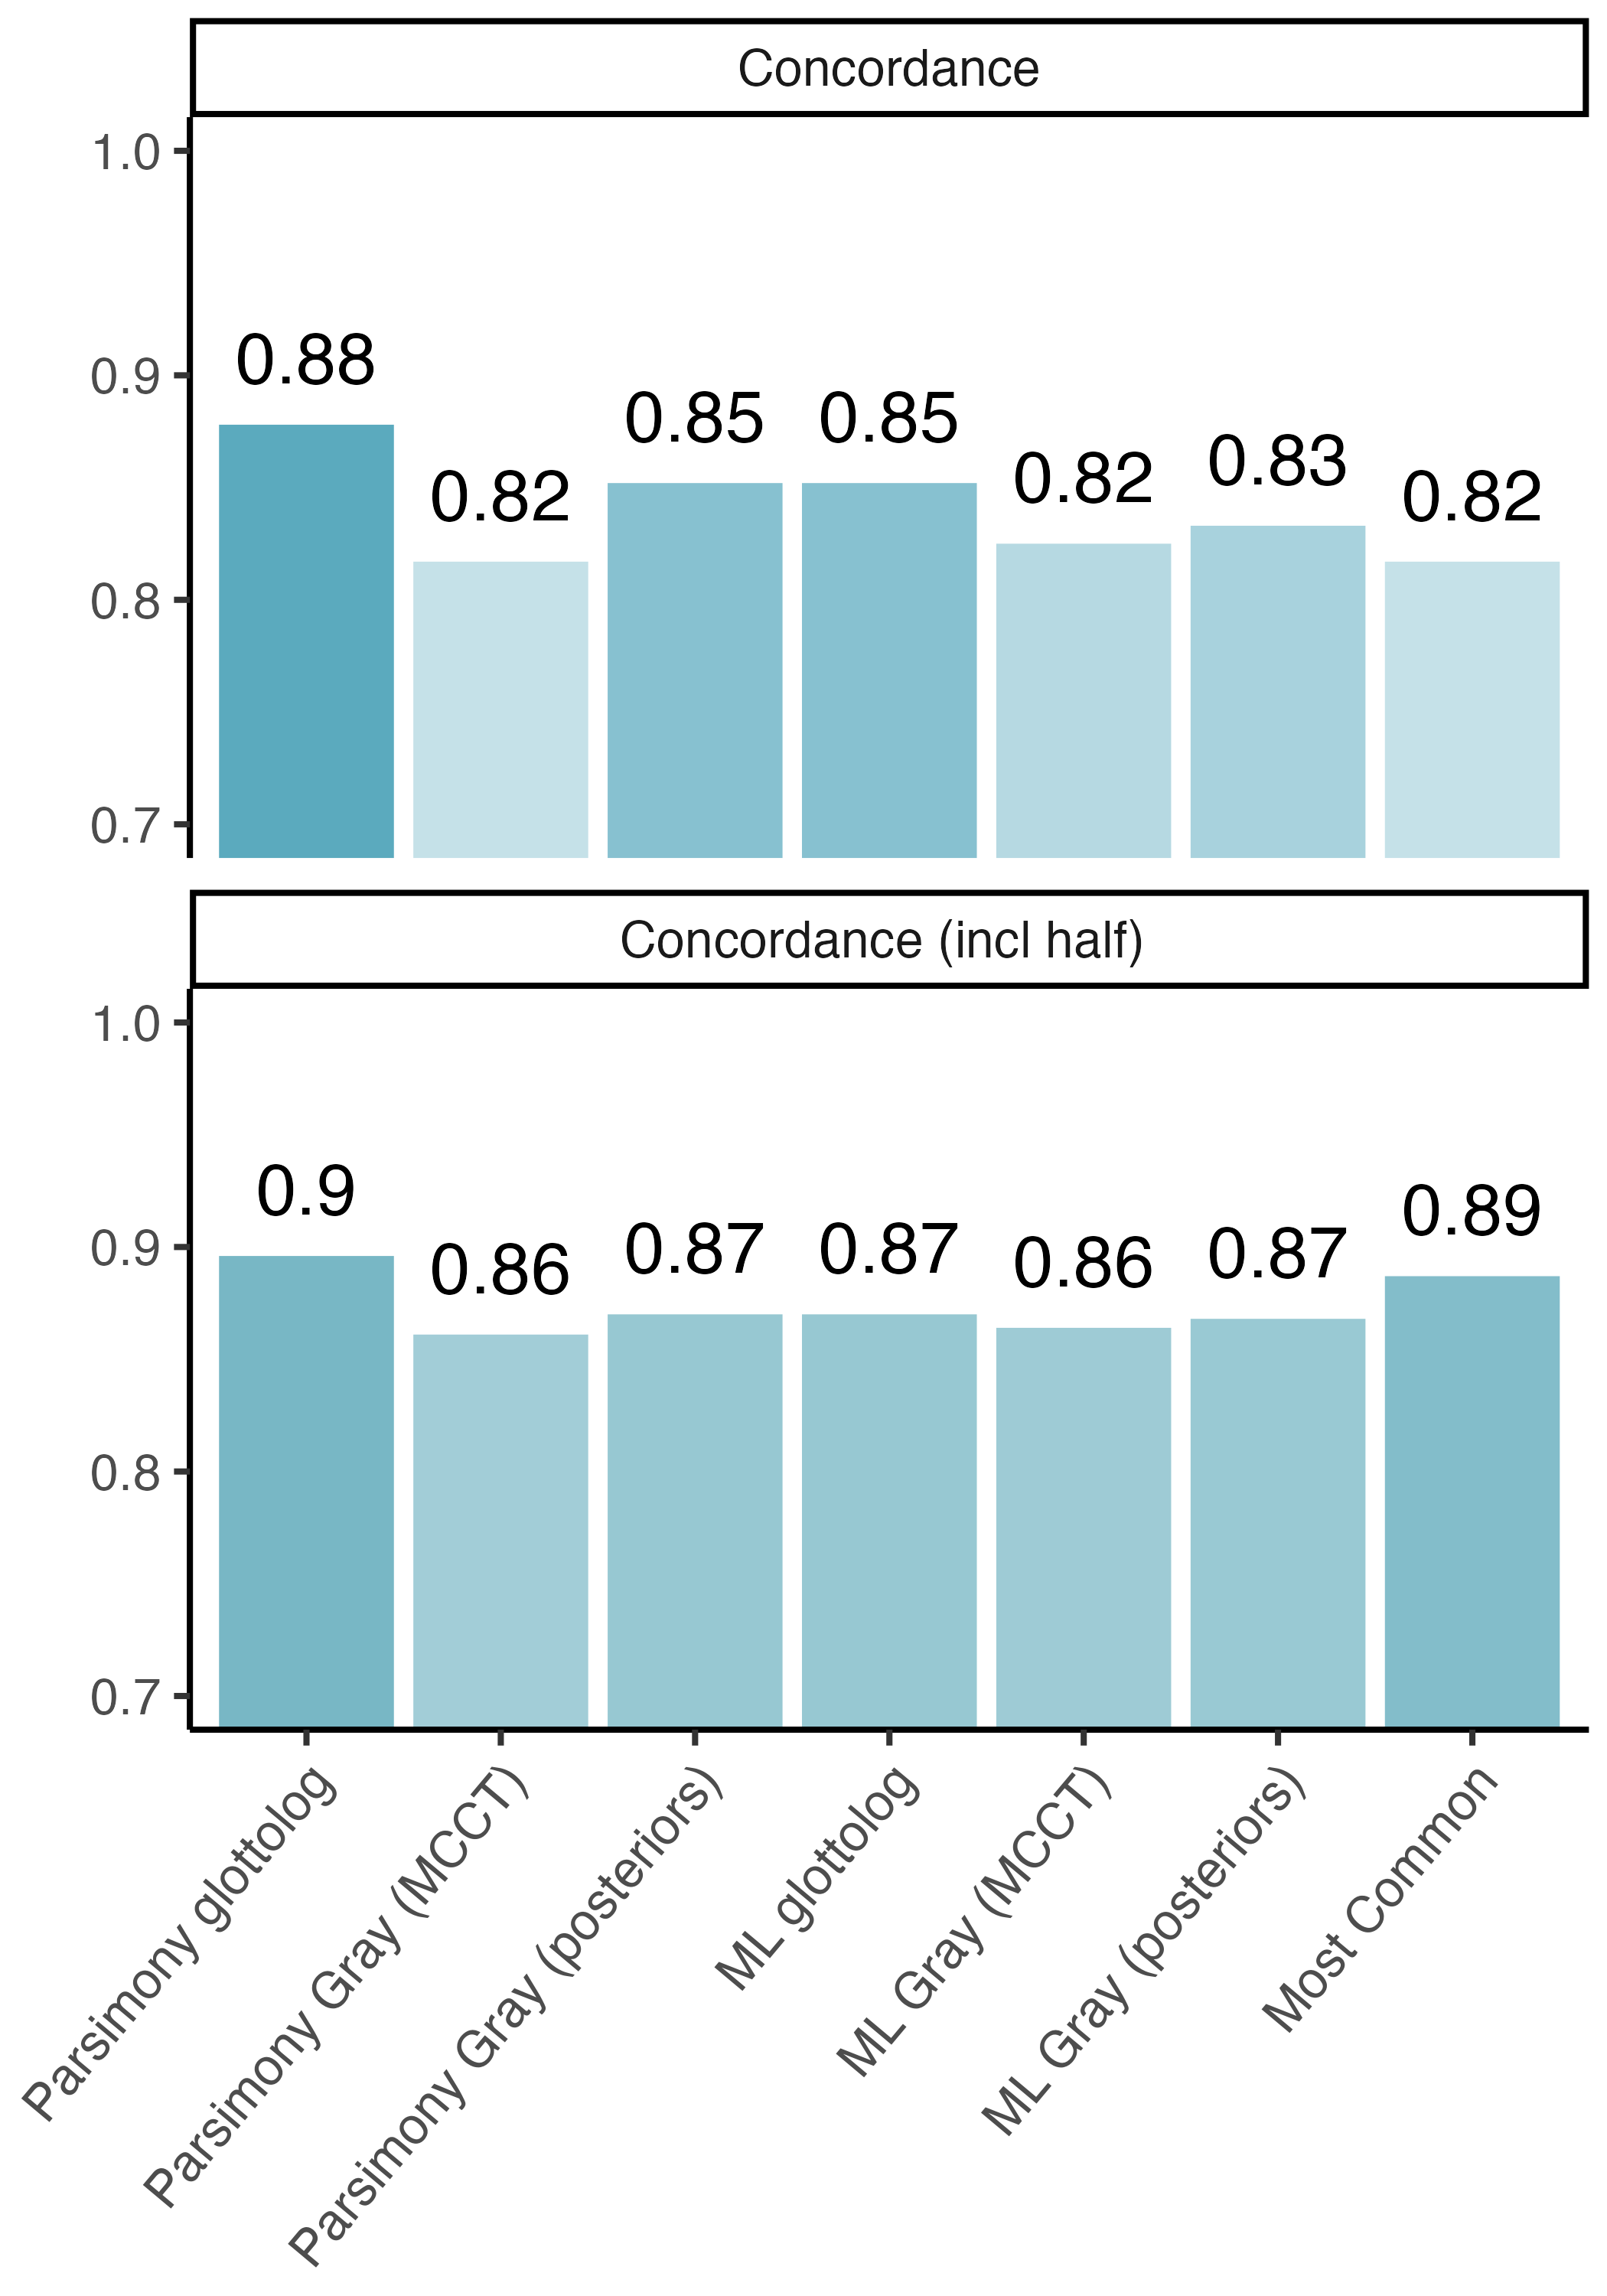
\includegraphics[width=12cm]{illustrations/plots_from_R/results/barplot_facet_scores_exclude_f1.png}
\caption{\textbf{Barplots of concordance scores of each method.}}
\label{barplot_facet_results}
\end{figure}

The inclusion of the half-results has the effect of evening out the differences between the performance of the different methods. The concordance scores which includes half-results for each method are more similar to each other.

The method that perform most similarly to historical linguists is Parsimony + the Glottolog 4.5 tree. The Glottolog 4.5 tree has a significant issue; it has no branch lengths and the topology is composed of a combination and compromise from several different sources as opposed to a principled and systematic investigation of  data. Parts of the tree are suggested by different scholars, which means that different clades are not necessarily comparable. It does have an advantage though, and that is the sheer number of languages it includes. The overlap between languages included in Glottolog 4.5 and Grambank is greater than for the \citet{grayetal_2009}-trees. It is possible that it is this sheer number of tips that gives it a greater concordance with historical linguists' predictions. The results also suggest that it is possible that historical linguists, in these specific studies, do not necessarily take into account branch lengths because there is higher agreement with the Glottog 4.5 tree (a tree without branch lengths) + the Maximum Parsimony method (a method that disregards branches altogether).

Overall, however, the methods perform similarly. There is very little that tells apart the different methods ---- they are giving very similar results and all show a high degree of agreement with conventional historical linguistics. For a more detailed example of the few cases where they disagree, please see Appendix \ref{supp:GB133_detail}.
% Out of the trees of \cite{grayetal_2009}, the random 100 posterior samples perform every so slightly better than the plain MCC-tree. This may indicate that they are possibly picking up some relevant history not represented in the MCC-tree, such as contact. The difference is very small though.

We also carried out an analysis on whether phylogenetic signal \citep{fritz2010selectivity} or the distribution of tips in either state predicts the level of agreement between each method and conventional historical linguistics (see Supplementary Materials \ref{supp:cor_d_HL} and \ref{supp:cor_min_p_HL}). The results show that there is no relationship between phylogenetic signal (as measured by the D-estimate \citep{fritz2010selectivity}) and concurrence with HL, but that there is a weak to moderate correlation with prevalence in daughter languages. If almost all languages have a given feature, HL and the computational methods tend to both reconstruct the same state. However, if the feature values varied more, however, the agreement is reduced. This is not unexpected, if most of the languages have the same profile it is not surprising that the ancestral nodes are reconstructed the same despite differing methods.

In section \ref{sec:is_it_valid} we suggested that features with D-estimates dissimilar to Brownian evolution according to the D-estimates p-values may not be suitable for ASR. The Grambank features in this category did not show any different behaviour from the rest in terms of agreement with HL (see appendix \ref{supp:cor_d_HL}), like the other features they did not show a significant correlation between agreement with HL and D-estimate. The vast majority agreed with HL. This may tell us that either a) there is no robust relationship between the agreement between methods and phylogenetic signal or b) that this particular measure of phylogenetic signal is faulty (for example that Brownian motion is not a reasonable assumption). Future studies should delve further into different kinds of measurements of phylogenetic signal and their potential applicability to linguistic data.

We can also compare the methods to each other. Fig. \ref{heatmap_accuracy_score_methods} shows the pairwise concurrence (including half-results) scores between all of the methods. All of the computational methods agree more with each other than any of them do with conventional historical linguistics. The reason is most likely related to not only the difference in methodology but also the underlying data. All of the computational methods are using Grambank data and partially the same trees, whereas the underlying language-level data in conventional historical linguistics ASR is different and the tree-structure as well. For the purposes of this study, the historical linguistics literature has been translated into Grambank data-points, but there is likely to be some discrepancy in the definitions of grammatical concepts and how to apply them to each and every language in the data-set. Reconstruction in conventional historical linguistics does not always spell out the specifics of the tree structure in terms of particular splits and branches, but is rather based on broader subgroups --- this can also be a contributing factor.

%For example, the underlying data of the map of noun markers in Oceania in Fig \ref{fig:crowley_map} from \cite{crowley1985common} 

\begin{figure}[ht]
\centering
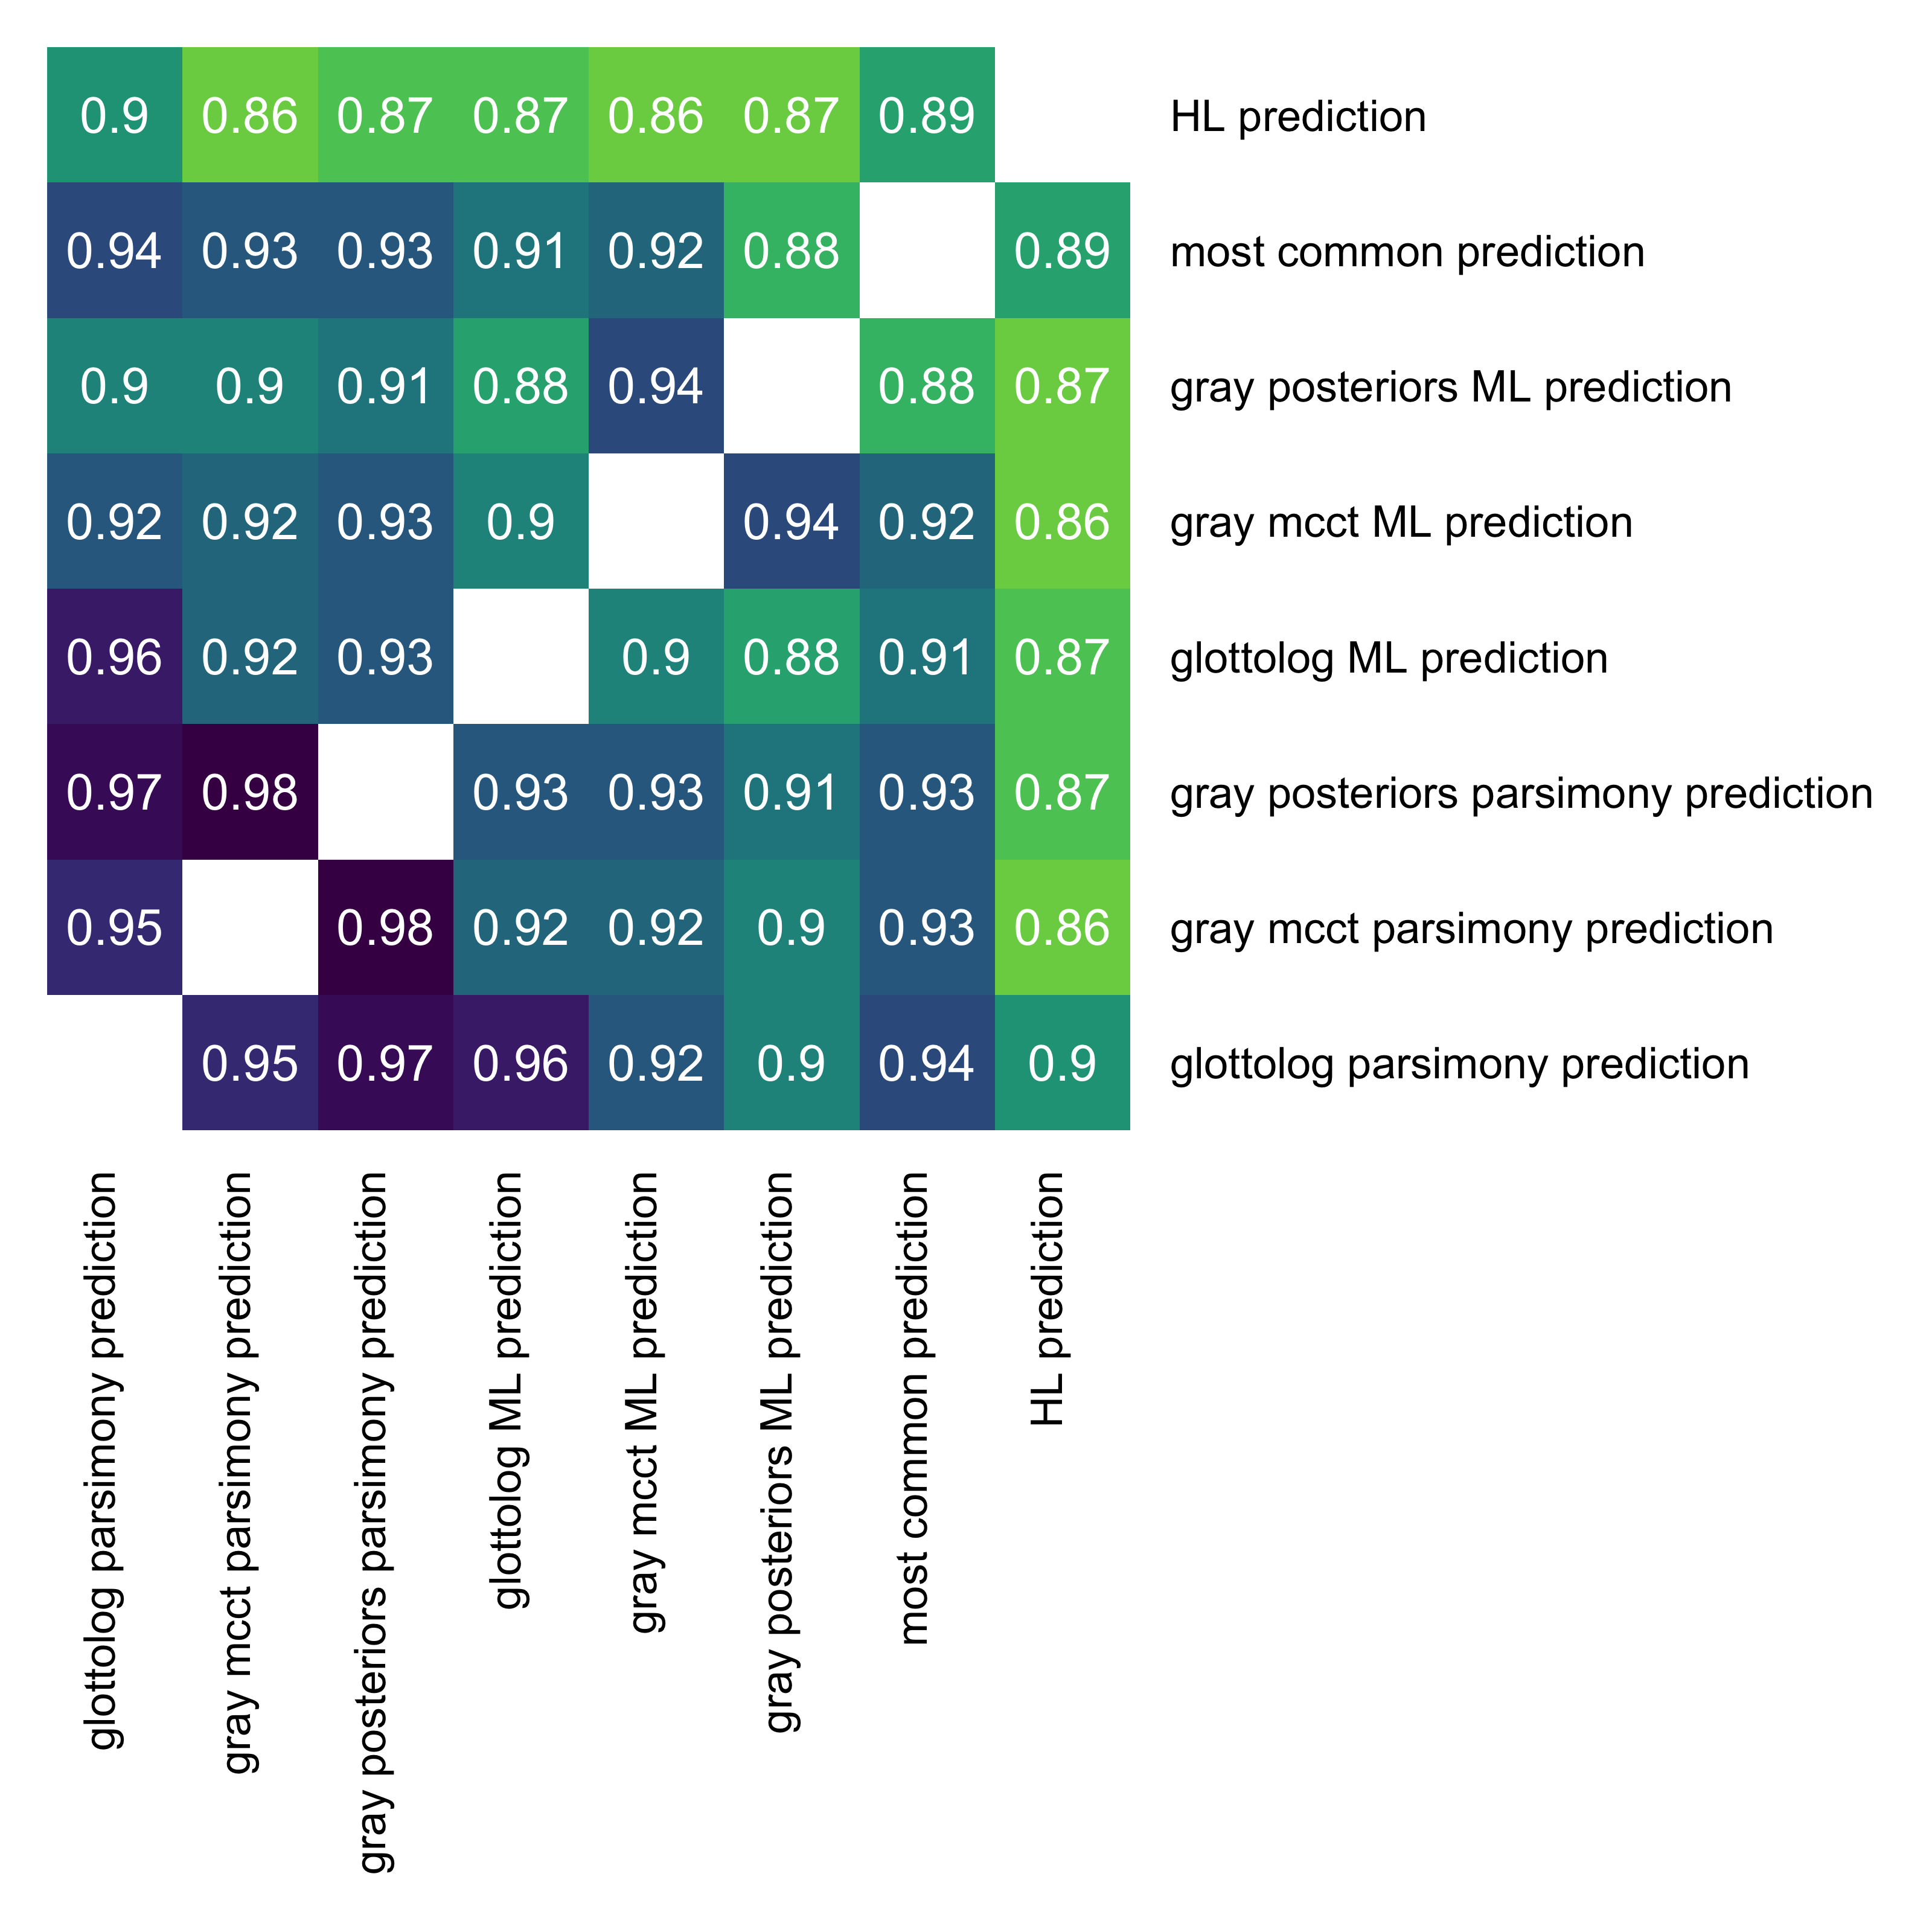
\includegraphics[width=17cm]{illustrations/plots_from_R/results/dist_heatmap_all_methods.png}
\caption{\textbf{Heatmap of accuracy score (including half) between reconstruction, per tree and method. Dark blue = high concurrence, lightgreen = low concurrence.}}
\label{heatmap_accuracy_score_methods}
\end{figure}



%As was discussed earlier, there are several different ways of evaluating the performance of these approaches. If we consider how often they made a prediction that agreed with historical linguistics out of all the times they made a confident prediction (Accuracy score excl Half/Half), then ML. If we award half a point for Half/Half predictions, Parsimony does better. However, in both instances the numbers are very close to each other.

%We are comparing our computational reconstruction results to those predicted by expert linguists. The reason that the Glottolog tree is more in line with the predictions from historical linguistics is probably because it resembles the tree most historical linguists are used to more than the Gray et al-2009 tree does (the Glottolog tree is based on \citet{blust_2009,blust_2014} and \citet{blust_chen_2017}). That is not to say it is necessarily a better reflection of the true history of these languages, but rather that it may fit better with the underlying model that the field of historical linguistics has been working with in recent decades. Most of the literature on reconstructions of Proto-Oceanic does not include detailed accounts of the exact tree topologies and branch lengths used to reconstruct the ancestral languages. As was shown in section \ref{sec:asr_methods}, we had to impute branch lengths for the Glottolog-tree. The manner by which reconstructions are postulated in historical linguistics is typically by considering how well distributed the phenomena are over certain genealogical and areal subgroups. If the distribution is convincingly non-random and the comparative method can be used to reconstruct forms, predictions about the proto-language are made (c.f. \citet[109-110]{pawley1973some}).

%Furthermore, there were fewer matches between languages for which there is Grambank data and the Gray et al Tree, making for more uncertainty in predicting ancestral states.

%In a similar study, \citet{jager2018using} attempt to reconstruct cognate classes for the proto-languages of three different language families. They used various approaches: binarising versus not binarising data; Maximum Parsimony versus Maximum Likelihood Estimation versus Minimal Lateral Networks; and using a single consensus tree versus sampling several from the tree posterior. The highest F1-score they achieved in this paper was 0.79 for the Maxmimum Likelihood Estimation reconstruction of Austronesian (using either a single tree or a sample of trees). This means that all of our results above perform ``better''. While this may be pleasing, it is not yet entirely clear why this is. 

%e were also somehow easier to reconstruct, and if so that would explain the higher F1-scores.
%\label{sec:ars:metod:hist}

%Many of the features that have been reconstructed for proto-languages of the Oceanic subgroup are also very common among Oceanic languages. For example, in our dataset 223 languages have a distinction between alienable and inalienable possession, and three do not have this feature. It is perhaps no surprise that historical linguists, Maximum Parsimony and Maximum Likelihood  agree that it is likely that the proto-languages have this feature as well\footnote{There was one exception. Maximum Likelihood on the Glottolog tree did not confidently predict presence of alienablity possession for Proto-Oceanic, the result was classified as ``half''. It did however predict alienablity for Proto-Polynesian.}. However, it is not always so simple. If this was all there was to it, we could just use raw distributions to reconstruct features of proto-languages. Historical linguists stress the importance of Maximum Parsimony and plausibility in their reconstructions, and as we saw in Fig. \ref{fig:clark_tree} (section \ref{sec:ars:metod:hist}), raw distributions alone can be misleading --- it is essential to take into account the tree structure. For example, \citet[118]{pawley1973some} suggests that verb-final word orders may have been possible in proto-Oceanic. This is tracked by feature GB133 \emph{`Is a pragmatically unmarked constituent order verb-final for transitive clauses?'}, and most languages are marked as `no' for this feature. However, Maximum Likelihood and the Gray et al 2009-tree did reconstruct presence of this feature at the root. 108 of the tips of this tree were absent, and 7 present, and yet the result was presence for Proto-Oceanic. This is (partially) due to the particular tree structure, where the languages with this feature attach further up in the tree structure (see Fig. \ref{GB133_tree_ML_gray})\footnote{It should be noted that the Maximum Parsimony result for the same tree did not reconstruct presence at the root. This has to do with the way Maximum Likelihood takes into account the distribution across the tree in each reconstruction, which gives the ancestral node of Maleu-Kilenge [male1289] and Kove [kove1237] a higher change of presence than it would under Maximum Parsimony.}\textsuperscript{,}\footnote{The languages with a presence for this feature are also mostly on the island of New Guinea and it is possible that this is a result of contact with non-Austronesian languages, as anonymous examiner 3 kindly pointed out.}.

%\newpage
%\begin{figure}
%\centering
%%%\includegraphics[width=\textwidth]{illustrations/plots_from_R/ML_gray_-GB133.png}
%\caption[Ancestral state reconstruction on tree for feature GB133, Gray et al 2009-tree and Maximum Likelihood.]{\textbf{Ancestral state reconstruction on tree for feature GB133, Gray et al 2009-tree and Maximum Likelihood. Yellow = presence, purple = absence.)}}
%\label{GB133_tree_ML_gray}
%\end{figure}
%

%
%It is often as revealing to study where the results got it ``wrong'' as where it was ``right''.Table~\ref{ASR_comparison_worst_table} shows the results for the automatic reconstructions that agreed the least with findings from classical historical linguistics. 
%
%%The two parsimony sets of results did propose that Proto-Oceanic did not have tense marking bound to the verb (GB082-GB084), nor is it by an inflecting word (GB121). However, when it came to tense marking by a particle and the aspect and mood marking, the automatic reconstructions were among the most dis-concordant with the expert predictions out of the entire dataset. In the Grambank dataset, we make a distinction between TAM-markers bound to the verb and free-standing markers that inflect versus those that don't. One possible factor that could have contributed to this is that TAM-markers in Oceanic languages are often described as forming portmanteau markers with subject markers. However, there is variation in how authors of grammars express this in their publications, and possibly also how our coders interpret the situation. This requires further investigation, which is unfortunately outside the scope of this study.
\FloatBarrier
\subsection{New predictions}
Besides the predictions made by historical linguists, we can also explore what else has strong support in our computational reconstructions that is not explicitly mentioned in the literature (see supplementary material \ref{supp:proto_lg_coding_table}). There are 111 features that are predicted as present in the four proto-languages by the two methods (MP and ML) with all three trees (Glottolog, Gray et al 2009 MCCT and ditto posteriors); i.e. 6 times. For example, they propose that Proto-Oceanic has inclusory constructions, Proto-Central Pacific uses verbs for admoninal property attribution (``adjectives'') and Proto-Polynesian has numeral classifiers. 107 of these 111 predictions were also the Most Common in the daughter languages, meaning that more than 60\% of the languages possessed the trait. There is therefore perhaps little surprise that all the methods agree. However, there are 4 cases where both MP and ML (for all three trees) agree on the presence of a particular Proto-language structural feature despite it not being the most common (see table \ref{table_extra_predictions_four}). This is where the tree structure comes into play and adds information beyond frequencies.

% latex table generated in R 4.2.2 by xtable 1.8-4 package
% Mon Mar 20 23:28:44 2023
\begin{table}[ht]
\centering
\begin{tabular}{p{2cm}p{4cm}p{8cm}}
  \hline
\$$\backslash$textbf\{Feature\}\$ & \$$\backslash$textbf\{Proto-language\}\$ & \$$\backslash$textbf\{Name\}\$ \\ 
  \hline
GB024b & Proto-Eastern Polynesian & Is the order of the numeral and noun N-Num? \\ 
  GB093 & Proto-Central Pacific & Can the P argument be indexed by a suffix/enclitic on the verb in the simple main clause? \\ 
  GB421 & Proto-Central Pacific & Is there a preposed complementizer in complements of verbs of thinking and/or knowing? \\ 
  GB433 & Proto-Central Pacific & Can adnominal possession be marked by a suffix on the possessed noun? \\ 
   \hline
\end{tabular}
\caption{Table showing the four Grambank features that were predicted as present by ML and MP in all three trees, but were not the most common feature in all languages.} 
\label{table_extra_predictions_four}
\end{table}




%Many of these are probably not surprising to most historical linguists working on Oceanic languages, but they were not explicitly predicted in the sources surveyed for this study.

%three out of the four sets of results predicted that the order of numeral and noun is N-Num, all tests supported that ``adjectives'' in Proto-Central Pacific behaved like verbs when used predicatively, and all tests also supported that Proto-Polynesian had three or more distance contrasts among demonstratives. 
\FloatBarrier
\subsection{Where the conflicts are: Ergativity}
The nature of the alignment system of Proto-Polynesian and Proto-Central Pacific is contested (see section \ref{sec:hl_disagreements}).
%\citet{clark1973aspects} posits, primarily on the basis of Maximum Parsimony, that Proto-Polynesian was ergative whereas \citet{hale_1968}, \citet{hohepa_1967,hohepa_1969}, and \citet{chung1978} argue that it was accusative (while they suggest different historical pathways, they agree that Proto-Polynesian was nominative-accusative). 

Grambank has two features that pertain to these disagreements:

\begin{itemize}
\item GB408 \emph{Is there any accusative alignment of flagging?}
\item GB409 \emph{Is there any ergative alignment of flagging?}
\end{itemize}

It is entirely possible for a language to be entered into the database as ``yes'' for both of these, i.e., from the perspective of Grambank languages are not wholly ``ergative'' or ``accusative'' --- they can have both ergative and accusative flagging simultaneously. This makes it possible for us to prove both Chung and Clark ``right'', the results can come out such that Proto-Polynesian had both accusative \emph{and} ergative alignment flagging. Table \ref{conflict_table} shows a summary of the predictions from the different historical linguists in regard to the alignment of Proto-Polynesian and Proto-Central Pacific.

\newcommand{\pb}[1]{\parbox[t][][t]{1\linewidth}{#1} \vspace{3.5pt}}

%label = conflict_table
% latex table generated in R 4.3.0 by xtable 1.8-4 package
% Fri Jun  9 18:17:42 2023
\begin{table}[ht]
\centering
\begin{tabular}{p{0.25\linewidth}p{0.2\linewidth}p{0.2\linewidth}p{0.2\linewidth}}
  \toprule
$\textbf{\pb{ Proto-language}}$ & $\textbf{\pb{ Feature ID}}$ & $\textbf{\pb{ Prediction}}$ & $\textbf{\pb{ Source}}$ \\ 
  \midrule
Proto-Polynesian & GB408 & Present & \cite[261-261]{chung1978}, \citet{ball2007ergativity} \\ 
  Proto-Polynesian & GB408 & Absent & \citet[106-107]{clark1973aspects} \\ 
  Proto-Polynesian & GB409 & Absent & \cite[261-261]{chung1978} \\ 
  Proto-Polynesian & GB409 & Present & \citet[106-107]{clark1973aspects} \\ 
  Proto-Central Pacific & GB409 & Present & \citet[1]{kikusawa2002proto} \\ 
  Proto-Central Pacific & GB409 & Absent & \citet{ball2007ergativity} \\ 
   \bottomrule
\end{tabular}
\caption{Table showing the features where historical linguists disagree.} 
\label{conflict_table}
\end{table}


The results in fact come out strongly in favour of the proposal by Clark. Table \ref{conflict_results_table} shows that MP, ML and MC all reconstruct presence for ergative flagging in Proto-Polynesian. On the matter of nominative-accusative marking, there is disagreement with the MP results all suggesting absence but the ML and MC giving a half-result.


%label = conflict_results_table
% latex table generated in R 4.3.0 by xtable 1.8-4 package
% Fri Jun  9 18:17:42 2023
\begin{table}[ht]
\centering
\begin{tabular}{p{0.25\linewidth}p{0.24\linewidth}p{0.24\linewidth}p{0.24\linewidth}}
  \toprule
$\textbf{\pb{Method}}$ & $\textbf{\pb{ GB408$\newline$Proto-Polynesian}}$ & $\textbf{\pb{ GB409$\newline$Proto-Central Pacific}}$ & $\textbf{\pb{ GB409$\newline$Proto-Polynesian}}$ \\ 
  \midrule
parsimony$\newline$Glottolog (4.4) & Absent & Absent & Present \\ 
  parsimony$\newline$gray mcct & Absent & Absent & Present \\ 
  parsimony$\newline$gray posteriors & Absent & Absent & Present \\ 
  ML$\newline$Glottolog (4.4) & Absent & Absent & Present \\ 
  ML$\newline$gray mcct & Half & Absent & Present \\ 
  ML$\newline$gray posteriors & Half & Absent & Present \\ 
  Most common & Half & Present & Present \\ 
   \bottomrule
\end{tabular}
\caption{Table showing the computational results for the features where historical linguists disagree.} 
\label{conflict_results_table}
\end{table}


As was noted earlier in section \ref{sec:POC_lit_review}, the computational reconstructions differ from those arrived at through the conventional ASR in historical linguistics primarily because the data used in this study is abstract presence or absence of structural features whereas historical linguists use specific concrete forms instead (c.f. \citet{crowley1985common}). Besides the parsimony principle (as laid out by \citet[19]{clark1973aspects} for example), expert historical linguists also take into account the plausibility of the proposed proto-language and the chain of changes posited \citep{chung1977aspects}. It is not possible for the computational reconstructions to take these assumptions into account without having them formally described and introduced into the model, which is not possible at this time. This may be the reason for the lack of support for Chung's theory; the crucial information that underpins it is not accounted for in the analysis.

Given the topology of the trees used in this study, where the ergative flagging language Tongan is always attached to the Proto-Polynesian root at a higher level than Eastern Polynesian languages (c.f. Fig \ref{poly_GB409_tree}), it is very likely that GB409 would be reconstructed as present for Proto-Polynesian. As Clark pointed out, it is the most parsimonious solution. However, it could still have been the case that GB408 (accusative) would have been reconstructed for Proto-Polynesian. The reasons for this may lie in different definitions of what counts as nominative-accusative or neutral in different descriptions, and/or plausibility of changes/states. As has been discussed earlier, it was not possible to include plausibility as a factor in this study.

The proposals of \citet{hale_1968}, \citet{hohepa_1967, hohepa_1969}, and \citet{chung1978} also involve the reconstruction of passive voice that relates to the development of the ergative systems. They suggest different pathways by which languages can develop from a nominative-accusative system to an ergative-absolutive one that relies on changes in the specifics of the passive voice construction that we, unfortunately, do not track. Given our data, which simply records the presence of a productive passive voice marker on the verb, we are not able to scrutinise the three precise theories in greater detail. The results largely support the hypothesis that Proto-Eastern Polynesian had a passive voice marker and that Proto-Oceanic and Proto-Polynesian did not. This can be seen as partial support for the proposals by \citet{hale_1968, hohepa_1967, hohepa_1969, chung1978}.

Concerning the alignment of Proto-Central Pacific, all the results, save the Most Common-model, predict an absence of ergative-marking. This is likely to be because Rotuman [rotu1241], Wester Fijian [west2519] and Fijian [fiji1243] are all coded as 0 for this feature and they split off early from the Proto-Central Pacific node. This supports the argument put forward by \citet{ball2007ergativity}. Similar to the Polynesian case, given the tree structure it is difficult for the computational approaches to produce another result in lieu of more information on the particulars of the development of alignment systems or possible contact.

\FloatBarrier
\section{Conclusions}
We have investigated the history of structural features of Oceanic languages to examine how computational ASR-methods compare to reconstructions by historical linguists, including contributing to the debate on  alignment in Oceanic proto-languages. This paper has compared different methodologies of ASR, both conceptually and practically (\ref{sec:results_concorance}). First we go through the conclusions based on the conceptually comparison, and then the results from the specific study of grammar in Oceanic languages.

Table \ref{methods_pros_cpns} summarises the pros and cons of the different methods conceptually, as discussed in sections \ref{sec:ars:metod:hist}, \ref{sec:asr_methods} and \ref{sec:MP_ML_MC}).

\begin{table}[ht]
\centering
\caption{Summary of conceptual pros and cons of the ASR-methods}
\label{methods_pros_cpns}
\begin{tabular}{m{4cm}m{5cm}m{5cm}}
  \toprule
\textbf{ASR-Method} & \textbf{Pros} & \textbf{Cons} \\ \midrule
Conventional HL &  widely used and attested; human-friendly ; takes into account complexities regarding item- and language-specific nuance and context &  may ignore branch lengths; plausibility/rates of changes and plausibility of combined states are under-specified which leads to hard-to-resolve conflicts; possible: assumes slowest rate = most plausible rate\\ \midrule
Maximum Parsimony &  easy to understand; consistent; explicit  & ignores branch lengths; assumes slowest rate = most plausible rate; does not allow asymmetric transition rates\\ \midrule
Maximum Likelihood & consistent; explicit; takes into account branch lengths; dynamically estimates rates; can take further input such as priors on root state, rates etc & requires more knowledge of computational mathematics \\ \midrule
Most Common & easy to understand & ignores the tree altogether; estimates no rates  \\
\bottomrule
\end{tabular}
\end{table}

Given the basic assumption that branch lengths matter (languages that are spoken at a similar time in history ought to have a similar distance to the shared ancestral language), we should choose methods that take that into account. If conventional HL-ASR does take branch lengths into account, it is often under-specified. It is desirable to be as consistent and explicit as possible. This enables others to interrogate the research and replicate. Computational methods allow us to be explicit about each analytical choice, which is difficult to do with conventional approaches. Given the importance of taking into account branches and the desirability of not assuming the slowest rate of change, Maximal Likelihood is the best approach out of these four.

Table \ref{trees_pros_cons} compares the pros and cons of the different phylogenies of this paper.

\begin{table}[ht]
\centering
\caption{Summary of conceptual pros and cons of the trees.}
\label{trees_pros_cons}
\begin{tabular}{m{3cm}m{3.5cm}m{3.8cm}m{3.8cm}}
  \toprule
\textbf{Tree} & &\textbf{Pros} & \textbf{Cons} \\ \midrule
Glottolog 4.5 & 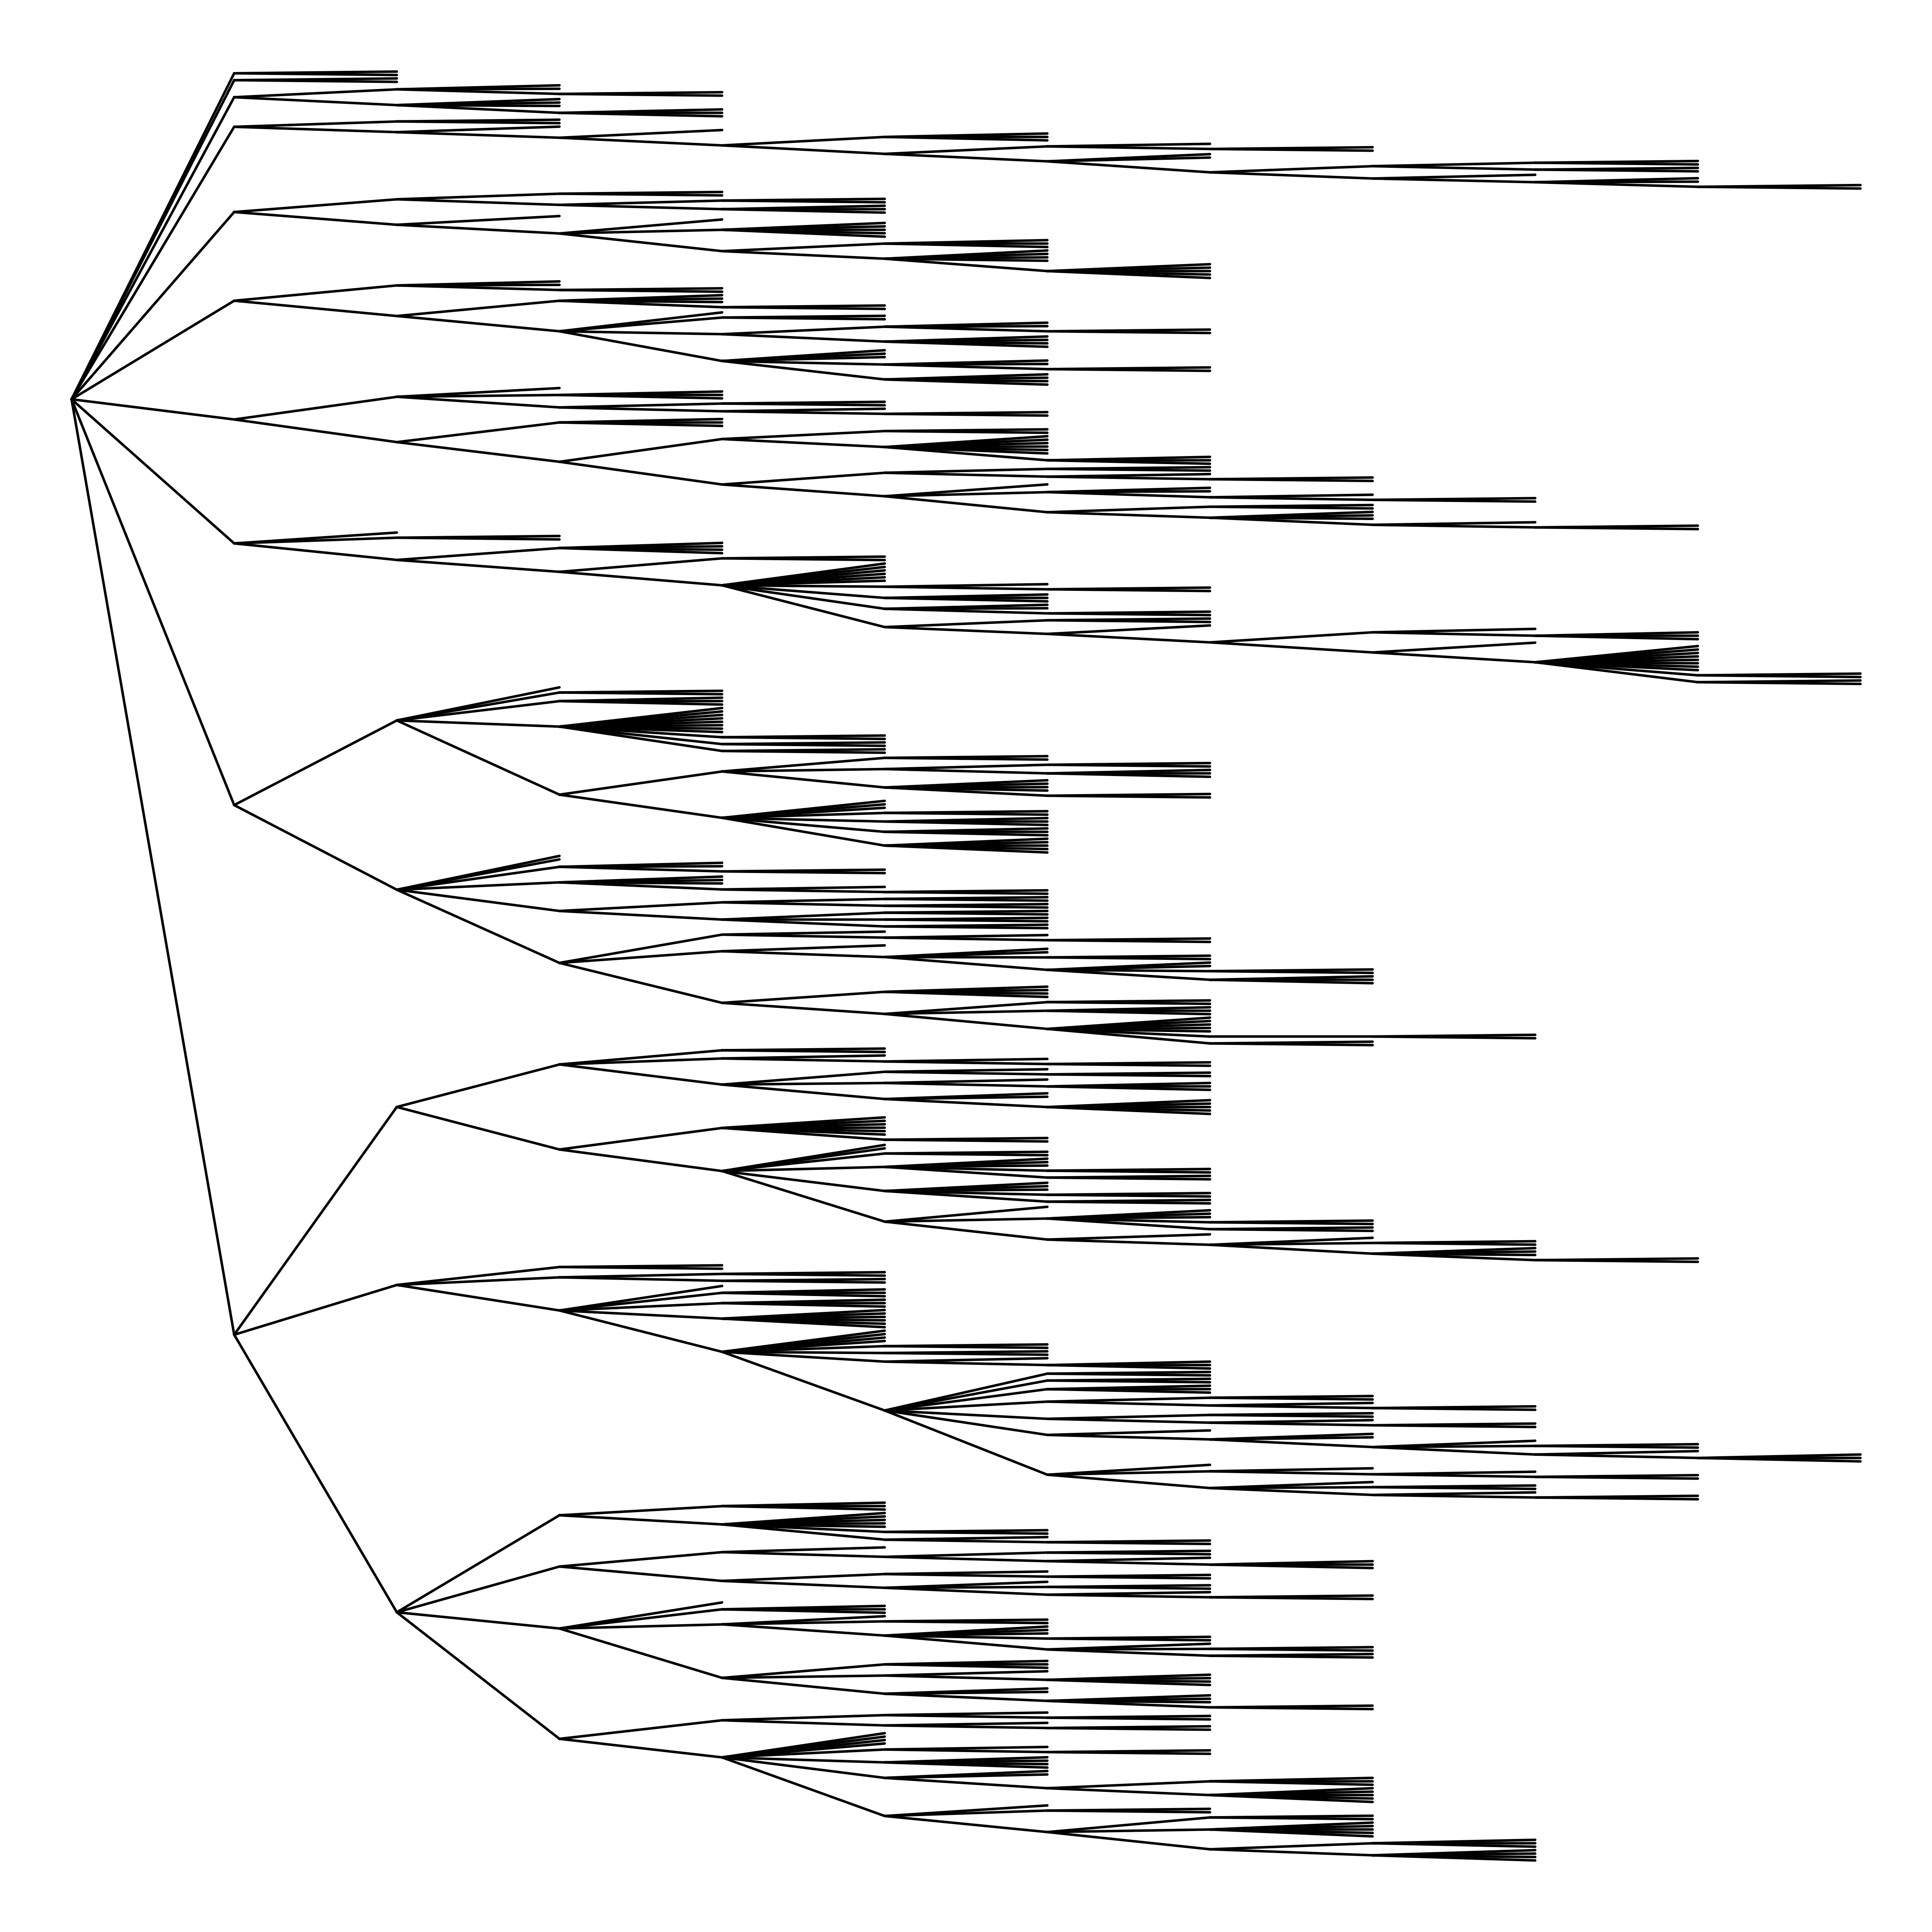
\includegraphics[width=3.5cm]{illustrations/plots_from_R/coverage_plots/tree/Oceanic_glottolog_tree_bare.png} &includes all Oceanic languages & has no branch lengths; possibly inconsistent sub-grouping; many polytomies (10\%); lowest proportion of D-estimates similar to 0 \\
\midrule
\citet{grayetal_2009} - MCCT & 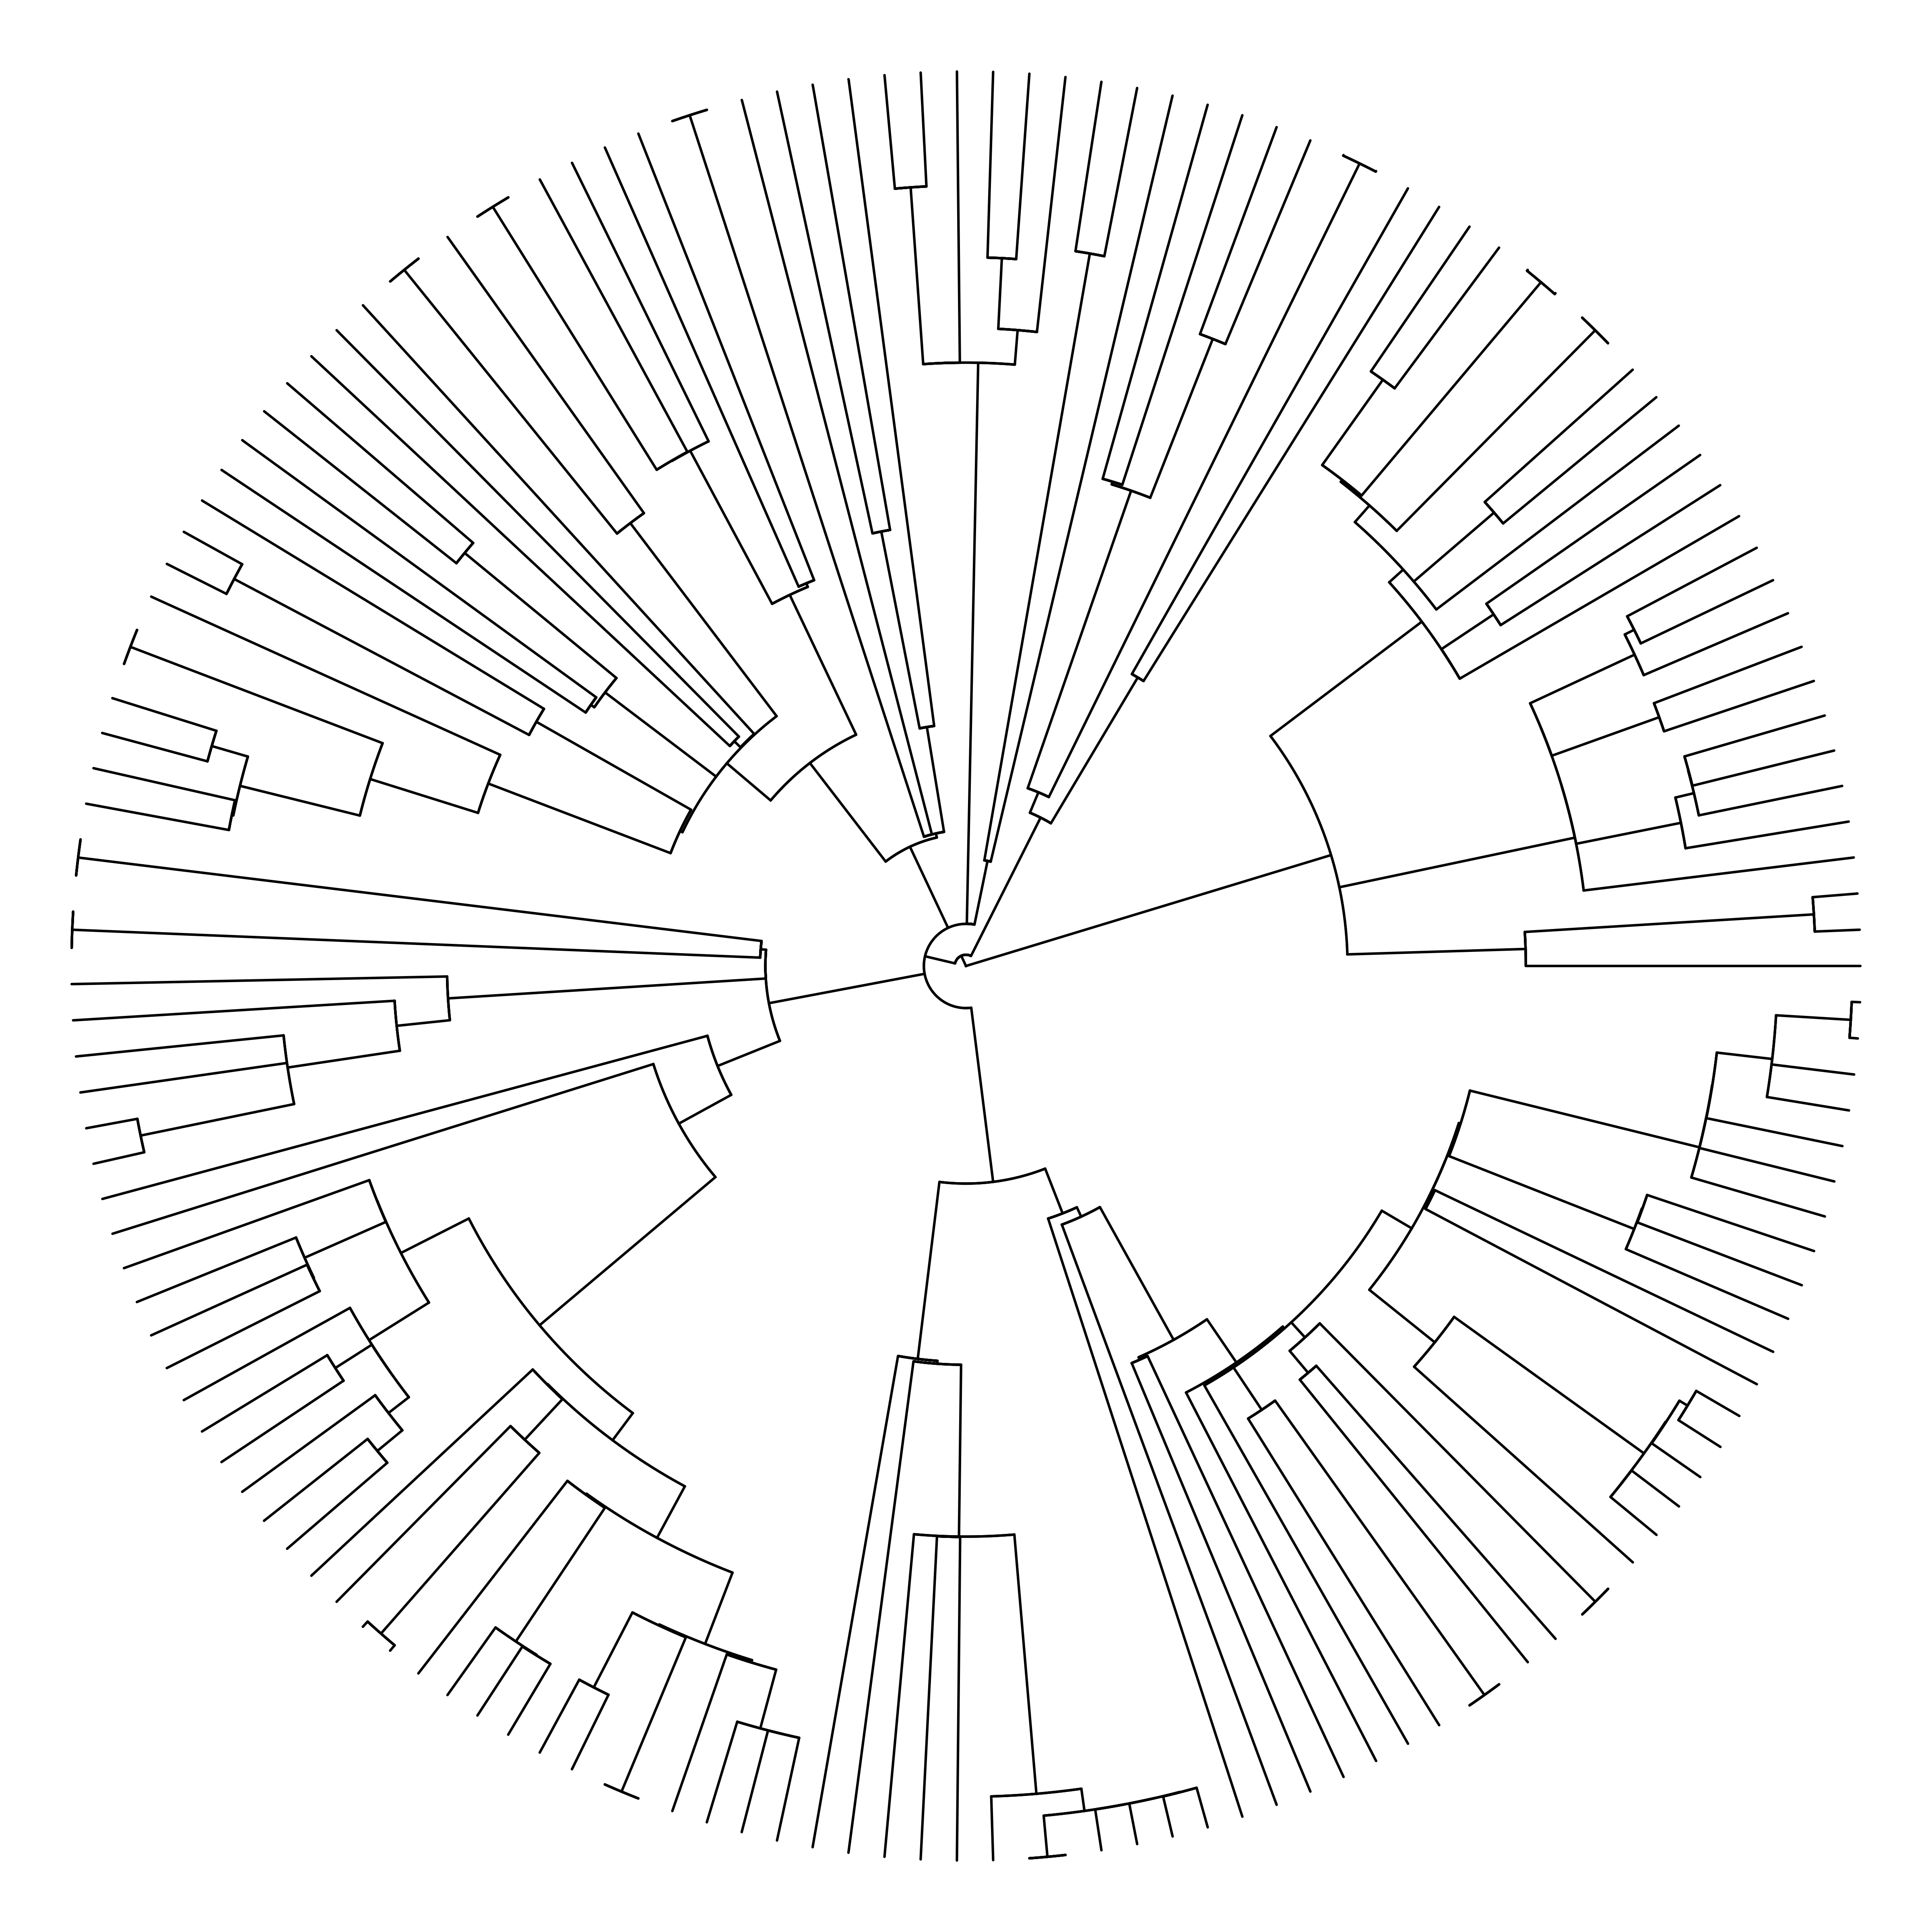
\includegraphics[width=3.5cm]{illustrations/plots_from_R/coverage_plots/tree/Oceanic_gray_et_al_tree_mcct_bare.png} &has branch lengths; is based on explicit lexical data; transparent methodology at each step; fewer polytomies (3\%) & includes fewer languages \\
\midrule
\citet{grayetal_2009} - random sample of 100 from posterior &  \includegraphics[width=3.5cm]{illustrations/plots_from_R/coverage_plots/tree/gray_et_al_2009_100_sample_densitree.png}& has branch lengths; is based on explicit lexical data; transparent methodology at each step; much fewer polytomies (0.15\%); encompasses more variation than MCCT; highest proportion of D-estimates similar to 0 & includes fewer languages; takes longer time to calculate over\\
\bottomrule
\end{tabular}
\end{table}

\FloatBarrier

Once more, given that branch lengths matter if we want to understand the past we ought to go with the trees from \cite{grayetal_2009}. After all, an equal amount of time has passed between the existence of a proto-community to today's extant languages, and we take our trees to estimate that history. It is possible that some languages are more conservative than others in their sounds, words or grammar, but in such cases, we should let the models figure that out rather than set all branches to the same length. When it comes to ancient languages, like Latin, Akkadian etc, it makes sense to place these at a closer distance to the root (as done for example in \citet{carling2021reconstructing}). However, the differences in root-to-tip distances that a tree like Glottolog suggests for Oceanic seem extreme see Fig. \ref{fig:branch_lengths} in Supplementary Material \ref{supp:tree_details}). 

While the MCCT is a practical summary of the 4,200 posterior trees, sampling over the actual set of posterior trees is preferable since it incorporates uncertainly in a better way and involves fewer polytomies.

Conceptually, the most reliable results \emph{a priori} are those derived from Maximum Likelihood + random sample over posterior.

Now to the practical comparison, how does the computational approaches compare to conventional HL? Overall there is a high degree of concordance with reconstructions from expert historical linguists and all approaches. Reconstructions by both Maximum Parsimony and Maximum Likelihood agreed to a very large extent with the findings from historical linguistics. This suggests that the mechanisms at work in historical linguistic reconstruction may be similar to the concepts underlying the computational methods presented in this paper. The agreement was the highest when most of the languages had or lacked a feature (see Supplementary Material \ref{supp:cor_min_p_HL}), but it was generally high also when there was more variability.

The preferable method conceptually, Maximum Likelihood + random sample over \citet{grayetal_2009} posterior, did not have the highest concordance (including half-results) score with HL - 0.87. The variation between the results was not large, however. The method that was the most similar to conventional HL, Parsimony + Glottolog, achieved a concordance of 0.9. The Glottolog-tree contained more matches to Grambank data-points, which is probably why it out-achieved the \cite{grayetal_2009}-trees in concordance with conventional HL.

The methods which do not take into account branch lengths (Maximum Parsimony and Most Common) achieve a somewhat higher concordance with historical linguistics predictions. This is potentially troubling since it seems a sound principle that branch lengths in trees matter.

However, the general concordance between the outcomes of the different methods studied here gives us confidence that computational approaches are not so foreign to historical linguistics as they first may appear. 

The classical historical linguistics toolkit is well-developed in terms of sub-grouping, but for future analysis, it would be beneficial to develop a framework regarding branch estimation as well. Pawley (personal correspondence) notes that most of the sub-grouping done in historical linguistics tends to be at the lower level, which suggests that further work on deeper relationships is also needed in order to improve the overall tree-structure (unless we have cause to believe in more community splitting events in recent time compared to long ago). 

Computational methods need not be in conflict with conventional approaches, they can be complementary. There is certainly room for improvements based on knowledge from classical historical linguistics. When there were disagreements among linguists in regard to the structure of proto-languages, we saw more clearly the impact of the lack of information on the plausibility of changes and combinations, as well as contact-induced change. Currently, it is not possible to include information on these parameters directly into the computational ASR-models, because it has not been formalised in such a way that it can be included. If more work was dedicated to formalising such knowledge this may be possible in future. For example, it is possible to supply Maximum Likelihood ASR with a rates matrix that represents the plausibility of changes from one state to another \citep[8-9]{R-corHMM}. It is also possible in other computational approaches to fix certain node states and study what the implications are.

%These results can be interpreted to mean that we have reasons to trust in the results of computational approaches to ASR in linguistics. 

%This means that we have support for using conclusions regarding rate of change etc from the computational methods to estimate knowledge of historical linguists. This can aid us in making the implicit explicit. Whether or not the predictions from classical historical linguistics are correct or not is a different matter, which should be investigated by assessing the soundness of the principles at play and comparing with other evidence.


%but the estimation of branch lengths has received less attention. It is not necessary to ``do dates'' (c.f. \citet[371]{greenhill2015evolution}) precisely to make improvements here, relative chronology that is not tied to specific dates is also 

%\cite{mcmahon_2006}
%This need not mean a return to glottochonology, this appears to be a misguided and overly simplistic approach , there are other alternatives.

The future of research on the history of languages probably lies in the combination of human and computational labour. Curating lexical cognate data \citep{list2022lexibank} and constructing trees \citep{grayetal_2009} still rely on teams of expert linguists annotating word-lists for cognacy. Methods are being developed for automatic cognate detection (c.f. \citet{list2017potential}), but they are not yet ready to replace the vast human knowledge and experience of the experts in historical linguistics. However, once cognate classes, regular sound correspondences and structural features are identified, the work then turns to reconstructing history (sub-grouping or constructing trees/networks) and ASR (c.f. \ref{fig:HL_tasks}). For these tasks, there are suitable computational methods that can be applied such as those in this paper - and others (c.f. \citet{greenhill2015evolution}; \citet{gray_greenhill_defend_bayes} and \citet{joy2016ancestral}). Research into linguistic history can be greatly improved and effectivized by computational tools, which in turn can be given sensible priors and parameters to produce more reliable results in a future joint venture between classical and novel methods.

In order to improve these methods, we should attempt to include the knowledge that historical linguists have about plausibility of changes, harmonics of traits and contact events. Scholars of Oceanic languages have also acquired an immense knowledge of the languages, cultures and societies of the Pacific. This is why their research is so valuable and trusted. Some or all of this kind of information can be incorporated to guide computational methods, for example as priors in models. These priors should not be given the power to entirely constrain the outcomes, but guide the conclusions the method reaches given the data. In order for this to happen, more information needs to be made explicit in historical linguistics studies.

It is no doubt difficult to convey this wealth of contextual information in each and every academic paper. The task becomes further complex when we need to aggregate the knowledge and make it comparable and consistent across publications. Nevertheless, this is where I believe that the path of scientific discovery leads us next - computers and humans together.

Conversely, it is also desirable that computational methodologies and phylogenetics are made more accessible to the wider linguistics community and incorporated into historical linguistics education. It is my perception that there is at times a disconnect between newer and classical approaches in this space, which is unnecessary and detrimental. It is my hope that this paper has made some advancements in both introducing historical linguists to some concepts in computational approaches to ASR and introducing non-linguists to ASR in historical linguistics more generally.

The more methodology and analytical choices are made explicit, the easier it is to assess the soundness of the study, replicate it and improve upon it. There are areas of this study that I look forward to receiving feedback on so that we can advance together as a field. This study aims at increasing the transparency of both the principles of reconstruction in classical historical linguistics and the corresponding computational approaches. Hopefully, this study (alongside \citet{carling2021reconstructing} and \citet{goldstein_2022}) can be a starting point for more joint ventures into our cultural past.




%In addition, we also need to encourage co-operation between traditional historical linguists and linguists applying new methods, as exemplified in this paper, when it comes to estimating branch lengths. Many trees proposed in classical studies of historical linguistics do not necessarily 

%One of the key pieces of information that is missing from this analysis is plausibility of changes and combinations of features.

%Within Oceanic historical linguistics, there exists a debate regarding the nature of the alignment system of Proto-Polynesian. The results of this study support the analysis that it was ergative. However, since the computational reconstructions are unable to take into account considerations of plausibility, which is the main difference between the different proposals, this cannot be taken as hard evidence. Further work in this area should seek to incorporate information about plausibility in order to increase the reliability of this result.m

%explicit information on plausibility of rate of change and combinations of traits
%ways of estimating contact events
%models of history (trees/networks) with meaningful branch/edge lengths
%more training of computational methods to historical linguistics students
%more carefully coded data from HL to input to reasonable computational models


\bibliographystyle{unified}
\bibliography{ASR_Oceanic, bib_from_r/used_pkgs}

\FloatBarrier

%\section*{Funding information}
%Grant or other funding acknowledgements should go here.

\newpage
\section*{Acknowledgements}
I am fortunate enough to have colleagues in academia who have been generous and helped me with technical matters and working through methodology conceptually, these are: Stephen Mann, Angela Chira, Jordan Brock, 華夏 Xià Huá, Cara Evans, Benedict King, Gerd Carling, Chundra Cathcart, Cristian Juárez, Viktor Martinović, Robert Tegethoff, Natalia Chousou-Polydouri, Sandra Auderset, Russell Gray and Hannah Haynie. Mary Walworth has been very helpful in reviewing the Grambank coding of Oceanic proto-languages. I am also grateful to the two anonymous reviewers at Diachronica for their valuable feedback and to my former PhD supervisors Andrew Pawley, Nicholas Evans, Mark Ellison and Simon Greenhill who also provided valuable commentary. Any mistakes and misconceptions that remain are my own.

%\section*{Abbreviations}
%A list of abbreviations used in the text should appear here.

\newpage

\appendix
\section*{Appendices}
\addcontentsline{toc}{section}{Appendices}
\renewcommand{\thesubsection}{\Alph{subsection}}

\subsection{Data and code availability}
\label{supp_data_availability}
This study involves data from Grambank (v1.0, \cite{grambank_dataset_zenodo_v1, grambank_release}, D-PLACE (v2.2.1 \citet{d_place_all} and Glottolog (v4.5, \citet{glottolog4_5}. The study also involves the use of some scripts associated with the release of Grambank v1.0 which are found in the repository `grambank-analysed` (v1.0, \citet{grambank_analysed_1_0}). Inside of the `grambank-analysed` project lies Glottolog and Grambank. The trees from \citet{grayetal_2009} are stored in the D-PLACE repository, the Glottolog tree in the glottolog-cldf repository.

All the R-scripts for data wrangling, analysis and plotting are found on GitHub and Zenodo.

Zenodo locations:

\begin{itemize}
\item Oceanic\_computational\_ASR  \textcolor{red}{TBA Zenodo-url}
\item Grambank-analysed (v1.0) \url{https://doi.org/10.5281/zenodo.7740822}
\begin{itemize}
\item Grambank (v.1.0) \url{https://doi.org/10.5281/zenodo.7740140}
\item glottolog-cldf (v4.5) \url{https://doi.org/10.5281/zenodo.5772642}
\end{itemize}
\item dplace-data (v2.2.1) \url{https://doi.org/10.5281/zenodo.5554395}
\end{itemize}

GitHub locations:
\begin{itemize}
\item Oceanic\_computational\_ASR \url{https://github.com/HedvigS/Oceanic_computational_ASR}
\item Grambank-analysed (v1.0) \url{https://github.com/grambank/grambank-analysed/tree/v1.0} --- which in turn contains submodules of:
\begin{itemize}
\item Grambank (v1.0) \url{https://github.com/grambank/grambank/tree/v1.0}
\item glottolog-cldf (v4.5) \url{https://github.com/glottolog/glottolog-cldf/tree/v4.5}
\end{itemize}
\item dplace-data (v2.2.1) \url{https://github.com/D-PLACE/dplace-data/tree/v2.2.1}
\end{itemize}



\subsection{Grambank features}
\label{Grambank_features}
Table \ref{GB_features_table} contains Grambank features which serves as the input to the analysis. Multistate features have been binarised. For more details, see appendix \ref{supp:dataset_details}, \citet{grambank_release}: Materials and methods: Data and the parameters-table in the CLDF-release on Zenodo of the grambank dataset version 1 \citep{grambank_dataset_zenodo_v1}. Documentation of the features, including procedures and examples are also found on a GitHub wiki  \url{https://github.com/grambank/grambank/wiki} that is updated continuously. Release-versions are published regularly, as data-sets on Zenodo.



%\begin{landscape}
% latex table generated in R 4.3.0 by xtable 1.8-4 package
% Sat Jun 10 22:23:05 2023
\begin{longtable}{p{3cm}p{12cm}}
  \toprule
Feature_ID & Name \\ 
  \midrule
GB024a & Is the order of the numeral and noun Num-N? \\ 
  GB024b & Is the order of the numeral and noun N-Num? \\ 
  GB025a & Is the order of the adnominal demonstrative and noun Dem-N? \\ 
  GB025b & Is the order of the adnominal demonstrative and noun N-Dem? \\ 
  GB065a & Is the pragmatically unmarked order of adnominal possessor noun and possessed noun PSR-PSD? \\ 
  GB065b & Is the pragmatically unmarked order of adnominal possessor noun and possessed noun PSD-PSR? \\ 
  GB130a & Is the pragmatically unmarked order of S and V in intransitive clauses S-V? \\ 
  GB130b & Is the pragmatically unmarked order of S and V in intransitive clauses V-S? \\ 
  GB193a & Is the order of the adnominal property word (ANM) and noun ANM-N? \\ 
  GB193b & Is the order of the adnominal property word (ANM) and noun N-ANM? \\ 
  GB203a & Is the order of the adnominal collective universal quantifier (UQ) and noun UQ-N? \\ 
  GB203b & Is the order of the adnominal collective universal quantifier (UQ) and noun N-QU? \\ 
  GB020 & Are there definite or specific articles? \\ 
  GB021 & Do indefinite nominals commonly have indefinite articles? \\ 
  GB022 & Are there prenominal articles? \\ 
  GB023 & Are there postnominal articles? \\ 
  GB026 & Can adnominal property words occur discontinuously? \\ 
  GB027 & Are nominal conjunction and comitative expressed by different elements? \\ 
  GB028 & Is there a distinction between inclusive and exclusive? \\ 
  GB030 & Is there a gender distinction in independent 3rd person pronouns? \\ 
  GB031 & Is there a dual or unit augmented form (in addition to plural or augmented) for all person categories in the pronoun system? \\ 
  GB035 & Are there three or more distance contrasts in demonstratives? \\ 
  GB036 & Do demonstratives show an elevation distinction? \\ 
  GB037 & Do demonstratives show a visible-nonvisible distinction? \\ 
  GB038 & Are there demonstrative classifiers? \\ 
  GB039 & Is there nonphonological allomorphy of noun number markers? \\ 
  GB041 & Are there several nouns (more than three) which are suppletive for number? \\ 
  GB042 & Is there productive overt morphological singular marking on nouns? \\ 
  GB043 & Is there productive morphological dual marking on nouns? \\ 
  GB044 & Is there productive morphological plural marking on nouns? \\ 
  GB046 & Is there an associative plural marker for nouns? \\ 
  GB047 & Is there a productive morphological pattern for deriving an action/state noun from a verb? \\ 
  GB048 & Is there a productive morphological pattern for deriving an agent noun from a verb? \\ 
  GB049 & Is there a productive morphological pattern for deriving an object noun from a verb? \\ 
  GB051 & Is there a gender/noun class system where sex is a factor in class assignment? \\ 
  GB052 & Is there a gender/noun class system where shape is a factor in class assignment? \\ 
  GB053 & Is there a gender/noun class system where animacy is a factor in class assignment? \\ 
  GB054 & Is there a gender/noun class system where plant status is a factor in class assignment? \\ 
  GB057 & Are there numeral classifiers? \\ 
  GB058 & Are there possessive classifiers? \\ 
  GB059 & Is the adnominal possessive construction different for alienable and inalienable nouns? \\ 
  GB068 & Do core adjectives (defined semantically as property concepts such as value, shape, age, dimension) act like verbs in predicative position? \\ 
  GB069 & Do core adjectives (defined semantically as property concepts; value, shape, age, dimension) used attributively require the same morphological treatment as verbs? \\ 
  GB070 & Are there morphological cases for non-pronominal core arguments (i.e. S/A/P)? \\ 
  GB071 & Are there morphological cases for pronominal core arguments (i.e. S/A/P)? \\ 
  GB072 & Are there morphological cases for oblique non-pronominal NPs (i.e. not S/A/P)? \\ 
  GB073 & Are there morphological cases for independent oblique personal pronominal arguments (i.e. not S/A/P)? \\ 
  GB074 & Are there prepositions? \\ 
  GB075 & Are there postpositions? \\ 
  GB079 & Do verbs have prefixes/proclitics, other than those that only mark A, S or P (do include portmanteau: A \& S + TAM)? \\ 
  GB080 & Do verbs have suffixes/enclitics, other than those that only mark A, S or P (do include portmanteau: A \& S + TAM)? \\ 
  GB081 & Is there productive infixation in verbs? \\ 
  GB082 & Is there overt morphological marking of present tense on verbs? \\ 
  GB083 & Is there overt morphological marking on the verb dedicated to past tense? \\ 
  GB084 & Is there overt morphological marking on the verb dedicated to future tense? \\ 
  GB086 & Is a morphological distinction between perfective and imperfective aspect available on verbs? \\ 
  GB089 & Can the S argument be indexed by a suffix/enclitic on the verb in the simple main clause? \\ 
  GB090 & Can the S argument be indexed by a prefix/proclitic on the verb in the simple main clause? \\ 
  GB091 & Can the A argument be indexed by a suffix/enclitic on the verb in the simple main clause? \\ 
  GB092 & Can the A argument be indexed by a prefix/proclitic on the verb in the simple main clause? \\ 
  GB093 & Can the P argument be indexed by a suffix/enclitic on the verb in the simple main clause? \\ 
  GB094 & Can the P argument be indexed by a prefix/proclitic on the verb in the simple main clause? \\ 
  GB095 & Are variations in marking strategies of core participants based on TAM distinctions? \\ 
  GB096 & Are variations in marking strategies of core participants based on verb classes? \\ 
  GB098 & Are variations in marking strategies of core participants based on person distinctions? \\ 
  GB099 & Can verb stems alter according to the person of a core participant? \\ 
  GB103 & Is there a benefactive applicative marker on the verb (including indexing)? \\ 
  GB104 & Is there an instrumental applicative marker on the verb (including indexing)? \\ 
  GB105 & Can the recipient in a ditransitive construction be marked like the monotransitive patient? \\ 
  GB107 & Can standard negation be marked by an affix, clitic or modification of the verb? \\ 
  GB108 & Is there directional or locative morphological marking on verbs? \\ 
  GB109 & Is there verb suppletion for participant number? \\ 
  GB110 & Is there verb suppletion for tense or aspect? \\ 
  GB111 & Are there conjugation classes? \\ 
  GB113 & Are there verbal affixes or clitics that turn intransitive verbs into transitive ones? \\ 
  GB114 & Is there a phonologically bound reflexive marker on the verb? \\ 
  GB115 & Is there a phonologically bound reciprocal marker on the verb? \\ 
  GB116 & Do verbs classify the shape, size or consistency of absolutive arguments by means of incorporated nouns, verbal affixes or suppletive verb stems? \\ 
  GB117 & Is there a copula for predicate nominals? \\ 
  GB118 & Are there serial verb constructions? \\ 
  GB119 & Can mood be marked by an inflecting word (""""""""auxiliary verb"""""""")? \\ 
  GB120 & Can aspect be marked by an inflecting word (""""""""auxiliary verb"""""""")? \\ 
  GB121 & Can tense be marked by an inflecting word (""""""""auxiliary verb"""""""")? \\ 
  GB122 & Is verb compounding a regular process? \\ 
  GB123 & Are there verb-adjunct (aka light-verb) constructions? \\ 
  GB124 & Is incorporation of nouns into verbs a productive intransitivizing process? \\ 
  GB126 & Is there an existential verb? \\ 
  GB127 & Are different posture verbs used obligatorily depending on an inanimate locatum's shape or position (e.g. 'to lie' vs. 'to stand')? \\ 
  GB129 & Is there a notably small number, i.e. about 100 or less, of verb roots in the language? \\ 
  GB131 & Is a pragmatically unmarked constituent order verb-initial for transitive clauses? \\ 
  GB132 & Is a pragmatically unmarked constituent order verb-medial for transitive clauses? \\ 
  GB133 & Is a pragmatically unmarked constituent order verb-final for transitive clauses? \\ 
  GB134 & Is the order of constituents the same in main and subordinate clauses? \\ 
  GB135 & Do clausal objects usually occur in the same position as nominal objects? \\ 
  GB136 & Is the order of core argument (i.e. S/A/P) constituents fixed? \\ 
  GB137 & Can standard negation be marked clause-finally? \\ 
  GB138 & Can standard negation be marked clause-initially? \\ 
  GB139 & Is there a difference between imperative (prohibitive) and declarative negation constructions? \\ 
  GB140 & Is verbal predication marked by the same negator as all of the following types of predication: locational, existential and nominal? \\ 
  GB146 & Is there a morpho-syntactic distinction between predicates expressing controlled versus uncontrolled events or states? \\ 
  GB147 & Is there a morphological passive marked on the lexical verb? \\ 
  GB148 & Is there a morphological antipassive marked on the lexical verb? \\ 
  GB149 & Is there a morphologically marked inverse on verbs? \\ 
  GB150 & Is there clause chaining? \\ 
  GB151 & Is there an overt verb marker dedicated to signalling coreference or noncoreference between the subject of one clause and an argument of an adjacent clause (""""""""switch reference"""""""")? \\ 
  GB152 & Is there a morphologically marked distinction between simultaneous and sequential clauses? \\ 
  GB155 & Are causatives formed by affixes or clitics on verbs? \\ 
  GB156 & Is there a causative construction involving an element that is unmistakably grammaticalized from a verb for 'to say'? \\ 
  GB158 & Are verbs reduplicated? \\ 
  GB159 & Are nouns reduplicated? \\ 
  GB160 & Are elements apart from verbs or nouns reduplicated? \\ 
  GB165 & Is there productive morphological trial marking on nouns? \\ 
  GB166 & Is there productive morphological paucal marking on nouns? \\ 
  GB167 & Is there a logophoric pronoun? \\ 
  GB170 & Can an adnominal property word agree with the noun in gender/noun class? \\ 
  GB171 & Can an adnominal demonstrative agree with the noun in gender/noun class? \\ 
  GB172 & Can an article agree with the noun in gender/noun class? \\ 
  GB177 & Can the verb carry a marker of animacy of argument, unrelated to any gender/noun class of the argument visible in the NP domain? \\ 
  GB184 & Can an adnominal property word agree with the noun in number? \\ 
  GB185 & Can an adnominal demonstrative agree with the noun in number? \\ 
  GB186 & Can an article agree with the noun in number? \\ 
  GB187 & Is there any productive diminutive marking on the noun (exclude marking by system of nominal classification only)? \\ 
  GB188 & Is there any productive augmentative marking on the noun (exclude marking by system of nominal classification only)? \\ 
  GB192 & Is there a gender system where a noun's phonological properties are a factor in class assignment? \\ 
  GB196 & Is there a male/female distinction in 2nd person independent pronouns? \\ 
  GB197 & Is there a male/female distinction in 1st person independent pronouns? \\ 
  GB198 & Can an adnominal numeral agree with the noun in gender/noun class? \\ 
  GB204 & Do collective ('all') and distributive ('every') universal quantifiers differ in their forms or their syntactic positions? \\ 
  GB250 & Can predicative possession be expressed with a transitive 'habeo' verb? \\ 
  GB252 & Can predicative possession be expressed with an S-like possessum and a locative-coded possessor? \\ 
  GB253 & Can predicative possession be expressed with an S-like possessum and a dative-coded possessor? \\ 
  GB254 & Can predicative possession be expressed with an S-like possessum and a possessor that is coded like an adnominal possessor? \\ 
  GB256 & Can predicative possession be expressed with an S-like possessor and a possessum that is coded like a comitative argument? \\ 
  GB257 & Can polar interrogation be marked by intonation only? \\ 
  GB260 & Can polar interrogation be indicated by a special word order? \\ 
  GB262 & Is there a clause-initial polar interrogative particle? \\ 
  GB263 & Is there a clause-final polar interrogative particle? \\ 
  GB264 & Is there a polar interrogative particle that most commonly occurs neither clause-initially nor clause-finally? \\ 
  GB265 & Is there a comparative construction that includes a form that elsewhere means 'surpass, exceed'? \\ 
  GB266 & Is there a comparative construction that employs a marker of the standard which elsewhere has a locational meaning? \\ 
  GB270 & Can comparatives be expressed using two conjoined clauses? \\ 
  GB273 & Is there a comparative construction with a standard marker that elsewhere has neither a locational meaning nor a 'surpass/exceed' meaning? \\ 
  GB275 & Is there a bound comparative degree marker on the property word in a comparative construction? \\ 
  GB276 & Is there a non-bound comparative degree marker modifying the property word in a comparative construction? \\ 
  GB285 & Can polar interrogation be marked by a question particle and verbal morphology? \\ 
  GB286 & Can polar interrogation be indicated by overt verbal morphology only? \\ 
  GB291 & Can polar interrogation be marked by tone? \\ 
  GB296 & Is there a phonologically or morphosyntactically definable class of ideophones that includes ideophones depicting imagery beyond sound? \\ 
  GB297 & Can polar interrogation be indicated by a V-not-V construction? \\ 
  GB298 & Can standard negation be marked by an inflecting word (""""""""auxiliary verb"""""""")? \\ 
  GB299 & Can standard negation be marked by a non-inflecting word (""""""""auxiliary particle"""""""")? \\ 
  GB300 & Does the verb for 'give' have suppletive verb forms? \\ 
  GB301 & Is there an inclusory construction? \\ 
  GB302 & Is there a phonologically free passive marker (""""""""particle"""""""" or """"""""auxiliary"""""""")? \\ 
  GB303 & Is there a phonologically free antipassive marker (""""""""particle"""""""" or """"""""auxiliary"""""""")? \\ 
  GB304 & Can the agent be expressed overtly in a passive clause? \\ 
  GB305 & Is there a phonologically independent reflexive pronoun? \\ 
  GB306 & Is there a phonologically independent non-bipartite reciprocal pronoun? \\ 
  GB309 & Are there multiple past or multiple future tenses, distinguishing distance from Time of Reference? \\ 
  GB312 & Is there overt morphological marking on the verb dedicated to mood? \\ 
  GB313 & Are there special adnominal possessive pronouns that are not formed by an otherwise regular process? \\ 
  GB314 & Can augmentative meaning be expressed productively by a shift of gender/noun class? \\ 
  GB315 & Can diminutive meaning be expressed productively by a shift of gender/noun class? \\ 
  GB316 & Is singular number regularly marked in the noun phrase by a dedicated phonologically free element? \\ 
  GB317 & Is dual number regularly marked in the noun phrase by a dedicated phonologically free element? \\ 
  GB318 & Is plural number regularly marked in the noun phrase by a dedicated phonologically free element? \\ 
  GB319 & Is trial number regularly marked in the noun phrase by a dedicated phonologically free element? \\ 
  GB320 & Is paucal number regularly marked in the noun phrase by a dedicated phonologically free element? \\ 
  GB321 & Is there a large class of nouns whose gender/noun class is not phonologically or semantically predictable? \\ 
  GB322 & Is there grammatical marking of direct evidence (perceived with the senses)? \\ 
  GB323 & Is there grammatical marking of indirect evidence (hearsay, inference, etc.)? \\ 
  GB324 & Is there an interrogative verb for content interrogatives (who?, what?, etc.)? \\ 
  GB325 & Is there a count/mass distinction in interrogative quantifiers? \\ 
  GB326 & Do (nominal) content interrogatives normally or frequently occur in situ? \\ 
  GB327 & Can the relative clause follow the noun? \\ 
  GB328 & Can the relative clause precede the noun? \\ 
  GB329 & Are there internally-headed relative clauses? \\ 
  GB330 & Are there correlative relative clauses? \\ 
  GB331 & Are there non-adjacent relative clauses? \\ 
  GB333 & Is there a decimal numeral system? \\ 
  GB334 & Is there synchronic evidence for any element of a quinary numeral system? \\ 
  GB335 & Is there synchronic evidence for any element of a vigesimal numeral system? \\ 
  GB336 & Is there a body-part tallying system? \\ 
  GB400 & Are all person categories neutralized in some voice, tense, aspect, mood and/or negation? \\ 
  GB401 & Is there a class of patient-labile verbs? \\ 
  GB402 & Does the verb for 'see' have suppletive verb forms? \\ 
  GB403 & Does the verb for 'come' have suppletive verb forms? \\ 
  GB408 & Is there any accusative alignment of flagging? \\ 
  GB409 & Is there any ergative alignment of flagging? \\ 
  GB410 & Is there any neutral alignment of flagging? \\ 
  GB415 & Is there a politeness distinction in 2nd person forms? \\ 
  GB421 & Is there a preposed complementizer in complements of verbs of thinking and/or knowing? \\ 
  GB422 & Is there a postposed complementizer in complements of verbs of thinking and/or knowing? \\ 
  GB430 & Can adnominal possession be marked by a prefix on the possessor? \\ 
  GB431 & Can adnominal possession be marked by a prefix on the possessed noun? \\ 
  GB432 & Can adnominal possession be marked by a suffix on the possessor? \\ 
  GB433 & Can adnominal possession be marked by a suffix on the possessed noun? \\ 
  GB519 & Can mood be marked by a non-inflecting word (""""""""auxiliary particle"""""""")? \\ 
  GB520 & Can aspect be marked by a non-inflecting word (""""""""auxiliary particle"""""""")? \\ 
  GB521 & Can tense be marked by a non-inflecting word (""""""""auxiliary particle"""""""")? \\ 
  GB522 & Can the S or A argument be omitted from a pragmatically unmarked clause when the referent is inferrable from context (""""""""pro-drop"""""""" or """"""""null anaphora"""""""")? \\ 
   \bottomrule
\caption{Table of Grambank fetures} 
\label{GB_features_table}
\end{longtable}

%\end{landscape}


\FloatBarrier

\subsection{Binarisation of the Grambank features}
\label{supp:dataset_details}
Most of the feature questions are binary (GB027: Are nominal conjunction and comitative expressed by different elements?) but a few are multi-state (GB024 What is the order of numeral and noun in the NP? 1) Num-N, 2) N-Num, 3) both). For the analysis in this study, the multi-state features have been binarised. This is because the values of the multi-state features are not independent of each other; they all contain the value ``Both''. The value ``Num-N'' (numeral before noun) of GB024 is more similar to ``Both'' than it is to the other alternative ``N-Num''. The relationship between the three values are not equal or independent. The table in \ref{Grambank_features} contains a list of all the features used in this study, including the binarised features. The binarization results in a total of 201 features. 

\FloatBarrier

\subsection{Table of historical linguistics sources surveyed}
\label{supp:proto_lg_coding_table}

\begin{longtable}{|p{3cm}|  p{5cm}| p{4cm} | p{3cm}  | p{3cm} |}
\caption{{Table of historical linguistics publications used in this dissertation for Proto-Oceanic grammar}}
\label{HL_prediction_table_summary} \\
\hline
\textbf{Citation}  & \textbf{Title} & \textbf{Proto-Languages}  & \textbf{Domains} \\ \hline
\endfirsthead

\hline
\textbf{Citation}  & \textbf{Title} & \textbf{Proto-Languages}  & \textbf{Domains} \\ \hline
\endhead


\citet{pawley1970change} & Grammatical reconstruction and change on Polynesia and Fiji & Proto-Central Pacific  &Verbal markers and aspect particles \\ \hline

\citet{pawley1973some} & Some problems in Proto-Oceanic & Proto-Oceanic and Proto-Polynesian  & Possession, noun phrase marking, negation, verbal markers, clusivity, word order  \\ \hline

\citet{clark1973aspects} & Aspects of Proto-Polynesian syntax & Proto-Oceanic and Proto-Polynesian  & Alignment, negation, word order, possession, noun phrase marking, voice \\ \hline

\citet{chung1978}  & Case marking and grammatical relations in Polynesian languages & Proto-Polynesian  & Alignment, word order, voice, noun phrase marking \\ \hline

\citet{crowley1985common}  & Common noun phrase marking in Proto-Oceanic & Proto-Oceanic &  noun phrase marking, clusivity  \\ \hline

\citet{jonsson1998} & Det polynesiska verbmorfemet \emph{-Cia}; om dess funktion i Samoanska & Proto-Polynesian & Verbal marker \\ \hline

\citet{marck2000_encyclo} & Polynesian languages (in Facts About the World's Languages: An encyclopaedia of the world's major languages, past and present)& Proto-Central Pacific and Proto-Polynesian & Word order, verbal markers, possession, clusivity \\ \hline

\citet{evans2003study} & A study of valency-changing devices in Proto Oceanic & Proto-Oceanic & Verbal markers \\ \hline

\citet{ball2007ergativity} & On ergativity and accusativity in Proto-Polynesian and proto-Central Pacific&Proto-Polynesian & Alignment, voice \\ \hline

\citet{kikusawa2001rotuman} & Rotuman and Fijian case-marking strategies and their historical development  & Proto-Oceanic & Possession, pronominal number \\ \hline

\citet{kikusawa2002proto}  & Proto Central Pacific ergativity: Its reconstruction and development in the Fijian, Rotuman and Polynesian languages & Proto-Central Pacific   & Alignment, word order \\ \hline

\citet{lynchrosscrowley_proto_grammar_oceanic} & The Oceanic Languages, paper 4: Proto-Oceanic & Proto-Oceanic, Proto-Central Pacific and Proto-Polynesian & Negation, word order, verbal markers, clusivity, possession, pronominal number, polar interrogation, nominalisations and more \\ \hline

\citet{ross2004morphosyntactic}\footnote{This paper makes statements about ``canonical'' Oceanic languages, which is technically different from \emph{reconstruction} of Proto-Oceanic. However, the author does state that the ``canonic type is probably also a reflection of the morphosyntax of Proto Oceanic'' \citep[492]{ross2004morphosyntactic} and has given personal approval for the paper to be included in this study in this manner.}  & The morphosyntactic typology of Oceanic languages &  Proto-Oceanic and Proto-Polynesian  & alignment, word order, verbal markers, possession, noun phrase marking \\ \hline
\end{longtable}
\FloatBarrier


\subsection{R packages used}
\label{supp:r_packages}
All the analysis for this research project was done in the free and open source programming language R, using a multitude of packages. All code and data for this project are available in supplementary material and the locations listed in Supplementary material section \ref{supp_data_availability}. The scripts have been written so that any user of R can execute them. Please see the bibliography for information on package versions. Below are citations for all used packages.

\input{bib_from_r/citation_keys.txt}.

\FloatBarrier
\subsection{Technical details of ASR by Maximum Parsimony and Likelihood}
\label{supp:tech_details}

For Maximum Parsimony, we are using the function \texttt{asr\_max\_parsimony()} from the R-package \texttt{castor} \citep{louca2017efficient} (which is an instantiation of the method described in \citet{sankoff1975minimal}) for calculating ancestral states and stability of features. This function produces ancestral states for all nodes and reports the number of changes that was minimally required for each feature. 

Ancestral state reconstruction using Maximum Likelihood Estimation involves computing each ancestral state from the tips up to the root taking into account branch lengths and the joint likelihood of states given all nodes in the tree \citep{wilks1938large, fisher1912absolute, pagel1994detecting, cunningham1998reconstructing}. The Maximum Likelihood Estimation function takes a set of observations and computes the parameter distribution that maximises the likelihood given the observed data\footnote{For a gentle introduction to the concept of Maximum Likelihood Estimation, see \citet{jonny_ML}.}. This means that for every split in the tree --- every ancestral node --- the Maximum Likelihood Estimation function computes what is the most likely distribution at that point given the nature of the entire tree. ML can be modified so that it allows for different rates of change. An Equal Rates (ER) model assumes that the chance of transition from state A to state B and from B to A are equal. However, we as linguists are aware that certain features are more likely to be lost than gained so this is not a reasonable assumption. Therefore, we allow the model to estimate different transition rates for going from A to B and from B to A given the data. This is known as ``All Rates are Different'' (ARD).

When estimating ancestral states with ML, it is possible to either a) find the state at each node that maximises the likelihood (integrating over all other states at all nodes, in proportion to their probability) at that particular node (marginal reconstruction), or b) find the set of character states at all nodes that (jointly) maximize the likelihood of the entire tree (joint reconstruction). We are using marginal reconstruction in this study since it is the recommended way to deal with uncertainty in reconstruction \citep{revell_2014}. These two methods often yield similar results, but can differ, see \citet[259-260]{felsenstein2004inferring},  \citet[121-126]{yang2006computational} and \citet[5]{joy2016ancestral} for more details. For our data, a trial run of joint reconstruction did not generate drastically different outcomes.

For this study, the function \texttt{R-corHMM} from the \texttt{R}-package \texttt{corHMM} \citep{R-corHMM} is used for marginal reconstruction of ancestral states and rates of change per feature. %Missing data in Grambank for languages included in the analysis was converted to ambiguous, (i.e ? in Grambank $\rightarrow$ 0\&1 for rayDISC()). 

%For the analysis of conservatism per language, the function \texttt{optim.pml()} from \texttt{Phangorn} \citep{phangorn} was used. This function rescales the branches in accordance with the Maximum Likelihood Estimation of change along them. The process of re-scaling the tree in this manner unroots the tree; instead of having root, branches and tips, it becomes an acyclic graph of tips connected by lines of appropriate length. Unrooted trees can be re-rooted using midpoting rooting, outgroup rooting or other methods\footnote{For a visual introduction to outgroup rooting, see \href{this blogpost}{https://phylobotanist.blogspot.com/2015/01/how-to-root-phylogenetic-tree-outgroup.html} by PhyloBotanist.}. For this study, the trees were re-rooted using Nanggu [nang1262], Ayiwoo [ayiw1239] or Natügu [natu1246] as an outgroup. As with the Maximum Parsimony analysis, the distance from the root to each tip was carried out with \texttt{distTip} and the distances were rescaled to between 0 and 1. 

Languages with missing data were pruned away in all analysis, no hidden state reconstruction of values at tips was performed. The match between Glottolog 4.5 and Grambank is 271, the match between \citet{grayetal_2009} and Grambank is 132. For both MP and ML, languages with missing data were dropped from the trees in the analysis for that feature. If after this pruning less than half of the tips remained, that analysis was not carried out.

For both Maximum Parsimony and Maximum Likelihood it is possible for a structural feature to appear and disappear several times along a lineage. This is different from cognate data where a cognate class cannot re-appear.

\FloatBarrier
\newpage
\subsection{Supplementary Figure: distance Scatterplot Matrix}
Fig. \ref{tree_dist_splom} shows the pairwise distances between the same tips in each of the different trees (in the case of the 100 random posterior trees it's the mean distances) and in addition Gower-distances between the same languages given all Grambank features.

\begin{figure}[!ht]
\centering
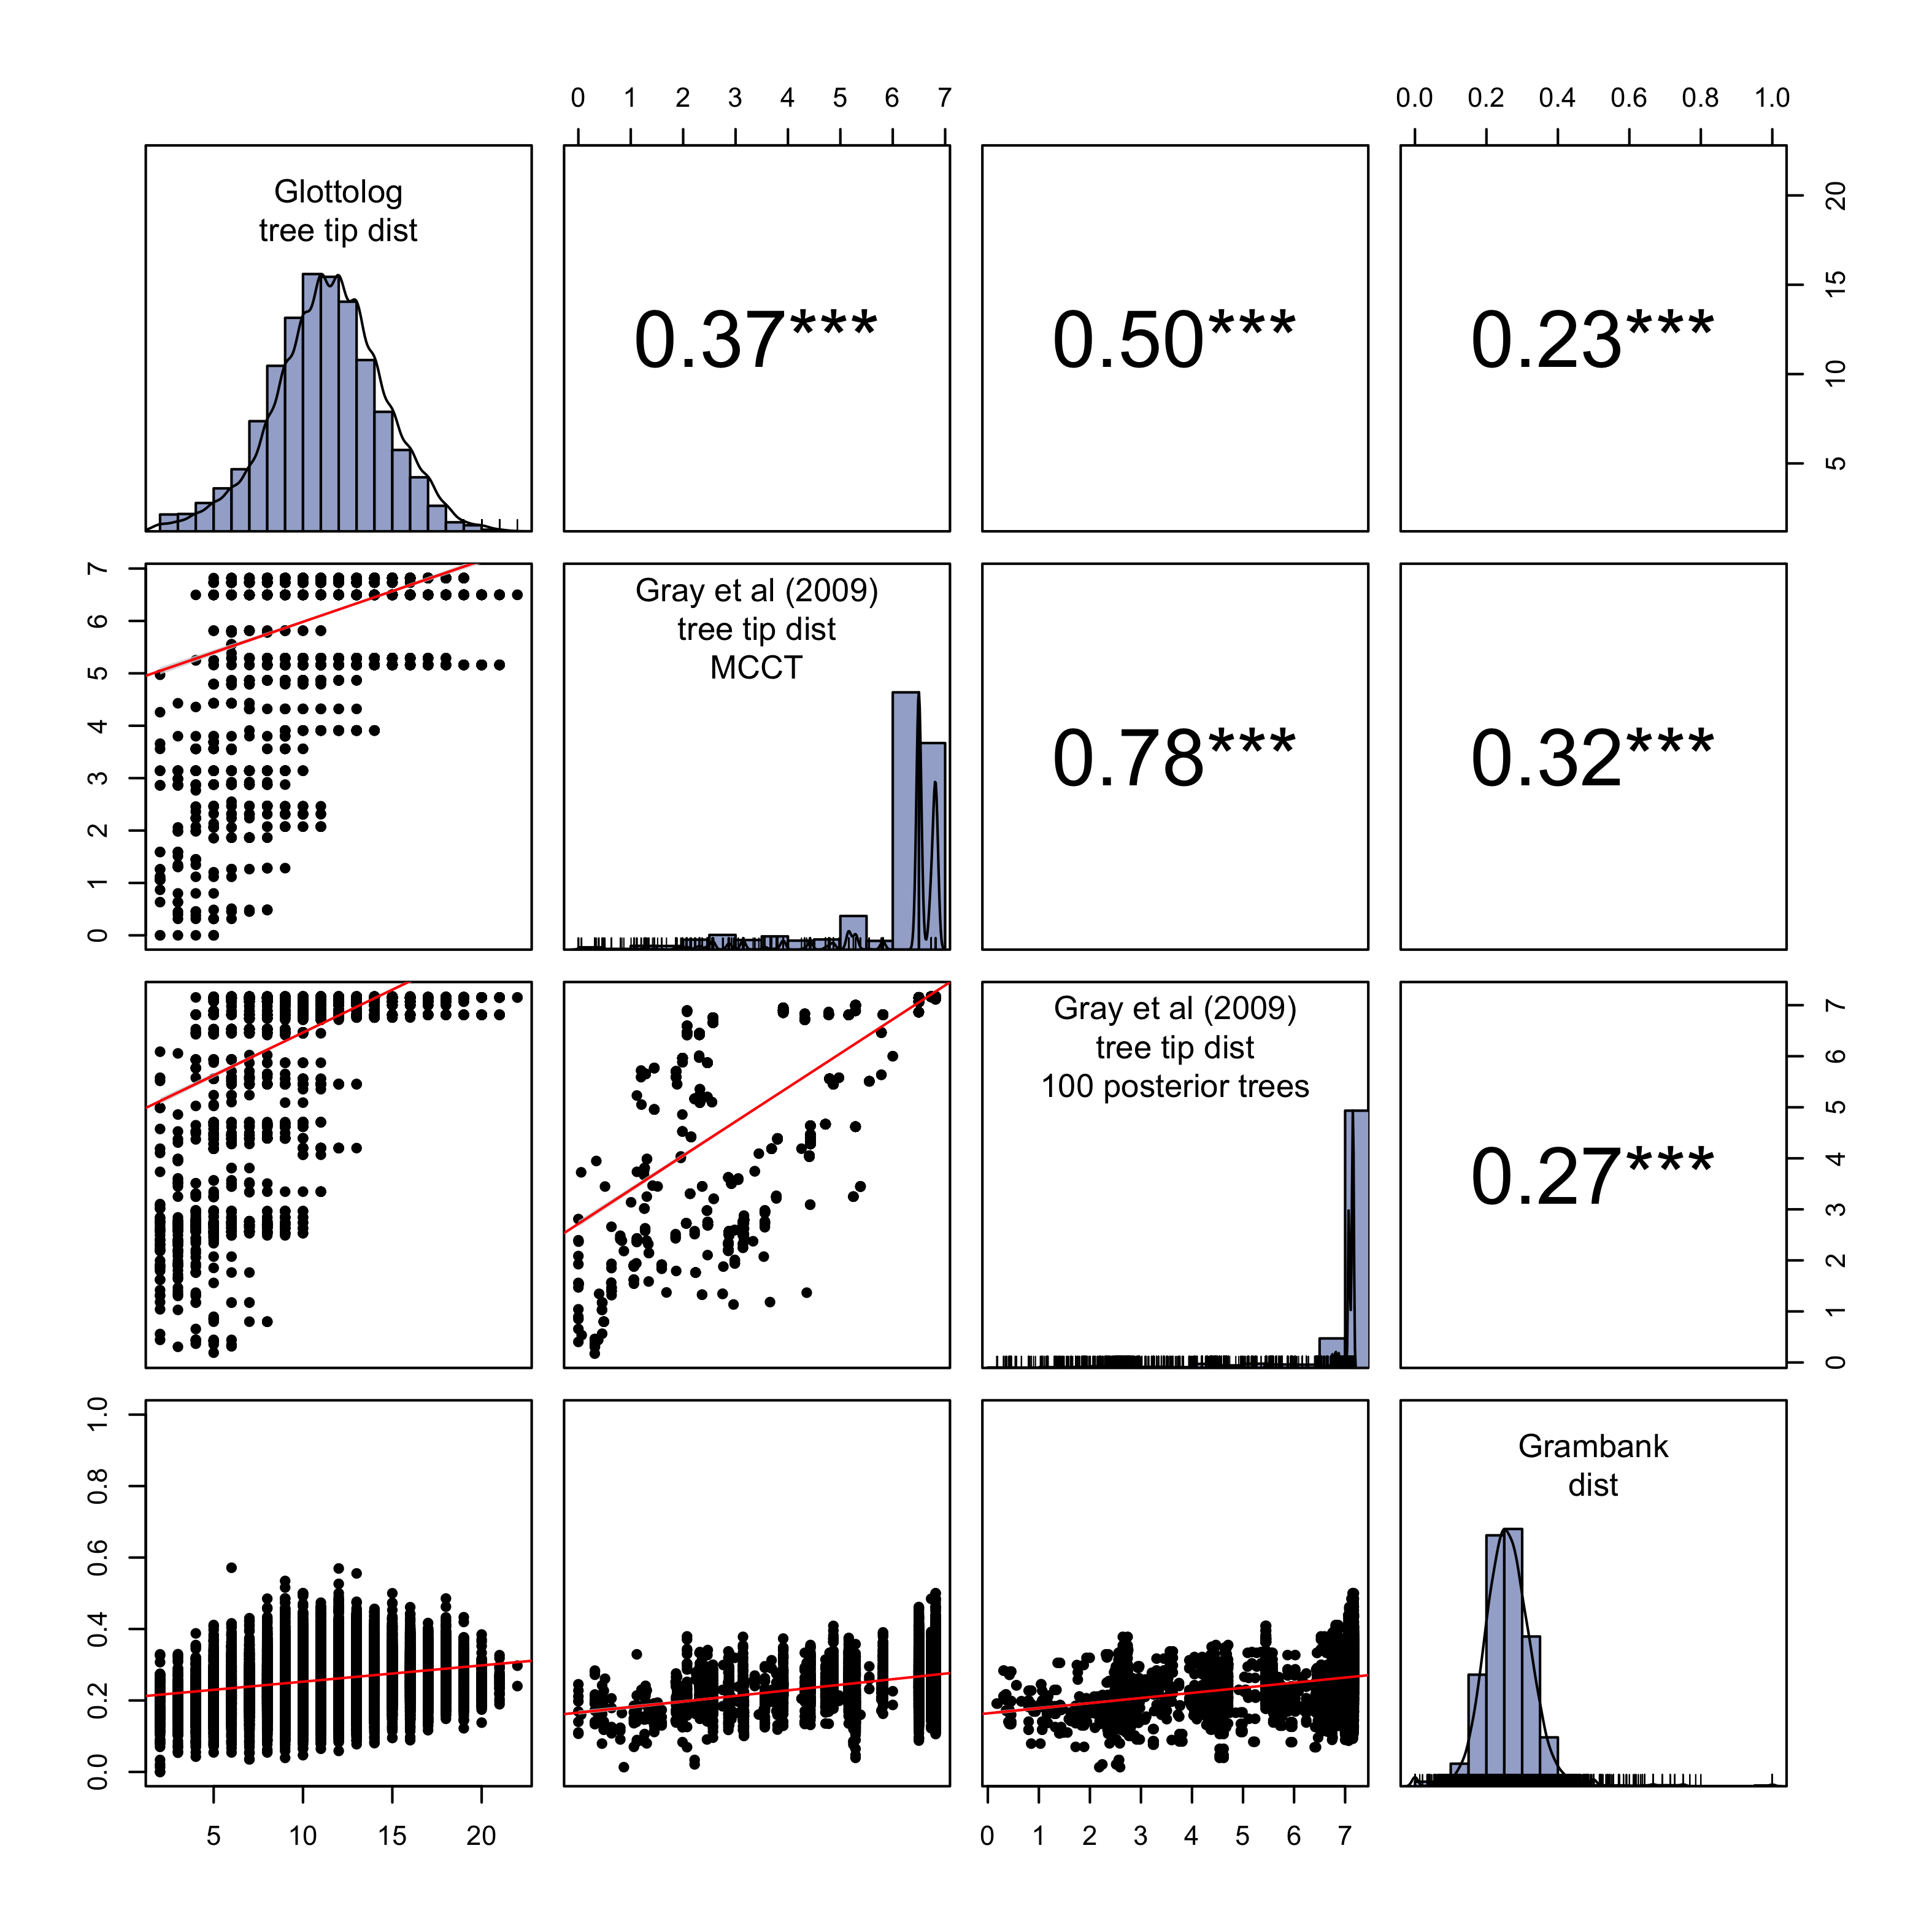
\includegraphics[width=17cm]{illustrations/plots_from_R/SPLOM_tree_dists.png}
\caption{Comparison of distances between tips of the different trees and Grambank. Correlations are Pearson coefficients, the stars indicate the conventional p-value cut-off at 0.05.}
\label{tree_dist_splom}
\end{figure}

\FloatBarrier
\newpage
\subsection{Supplementary Figure: tree heatmap of Gray et al (2009)-MCCT and Grambank variables}
\label{supp:fig_tree_heatmap}

Fig. \ref{fig:tree_heatmap} shows the MCC-tree from \citet{grayetal_2009} and a data-matrix of all 201 binarised Grambank variables. This data is the input for the ASR-analysis for this particular tree and the D-estimate calculation. Missing data is ignored in both sets of analysis.

\begin{figure}[!ht]
\centering
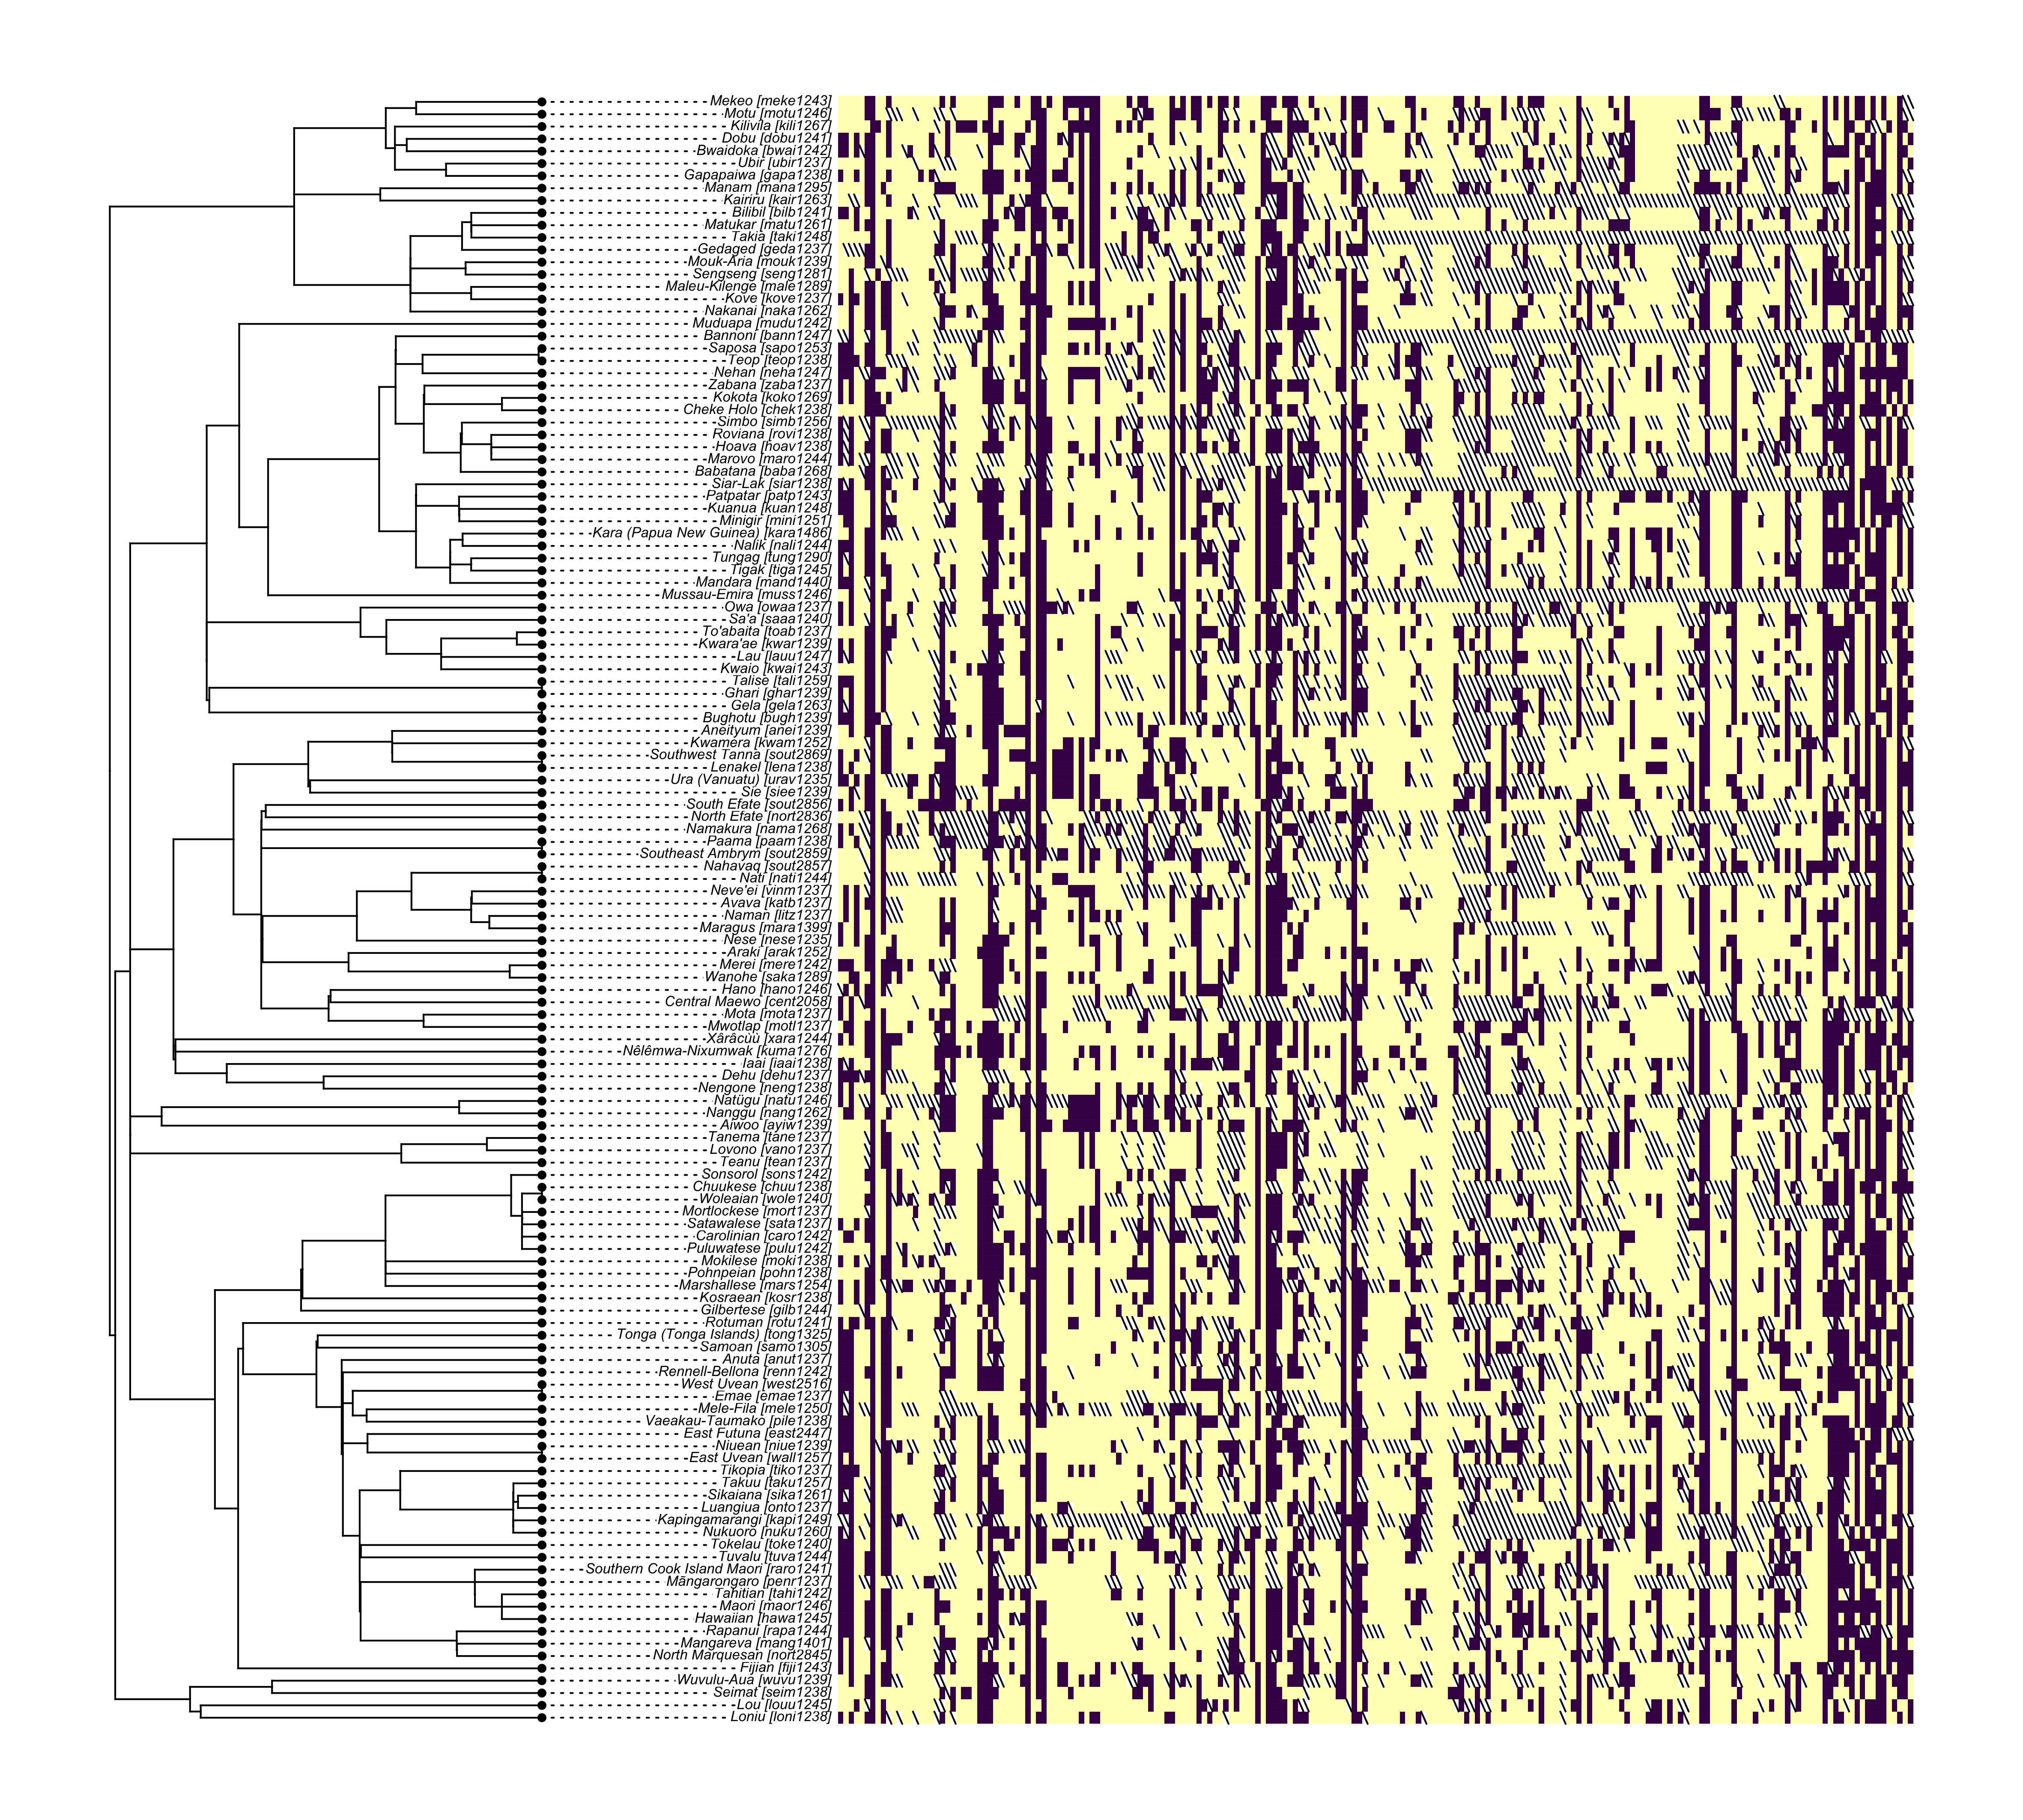
\includegraphics[width=18cm]{illustrations/plots_from_R/coverage_plots/tree_heatmap_gray_mcct.png}
\caption{MCC-tree from \citet{grayetal_2009} with Grambank data matrix. Purple = present, yellow = absent and striped = missing.}
\label{fig:tree_heatmap}
\end{figure}


\FloatBarrier
\newpage
\subsection{Technical details on D-estimation}
\label{supp:d_estimate}
D-estimates are a tool for measuring phylogenetic signal in a set of binary data. Phylogenetic signal can be broadly described as the degree to which the data is generated by a given tree, or whether it was generated by some other process such as randomness. This particular method was proposed by \cite{fritz2010selectivity} and is implemented in the R-package caper by Fritz and Orome \citep{orme2013caper}. 

The method outputs three primary values per dataset and tree: i) a D-estimate, ii) a p-value that represents how similar the data is to 0 (Brownian motion) and iii) the same kind of p-value, but instead in regard to how similar the data is to a D-estimate of 1 (randomness). If the 0-p-value is large (i.e. p>0.05) that means that the D-estimate of the data is \emph{not dissimilar} from 0, in other worse it is \emph{similar}. If we want to find sets of data that are similar to 0, we should look for large 0-p-values (not dissimilar = similar). The same goes for the p-values relating to 1. There can be D-estimates that are similar to both 0 \emph{and} 1 --- or neither.

The method relies on generating two kinds of simulated data: a Brownian threshold process and randomness. It then measures how similar your empirical data is to the Brownian simulation in comparison to how similar the Brownian simulation is to the random simulations. A D-estimate value of 0 represents identity to the Brownian process, 1 to the random process. D-estimates can also be smaller than 0 and larger than 1, and certainly any values in between. 

The results are sensitive to how many random permutations it runs for the second set of simulated data. \cite{fritz2010selectivity} recommends 1,000 permutations, which is also what the default value is set to for the function phylo.d in the R-package caper. However, during the work for this paper we have found further considerations that should be taken into account when working with this method --- specifically in regard to the number of random permutations and skewed distributions.

\subsubsection{D-estimate: Sensitivity to skewed distributions}
\label{sec:SM_phylo_d_sensitive}
While it is true that D-estimates can be smaller than 0 and larger than 1, in my experience values lower than -7 (very strong signal) and larger than 7 (very over-dispersed) are rare in empirical data. Furthermore, we would expect that if we re-run the algorithm a second time using the same data, same tree and same settings we get a similar result to the first time. This is generally true, except in certain specific situations. When the data is such that only one data point has a diverging value from the rest --- for example in a set of 155 tips only one of them has the value 1 for the binary trait and all others 0 --- then the algorithm struggles and produces very different results on each run, and very extreme values such as -10 on one run and 10 on another. This is problematic, and was probably not discovered by \cite{fritz2010selectivity} and \cite{orme2013caper} because their empirical data rarely exhibited this kind of distribution (1 - 154). However, for some of the linguistic features of this study this can indeed happen. 

Having identified the problem, we can also offer two solutions: a) increasing the number of random permutations and/or b) disregard data of this kind. Many thanks to \citep{orme2013caper} for the package documentation of caper and the paper by \cite{fritz2010selectivity} for providing enough methodological detail for this to be diagnosed. Stephen Mann was also invaluable to helping diagnose and address this issue mathematically.

To illustrate the problem I generated a tree with 155 tips with different distributions of binary values. The list below describes the different feature value distributions (with short names used in the plot in parenthesis) and Fig \ref{fig:phylo_d_heatmap} shows the tree and feature value distributions

\begin{itemize}
    \item only one tip of state 1, all other 154 tips 0 (singleton)
        \begin{itemize}
            \item daughter with few splits from the roots (outlier)
            \item in a more nested position (middle)
            \item at a random position (random)
        \end{itemize}
    \item three features with each a pair of direct sister tips of state 1, all other 153 tips 0 (sisters\_a, sisters\_b and sisters\_c)
    \item two random tips with the state 1, all other 0 (two\_random)
    \item three features with each a set of three closely related languages with the state 1, all other 152 tips 0 (triplets\_a, triplets\_b and triplets\_c)
    \item three random tips with the state 1, all other 0 (three\_random)
   \item three features with each a set of four closely related languages with the state 1, all other 151 tips 0 (quadruplets\_a, quadruplets\_b and quadruplets\_c
    \item four random tips with the state 1, all other 0 (four\_random)
    \item a cluster of 31 tips which form a clade all with 1 for the feature, all others 0 (cluster)
    \item 31 random tips with the same state, all others other (cluster\_random)
\end{itemize}

\begin{figure}[!ht]
\centering
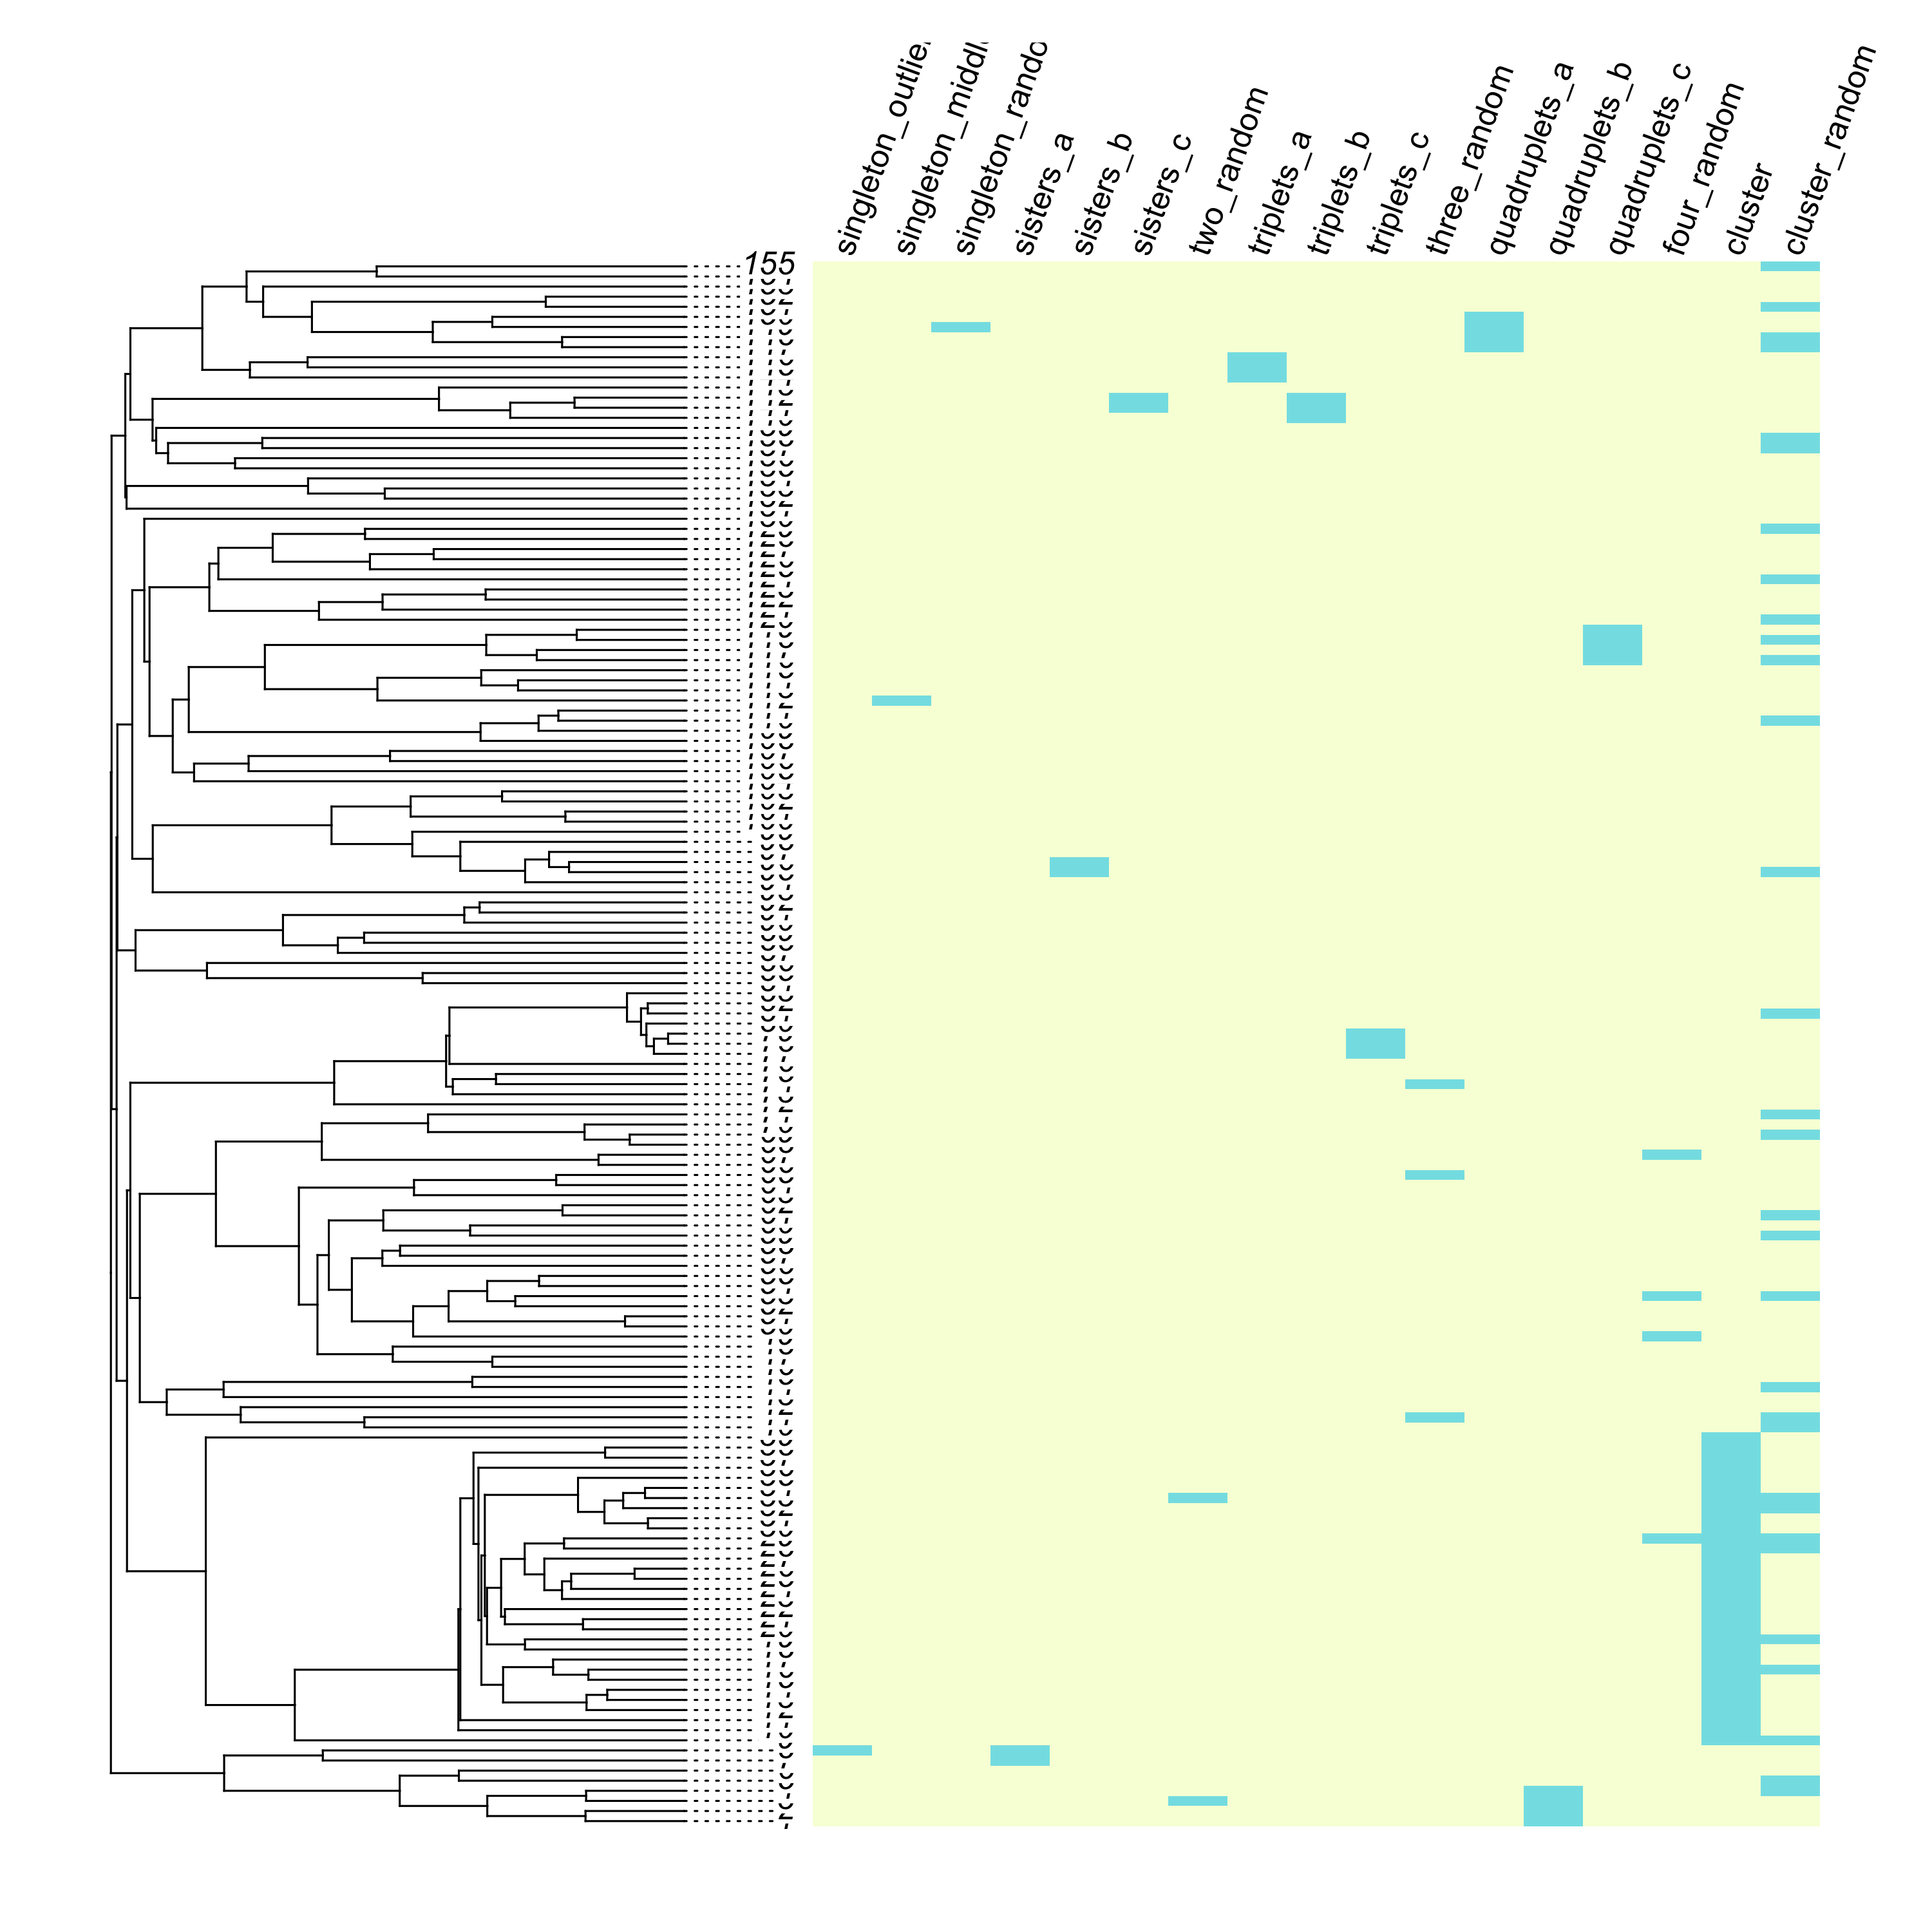
\includegraphics[width=14cm]{illustrations/plots_from_R/phylo_d_heatmap_tree.png}
\caption{Tree and values heatmap for D-estimation investigation.}
\label{fig:phylo_d_heatmap}
\end{figure}

I then proceeded to estimate the D-value for each of these 17 features, varying the number of permutations (1,000, 20,000 and 30,000). I repeated this 8 times, i.e. generating 17 * 3 * 8 D-estimates. For the entire investigation, see the script 11\_phylo\_d\_investigation.R in the accompanying material.

The D-estimates for the singleton-features varied the most, with one iteration of the singleton outlier feature reaching a D-estimate value of 1,520 (sic). This value occurred when the number of permutations was set to 1,000. In another iteration over the same feature and the same number of iterations, the D-estimate came out as -21. While it is potentially plausible to get very small or very large values, we would expect to get \emph{similar} values with each iteration given the same data and settings. The difference between a positive value of 1,520 and a negative of -21 is surely \emph{unreasonably} large. When the number of permutations was increased beyond 1,000, the variance of the output with each iteration was reduced (see Fig \ref{fig:phylo_d_plot_sd}), but it was still noticeably larger in cases where the distribution was heavily skewed.

\begin{figure}[!ht]
\centering
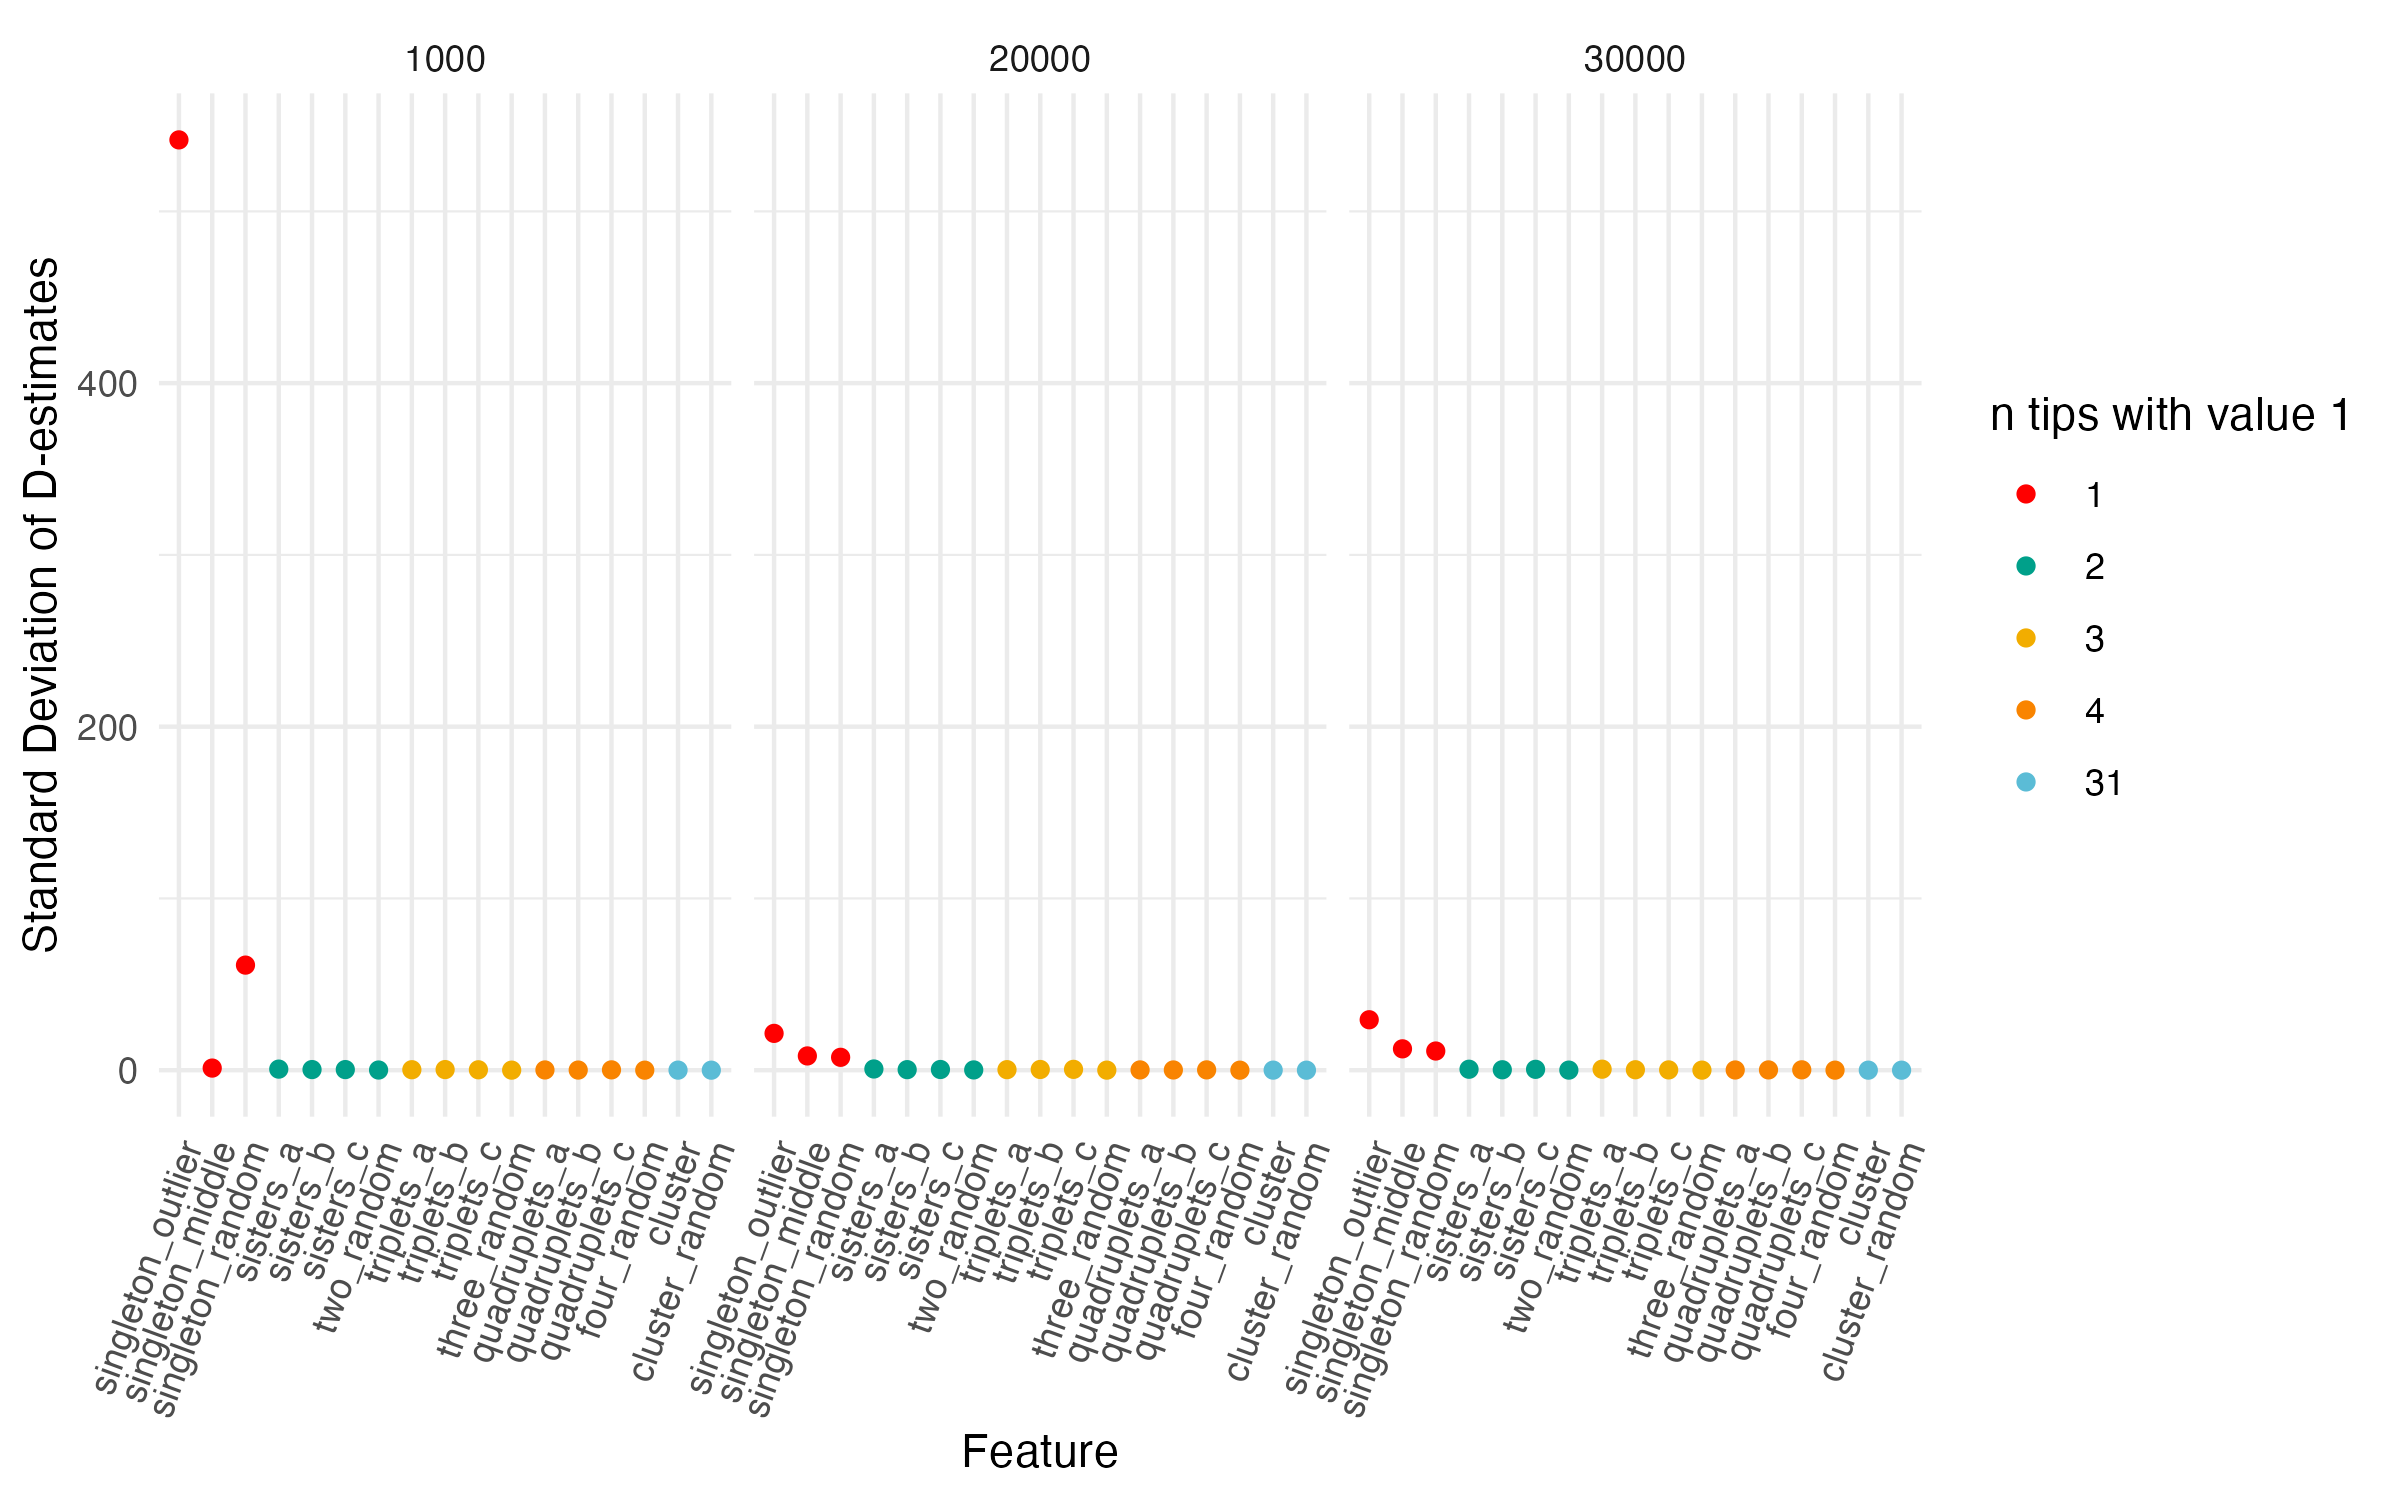
\includegraphics[width=14cm]{illustrations/plots_from_R/phylo_d_sd_permut.png}
\caption{Scatterplot of the standard deviation of D-estimate values per feature per value of random permutations}
\label{fig:phylo_d_plot_sd}
\end{figure}

The cause of this issue with wildly varying D-estimates each run, especially when the feature value distribution is very skewed, has to do with the chance of generating a particular pattern of 1/154 \emph{precisely} versus 4/151. Each time the D-estimate process is applied, a set of random and Brownian simulations are generated (the number is set by the permutations value). If the data is of the kind where 1 tip differs from all the other 154 tips (as for a few of the features in the toy example above), there is a chance that that particular position of that one value occurs in at least one of the random cases. If it does happen to occur, we would get a D-estimate that signals randomness --- and conversely if it happens to be similar to the Brownian evolutionary model. If the random and Brownian simulations end up being similar the denominator (see Eq. \ref{eq_d_estimate}) in the formula becomes very small, which can lead to very large absolute values for the D-estimate (such as the 1,520 we saw earlier). In Eq. \ref{eq_d_estimate}) \citep{fritz2010selectivity} r = random, b = brownian and obs = observed data.

\begin{align}
\label{eq_d_estimate}
    \text{D} 
         &=  \frac{\sum\emph{d}_{obs} - mean(\sum\emph{d}_{b})} {mean(\sum\emph{d}_{r}) - mean(\sum\emph{d}_{b})}
\end{align}

There is less of a chance of this happening if we have more tips in each state, because those are more complicated patterns that are less likely to occur exactly in the simulated processes. Because of the possibility of this irrelevant similarity, it is necessary to increase the number of simulated permutations so that we have a larger pool of things to compare our data to. This is why the D-estimate standard deviation stabilise more in cases with skewed feature distributions if the number of permutations is increased (see Fig \ref{fig:phylo_d_plot_sd}).

%The Brownian, observed and random distributions of values are more likely to happen to be similar the more skewed the feature value distribution is, as was said earlier it is easier to happen to have 1 value out of 155 in the same positions in a tree than, for example, 54 values. There are more unique configurations of a 54 - 101 value distribution over the tips than 1 - 154.

Even when the number of permutations is increased to 30,000, the instances where there is a feature distribution of 1 - 154 (singeltons) are more volatile than the rest. When using this technique, it may be necessary to set aside such cases and evaluate them separately from the rest. We may want to ask ourselves: what does it mean for something that does not even form a pair to have or not have a phylogenetic signal?

If we look at the non-singleton features (the pairs, triplets, quadruplets and larger group) in the simulation example explored here in Fig. \ref{fig:phylo_d_plot_non_singles} we see that they behave more similarly with each iteration. Even an increase from 1 to 2 tips of the same state improves the performance of this method in terms of producing a similar value each iteration.

\begin{figure}[ht]
\centering
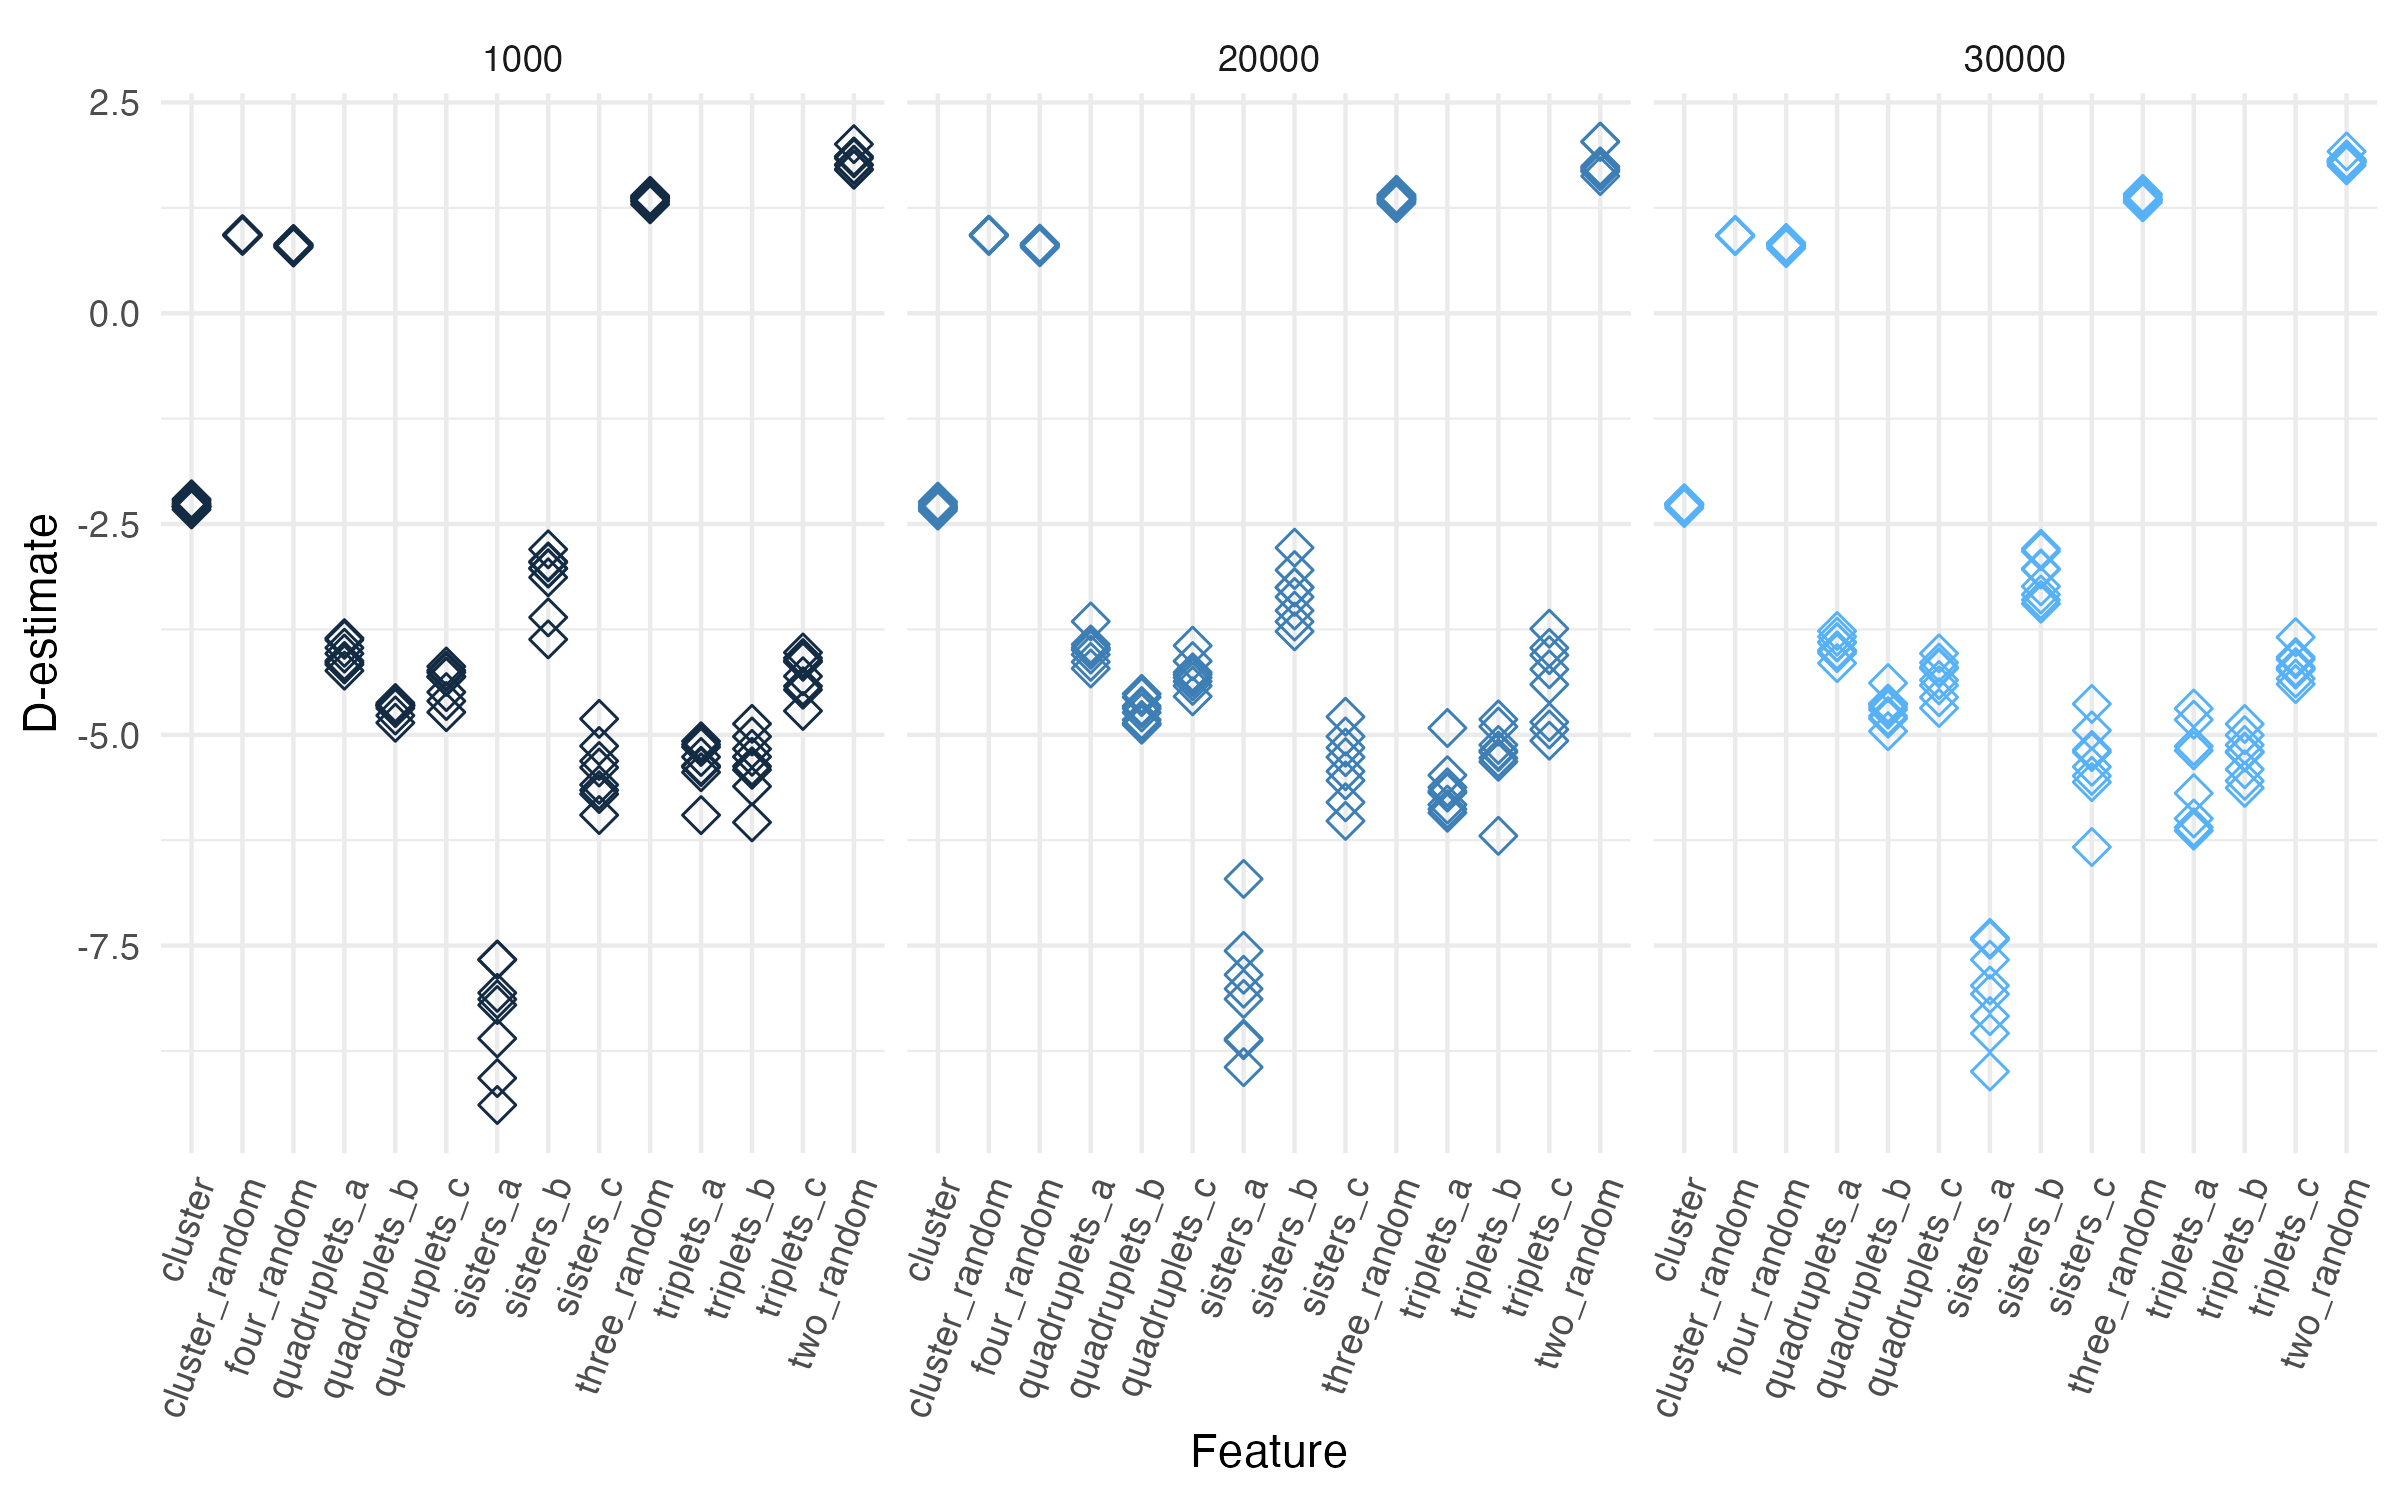
\includegraphics[width=14cm]{illustrations/plots_from_R/phylo_d_permut_plot.png}
\caption{Scatterplot of the D-estimate values per feature per value of random permutations, for all non-singleton features. Each point represents a D-estimate value per feature, per number of permutations and per iteration.}
\label{fig:phylo_d_plot_non_singles}
\end{figure}

In the data in this study there were cases of inappropriate D-estimates, which were possible to diagnose both by the extremity of the D-estimates, but also by examining the p-values (dissimilarity to 0 / 1). We grouped the output into 2 groups, with 4 sub-groups each. The output in the second group is not possible to include in the analysis because the conditions do not meet the model requirements, it is either impossible to conduct the analysis (all tips one state), would generate seriously unreliable results (singleton states) or shows evidence of Brownian and random being similar which also throw suspicion on the outcome. In all four cases of the kinds of data that is not possible to include the distribution of tips over the two states is heavily skewed. For future work, it would be desirable if the function also output a p-value which represents the dissimilarity between the random and Brownian simulations and generated a warning when the distributions are heavily skewed (for example, only 5\% tips in one state). 


\begin{itemize}
    \item \colorbox{spec_color_lightgreen!50}{possible to include in analysis}
    \begin{enumerate}[label=(\roman*)]
     \item p-values indicate similarity to Brownian only
      \item p-values indicate similarity to random only
      \item p-values indicate similarity to both random and Brownian, D-estimate is between 0 and 1
      \item p-values indicate \emph{dis}similarity to both random and Brownian, D-estimate is between 0 and 1
    \end{enumerate}
    \item \colorbox{spec_color_orange!50}{\emph{not} possible to include in analysis}
    \begin{enumerate}[label=(\roman*)]
        \item all tips same state (phylo.d does not even run)
        \item singleton
        \item p-values indicate similarity to both Brownian and random, D-estimate is above 1
        \item p-values indicate similarity to both Brownian and random, D-estimate is below 0
    \end{enumerate}
    
\end{itemize}

Tables \ref{phylo_d_summarise_col_green} and \ref{phylo_d_summarise_col_orange} shows the number of instances of each of these categories over the trees. There are fewer instances in the problematic categories and they have been excluded from further analysis with D-estimates directly. Because they represent cases with skewed distributions, it is possible to interpret them as representing very rare phenomena and one interpretation of that could be a strong phylogenetic signal --- but the D-estimate test is not suitable.

% latex table generated in R 4.2.2 by xtable 1.8-4 package
% Wed Mar 15 22:58:17 2023
\begin{table}[ht]
\centering
\begin{tabular}{p{3cm}p{3cm}p{3cm}p{3cm}p{3cm}}
  \toprule
tree & $\textbf{\cellcolor{spec_color_lightgreen!50}{\parbox{2.7cm}{\raggedright similar to 0}}}$ & $\textbf{\cellcolor{spec_color_lightgreen!50}{\parbox{2.7cm}{\raggedright similar to both, between 0 \& 1}}}$ & $\textbf{\cellcolor{spec_color_lightgreen!50}{\parbox{2.7cm}{\raggedright similar to 1}}}$ & $\textbf{\cellcolor{spec_color_lightgreen!50}{\parbox{2.7cm}{\raggedright dissimilar to both, between 0 \& 1}}}$ \\ 
  \midrule
glottolog & 59 & 9 & 28 & 75 \\ 
  Gray (2009) - mcct & 76 & 23 & 44 & 20 \\ 
  Gray (2009) - posteriors & 89 & 37 & 24 & 2 \\ 
   \bottomrule
\end{tabular}
\caption{Table of types of D-estimates per tree, data-points included.} 
\label{phylo_d_summarise_col_green}
\end{table}


% latex table generated in R 4.2.2 by xtable 1.8-4 package
% Thu Jan 26 14:56:37 2023
\begin{table}[h]
\centering
\begin{tabular}{p{3cm}p{3cm}p{3cm}p{3cm} p{3cm}}
  \toprule
tree & $\textbf{\cellcolor{spec_color_orange!50}{\parbox{2.7cm}{\raggedright all same}}}$ & $\textbf{\cellcolor{spec_color_orange!50}{\parbox{2.7cm}{\raggedright one off}}}$ & $\textbf{\cellcolor{spec_color_orange!50}{\parbox{2.7cm}{\raggedright similar to both, above 1}}}$ & $\textbf{\cellcolor{spec_color_orange!50}{\parbox{2.7cm}{\raggedright similar to both, below 0}}}$ \\ 
  \midrule
glottolog & 0 & 2 & 2 & 1 \\ 
  Gray (2009) - mcct & 1 & 3 & 2 & 4 \\ 
  Gray (2009) - posterior & 1 & 3 & 2 & 7 \\ 
   \bottomrule
\end{tabular}
\caption{Table of types of D-estimates per tree, data-points not included.} 
\label{phylo_d_summarise_col, orange}
\end{table}



%#todo
\FloatBarrier


\subsubsection{Correlation D-estimate and HL-concurrence}
\label{supp:cor_d_HL}
Phylogenetic signal could be an indication that it is easier to reconstruct a prior state. One may for example consider that it ought to be more difficult to reconstruct a state reliably if the pattern is a random phylogenetic signal (D-estimate similar to 1), and conversely that a strong signal may make it easier to reconstruct consistently, and therefore that the agreement between conventional historical linguistics findings and the computational methods applied in this paper would be higher if the phylogenetic signal is strong (=similar to 0, Brownian). This is however not the case in this study.

Fig. \ref{fig:phylo_d_plot_vs_concurrence} shows the D-estimate on the x-axis (low = strong signal, high = random) and agreement with conventional historical linguistics on the y-axis. The agreement with HL is the precise value that the method predicted for the state that HL suggests. If HL suggests that the state is present at a particular node, and the computational suggests that presence has a likelihood of 0.435, the agreement value is 0.435. This is a continuous scale, but for the parsimony results it is often 0, 0.5 or 1 because of the prevalence of binary splits in the tree and the way the method works.

The results have been grouped by method and tree. In no case, save one, does the correlation reach the conventional threshold for statistical significance for the Pearson correlation (p > 0.05). The exception is Parsimony - Glottolog tree, and even there the correlation is weak (0.23). Furthermore, the correlation is positive which is the opposite of what we would expect. If strong phylogenetic signal (low D-estimate) predicts high agreement, then the correlation would be negative. 

\begin{figure}[ht]
\centering
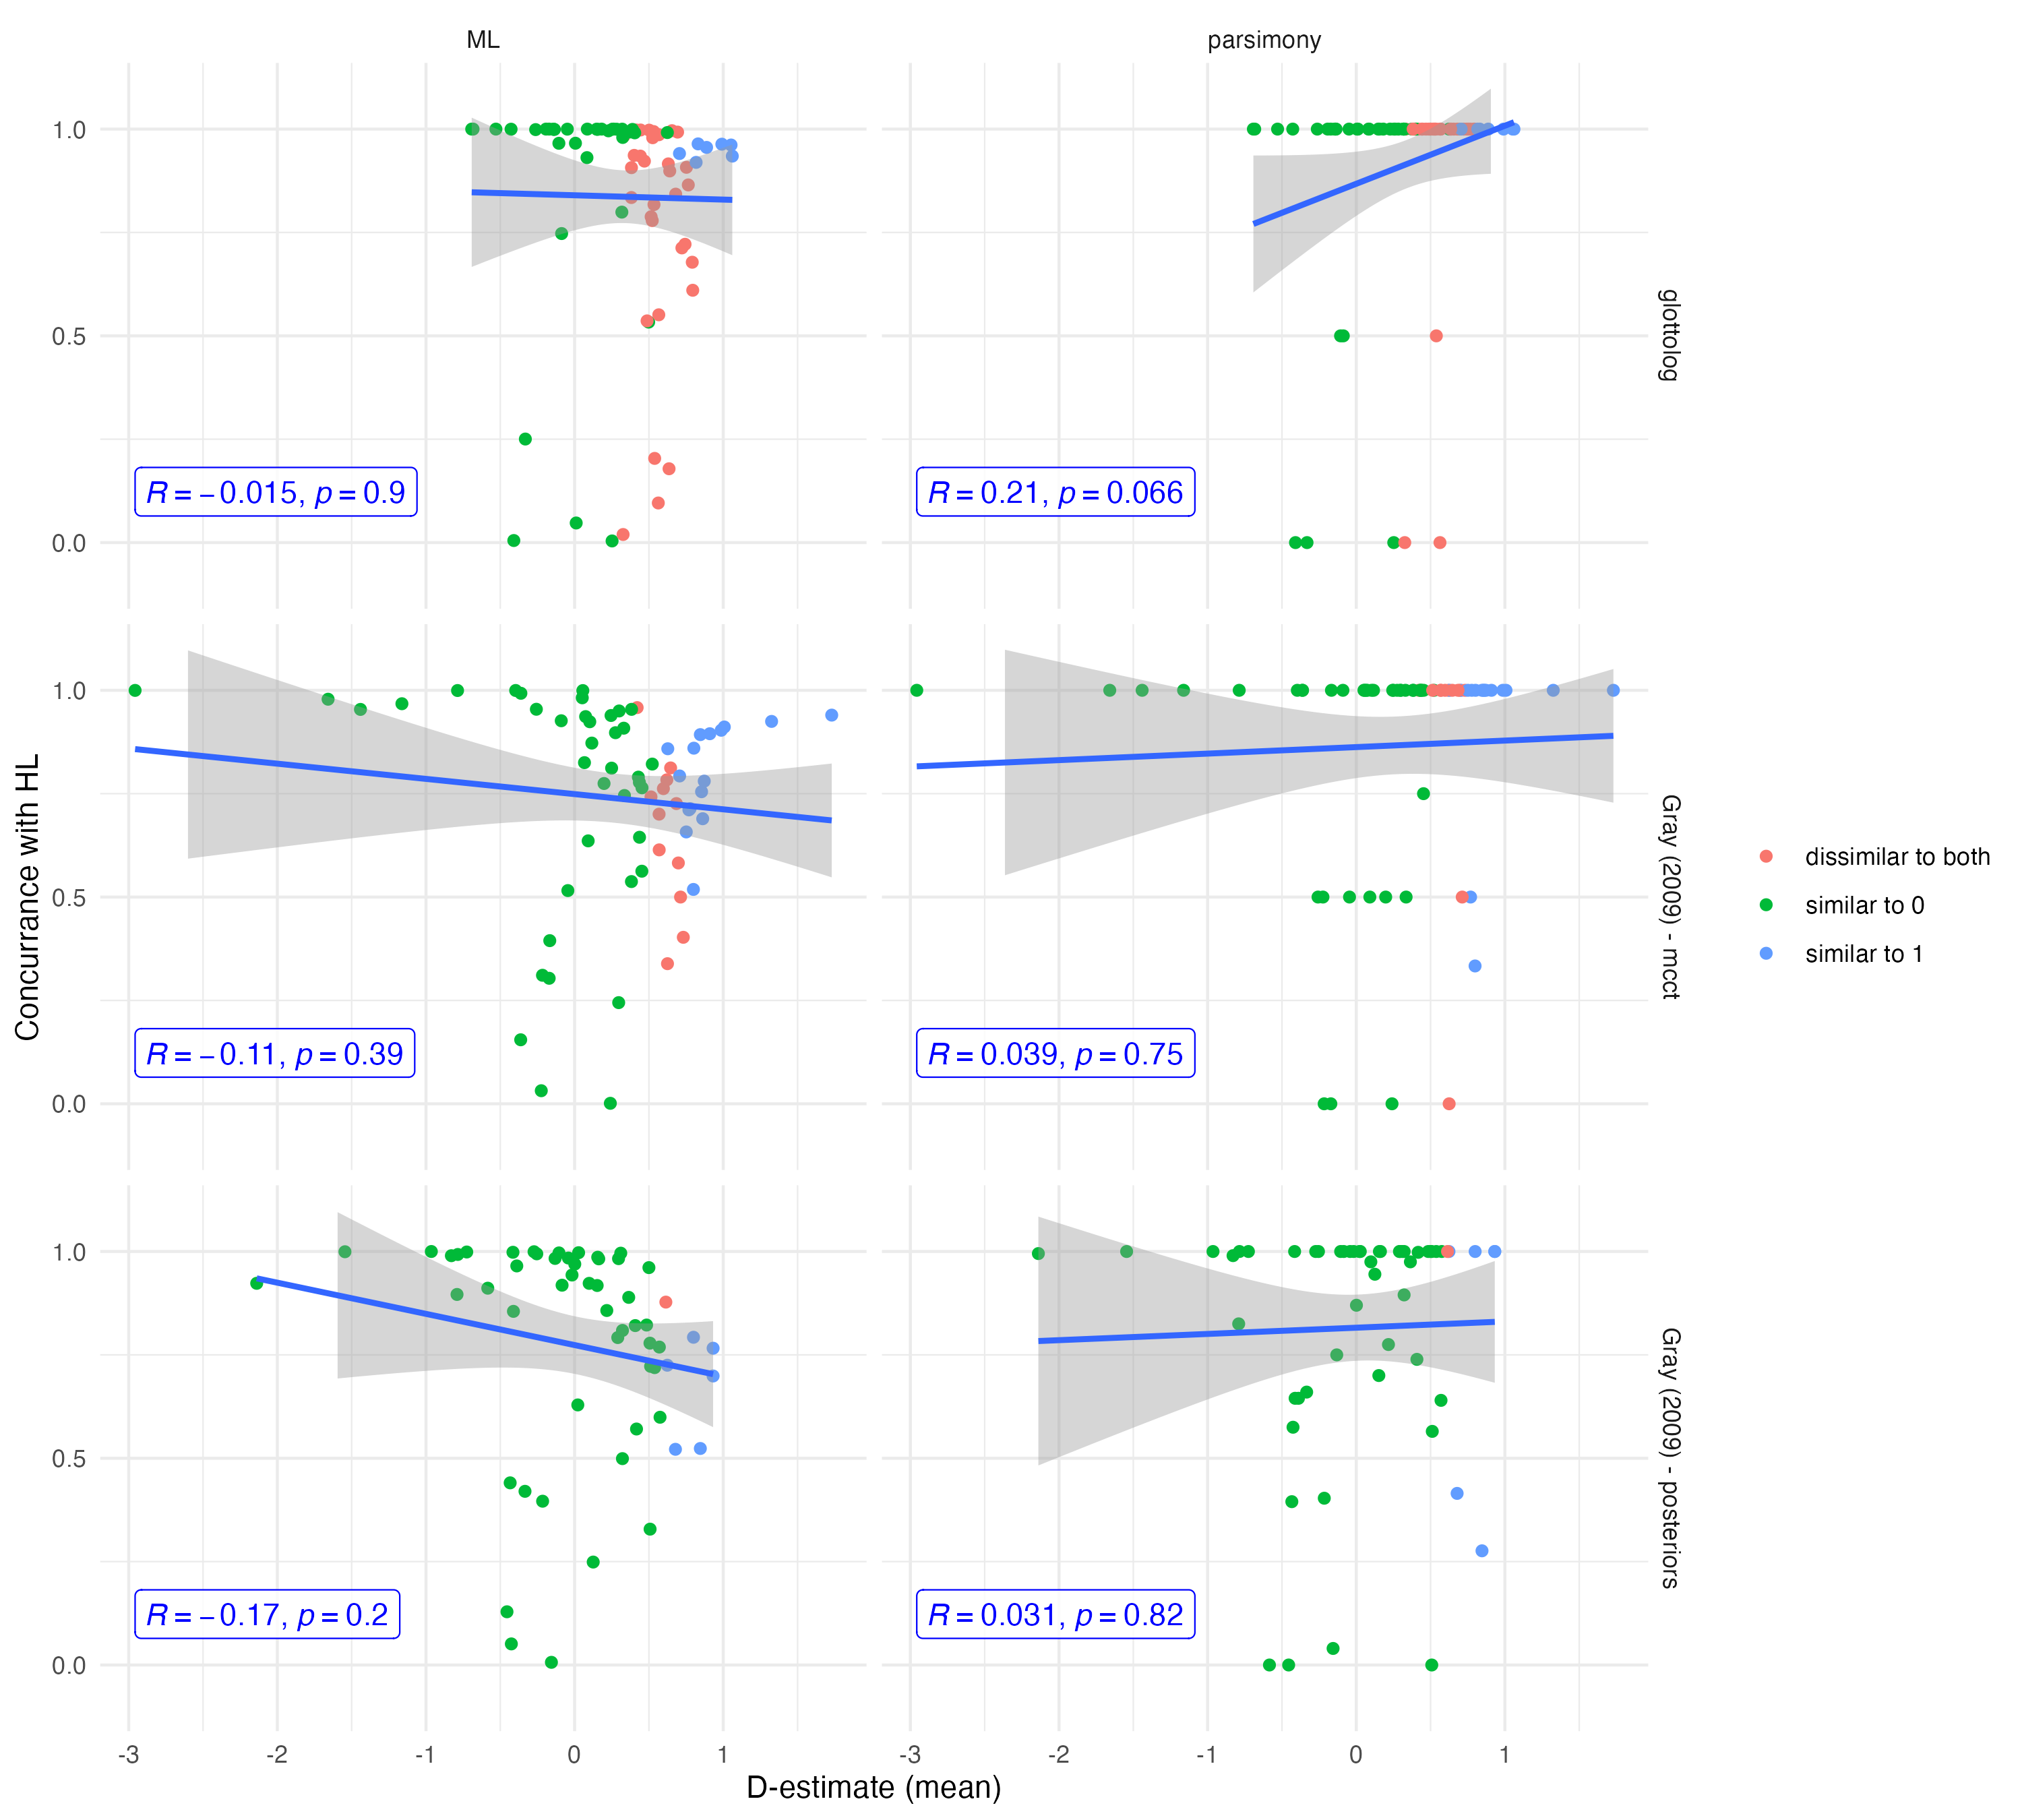
\includegraphics[width=18cm]{illustrations/plots_from_R/phylo_d_vs_HL_concurrance.png}
\caption{Scatter-plots of D-estimates (x-axis) and concurrence with conventional historical linguistics (y-axis). The points are colored based on meeting statistical thresholds of significance for being similar to 0 (Brownian) or 1 (random). The correlation statistic in blue represents a Pearson-test.}
\label{fig:phylo_d_plot_vs_concurrence}
\end{figure}

Each point is mapped onto one prediction of one feature and one proto-language (Proto-Oceanic, Proto-Central Pacific, Proto-Polynesian or Proto-Eastern Polynesian), but the D-estimate is only taken for the entire Oceanic tree, not for each sub-clade. The predictions for "most common" were excluded, since there is not a tree \emph{per se} which the D-estimate can take as input to measure the phylogenetic signal. In addition, we also excluded data-points that were ill-fitting for other reasons as discussed in the previous section.

\FloatBarrier

\subsection{Correlation value distributions and HL-concurrence}
\label{supp:cor_min_p_HL}
We can consider a much simpler approach to understanding what predicts agreement between the computational methods and historical linguists --- the number of tips in each state, then we see some stronger patterns. The idea is that if very few tips are in one state and all others in the other, there is little variation that can drive disagreements between the different reconstructions. If on the other hand, the states are distributed 50\%/50\% then it is reasonable to assume there is a greater chance for disagreement. In fig  \ref{fig:min_p_vs_concurrence}, the x-axis is the percentage of tips in the minority state --- 0\% indicates that all tips are of the same state (be that presence or absence) and 50\% that half of the tips are in one state, half in another. 30\% indicates that the state with the fewest tips had 30\% of the tips. The y-axis represents concurrence with traditional historical linguistics. Each point is one structural feature in one of the four proto-languages.

\begin{figure}[ht]
\centering
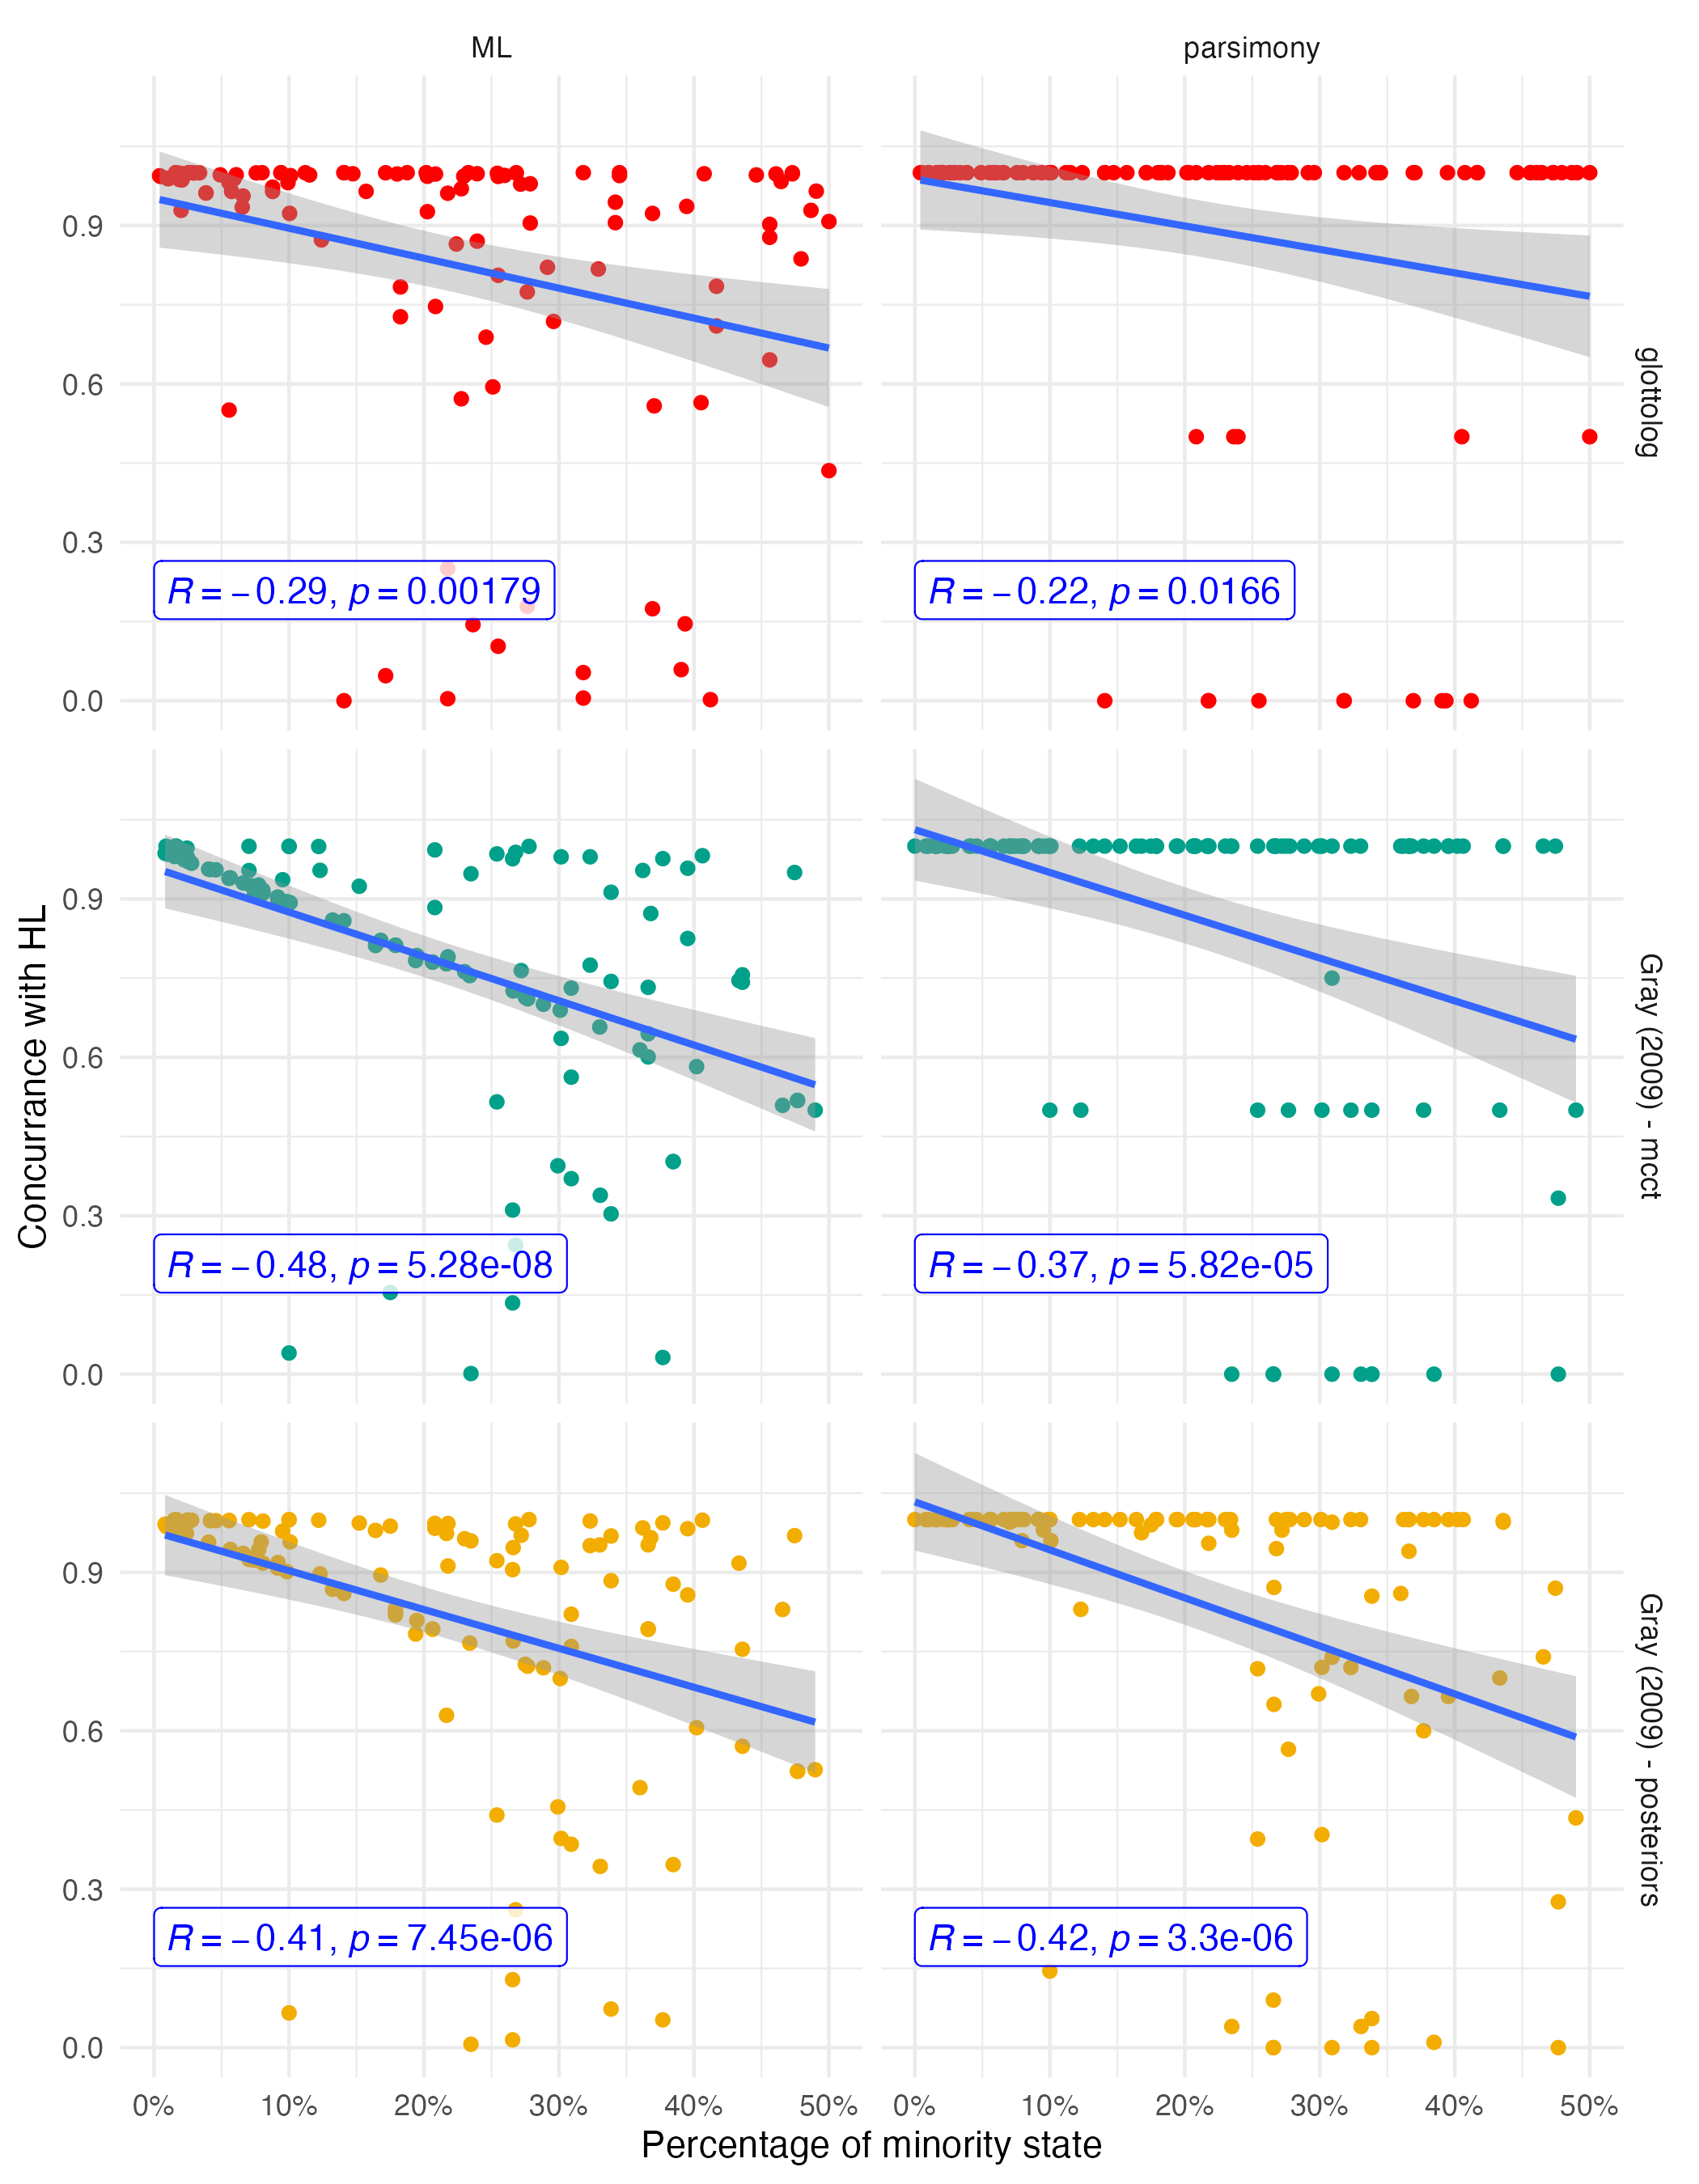
\includegraphics[width=12cm]{illustrations/plots_from_R/min_p_vs_HL_concurrance.png}
\caption{Scatter-plots of precentage of tips in minority state (x-axis) and concurrence with conventional historical linguistics (y-axis). The correlation statistic in blue represents a Pearson-test.}
\label{fig:min_p_vs_concurrence}
\end{figure}

All of the comparisons between HL-concurrence and the percentage of tips in minority state have a p-value lower than 0.05, which is a commonly used cut-off for significance. All correlations are negative, which is to be expected. This indicates that when tips are more evenly distributed between the two states (closer to 50\% on the x-axis), there is more disagreement between each of the methods and traditional HL. Most correlations are weak (between 0.2 and 0.39), and a few are of moderate strength (between 0.40 - 0.59). There are some outliers in the lower left quadrant of the plot, these represent cases where most tips are in one state and yet there is a disagreement. One of them is discussed in greater detail in the following section.

\FloatBarrier

\subsection{Disagreement between methods detail: present, 50\%/50\% versus absent}
\label{supp:GB133_detail}
One example of disagreement between conventional HL, Maximum Parsimony and Maximum Likelihood is GB133 `Is a pragmatically unmarked constituent order verb-final for transitive clauses?` for Proto-Oceanic. This feature has a very low concurrence with HL for the ML method (0.04) and \citep{grayetal_2009}) MCC-tree, despite the tip state distribution being 10\%/90\% which we saw in the previous section usually predicts high agreement.

Let us first consider the historical linguistics literature and the feature at hand. The coding of Proto-Oceanic as present for this feature according to conventional historical linguistics is based on the following passage from \citet{pawley1973some}:

\begin{quotation}
\noindent\emph{
Capell's suggestion that the SOV order found in many New Guinea Oceanic languages is the result of influence by Papuan (non-Austronesian) languages, almost all of which show SOV order, seems reasonable. }[..]\emph{
Still, the fact that the better-known SVO languages also tolerate certain other orders (for non- pronominal constituents) suggests that some variation occurred in POC} [Proto-Oceanic]\emph{. In particular, occurrences of OSV and VOS order are widely distributed enough to indicate that both were possible in POC.}\footnote{Pawley does note that the ``basic'' word order in Proto-Oceanic is likely to be SVO (Subject-Verb-Object).}
\end{quotation} \begin{flushright}\citet[118]{pawley1973some}\end{flushright}

Unlike the chapter in the World Atlas of Language Structures on order in the transitive clause \citep{wals-81}, the Grambank feature questionnaire does not ask about the ``dominant''-type, but has 3 different binary questions about the ``pragmatically unmarked'' order. 

{\small
\begin{itemize}
    \item GB131 Is a pragmatically unmarked constituent order verb-initial for transitive clauses?
    \item GB132 Is a pragmatically unmarked constituent order verb-medial for transitive clauses?
    \item GB133 Is a pragmatically unmarked constituent order verb-final for transitive clauses?
\end{itemize}

 }
 
It is possible for a language to be answered ``yes'' for more than one question if multiple orders occur (without changing the pragmatics). However, most Oceanic languages were still coded as absent for GB133. The Maximum Parsimony and Maximum Likelihood all disagree with conventional HL regarding GB133 for Proto-Oceanic - but in different ways.

Fig \ref{fig:parsimony_gray_mcct} shows the Ancestral Nodes of GB133 on the Gray et al (2009)-MCCT with the parsimony method, and Fig \ref{fig:ML_gray_mcct} the same tree but with the Maximum Likelihood method. These two tree figures have the same exact topology and tip states, they only vary in the reconstruction of internal nodes (proto-languages). In each of the figures, there is a set of languages at the bottom of the tree that are coded as "yes" for  GB133 and these are located on the island of New Guinea or nearby. Their location in the tree is such that they form a clade that is an early offshoot from the root. For the parsimony method, that means that even though most of the tips are of another state, this group carries a lot of weight. The parsimony method suggests that the state of the root, of Proto-Oceanic, is 50\%/50\%. However, the Maximum Likelihood method takes into account branch lengths and the overall tendency in the tree for the trait value "absent" to be stable (because it estimates rates, unlike MP which assumes symmetric rates). This results in a ML-estimation of proto-Oceanic as overwhelmingly absent of verb-finality.

\begin{figure}[ht]
\centering
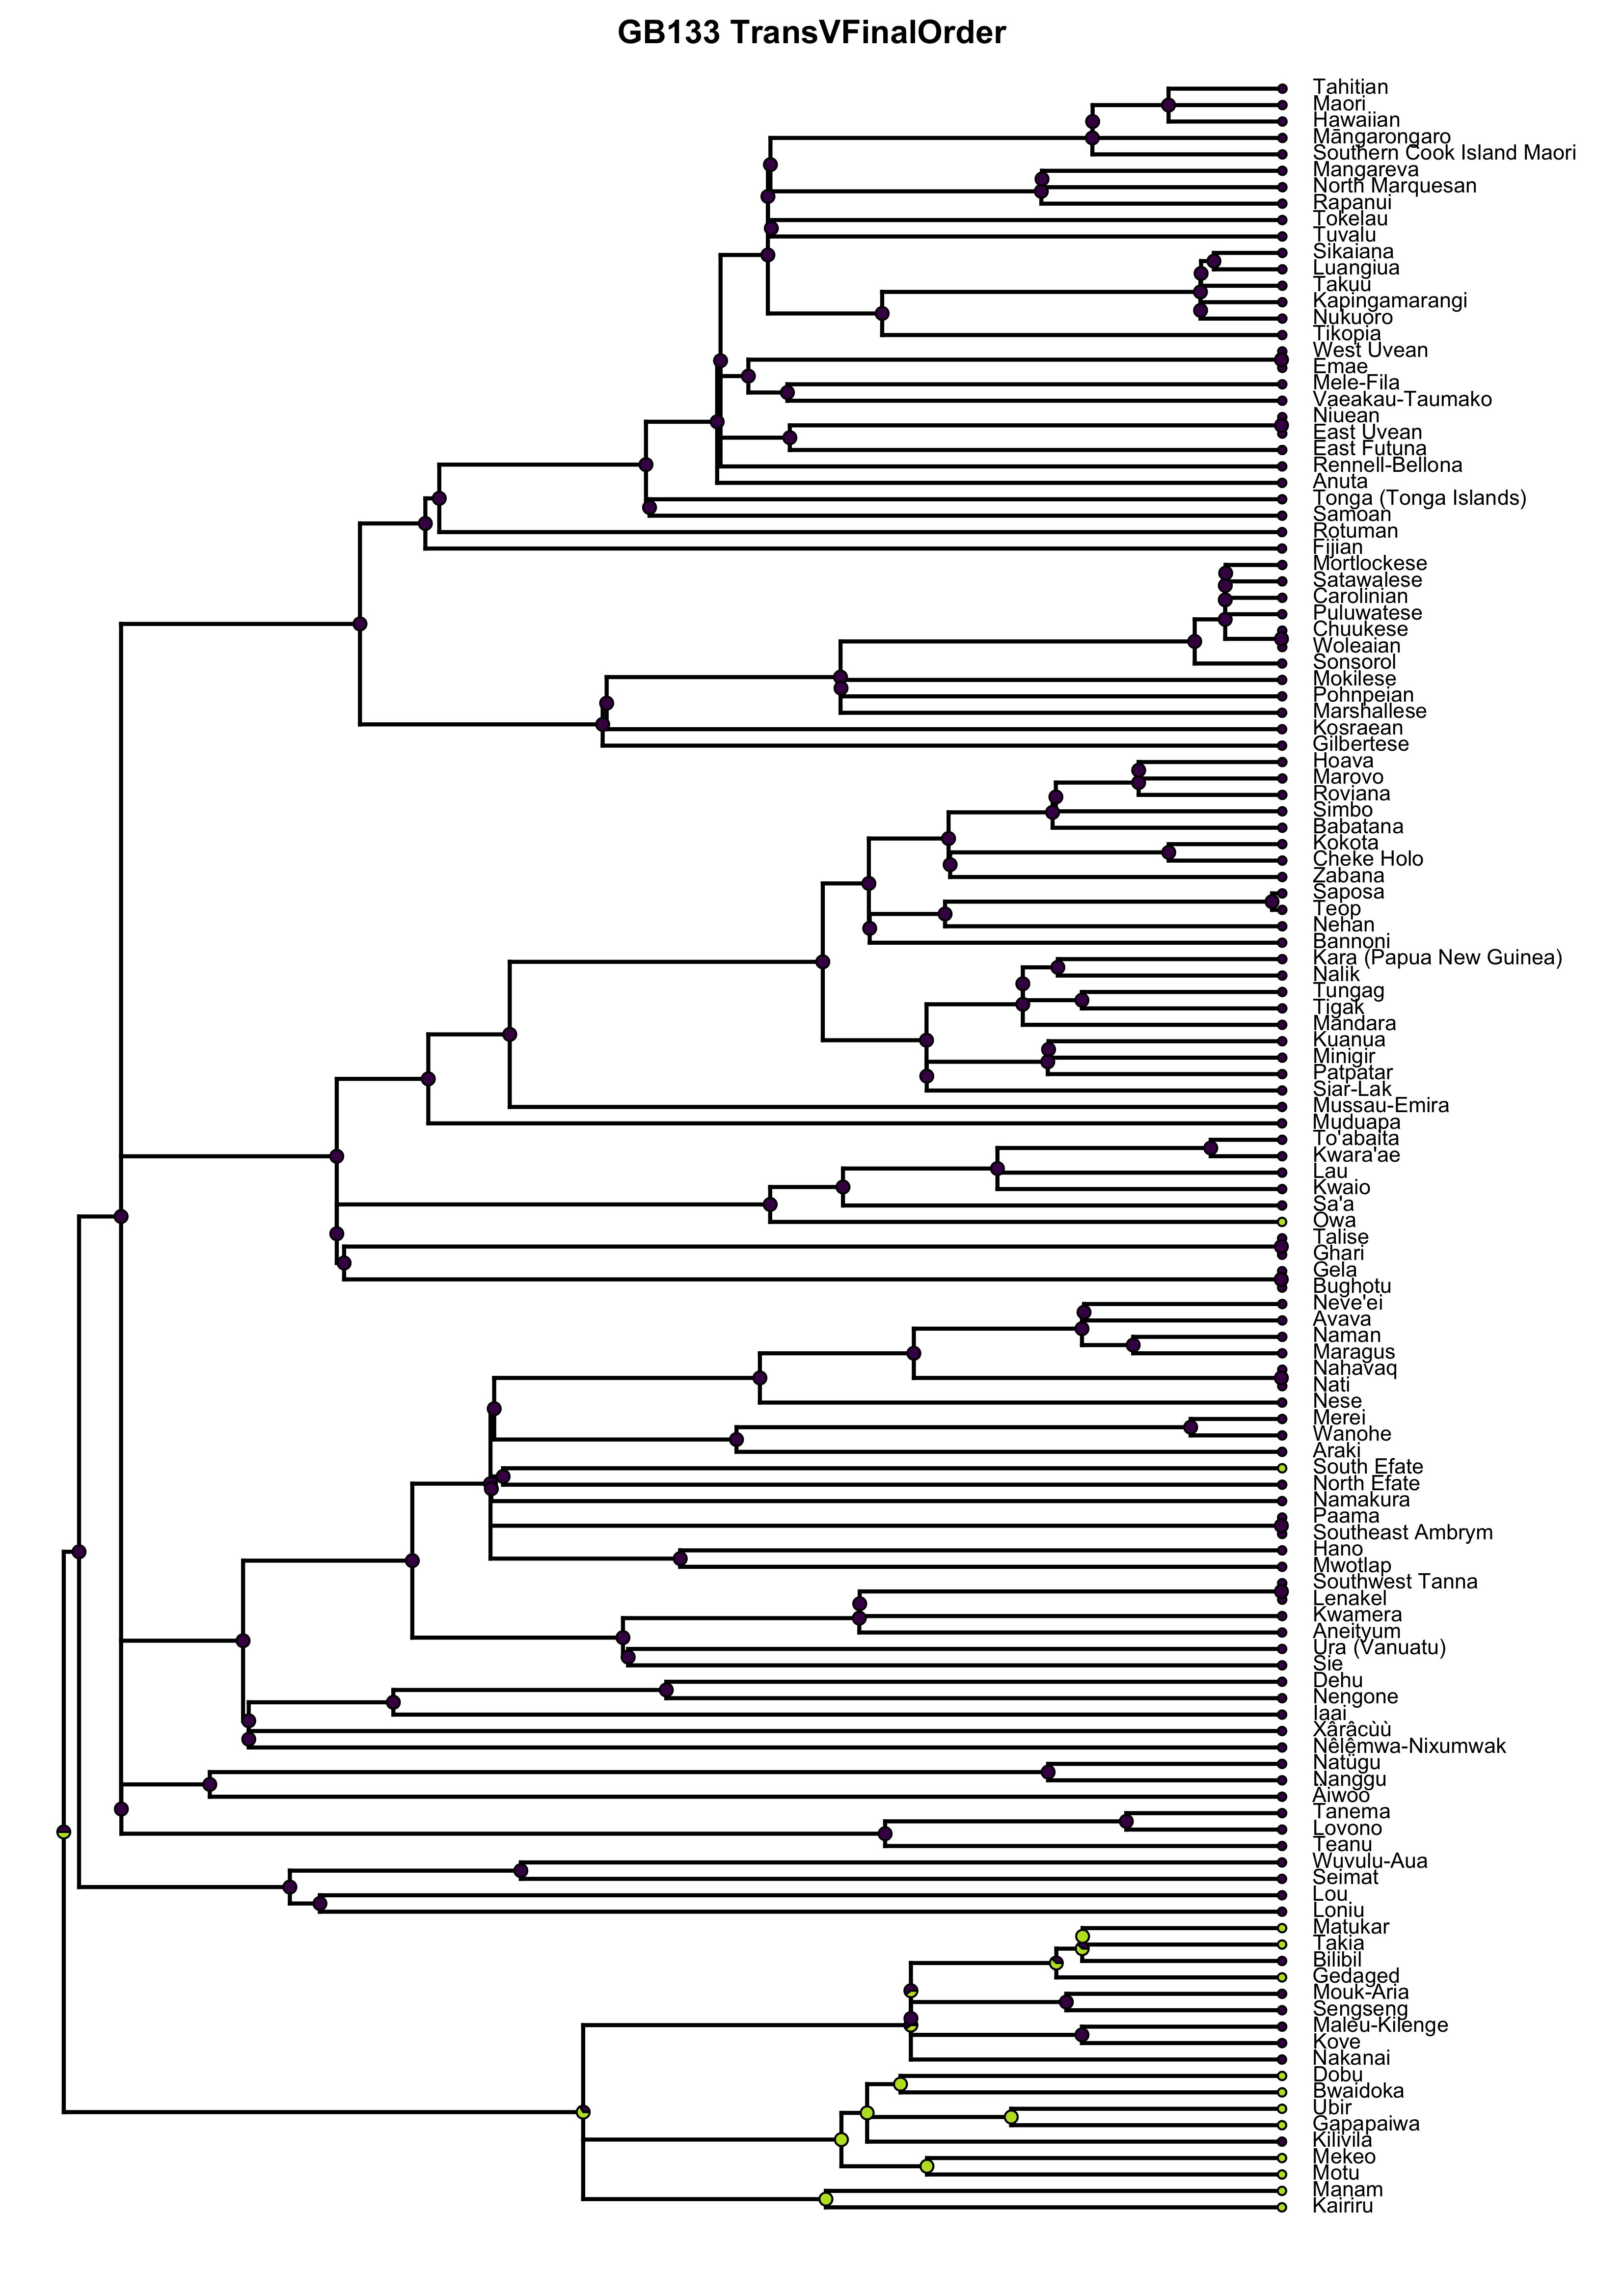
\includegraphics[width=14cm]{illustrations/plots_from_R/tree_plots/gray_et_al_2009/parsimony/parsimony_gray_tree_mcct_GB133.png}
\caption{Gray et al 2009-tree with Maximum Parsimony method, Proto-Oceanic is reconstructed as half/half present/absent. Green = absent, purple = present. Root edge added in for visualisation purposes only.}
\label{fig:parsimony_gray_mcct}
\end{figure}

\begin{figure}[ht]
\centering
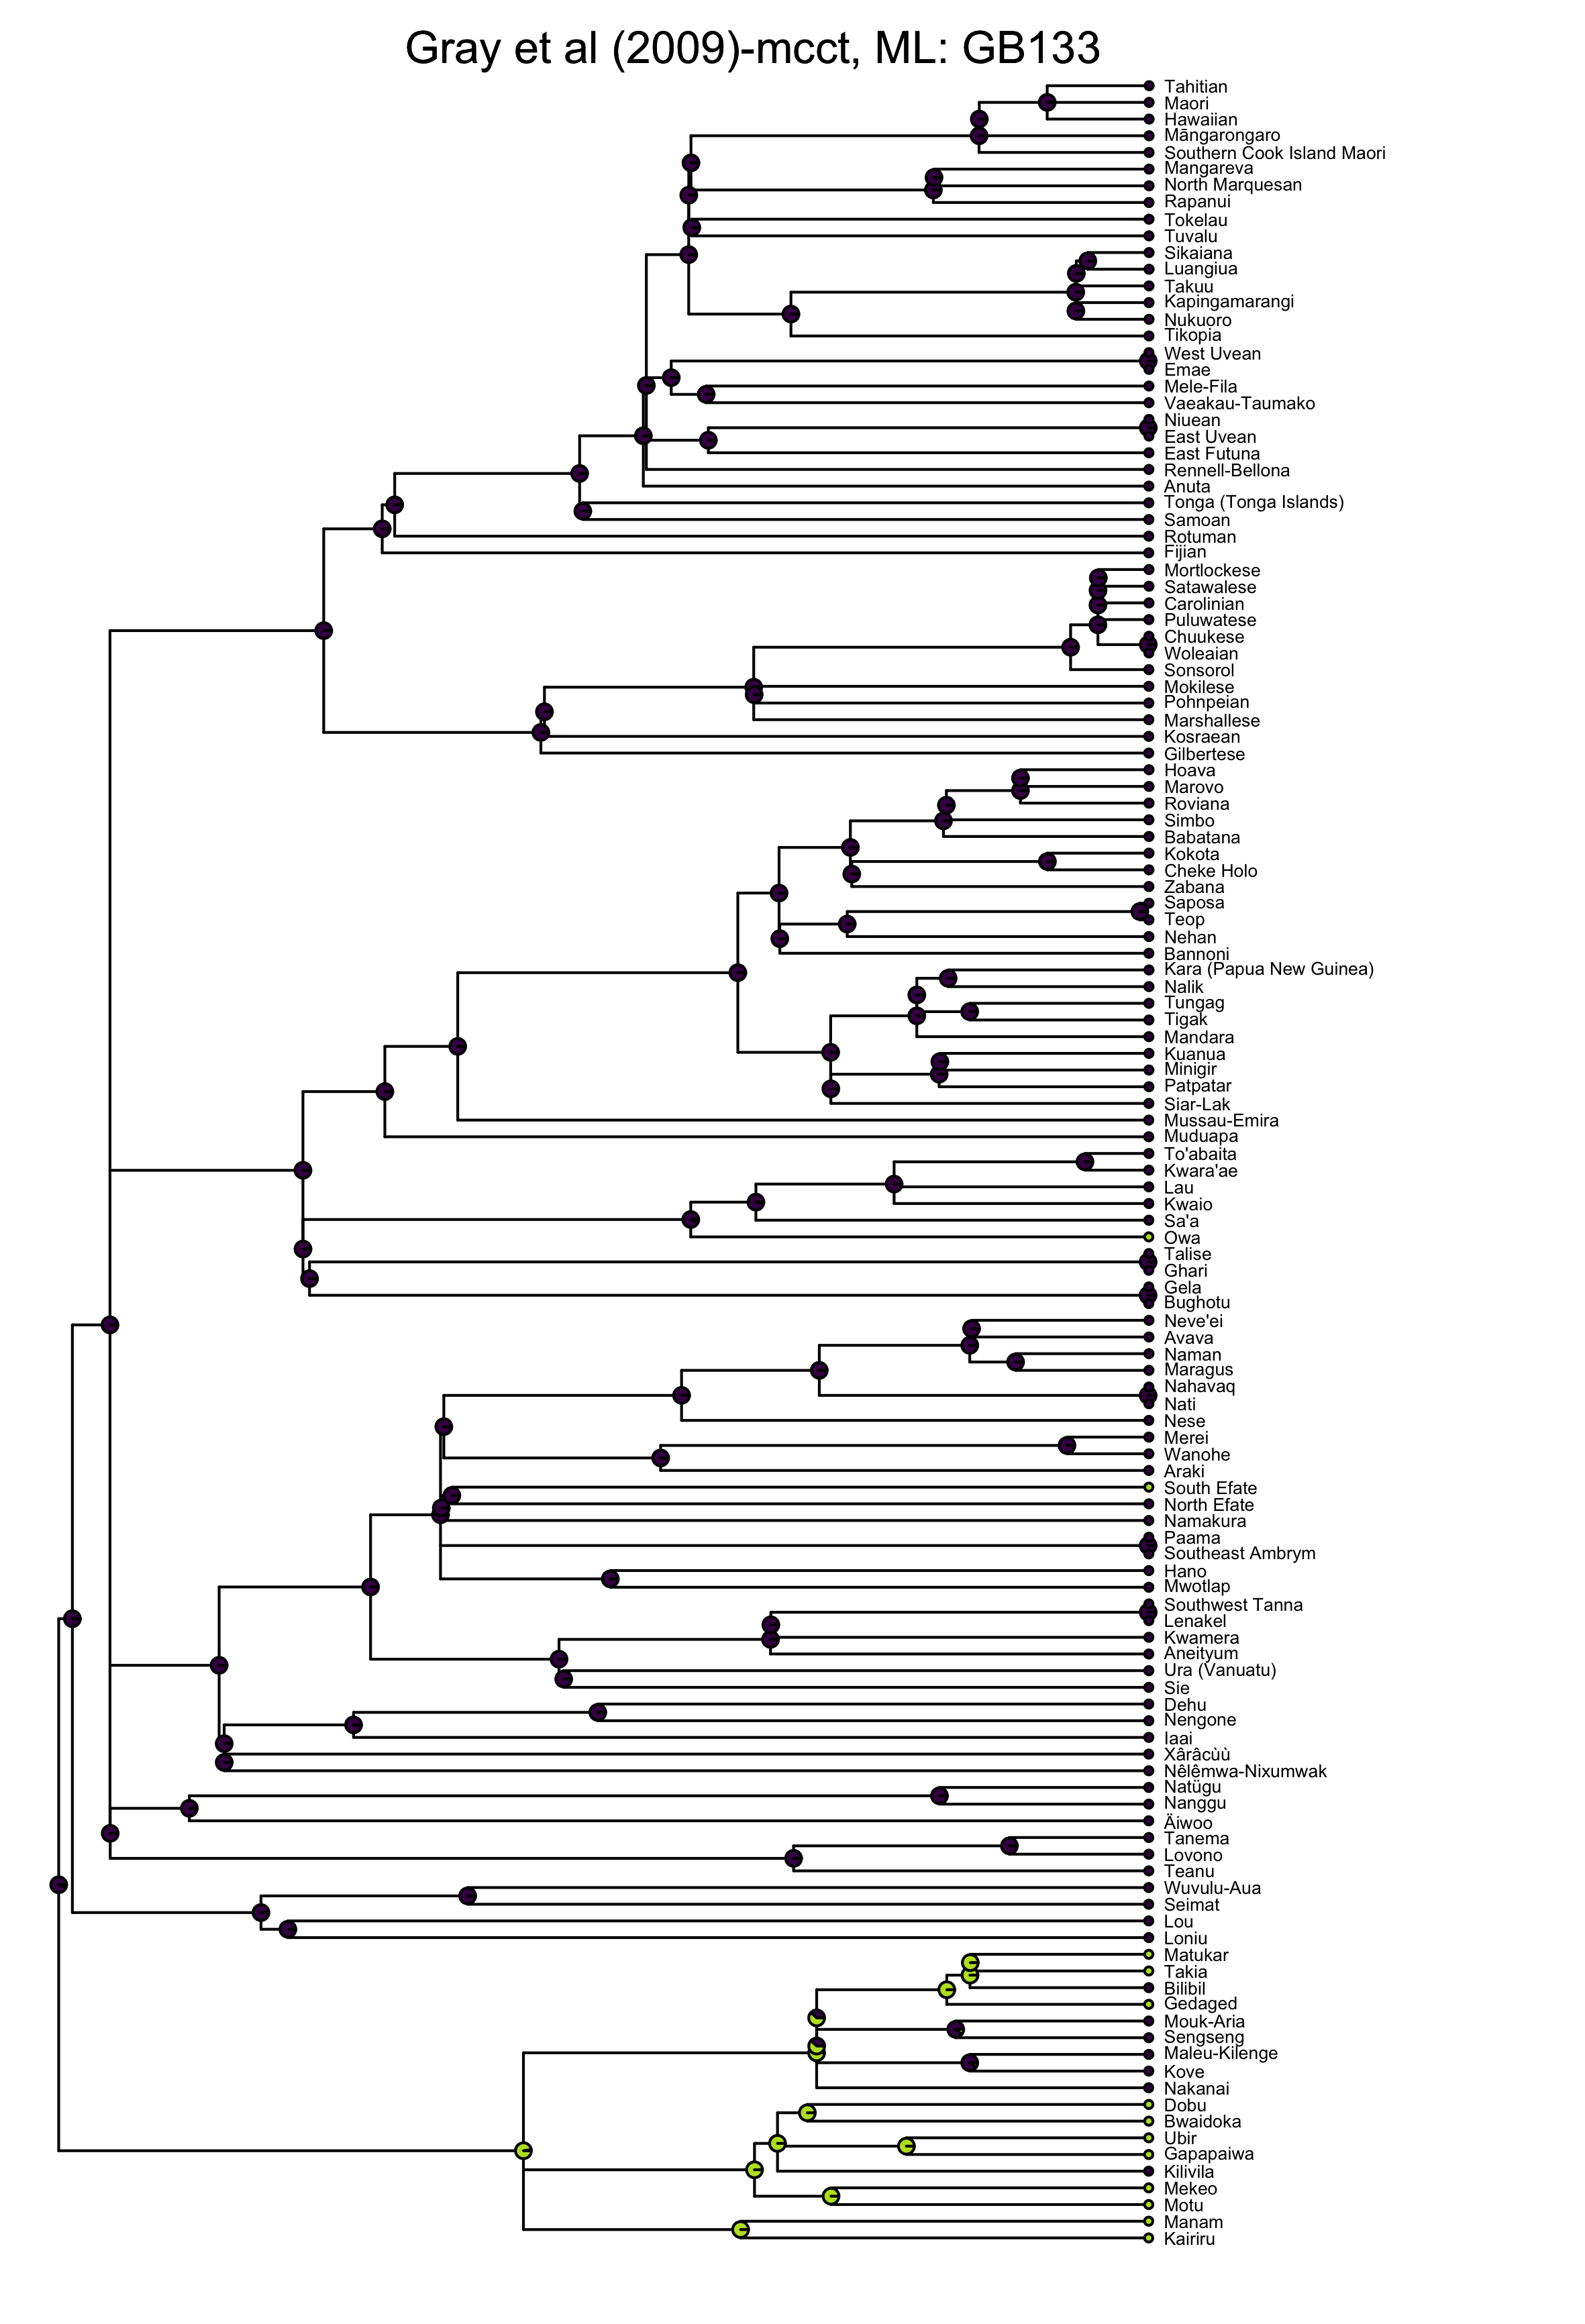
\includegraphics[width=14cm]{illustrations/plots_from_R/tree_plots/gray_et_al_2009/ML/ML_gray_mcct_-GB133.png}
\caption{Gray et al 2009-tree with ML method, Proto-Oceanic is reconstructed as absent.  Green = absent, purple = present. Root edge added in for visualisation purposes only.}
\label{fig:ML_gray_mcct}
\end{figure}

%
%



%Even when you set the number of permutations to 3000, the variation for cases where there is only one singleton tip is still pretty high (579 in my example), and the variance is also quite high for the cases of 2 and 4 cases compared to the case where a larger cluster exists.
%
%image
%If you want to dig deeper, there are also systematic differences if the singleton value is in a more or less direct daughter to the root (“outlier” in my code), smack in the middle or at a random position. It has to do with the way it does ancestral state reconstruction, which is through Felsenstein’s contrasting algorithm (sort of like max parsimony but smarter because it cares about branch lengths).
%
%The R-code I’ve uploaded doesn’t require you to download any data or anything, the tree and data are all there directly in the script. It doesn’t take that long time to run, and when it’s done it’ll do a little “pling!”. You can easily try it out and poke around yourself in the resulting data-frame.
%
%Solution
%
%If you are getting D-estimates that are varying wildly, first take a close look at your feature value distributions. Consider increasing the number of permutations to reign it in a bit.
%
%However, there’s something fundamental you need to consider if you’ve got very skewed data: in order for the D-measure to work, it needs groups of tips to latch onto, clumps. One tip is not a group. Two tips is better, but still a bit sus. You may want to disregard the D-estimates in such cases entirely, and separate those instances out in your data and compare and summarised them in a different way. Set them aside in one bucket and present them in some other way, and compare D-estimates of features that are more suited for this kind of analysis. Have a think about it, have a poke around - run the D-estimate many times and have a look at the variance you get.
%
%Good luck!
%
%P.S. Big thanks to my wonderfully smart husband Stephen (left below) for helping me work out the mathematics of all of this. He is a kind and intelligent person.

\FloatBarrier


\subsection{F1-score results}
\label{f1_results}

F1-scores are the harmonic mean of the precision and recall\footnote{Precision is True Positives divided by True Positives + False Positives, recall is True Positives divided by False Negatives + True Positives. F1-score = 2 * ((precision*recall) / (precision + recall)) \citep{van1979information}.} \citep[133]{van1979information}. It is important to note that F1-scores disregard the number of True Negatives entirely, which is relevant in our case since some of the features in proto-languages are predicted to be absent. For both measures, 0 is the worst possible score and 1 the best in terms of similarity to predictions by historical linguists. 

In a similar study of ancestral states of cognate classes, \citet{jager2018using} compared three different methods of ancestral state reconstruction for lexical data (cognate classes): Maximum Parsimony, Maximum Likelihood and Minimal Lateral Networks. They found that reconstructions using Maximum Likelihood performed the most like the predictions by historical linguists. However, \citet{jager2018using} describe the general performance of all the computational reconstruction methods they used as ``poor''. \citet{jager2018using} evaluated the methods using the F1-score. The highest F1-score was 0.79 (Austronesian language sample, Maximum Likelihood), and the worst was 0.44 (Indo-European, Minimal Lateral Networks).

The formula for F1-scores is given in Eq. \ref{eq:F1_score}.

\begin{equation}\label{eq:F1_score}
\frac{\text{True Positive} }
{\text{True Positive} + \frac{1}{2}\times(\text{False Positive} + \text{False Negative})}
%\caption{Formula for F1-score}
\end{equation}

As stated in section \ref{result_calc_section}, the half-results are also interesting, the formula for F1-scores including half-results is given in Eq. \ref{eq:F1_score_incl_half}. For more on the caluclation of the F1-score including half results, see Supplementary Material \ref{math_supp}.

\begin{equation}\label{eq:F1_score_incl_half}
\frac{\text{True Positive} +  \frac{\text{Half}}{2}} 
{\text{True Positive} + \frac{1}{2}\times(\text{False Positive} + \text{False Negative}) + \text{Half}}
%\caption{Formula for F1-score including half-results}
\end{equation}

The results of the F1-scores are shown in Fig \ref{barplot_facet_results_incl_f1}, alongside the concordance scores. The result for the plain F1-score differs from the other three, this is precisely because it ignores True Negatives. While True Negatives are not included \emph{per se} in the calculation of F1 including half-results score, the inclusion of the half-similarity still has an impact as it makes all the methods more similar.

\begin{figure}[p]
\centering
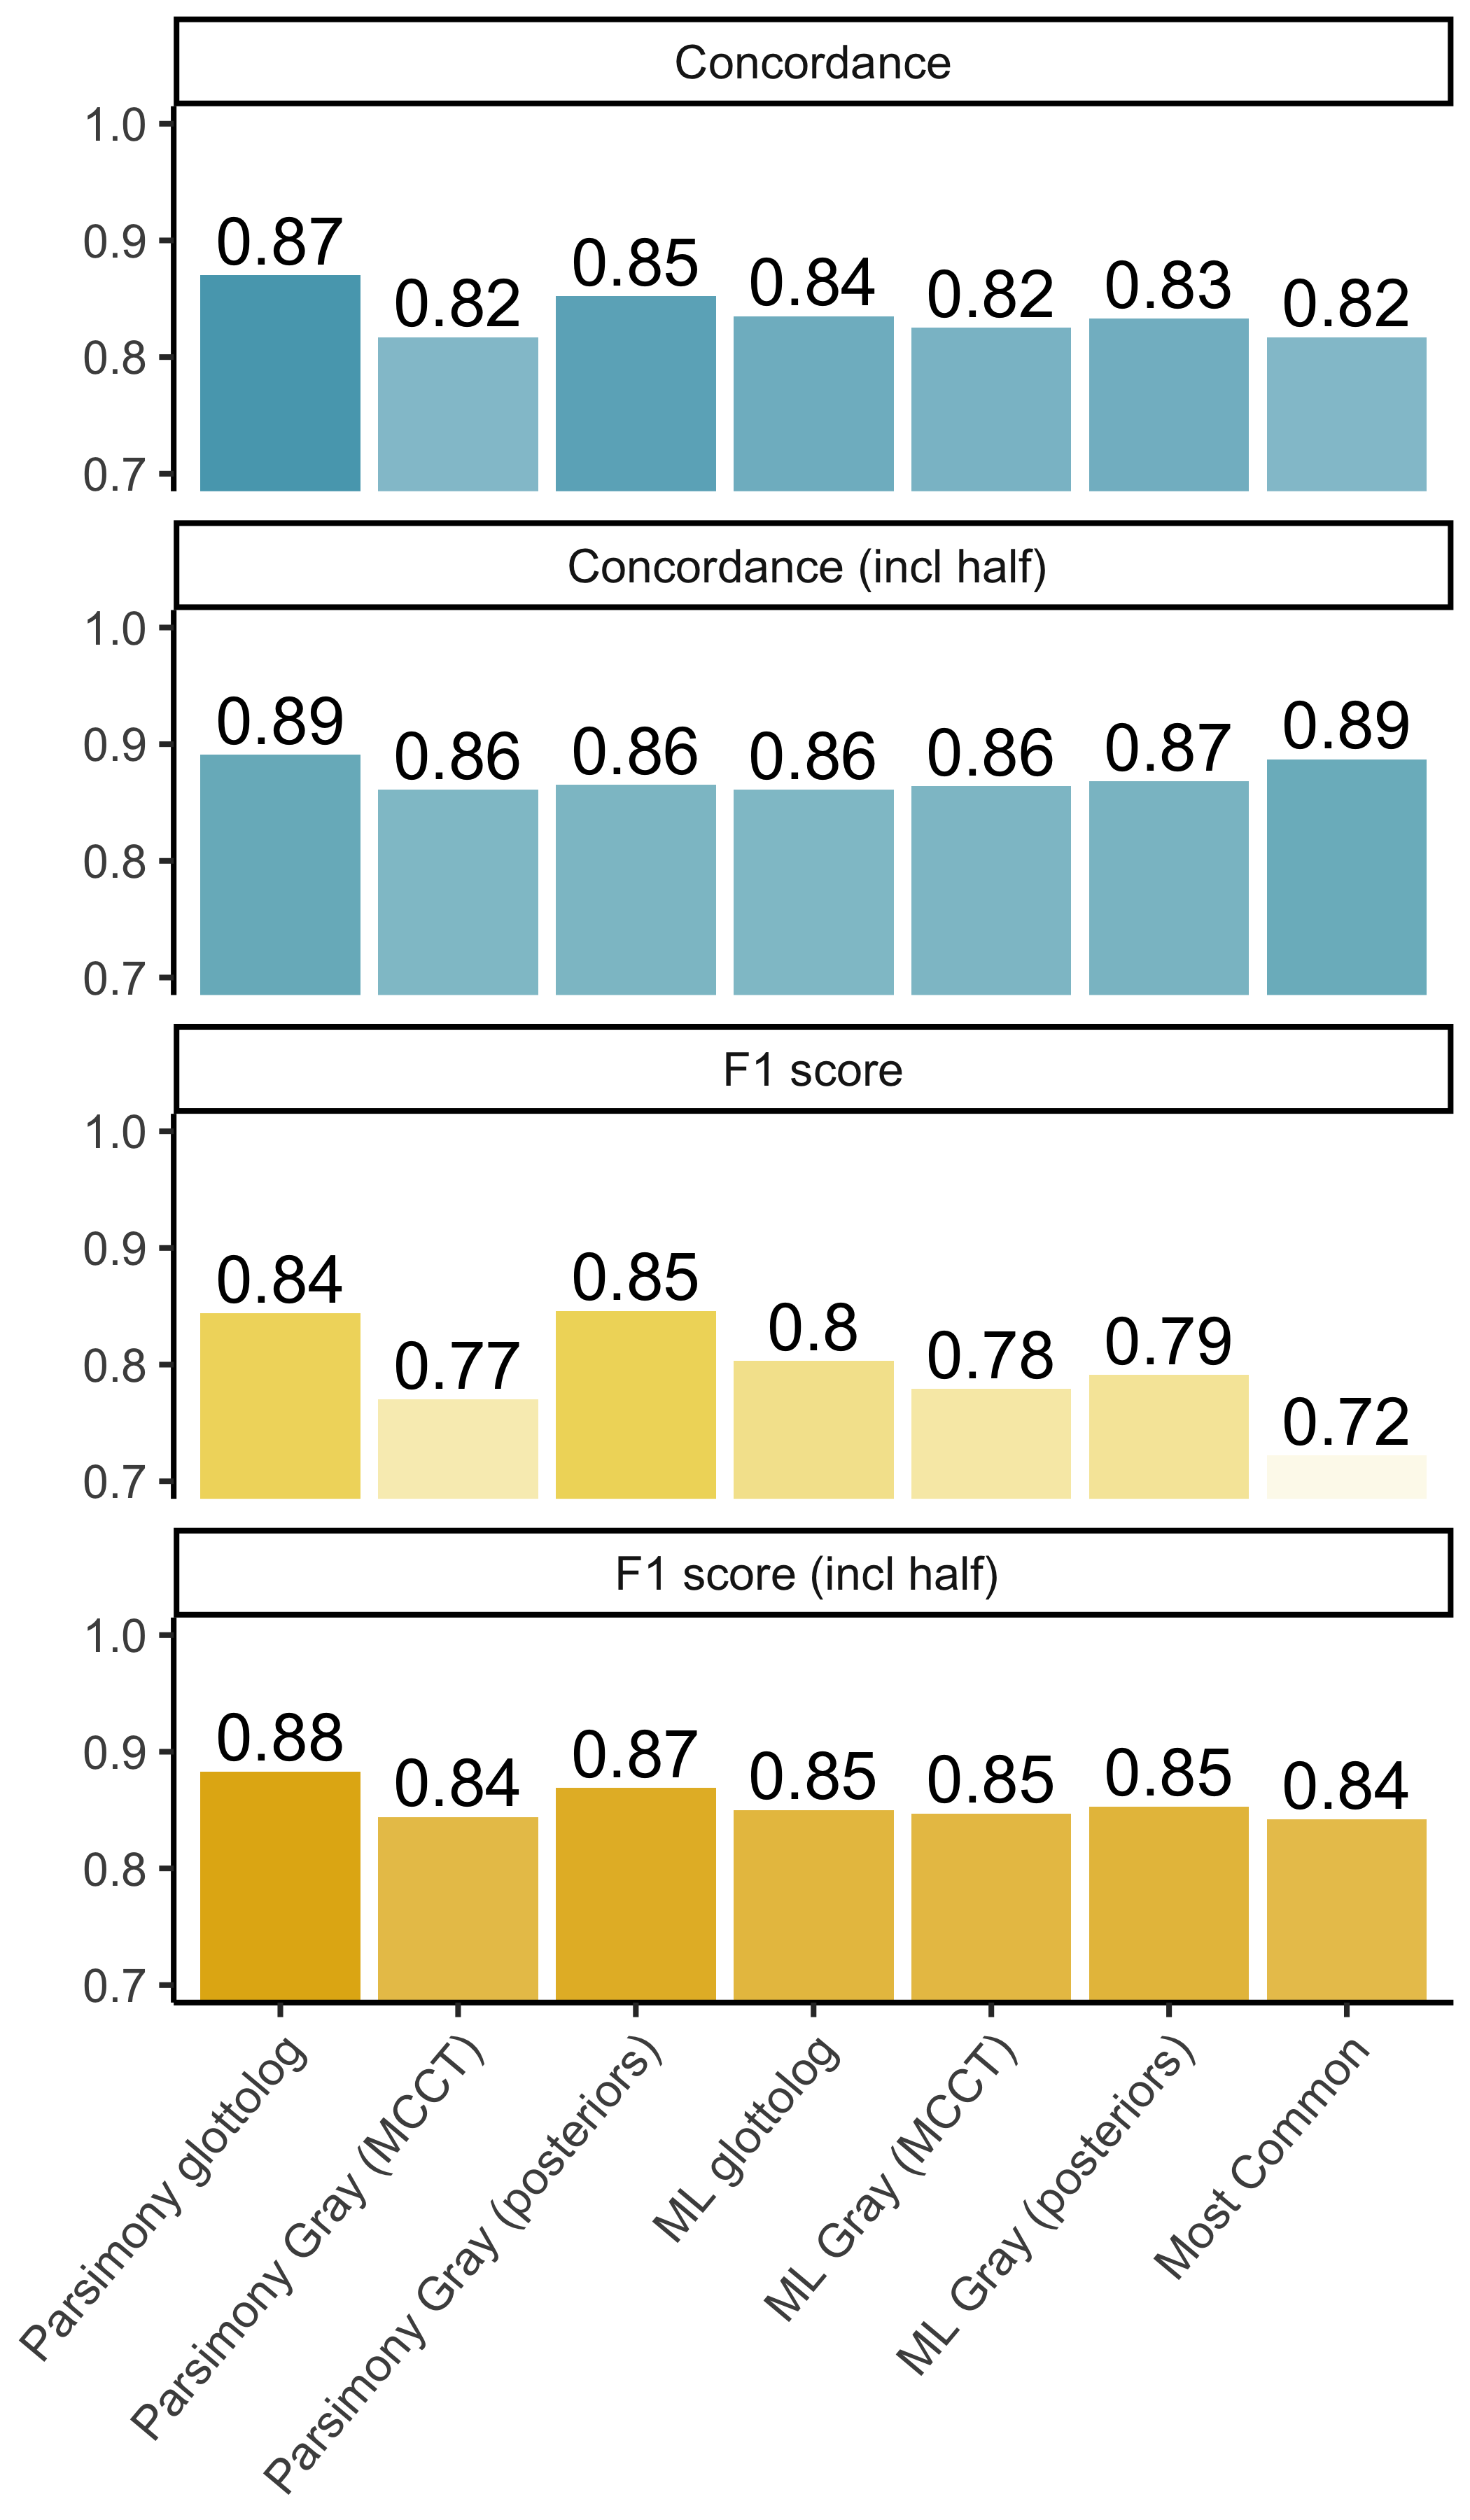
\includegraphics[width=11cm]{illustrations/plots_from_R/results/barplot_facet_scores.png}
\caption{\textbf{Barplots of concordance and F1-scores of each method.} NB that the y-axis starts from 0.7.}
\label{barplot_facet_results_incl_f1}
\end{figure}

Compared to the F1-scores from the lexical reconstruction of \citet{jager2018using}, all of the methods achieved higher scores. The highest (``best'') F1-score in \citet{jager2018using} was 0.79 (Austronesian language sample, Maximum Likelihood), and the worst was 0.44 (Indo-European, Minimal Lateral Networks). In this study, only statements about ancestral languages that could be mapped to Grambank-features were included. It is  possible that the study by \citet{jager2018using} had a greater overlap between all the reconstructions made by historical linguists and the meanings that they had data for. In that case, it is possible that the features that were possible to map to Grambank data were also those that Oceanic historical linguists are the most confident about --- hence the higher scores of agreement (quantified as F1-scores) compared to \citet{jager2018using}.

\FloatBarrier


\subsection{Mathematics of the F1-score including half-results}
\label{math_supp}

I am very grateful for the assistance of Stephen Mann in working out the mathematics of these scores as they incorporate the Half-results.

\subsubsection{Standard definitions}\label{sec:standard}

The F1-score is the harmonic mean of precision and recall \citep{van1979information}.

\begin{align*}
    F_1 &= 2\times\frac{\text{precision}\times\text{recall}}
            {\text{precision} + \text{recall}}\\
        &= \frac{\text{TP}}
            {\text{TP}+\frac{1}{2}\times(\text{FP}+\text{FN})}
\end{align*}

\begin{align*}
    \text{precision} 
        &= \frac{\text{TP}}
            {\text{TP}+\text{FP}}
\end{align*}

\begin{align*}
    \text{recall} 
        &= \frac{\text{TP}}
            {\text{TP}+\text{FN}}
\end{align*}

%%%%%%%%%%%
%%%%%%%%%%%
%%%%%%%%%%%
%%%%%%%%%%%
\subsubsection{Half-result definitions of precision and recall}\label{sec:halfsies}

The half-result-definitions of precision and recall add one half of the half-counts to the numerator, and all of the half-counts to the denominator:

\begin{equation*}
    \text{precision}_{\text{half}} 
        = \frac{\text{TP}+\frac{\text{H}}{2}}
            {\text{TP}+\text{FP}+\text{H}}
\end{equation*}

\begin{equation*}
    \text{recall}_{\text{half}}
        = \frac{\text{TP}+\frac{\text{H}}{2}}
            {\text{TP}+\text{FN}+\text{H}}
\end{equation*}

%%%%%%%%%%%
%%%%%%%%%%%
%%%%%%%%%%%
%%%%%%%%%%%
\subsubsection{The question}\label{sec:question}

We want to define $F_{1,\text{half}}$.
A natural way to do it would be to follow the rule defined above, i.e.

\begin{equation*}
    F_{1,\text{half?}} = \frac{\text{TP}+\frac{\text{H}}{2}}
            {\text{TP}+\frac{1}{2}\times(\text{FP}+\text{FN}) + \text{H}}
\end{equation*}

\noindent However, we want to ensure $F_{1,\text{half}}$ has the same relationship with $\text{precision}_{\text{half}}$ and $\text{recall}_{\text{half}}$ as $F_1$ has with precision and recall.
So we need to determine whether the following equation is true:

\begin{equation}\label{eq:question}
    2\times\frac{\text{precision}_{\text{half}}\times\text{recall}_{\text{half}}}
            {\text{precision}_{\text{half}} + \text{recall}_{\text{half}}}
    \stackrel{?}{=}
    \frac{\text{TP}+\frac{\text{H}}{2}}
            {\text{TP}+\frac{1}{2}\times(\text{FP}+\text{FN}) + \text{H}}
\end{equation}

%%%%%%%%%%%
%%%%%%%%%%%
%%%%%%%%%%%
%%%%%%%%%%%
\subsubsection{The proof}\label{sec:proof}

We will expand the left-hand side of \eqref{eq:question} and show it is equal to the right-hand side.
Let's forget about the $2\times$ for now (we will reintroduce it at the end).
Expanding the numerator gives:

\begin{equation*}
    \frac{\left(
        \text{TP}+\frac{\text{H}}{2}
    \right)\left(
        \text{TP}+\frac{\text{H}}{2}
    \right)}
    {\left(
        \text{TP} + \text{FP} + \text{H}
    \right)\left(
        \text{TP} + \text{FN} + \text{H}
    \right)}
\end{equation*}

\noindent Expanding the denominator gives:

\begin{align*}
    &\frac{\text{TP}+\frac{\text{H}}{2}}
    {\text{TP}+\text{FP}+\text{H}}
    +
    \frac{\text{TP}+\frac{\text{H}}{2}}
    {\text{TP}+\text{FN}+\text{H}}\\[1.5ex]
    &=
    %% Second line, left part
    %% Numerator
    \frac{\left(
        \text{TP}+\frac{\text{H}}{2}
    \right)\left(
        \text{TP}+\text{FN}+\text{H}
    \right)}
    %% Denominator
    {\left(
        \text{TP}+\text{FP}+\text{H}
    \right)\left(
        \text{TP}+\text{FN}+\text{H}
    \right)}
    +
    %% Second line, right part
    %% Numerator
    \frac{\left(
        \text{TP}+\frac{\text{H}}{2}
    \right)\left(
        \text{TP}+\text{FP}+\text{H}
    \right)}
    %% Denominator
    {\left(
        \text{TP}+\text{FN}+\text{H}
    \right)\left(
        \text{TP}+\text{FP}+\text{H}
    \right)}\\[1.5ex]
    %% Third line
    &=\frac{\left(
        \text{TP}+\frac{\text{H}}{2}
    \right)\left(
        2\times\text{TP} + \text{FP} + \text{FN} + 2\times\text{H}
    \right)}
    {\left(
        \text{TP}+\text{FP}+\text{H}
    \right)\left(
        \text{TP}+\text{FN}+\text{H}
    \right)}
\end{align*}

\noindent When we put the numerator back on top of the denominator, both of their respective denominators cancel out, because they are both $(\text{TP}+\text{FP}+\text{H})(\text{TP}+\text{FN}+\text{H})$.
So we end up with \emph{the numerator of the numerator} on top of \emph{the numerator of the denominator}, like so:

\begin{align*}
    &\frac{\left(
        \text{TP}+\frac{\text{H}}{2}
    \right)\left(
        \text{TP}+\frac{\text{H}}{2}
    \right)}
    {\left(
        \text{TP}+\frac{\text{H}}{2}
    \right)\left(
        2\times\text{TP} + \text{FP} + \text{FN} + 2\times\text{H}
    \right)}\\[1.5ex]
    &=
    \frac{\left(
        \text{TP}+\frac{\text{H}}{2}
    \right)}
    {2\times\text{TP} + \text{FP} + \text{FN} + 2\times\text{H}}
\end{align*}

\noindent Finally, we bring back the $2\times$ from the beginning:

\begin{align*}
    &2\times\frac{\left(
        \text{TP}+\frac{\text{H}}{2}
    \right)}
    {2\times\text{TP} + \text{FP} + \text{FN} + 2\times\text{H}}\\[1ex]
    &=
    \frac{\text{TP}+\frac{\text{H}}{2}}
    {\text{TP} + \frac{1}{2}\times(\text{FP} + \text{FN}) + \text{H}}
\end{align*}

\noindent And we have our suggested definition of $F_{1,\text{half}}$ as required.

\FloatBarrier


%


\subsection{Further details on the tree phylogeny}
\label{supp:tree_details}

The tree from \citet{grayetal_2009} contains duplicates in terms of glottocodes (see for example Nakanai). This is because it is a tree of word-lists for languages (doculects) rather than languages themselves. There are also some instances where multiple dialects of one language are included. For the analysis, only one tip per language was retained, based on which had best coverage in the underlying data for the tree (i.e. the Austronesian Basic Vocabulary Database, ABVD \citep{ABVD}). This means that duplicate glottocodes were reduced to one, be it due to multiple word-lists or dialects. The specific analytical choices are found in the following three R-scripts:

\begin{itemize}
\item Oceanic\_computational\_ASR/code/01\_requirements.R
\item Oceanic\_computational\_ASR/code/analysis\_scripts\_gray\_mcct/\\03\_get\_gray\_tree\_mcct.R
\item Oceanic\_computational\_ASR/code/analysis\_scripts\_gray\_all\_posterior/\\03\_process\_gray\_tree\_posteriors.R
\end{itemize}

For both Maximum Parsimony and Maximum Likelihood the tree were first pruned down to only languages where there is data in Grambank for each given feature, i.e. the ASR-analysis never contains tips with missing or ambiguous data. Missing data varies with features, so each analysis per tree and method differs in number of tips.

%For the further Maximum Parsimony analysis, tips representing languages where the data for a particular feature was missing were dropped for the analysis of that feature. For the Maximum Likelihood analysis, the value at such tips was converted to ambiguous. This is necessary because otherwise the rate of change across the different features would not be comparable in the Maximum Likelihood analysis.

Regarding branch lengths, most of the trees in the analysis are not ultrametric, i.e. the distances between the tips and the roots are not all the same. If we use trees to represent history and time, then an ultrametric, or near-Ultrametric, tree is a more reasonable representation of said histories when we assume that the languages at the tips existed at the same time. Fig \ref{fig:branch_lengths} illustrates different configurations of branch lengths using only Nuclear Polynesian languages. It is reasonable to assume that the data gathered on these languages represent similar time-slices to each other, i.e. the representation of Rapa Nui is not considerably ``younger'' as a language than Tongan. If the tips included ancient languages, such as Sanskrit or Akkadian, it may be possible for such tips to have a shorter distance to the root than the others. However, if the languages are of a similar ``age'', the tree ought to be ultrametric or near-ultrametric if we understand tree length as representing time.

The Glottolog genealogical classification follows common principles in historical linguistics by focusing on the validity of sub-grouping, not branch lengths. The Glottolog 4.5 tree does not include any information about branch lengths. This is interpreted as the same as if all branches are of the same length (they are explicitly all set to 1 in the analysis). In order to illustrate what this entails, consider the difference between Fig. \ref{glottolog_example_poly_1} and Fig. \ref{glottolog_example_poly_grafen}. The first is the Glottolog tree of Nuclear Polynesian as found originally, i.e. with all branches of the same length (1). The second is a transformation of the first, it has been made ultrametric by Grafen's transform \citep{grafen1989phylogenetic}, which is one of several approaches to making a tree ultrametric in lieu of branch lengths directly from the data. The second tree is \emph{not} used in the analysis, it is included here only to illustrate how the same sub-grouping of languages can be expressed when the branch lengths are changed. Transformations of branch lengths should be carried out with great care and with good reason. It is not clear what transformation of branch lengths in the Glottolog 4.5-tree is appropriate, which is why none has been carried out in the analysis of this paper. Keeping the Glottolog 4.5-tree lacking branch lengths may also be more true to historical linguistics methodology.

The branch lengths in the trees from \citet{grayetal_2009} are derived from the dynamics of the data --- the word-lists --- and certain priors regarding island settlement. The MCC-tree of \citet{grayetal_2009} is not ultrametric, but very close to it (see Fig \ref{gray_tree_branch_example}. After pruning to the subset that overlaps with Oceanic languages in Grambank (as described above), the difference between the tip with the largest distance to the root and the smallest is tiny (3.408377 -  3.408362). In the random sample of 100 from the 4,200 posteriors trees, the case is the same as with the MCCT --- they are not perfectly ultrametric but very close (see Fig \ref{gray_tree_branch_example_posteriors}. The trees from \citet{grayetal_2009} may not be perfectly ultrametric, but they are much more closer to ultrametric than the Glottolog tree, as can be seen by comparing the visualisations in Fig \ref{fig:branch_lengths}.

\begin{figure}[ht]
\centering
    \begin{subfigure}{0.5\linewidth}
      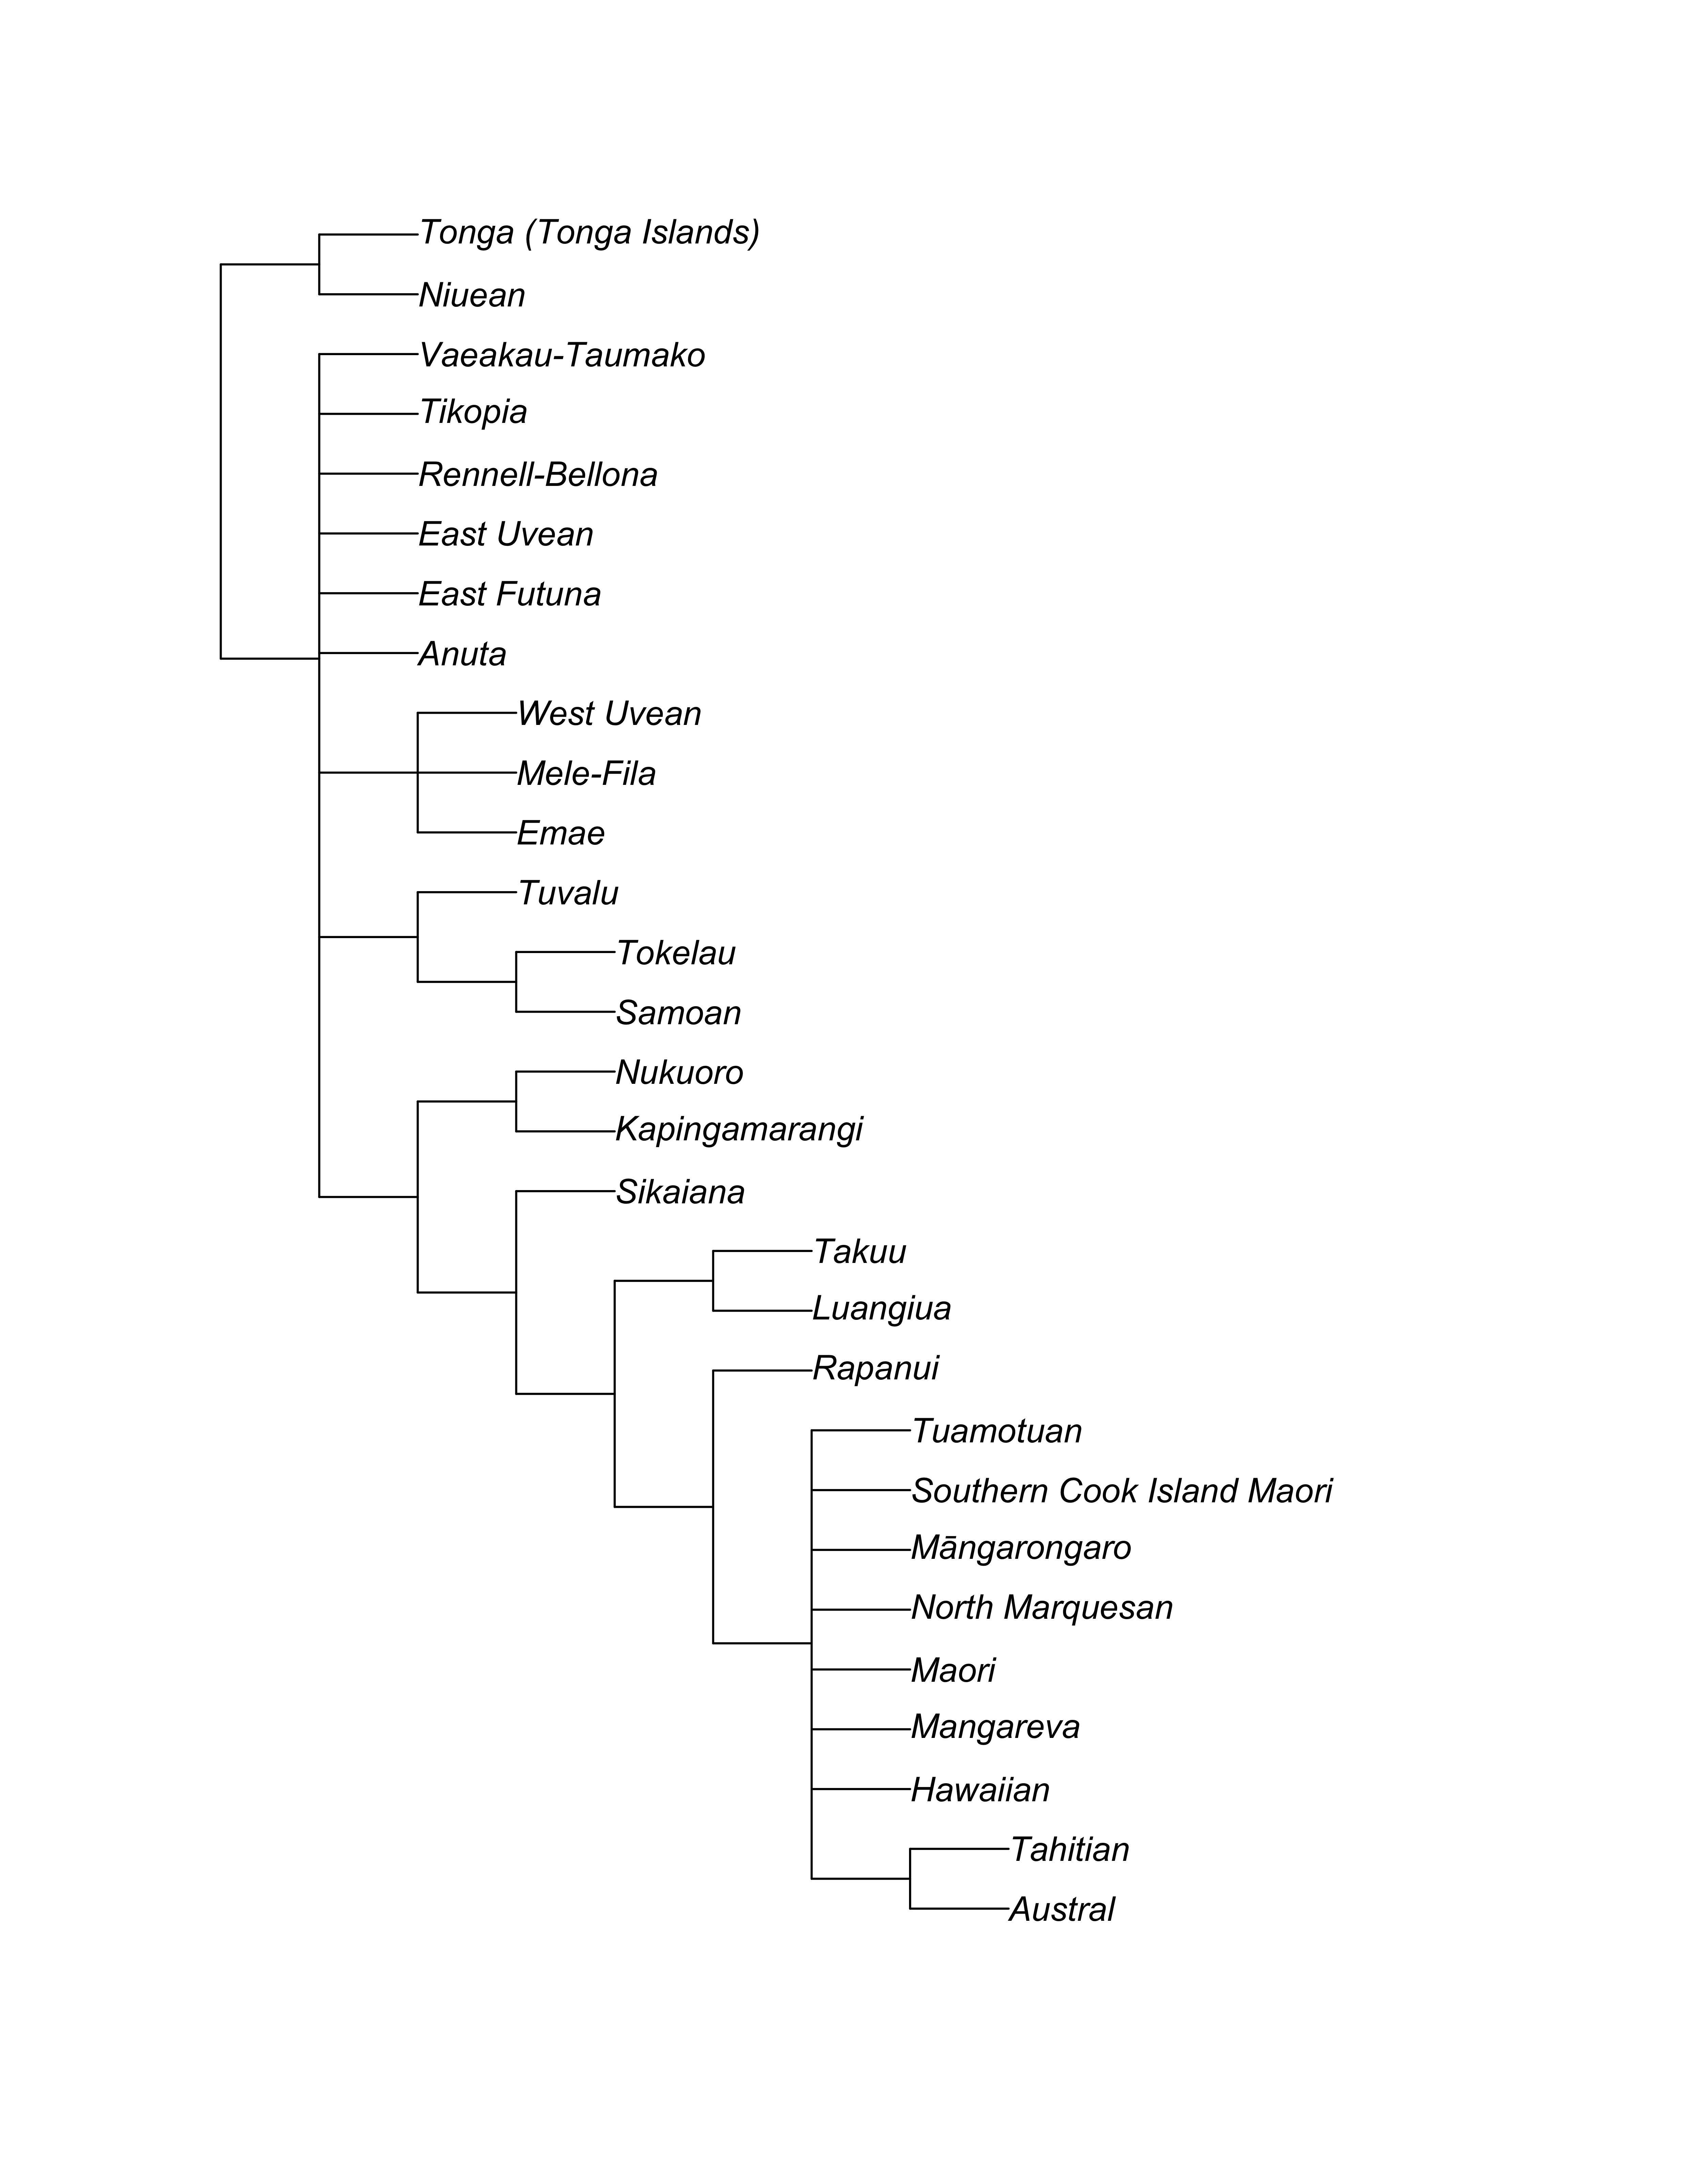
\includegraphics[width=\textwidth]{illustrations/plots_from_R/tree_plots/poly_tree_example_brlen_glottolog_1}
    \caption{Glottolog tree, all branches have the same length.}
    \label{glottolog_example_poly_1}
    \end{subfigure}
\hfil
    \begin{subfigure}{0.5\linewidth}
          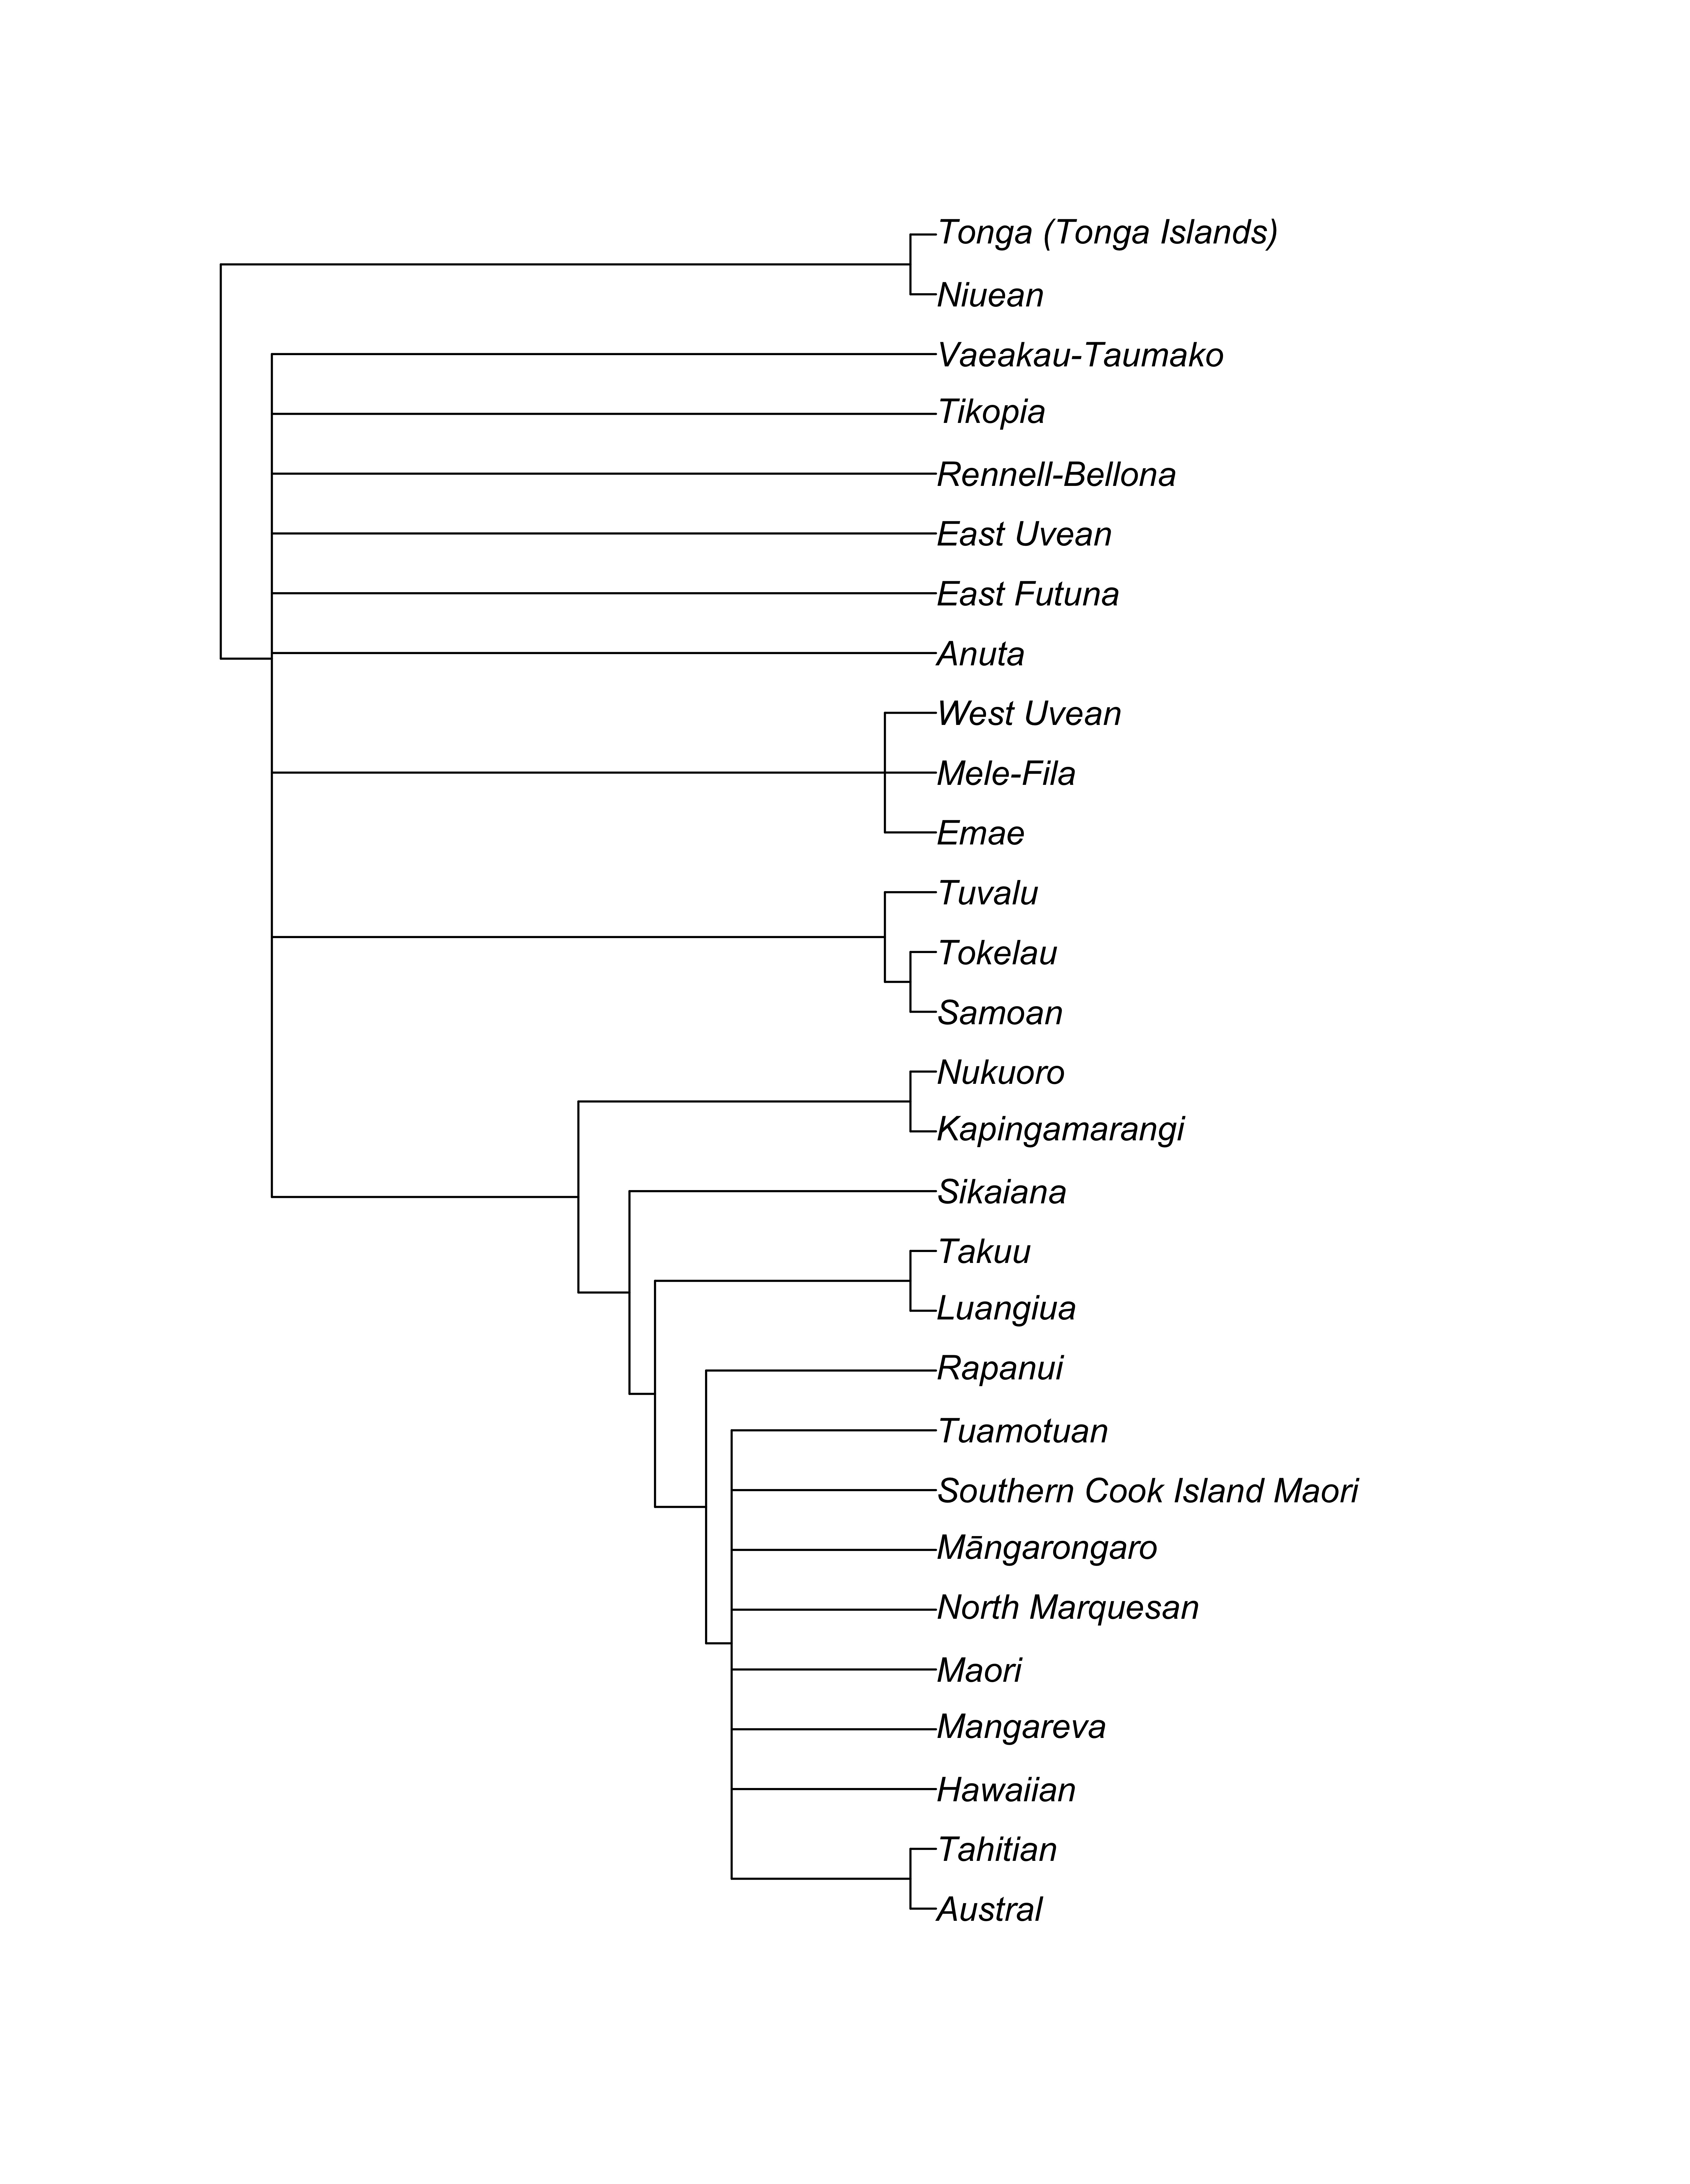
\includegraphics[width=\textwidth]{illustrations/plots_from_R/tree_plots/poly_tree_example_brlen_glottolog_grafen.png}
     \caption{Glottolog tree, made ultrametric with Grafen's method \citep{grafen1989phylogenetic}.}
      \label{glottolog_example_poly_grafen}
    \end{subfigure}

    \begin{subfigure}{0.5\linewidth}
          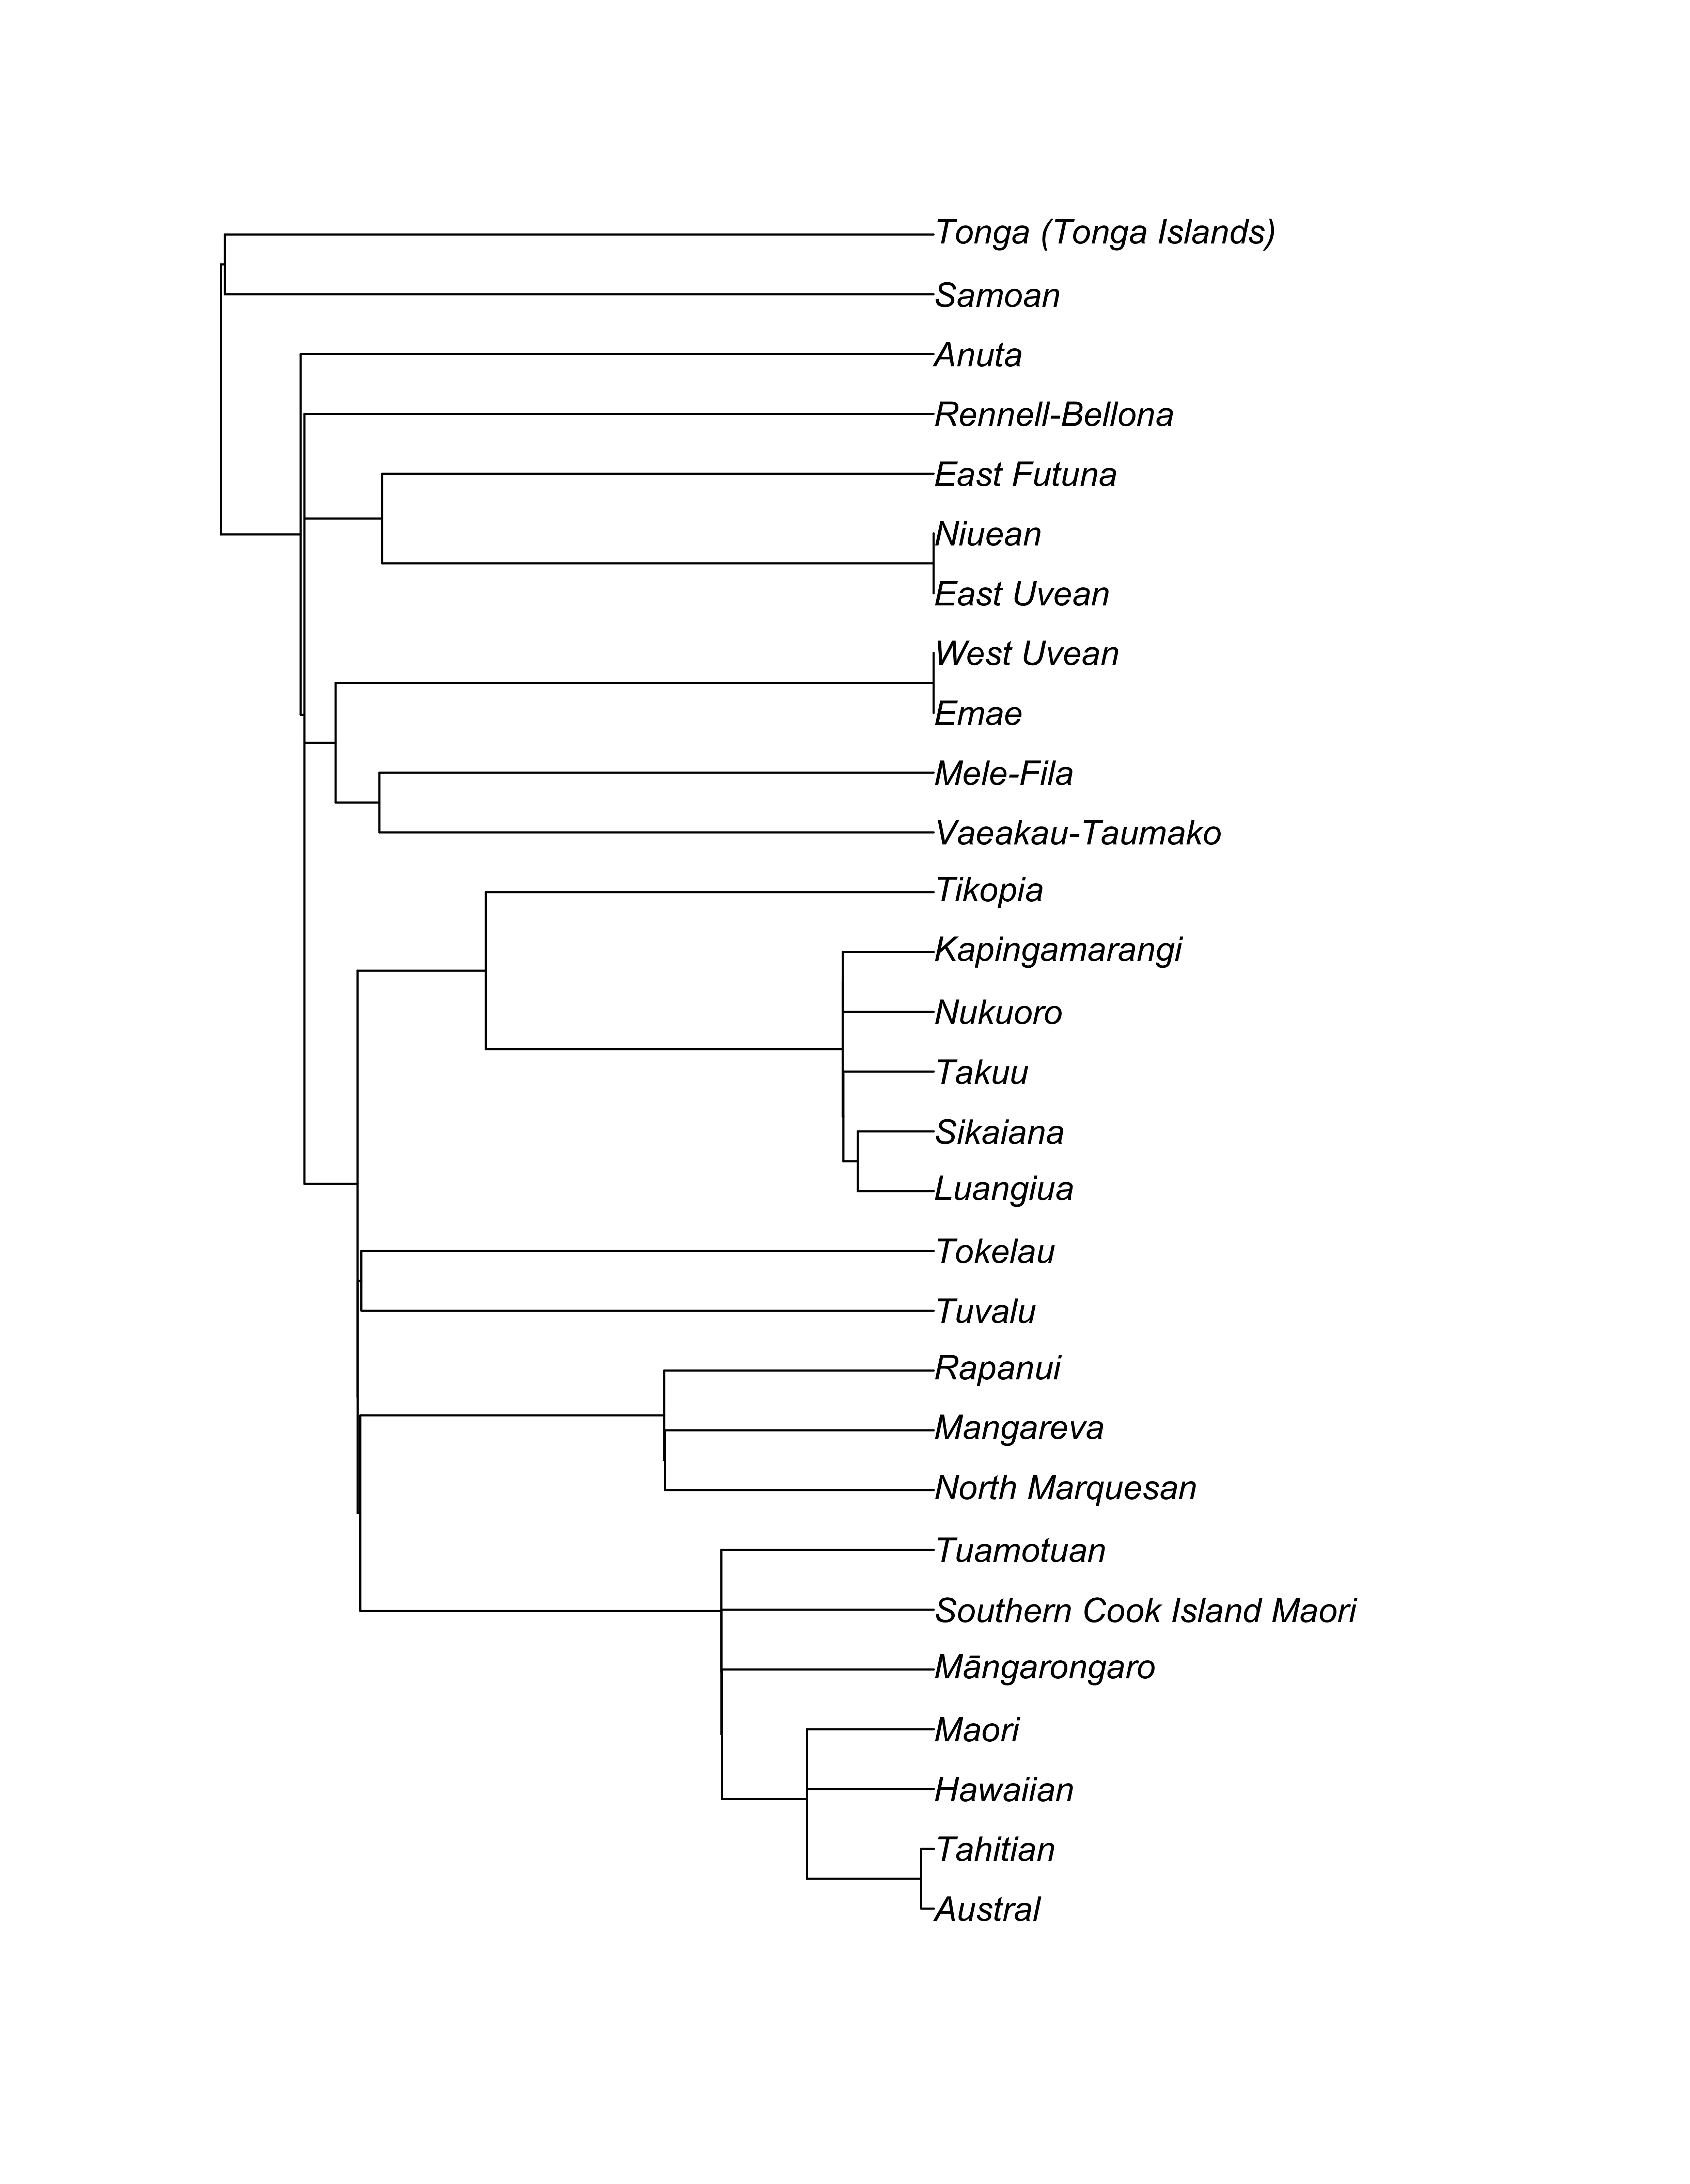
\includegraphics[width=\textwidth]{illustrations/plots_from_R/tree_plots/poly_tree_example_brlen_gray.png}
    \caption{\citet{grayetal_2009} MCCT.}
     \label{gray_tree_branch_example}
    \end{subfigure}
\hfil
    \begin{subfigure}{0.5\linewidth}
          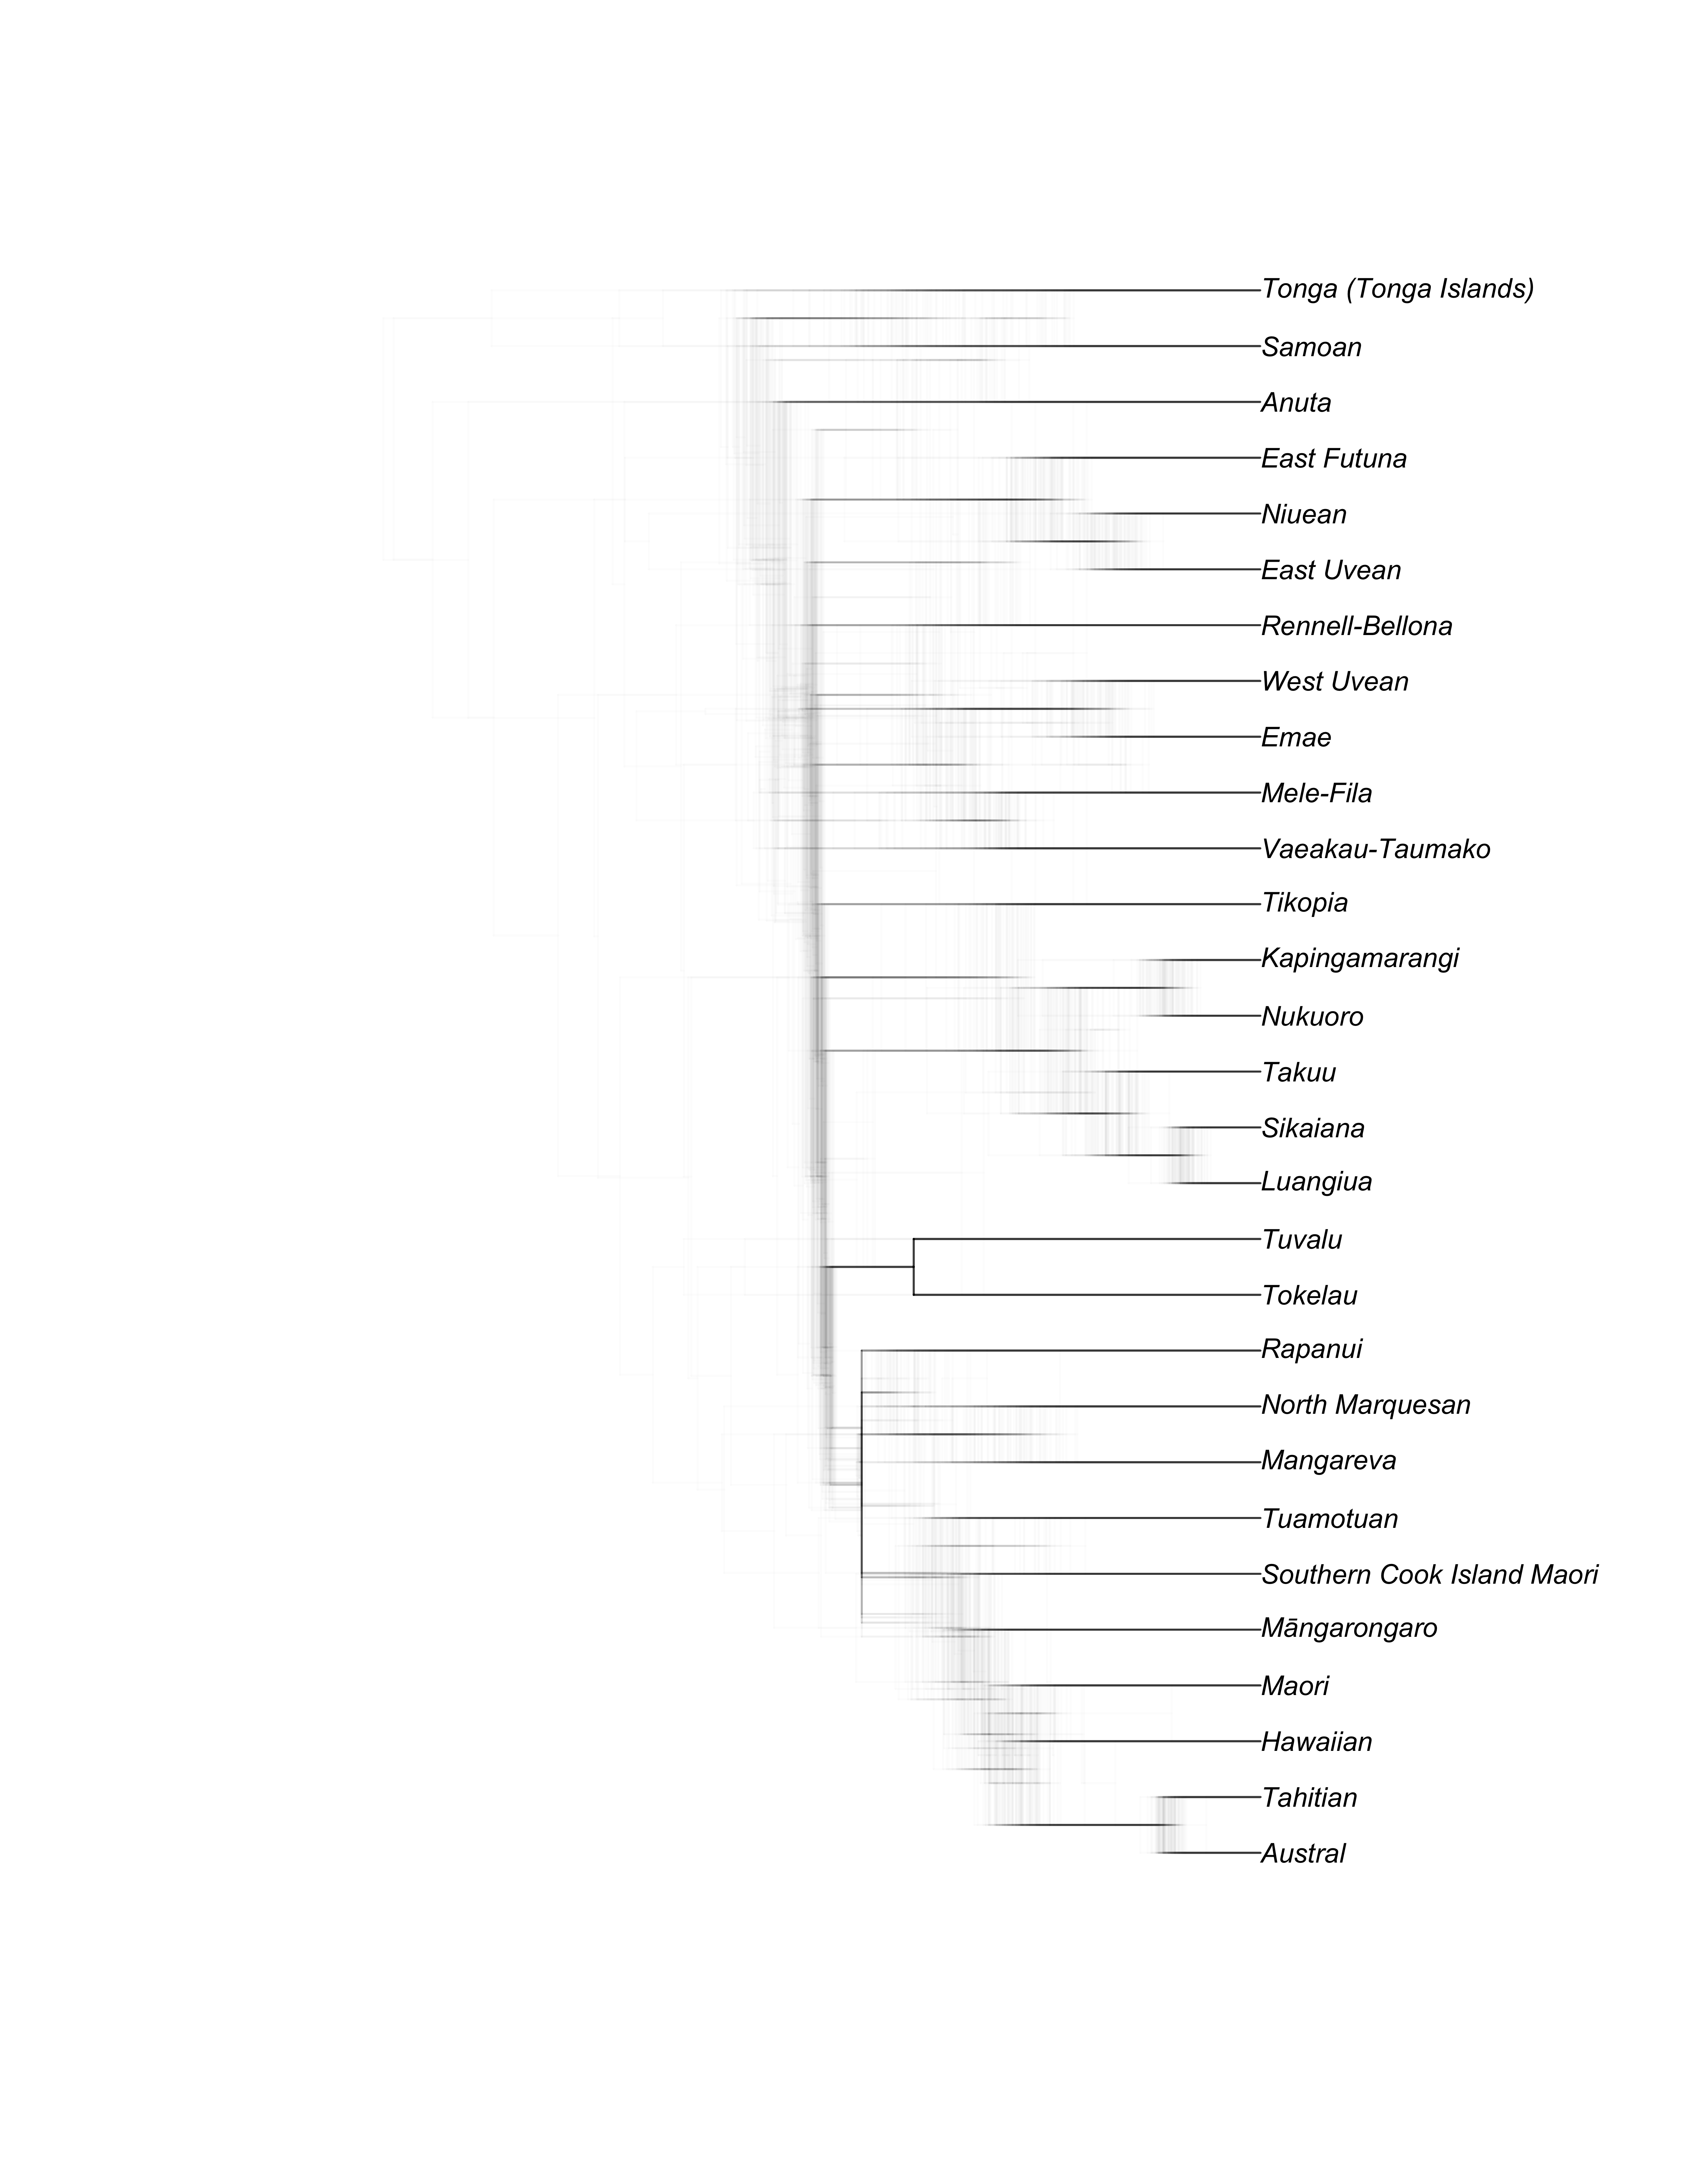
\includegraphics[width=\textwidth]{illustrations/plots_from_R/tree_plots/poly_tree_example_brlen_gray_posterios.png}
    \caption{\citet{grayetal_2009} posteriors tree (random sample of 100). The densitree-visualisation is in phylogram-style.}
     \label{gray_tree_branch_example_posteriors}
    \end{subfigure}
    
\caption{Four trees of Nuclear Polynesian, demonstrating branch lengths.}
    \label{fig:branch_lengths}
\end{figure}

Concerning binary splits, there are non-binary splits in the Glottolog 4.5 tree, the \citet{grayetal_2009} MCCT and in 64 of the 100 posterior trees. For this analysis, we have chosen to not resolve these polytomies into binary splits in order to stay as true as possible to the original phylogeny. There are branches of length 0 in the MCCT and posterior trees. It is not possible to collapse these into polytomies as this may in cases introduce basal polytomies. Instead, 0.00011 length was added to all branches. Doing this removes branches of length 0 while maintaining the relative lengths of all branches in the tree.

In some cases, pruning a given posterior tree to the relevant tips resulted in the tree becoming unrooted. In such cases, the tree was re-rooted using midpoint rooting \texttt{castor::root\_at\_midpoint()} \cite{R-castor}. There were 4 such cases in the random sample of posteriors trees (random seed = 147).

All of the wrangling of the trees is found in the data analysis R-scripts that accompany this paper.
\FloatBarrier    


\subsection{Further details on the Grambank coding of proto-languages }
\label{supp:proto_lg_coding}
Another example of how information in the publications was turned into Grambank feature coding relates to verbal markers encoding subjects and objects, as proposed by \citet{lynchrosscrowley_proto_grammar_oceanic} among others. In their book, there is a paper on reconstructions of grammar for Proto-Oceanic and in the section on the basic verb phrase we find the statement below:

\begin{quotation}
\noindent\emph{Attached to the verb root were a subject proclitic and, if the verb had a non-generic object, an object enclitic.} \end{quotation} \begin{flushright} \citet[83]{lynchrosscrowley_proto_grammar_oceanic} \end{flushright}

This statement, together with a verb schema provided in the section, support the notion that Proto-Oceanic had subject proclitics and object enclitics. We can also infer from this publication as a whole that the authors believe Proto-Oceanic in fact did \emph{not} have subject \emph{en}clitics and object \emph{pro}clitics. This second prediction relies on absence of evidence and is less strong than the first, but given that the whole paper is void of any description of object proclitics or subject enclitics being a possibility (including the verb schema) and argument structure is well-discussed, we may dare to make this leap. This information can be translated into the Grambank questionnaire by positing absence and presence for the six relevant features that concern argument marking on the verb (where S stands for subject of intransitive, A for subject of transitive and O for object; see table~\ref{example_HL_prediction_table}).

 %one of ste's favourite tables
\begin{table}
\caption{Example of predictions from historical linguistics as rendered in Grambank features.}
\label{example_HL_prediction_table}

\begin{tabular}{|p{3cm}| p{4.5cm}|  p{2.5cm}| p{2.5cm} | p{3cm} |p{2cm}| }
\hline
\textbf{Grambank ID} & \textbf{Question} & \textbf{Proto-language} & \textbf{Expert prediction} & \textbf{Reference} \\ 
\hline
GB089  &Can the S argument be indexed by a suffix/enclitic on the verb in the simple main clause? &Proto-Oceanic &Absent & \citet[498-499]{ross2004morphosyntactic}, \citet[83]{lynchrosscrowley_proto_grammar_oceanic} \\ \hline
GB090 &Can the S argument be indexed by a prefix/proclitic on the verb in the simple main clause? &Proto-Oceanic &Present &\citet[498-499]{ross2004morphosyntactic}, \citet[83]{lynchrosscrowley_proto_grammar_oceanic}  \\ \hline
GB091 &Can the A argument be indexed by a suffix/enclitic on the verb in the simple main clause? &Proto-Oceanic &Absent &\citet[498-499]{ross2004morphosyntactic}, \citet[83]{lynchrosscrowley_proto_grammar_oceanic} \\ \hline
GB092  &Can the A argument be indexed by a prefix/proclitic on the verb in the simple main clause? &Proto-Oceanic &Present &\citet[498-499]{ross2004morphosyntactic}, \citet[83]{lynchrosscrowley_proto_grammar_oceanic}  \\ \hline
GB093  &Can the P argument be indexed by a suffix/enclitic on the verb in the simple main clause? &Proto-Oceanic &Present &\citet[498-499]{ross2004morphosyntactic}, \citet[83]{lynchrosscrowley_proto_grammar_oceanic} \\ \hline
GB094  &Can the P argument be indexed by a prefix/proclitic on the verb in the simple main clause? &Proto-Oceanic &Absent & \citet[498-499]{ross2004morphosyntactic}, \citet[83]{lynchrosscrowley_proto_grammar_oceanic} \\ \hline
\end{tabular}
\end{table}



\FloatBarrier
%\subsection{Table of new predictions}
%\label{asr_table_extra}
%\begin{landscape}
%% latex table generated in R 4.2.3 by xtable 1.8-4 package
% Mon Jun 12 21:27:07 2023
\begin{longtable}{p{1.5cm}p{2.5cm}p{2.5cm}p{2.5cm}p{2.5cm}p{2.5cm}p{2.5cm}p{2.5cm}}
  \toprule
Feature\_ID & Glottolog Parsimony & Gray parismony -MCCT & Gray parismony -posteriors & Glottolog ML & Gray ML -MCCT & Gray ML -posteriors & Most Common \\ 
  \midrule
GB024a & Present & Present & Present & Present & Present & Present & Present \\ 
  GB024b & Present & Present & Present & Present & Present & Present & Present \\ 
  GB024b & Present & Present & Present & Present & Present & Present & Present \\ 
  GB024b & Present & Present & Present & Present & Present & Present & Present \\ 
  GB024b & Present & Present & Present & Present & Present & Present & Absent \\ 
  GB025a & Present & Present & Present & Present & Present & Present & Present \\ 
  GB025b & Present & Present & Present & Present & Present & Present & Present \\ 
  GB025b & Present & Present & Present & Present & Present & Present & Present \\ 
  GB065b & Present & Present & Present & Present & Present & Present & Present \\ 
  GB065b & Present & Present & Present & Present & Present & Present & Present \\ 
  GB065b & Present & Present & Present & Present & Present & Present & Present \\ 
  GB130a & Present & Present & Present & Present & Present & Present & Present \\ 
  GB130b & Present & Present & Present & Present & Present & Present & Present \\ 
  GB193b & Present & Present & Present & Present & Present & Present & Present \\ 
  GB193b & Present & Present & Present & Present & Present & Present & Present \\ 
  GB203b & Present & Present & Present & Present & Present & Present & Present \\ 
  GB203b & Present & Present & Present & Present & Present & Present & Present \\ 
  GB203b & Present & Present & Present & Present & Present & Present & Present \\ 
  GB203b & Present & Present & Present & Present & Present & Present & Present \\ 
  GB020 & Present & Present & Present & Present & Present & Present & Present \\ 
  GB021 & Present & Present & Present & Present & Present & Present & Present \\ 
  GB022 & Present & Present & Present & Present & Present & Present & Present \\ 
  GB027 & Present & Present & Present & Present & Present & Present & Present \\ 
  GB028 & Present & Present & Present & Present & Present & Present & Present \\ 
  GB028 & Present & Present & Present & Present & Present & Present & Present \\ 
  GB031 & Present & Present & Present & Present & Present & Present & Present \\ 
  GB031 & Present & Present & Present & Present & Present & Present & Present \\ 
  GB035 & Present & Present & Present & Present & Present & Present & Present \\ 
  GB035 & Present & Present & Present & Present & Present & Present & Present \\ 
  GB047 & Present & Present & Present & Present & Present & Present & Present \\ 
  GB047 & Present & Present & Present & Present & Present & Present & Present \\ 
  GB047 & Present & Present & Present & Present & Present & Present & Present \\ 
  GB057 & Present & Present & Present & Present & Present & Present & Present \\ 
  GB059 & Present & Present & Present & Present & Present & Present & Present \\ 
  GB059 & Present & Present & Present & Present & Present & Present & Present \\ 
  GB068 & Present & Present & Present & Present & Present & Present & Present \\ 
  GB068 & Present & Present & Present & Present & Present & Present & Present \\ 
  GB068 & Present & Present & Present & Present & Present & Present & Present \\ 
  GB074 & Present & Present & Present & Present & Present & Present & Present \\ 
  GB074 & Present & Present & Present & Present & Present & Present & Present \\ 
  GB079 & Present & Present & Present & Present & Present & Present & Present \\ 
  GB079 & Present & Present & Present & Present & Present & Present & Present \\ 
  GB080 & Present & Present & Present & Present & Present & Present & Present \\ 
  GB080 & Present & Present & Present & Present & Present & Present & Present \\ 
  GB093 & Present & Present & Present & Present & Present & Present & Absent \\ 
  GB113 & Present & Present & Present & Present & Present & Present & Present \\ 
  GB124 & Present & Present & Present & Present & Present & Present & Present \\ 
  GB124 & Present & Present & Present & Present & Present & Present & Present \\ 
  GB126 & Present & Present & Present & Present & Present & Present & Present \\ 
  GB126 & Present & Present & Present & Present & Present & Present & Present \\ 
  GB126 & Present & Present & Present & Present & Present & Present & Present \\ 
  GB126 & Present & Present & Present & Present & Present & Present & Present \\ 
  GB131 & Present & Present & Present & Present & Present & Present & Present \\ 
  GB134 & Present & Present & Present & Present & Present & Present & Present \\ 
  GB134 & Present & Present & Present & Present & Present & Present & Present \\ 
  GB134 & Present & Present & Present & Present & Present & Present & Present \\ 
  GB134 & Present & Present & Present & Present & Present & Present & Present \\ 
  GB135 & Present & Present & Present & Present & Present & Present & Present \\ 
  GB135 & Present & Present & Present & Present & Present & Present & Present \\ 
  GB135 & Present & Present & Present & Present & Present & Present & Present \\ 
  GB135 & Present & Present & Present & Present & Present & Present & Present \\ 
  GB139 & Present & Present & Present & Present & Present & Present & Present \\ 
  GB139 & Present & Present & Present & Present & Present & Present & Present \\ 
  GB139 & Present & Present & Present & Present & Present & Present & Present \\ 
  GB155 & Present & Present & Present & Present & Present & Present & Present \\ 
  GB155 & Present & Present & Present & Present & Present & Present & Present \\ 
  GB158 & Present & Present & Present & Present & Present & Present & Present \\ 
  GB158 & Present & Present & Present & Present & Present & Present & Present \\ 
  GB158 & Present & Present & Present & Present & Present & Present & Present \\ 
  GB159 & Present & Present & Present & Present & Present & Present & Present \\ 
  GB159 & Present & Present & Present & Present & Present & Present & Present \\ 
  GB159 & Present & Present & Present & Present & Present & Present & Present \\ 
  GB254 & Present & Present & Present & Present & Present & Present & Present \\ 
  GB254 & Present & Present & Present & Present & Present & Present & Present \\ 
  GB254 & Present & Present & Present & Present & Present & Present & Present \\ 
  GB254 & Present & Present & Present & Present & Present & Present & Present \\ 
  GB257 & Present & Present & Present & Present & Present & Present & Present \\ 
  GB257 & Present & Present & Present & Present & Present & Present & Present \\ 
  GB257 & Present & Present & Present & Present & Present & Present & Present \\ 
  GB257 & Present & Present & Present & Present & Present & Present & Present \\ 
  GB299 & Present & Present & Present & Present & Present & Present & Present \\ 
  GB299 & Present & Present & Present & Present & Present & Present & Present \\ 
  GB301 & Present & Present & Present & Present & Present & Present & Present \\ 
  GB301 & Present & Present & Present & Present & Present & Present & Present \\ 
  GB301 & Present & Present & Present & Present & Present & Present & Present \\ 
  GB304 & Present & Present & Present & Present & Present & Present & Present \\ 
  GB318 & Present & Present & Present & Present & Present & Present & Present \\ 
  GB326 & Present & Present & Present & Present & Present & Present & Present \\ 
  GB326 & Present & Present & Present & Present & Present & Present & Present \\ 
  GB326 & Present & Present & Present & Present & Present & Present & Present \\ 
  GB326 & Present & Present & Present & Present & Present & Present & Present \\ 
  GB327 & Present & Present & Present & Present & Present & Present & Present \\ 
  GB327 & Present & Present & Present & Present & Present & Present & Present \\ 
  GB327 & Present & Present & Present & Present & Present & Present & Present \\ 
  GB333 & Present & Present & Present & Present & Present & Present & Present \\ 
  GB333 & Present & Present & Present & Present & Present & Present & Present \\ 
  GB333 & Present & Present & Present & Present & Present & Present & Present \\ 
  GB421 & Present & Present & Present & Present & Present & Present & Half \\ 
  GB433 & Present & Present & Present & Present & Present & Present & Absent \\ 
  GB519 & Present & Present & Present & Present & Present & Present & Present \\ 
  GB519 & Present & Present & Present & Present & Present & Present & Present \\ 
  GB520 & Present & Present & Present & Present & Present & Present & Present \\ 
  GB521 & Present & Present & Present & Present & Present & Present & Present \\ 
  GB521 & Present & Present & Present & Present & Present & Present & Present \\ 
  GB522 & Present & Present & Present & Present & Present & Present & Present \\ 
   \bottomrule
\caption{Table showing predictions where the six MP and ML methods agree on presence} 
\label{extra_predictions_table}
\end{longtable}

%\end{landscape}

%\subsection{Supplementary Figures}
%\label{supp:supplementary _figures}




\end{document}
